\documentclass[twoside]{book}

% Packages required by doxygen
\usepackage{fixltx2e}
\usepackage{calc}
\usepackage{doxygen}
\usepackage[export]{adjustbox} % also loads graphicx
\usepackage{graphicx}
\usepackage[utf8]{inputenc}
\usepackage{makeidx}
\usepackage{multicol}
\usepackage{multirow}
\PassOptionsToPackage{warn}{textcomp}
\usepackage{textcomp}
\usepackage[nointegrals]{wasysym}
\usepackage[table]{xcolor}

% Font selection
\usepackage[T1]{fontenc}
\usepackage[scaled=.90]{helvet}
\usepackage{courier}
\usepackage{amssymb}
\usepackage{sectsty}
\renewcommand{\familydefault}{\sfdefault}
\allsectionsfont{%
  \fontseries{bc}\selectfont%
  \color{darkgray}%
}
\renewcommand{\DoxyLabelFont}{%
  \fontseries{bc}\selectfont%
  \color{darkgray}%
}
\newcommand{\+}{\discretionary{\mbox{\scriptsize$\hookleftarrow$}}{}{}}

% Page & text layout
\usepackage{geometry}
\geometry{%
  a4paper,%
  top=2.5cm,%
  bottom=2.5cm,%
  left=2.5cm,%
  right=2.5cm%
}
\tolerance=750
\hfuzz=15pt
\hbadness=750
\setlength{\emergencystretch}{15pt}
\setlength{\parindent}{0cm}
\setlength{\parskip}{3ex plus 2ex minus 2ex}
\makeatletter
\renewcommand{\paragraph}{%
  \@startsection{paragraph}{4}{0ex}{-1.0ex}{1.0ex}{%
    \normalfont\normalsize\bfseries\SS@parafont%
  }%
}
\renewcommand{\subparagraph}{%
  \@startsection{subparagraph}{5}{0ex}{-1.0ex}{1.0ex}{%
    \normalfont\normalsize\bfseries\SS@subparafont%
  }%
}
\makeatother

% Headers & footers
\usepackage{fancyhdr}
\pagestyle{fancyplain}
\fancyhead[LE]{\fancyplain{}{\bfseries\thepage}}
\fancyhead[CE]{\fancyplain{}{}}
\fancyhead[RE]{\fancyplain{}{\bfseries\leftmark}}
\fancyhead[LO]{\fancyplain{}{\bfseries\rightmark}}
\fancyhead[CO]{\fancyplain{}{}}
\fancyhead[RO]{\fancyplain{}{\bfseries\thepage}}
\fancyfoot[LE]{\fancyplain{}{}}
\fancyfoot[CE]{\fancyplain{}{}}
\fancyfoot[RE]{\fancyplain{}{\bfseries\scriptsize Generated by Doxygen }}
\fancyfoot[LO]{\fancyplain{}{\bfseries\scriptsize Generated by Doxygen }}
\fancyfoot[CO]{\fancyplain{}{}}
\fancyfoot[RO]{\fancyplain{}{}}
\renewcommand{\footrulewidth}{0.4pt}
\renewcommand{\chaptermark}[1]{%
  \markboth{#1}{}%
}
\renewcommand{\sectionmark}[1]{%
  \markright{\thesection\ #1}%
}

% Indices & bibliography
\usepackage{natbib}
\usepackage[titles]{tocloft}
\setcounter{tocdepth}{3}
\setcounter{secnumdepth}{5}
\makeindex

% Hyperlinks (required, but should be loaded last)
\usepackage{ifpdf}
\ifpdf
  \usepackage[pdftex,pagebackref=true]{hyperref}
\else
  \usepackage[ps2pdf,pagebackref=true]{hyperref}
\fi
\hypersetup{%
  colorlinks=true,%
  linkcolor=blue,%
  citecolor=blue,%
  unicode%
}

% Custom commands
\newcommand{\clearemptydoublepage}{%
  \newpage{\pagestyle{empty}\cleardoublepage}%
}

\usepackage{caption}
\captionsetup{labelsep=space,justification=centering,font={bf},singlelinecheck=off,skip=4pt,position=top}

%===== C O N T E N T S =====

\begin{document}

% Titlepage & ToC
\hypersetup{pageanchor=false,
             bookmarksnumbered=true,
             pdfencoding=unicode
            }
\pagenumbering{alph}
\begin{titlepage}
\vspace*{7cm}
\begin{center}%
{\Large Le Dernier Morkid }\\
\vspace*{1cm}
{\large Generated by Doxygen 1.8.13}\\
\end{center}
\end{titlepage}
\clearemptydoublepage
\pagenumbering{roman}
\tableofcontents
\clearemptydoublepage
\pagenumbering{arabic}
\hypersetup{pageanchor=true}

%--- Begin generated contents ---
\chapter{R\+E\+A\+D\+ME}
\label{md__home_louis_projects__le_dernier_morkid__r_e_a_d_m_e}
\Hypertarget{md__home_louis_projects__le_dernier_morkid__r_e_a_d_m_e}


An open source and free role-\/playing game





\subsection*{Introduction}

This is the official repository of Le Dernier Morkid, an open source role-\/playing game written in C++. It aims to provide a full open source game which would be free.

Yet is this project under development, I only work on it on my spare time, therefore is its evolution a bit slow.

\subsection*{Branches}

\tabulinesep=1mm
\begin{longtabu} spread 0pt [c]{*{3}{|X[-1]}|}
\hline
\rowcolor{\tableheadbgcolor}\textbf{ Branches }&\textbf{ Information }&\textbf{ Build Status  }\\\cline{1-3}
\endfirsthead
\hline
\endfoot
\hline
\rowcolor{\tableheadbgcolor}\textbf{ Branches }&\textbf{ Information }&\textbf{ Build Status  }\\\cline{1-3}
\endhead
$\ast$$\ast$master$\ast$$\ast$ &the actual release version &\href{https://travis-ci.org/Swarthon/LeDernierMorkid}{\tt } \\\cline{1-3}
$\ast$$\ast$\+Old\+Version$\ast$$\ast$ &the old version, yet abandonned &\href{https://travis-ci.org/Swarthon/LeDernierMorkid}{\tt } \\\cline{1-3}
$\ast$$\ast$v0-\/0$\ast$$\ast$ &version 0.\+0 &\href{https://travis-ci.org/Swarthon/LeDernierMorkid}{\tt } \\\cline{1-3}
$\ast$$\ast$v0-\/1$\ast$$\ast$ &version 0.\+1 &\href{https://travis-ci.org/Swarthon/LeDernierMorkid}{\tt } \\\cline{1-3}
$\ast$$\ast$v0-\/2$\ast$$\ast$ &version 0.\+2 &\href{https://travis-ci.org/Swarthon/LeDernierMorkid}{\tt } \\\cline{1-3}
\end{longtabu}
\subsection*{Requirements}

You will need a C++ compiler, see \href{#compiling}{\tt Compiling} section for more informations. The project need the \href{http://ogre3d.org}{\tt O\+G\+RE library}, which itself needs the \href{http://libsdl.org/}{\tt S\+D\+L2 library}. To compile them, search on their website or use prebuilt files.

It has already been tested on Linux and Windows. I highly recommend to use the G\+NU Compiler (Min\+GW on Windows), with wich it has already been compiled.

\subsection*{Dependencies}

As written below in \href{#requirement}{\tt Requirements}, this project has a few dependencies \+:
\begin{DoxyItemize}
\item {\bfseries Ogre3D}, version 2.\+1, the components you need are Hlms\+Pbs and Hlms\+Unlit. The version 2.\+1 is not released yet but you can download it by doing {\ttfamily hg clone \href{https://bitbucket.org/sinbad/ogre}{\tt https\+://bitbucket.\+org/sinbad/ogre} \&\& cd ogre/ \&\& hg pull \&\& hg update v2-\/1}, assuming you have Mercurial.
\item {\bfseries S\+D\+L2}, the library used by Ogre to get the input. This library is very common and you can download it either from you package manager either from \href{http://libsdl.org/}{\tt the official site}
\item {\bfseries C\+E\+G\+UI}, version 0.\+8, a library which provide Ogre3D support for G\+UI. The version 0.\+8, which is yet only doesn\textquotesingle{}t compile for Ogre 2.\+1, so I use a patch found \href{http://www.ogre3d.org/forums/viewtopic.php?f=25&t=82911&start=25}{\tt here}, which gives \href{https://pastebin.com/BB7CmUtw}{\tt this link}. To download the sources, the patch and apply it. {\ttfamily hg clone \href{https://bitbucket.org/cegui/cegui}{\tt https\+://bitbucket.\+org/cegui/cegui} \&\& cd cegui/ \&\& hg pull \&\& hg update v0-\/8 \&\& wget \href{https://pastebin.com/raw/BB7CmUtw}{\tt https\+://pastebin.\+com/raw/\+B\+B7\+Cm\+Utw} -\/O cegui.\+patch \&\& patch -\/p1 $<$ cegui.\+patch}, assuming you have Mercurial, wget and patch.
\end{DoxyItemize}

\subsection*{Compiling}

Before trying to compile the project itself, check if you have all the dependencies, see \href{#dependencies}{\tt Dependencies}. To compile this code, you will need to run cmake. Use either {\ttfamily cmake-\/gui} or {\ttfamily cmake} to configure the project and then compile it. If you have trouble in doing it, just contact me, I will try to answer you as fast as possible, for more information see \href{#contacting}{\tt Contacting}.

\subsection*{Running}

Once you compiled this program, move to the directory where you built it. Then run {\ttfamily \hyperlink{class_le_dernier_morkid}{Le\+Dernier\+Morkid}}.

\subsection*{Bugs}

Remember that this project is under development and bugs may be frequent. If you discover one, post an issue. You can also try to repair it yourself. You can contact me too, see \href{#contacting}{\tt Contacting}

\subsection*{Contacting}

In order to contact me, you can send me an email at \href{mailto:swarthon.gokan@gmail.com}{\tt swarthon.\+gokan@gmail.\+com}.

\subsection*{License}

This program and the \href{#logo}{\tt logo} are released under the G\+PL v3 license. See L\+I\+C\+E\+N\+SE file.

\subsection*{Logo}

The logo has been designed and created by \href{http://github.com/24PaH}{\tt 24\+PaH}. Thanks to him ! 
\chapter{Module Index}
\section{Modules}
Here is a list of all modules\+:\begin{DoxyCompactList}
\item \contentsline{section}{Component}{\pageref{group___component}}{}
\begin{DoxyCompactList}
\item \contentsline{section}{Material}{\pageref{group___material}}{}
\end{DoxyCompactList}
\item \contentsline{section}{Core}{\pageref{group___core}}{}
\begin{DoxyCompactList}
\item \contentsline{section}{Resources}{\pageref{group___resources}}{}
\end{DoxyCompactList}
\end{DoxyCompactList}

\chapter{Hierarchical Index}
\section{Class Hierarchy}
This inheritance list is sorted roughly, but not completely, alphabetically\+:\begin{DoxyCompactList}
\item bt\+Motion\+State\begin{DoxyCompactList}
\item \contentsline{section}{Collision\+:\+:Object\+State}{\pageref{class_collision_1_1_object_state}}{}
\end{DoxyCompactList}
\item \contentsline{section}{Common\+:\+:Camera\+Controller}{\pageref{class_common_1_1_camera_controller}}{}
\begin{DoxyCompactList}
\item \contentsline{section}{Collision\+:\+:Collision\+Camera\+Controller}{\pageref{class_collision_1_1_collision_camera_controller}}{}
\end{DoxyCompactList}
\item \contentsline{section}{Common\+:\+:Collision\+Object\+Definition}{\pageref{struct_common_1_1_collision_object_definition}}{}
\item Const\+Buffer\+Pool\begin{DoxyCompactList}
\item \contentsline{section}{Hlms\+Terrain}{\pageref{class_hlms_terrain}}{}
\end{DoxyCompactList}
\item Const\+Buffer\+Pool\+User\begin{DoxyCompactList}
\item \contentsline{section}{Hlms\+Terrain\+Datablock}{\pageref{class_hlms_terrain_datablock}}{}
\end{DoxyCompactList}
\item \contentsline{section}{Collision\+:\+:Converter}{\pageref{class_collision_1_1_converter}}{}
\item \contentsline{section}{Common\+:\+:Game\+Entity\+Manager\+:\+:Created\+Game\+Entity}{\pageref{struct_common_1_1_game_entity_manager_1_1_created_game_entity}}{}
\item \contentsline{section}{Common\+:\+:Game\+Entity}{\pageref{struct_common_1_1_game_entity}}{}
\item \contentsline{section}{Common\+:\+:Game\+Entity\+Cmp}{\pageref{struct_common_1_1_game_entity_cmp}}{}
\item \contentsline{section}{Common\+:\+:Game\+Entity\+Manager}{\pageref{class_common_1_1_game_entity_manager}}{}
\item \contentsline{section}{Common\+:\+:Game\+Entity\+Transform}{\pageref{struct_common_1_1_game_entity_transform}}{}
\item \contentsline{section}{Grid\+Direction}{\pageref{struct_grid_direction}}{}
\item \contentsline{section}{Grid\+Point}{\pageref{struct_grid_point}}{}
\item Hlms\+Buffer\+Manager\begin{DoxyCompactList}
\item \contentsline{section}{Hlms\+Terrain}{\pageref{class_hlms_terrain}}{}
\end{DoxyCompactList}
\item Hlms\+Datablock\begin{DoxyCompactList}
\item \contentsline{section}{Hlms\+Terrain\+Datablock}{\pageref{class_hlms_terrain_datablock}}{}
\end{DoxyCompactList}
\item Hlms\+Listener\begin{DoxyCompactList}
\item \contentsline{section}{Hlms\+Pbs\+Terrain\+Shadows}{\pageref{class_hlms_pbs_terrain_shadows}}{}
\end{DoxyCompactList}
\item \contentsline{section}{Common\+:\+:Joystick\+Listener}{\pageref{class_common_1_1_joystick_listener}}{}
\begin{DoxyCompactList}
\item \contentsline{section}{Common\+:\+:Game\+State}{\pageref{class_common_1_1_game_state}}{}
\begin{DoxyCompactList}
\item \contentsline{section}{Graphics\+Game\+State}{\pageref{class_graphics_game_state}}{}
\item \contentsline{section}{Logic\+Game\+State}{\pageref{class_logic_game_state}}{}
\end{DoxyCompactList}
\end{DoxyCompactList}
\item \contentsline{section}{Common\+:\+:Keyboard\+Listener}{\pageref{class_common_1_1_keyboard_listener}}{}
\begin{DoxyCompactList}
\item \contentsline{section}{Common\+:\+:Game\+State}{\pageref{class_common_1_1_game_state}}{}
\end{DoxyCompactList}
\item \contentsline{section}{Common\+:\+:Mq\+:\+:Message\+Queue\+System}{\pageref{class_common_1_1_mq_1_1_message_queue_system}}{}
\begin{DoxyCompactList}
\item \contentsline{section}{Common\+:\+:Base\+System}{\pageref{class_common_1_1_base_system}}{}
\begin{DoxyCompactList}
\item \contentsline{section}{Common\+:\+:Graphics\+System}{\pageref{class_common_1_1_graphics_system}}{}
\begin{DoxyCompactList}
\item \contentsline{section}{Le\+Dernier\+Morkid\+Graphics\+System}{\pageref{class_le_dernier_morkid_graphics_system}}{}
\end{DoxyCompactList}
\item \contentsline{section}{Common\+:\+:Logic\+System}{\pageref{class_common_1_1_logic_system}}{}
\end{DoxyCompactList}
\end{DoxyCompactList}
\item \contentsline{section}{Common\+:\+:Mouse\+Listener}{\pageref{class_common_1_1_mouse_listener}}{}
\begin{DoxyCompactList}
\item \contentsline{section}{Common\+:\+:Game\+State}{\pageref{class_common_1_1_game_state}}{}
\end{DoxyCompactList}
\item Movable\+Object\begin{DoxyCompactList}
\item \contentsline{section}{Graphics\+Terrain}{\pageref{class_graphics_terrain}}{}
\end{DoxyCompactList}
\item \contentsline{section}{Common\+:\+:Movable\+Object\+Definition}{\pageref{struct_common_1_1_movable_object_definition}}{}
\item \contentsline{section}{Packed\+Texture}{\pageref{struct_packed_texture}}{}
\item \contentsline{section}{Hlms\+Terrain\+:\+:Pass\+Data}{\pageref{struct_hlms_terrain_1_1_pass_data}}{}
\item \contentsline{section}{Pbs\+Terrain\+Property}{\pageref{struct_pbs_terrain_property}}{}
\item \contentsline{section}{Common\+:\+:Game\+Entity\+Manager\+:\+:Region}{\pageref{struct_common_1_1_game_entity_manager_1_1_region}}{}
\item Renderable\begin{DoxyCompactList}
\item \contentsline{section}{Terrain\+Cell}{\pageref{class_terrain_cell}}{}
\end{DoxyCompactList}
\item \contentsline{section}{S\+D\+L\+\_\+\+Event}{\pageref{union_s_d_l___event}}{}
\item \contentsline{section}{S\+D\+L\+\_\+\+Keyboard\+Event}{\pageref{struct_s_d_l___keyboard_event}}{}
\item \contentsline{section}{S\+D\+L\+\_\+\+Keysym}{\pageref{struct_s_d_l___keysym}}{}
\item \contentsline{section}{S\+D\+L\+\_\+\+Mouse\+Button\+Event}{\pageref{struct_s_d_l___mouse_button_event}}{}
\item \contentsline{section}{S\+D\+L\+\_\+\+Mouse\+Motion\+Event}{\pageref{struct_s_d_l___mouse_motion_event}}{}
\item \contentsline{section}{S\+D\+L\+\_\+\+Mouse\+Wheel\+Event}{\pageref{struct_s_d_l___mouse_wheel_event}}{}
\item \contentsline{section}{Common\+:\+:Sdl\+Input\+Handler}{\pageref{class_common_1_1_sdl_input_handler}}{}
\item \contentsline{section}{Shadow\+Mapper}{\pageref{class_shadow_mapper}}{}
\item \contentsline{section}{Common\+:\+:Static\+Plugin\+Loader}{\pageref{class_common_1_1_static_plugin_loader}}{}
\item \contentsline{section}{Terrain}{\pageref{class_terrain}}{}
\begin{DoxyCompactList}
\item \contentsline{section}{Collision\+Terrain}{\pageref{class_collision_terrain}}{}
\item \contentsline{section}{Graphics\+Terrain}{\pageref{class_graphics_terrain}}{}
\end{DoxyCompactList}
\item \contentsline{section}{Terrain\+Baked\+Texture}{\pageref{struct_terrain_baked_texture}}{}
\item \contentsline{section}{Terrain\+Property}{\pageref{struct_terrain_property}}{}
\item \contentsline{section}{Common\+:\+:Thread\+Data}{\pageref{struct_common_1_1_thread_data}}{}
\begin{DoxyCompactList}
\item \contentsline{section}{Le\+Dernier\+Morkid\+:\+:Le\+Dernier\+Morkid\+Thread\+Data}{\pageref{struct_le_dernier_morkid_1_1_le_dernier_morkid_thread_data}}{}
\end{DoxyCompactList}
\item \contentsline{section}{Common\+:\+:Thread\+Manager}{\pageref{class_common_1_1_thread_manager}}{}
\begin{DoxyCompactList}
\item \contentsline{section}{Le\+Dernier\+Morkid}{\pageref{class_le_dernier_morkid}}{}
\end{DoxyCompactList}
\item Uniform\+Scalable\+Task\begin{DoxyCompactList}
\item \contentsline{section}{Common\+:\+:Graphics\+System}{\pageref{class_common_1_1_graphics_system}}{}
\end{DoxyCompactList}
\item \contentsline{section}{Common\+:\+:Yield\+Timer}{\pageref{class_common_1_1_yield_timer}}{}
\end{DoxyCompactList}

\chapter{Class Index}
\section{Class List}
Here are the classes, structs, unions and interfaces with brief descriptions\+:\begin{DoxyCompactList}
\item\contentsline{section}{\hyperlink{class_common_1_1_base_system}{Common\+::\+Base\+System} \\*Simple System implementing basic functions }{\pageref{class_common_1_1_base_system}}{}
\item\contentsline{section}{\hyperlink{class_common_1_1_camera_controller}{Common\+::\+Camera\+Controller} \\*Simple \hyperlink{class_common_1_1_camera_controller}{Camera\+Controller}

This class does not implement more than rotate and move a Ogre\+::\+Camera or Ogre\+::\+Scene\+Node }{\pageref{class_common_1_1_camera_controller}}{}
\item\contentsline{section}{\hyperlink{class_collision_1_1_collision_camera_controller}{Collision\+::\+Collision\+Camera\+Controller} \\*Camera Controller using Collision }{\pageref{class_collision_1_1_collision_camera_controller}}{}
\item\contentsline{section}{\hyperlink{struct_common_1_1_collision_object_definition}{Common\+::\+Collision\+Object\+Definition} \\*Struct defining Collision Object }{\pageref{struct_common_1_1_collision_object_definition}}{}
\item\contentsline{section}{\hyperlink{class_collision_terrain}{Collision\+Terrain} }{\pageref{class_collision_terrain}}{}
\item\contentsline{section}{\hyperlink{class_collision_1_1_converter}{Collision\+::\+Converter} \\*\hyperlink{class_collision_1_1_converter}{Converter} between Bullet to Ogre }{\pageref{class_collision_1_1_converter}}{}
\item\contentsline{section}{\hyperlink{struct_common_1_1_game_entity_manager_1_1_created_game_entity}{Common\+::\+Game\+Entity\+Manager\+::\+Created\+Game\+Entity} \\*Struct describing a \hyperlink{struct_common_1_1_game_entity}{Game\+Entity} and its \hyperlink{struct_common_1_1_game_entity_transform}{Game\+Entity\+Transform} }{\pageref{struct_common_1_1_game_entity_manager_1_1_created_game_entity}}{}
\item\contentsline{section}{\hyperlink{struct_common_1_1_game_entity}{Common\+::\+Game\+Entity} \\*Struct defining Game Entity }{\pageref{struct_common_1_1_game_entity}}{}
\item\contentsline{section}{\hyperlink{struct_common_1_1_game_entity_cmp}{Common\+::\+Game\+Entity\+Cmp} }{\pageref{struct_common_1_1_game_entity_cmp}}{}
\item\contentsline{section}{\hyperlink{class_common_1_1_game_entity_manager}{Common\+::\+Game\+Entity\+Manager} \\*Class managing \hyperlink{struct_common_1_1_game_entity}{Game\+Entity} }{\pageref{class_common_1_1_game_entity_manager}}{}
\item\contentsline{section}{\hyperlink{struct_common_1_1_game_entity_transform}{Common\+::\+Game\+Entity\+Transform} \\*Struct defining the transform available for \hyperlink{struct_common_1_1_game_entity}{Game\+Entity} }{\pageref{struct_common_1_1_game_entity_transform}}{}
\item\contentsline{section}{\hyperlink{class_common_1_1_game_state}{Common\+::\+Game\+State} \\*Simple \hyperlink{class_common_1_1_game_state}{Game\+State} class }{\pageref{class_common_1_1_game_state}}{}
\item\contentsline{section}{\hyperlink{class_graphics_game_state}{Graphics\+Game\+State} }{\pageref{class_graphics_game_state}}{}
\item\contentsline{section}{\hyperlink{class_common_1_1_graphics_system}{Common\+::\+Graphics\+System} \\*\hyperlink{class_common_1_1_graphics_system}{Graphics\+System} managing Graphics }{\pageref{class_common_1_1_graphics_system}}{}
\item\contentsline{section}{\hyperlink{class_graphics_terrain}{Graphics\+Terrain} }{\pageref{class_graphics_terrain}}{}
\item\contentsline{section}{\hyperlink{struct_grid_direction}{Grid\+Direction} }{\pageref{struct_grid_direction}}{}
\item\contentsline{section}{\hyperlink{struct_grid_point}{Grid\+Point} }{\pageref{struct_grid_point}}{}
\item\contentsline{section}{\hyperlink{class_hlms_pbs_terrain_shadows}{Hlms\+Pbs\+Terrain\+Shadows} }{\pageref{class_hlms_pbs_terrain_shadows}}{}
\item\contentsline{section}{\hyperlink{class_hlms_terrain}{Hlms\+Terrain} }{\pageref{class_hlms_terrain}}{}
\item\contentsline{section}{\hyperlink{class_hlms_terrain_datablock}{Hlms\+Terrain\+Datablock} }{\pageref{class_hlms_terrain_datablock}}{}
\item\contentsline{section}{\hyperlink{class_common_1_1_joystick_listener}{Common\+::\+Joystick\+Listener} \\*Simple Listener implementing joystick functions }{\pageref{class_common_1_1_joystick_listener}}{}
\item\contentsline{section}{\hyperlink{class_common_1_1_keyboard_listener}{Common\+::\+Keyboard\+Listener} \\*Simple Listener implementing keyboard functions }{\pageref{class_common_1_1_keyboard_listener}}{}
\item\contentsline{section}{\hyperlink{class_le_dernier_morkid}{Le\+Dernier\+Morkid} }{\pageref{class_le_dernier_morkid}}{}
\item\contentsline{section}{\hyperlink{class_le_dernier_morkid_graphics_system}{Le\+Dernier\+Morkid\+Graphics\+System} }{\pageref{class_le_dernier_morkid_graphics_system}}{}
\item\contentsline{section}{\hyperlink{struct_le_dernier_morkid_1_1_le_dernier_morkid_thread_data}{Le\+Dernier\+Morkid\+::\+Le\+Dernier\+Morkid\+Thread\+Data} }{\pageref{struct_le_dernier_morkid_1_1_le_dernier_morkid_thread_data}}{}
\item\contentsline{section}{\hyperlink{class_logic_game_state}{Logic\+Game\+State} }{\pageref{class_logic_game_state}}{}
\item\contentsline{section}{\hyperlink{class_common_1_1_logic_system}{Common\+::\+Logic\+System} \\*\hyperlink{class_common_1_1_logic_system}{Logic\+System} managing the logics (Collisions ...) }{\pageref{class_common_1_1_logic_system}}{}
\item\contentsline{section}{\hyperlink{class_common_1_1_mq_1_1_message_queue_system}{Common\+::\+Mq\+::\+Message\+Queue\+System} \\*Class providing system for threads to communicate }{\pageref{class_common_1_1_mq_1_1_message_queue_system}}{}
\item\contentsline{section}{\hyperlink{class_common_1_1_mouse_listener}{Common\+::\+Mouse\+Listener} \\*Simple Listener implementing mouse functions }{\pageref{class_common_1_1_mouse_listener}}{}
\item\contentsline{section}{\hyperlink{struct_common_1_1_movable_object_definition}{Common\+::\+Movable\+Object\+Definition} \\*Struct defining Movable Object }{\pageref{struct_common_1_1_movable_object_definition}}{}
\item\contentsline{section}{\hyperlink{class_collision_1_1_object_state}{Collision\+::\+Object\+State} \\*Class defines the way Collision and Graphics are synchronized }{\pageref{class_collision_1_1_object_state}}{}
\item\contentsline{section}{\hyperlink{struct_packed_texture}{Packed\+Texture} }{\pageref{struct_packed_texture}}{}
\item\contentsline{section}{\hyperlink{struct_hlms_terrain_1_1_pass_data}{Hlms\+Terrain\+::\+Pass\+Data} }{\pageref{struct_hlms_terrain_1_1_pass_data}}{}
\item\contentsline{section}{\hyperlink{struct_pbs_terrain_property}{Pbs\+Terrain\+Property} }{\pageref{struct_pbs_terrain_property}}{}
\item\contentsline{section}{\hyperlink{struct_common_1_1_game_entity_manager_1_1_region}{Common\+::\+Game\+Entity\+Manager\+::\+Region} }{\pageref{struct_common_1_1_game_entity_manager_1_1_region}}{}
\item\contentsline{section}{\hyperlink{union_s_d_l___event}{S\+D\+L\+\_\+\+Event} }{\pageref{union_s_d_l___event}}{}
\item\contentsline{section}{\hyperlink{struct_s_d_l___keyboard_event}{S\+D\+L\+\_\+\+Keyboard\+Event} }{\pageref{struct_s_d_l___keyboard_event}}{}
\item\contentsline{section}{\hyperlink{struct_s_d_l___keysym}{S\+D\+L\+\_\+\+Keysym} }{\pageref{struct_s_d_l___keysym}}{}
\item\contentsline{section}{\hyperlink{struct_s_d_l___mouse_button_event}{S\+D\+L\+\_\+\+Mouse\+Button\+Event} }{\pageref{struct_s_d_l___mouse_button_event}}{}
\item\contentsline{section}{\hyperlink{struct_s_d_l___mouse_motion_event}{S\+D\+L\+\_\+\+Mouse\+Motion\+Event} }{\pageref{struct_s_d_l___mouse_motion_event}}{}
\item\contentsline{section}{\hyperlink{struct_s_d_l___mouse_wheel_event}{S\+D\+L\+\_\+\+Mouse\+Wheel\+Event} }{\pageref{struct_s_d_l___mouse_wheel_event}}{}
\item\contentsline{section}{\hyperlink{class_common_1_1_sdl_input_handler}{Common\+::\+Sdl\+Input\+Handler} }{\pageref{class_common_1_1_sdl_input_handler}}{}
\item\contentsline{section}{\hyperlink{class_shadow_mapper}{Shadow\+Mapper} }{\pageref{class_shadow_mapper}}{}
\item\contentsline{section}{\hyperlink{class_common_1_1_static_plugin_loader}{Common\+::\+Static\+Plugin\+Loader} \\*Utility class to load plugins statically }{\pageref{class_common_1_1_static_plugin_loader}}{}
\item\contentsline{section}{\hyperlink{class_terrain}{Terrain} }{\pageref{class_terrain}}{}
\item\contentsline{section}{\hyperlink{struct_terrain_baked_texture}{Terrain\+Baked\+Texture} }{\pageref{struct_terrain_baked_texture}}{}
\item\contentsline{section}{\hyperlink{class_terrain_cell}{Terrain\+Cell} }{\pageref{class_terrain_cell}}{}
\item\contentsline{section}{\hyperlink{struct_terrain_property}{Terrain\+Property} }{\pageref{struct_terrain_property}}{}
\item\contentsline{section}{\hyperlink{struct_common_1_1_thread_data}{Common\+::\+Thread\+Data} \\*Basic struct containing data shared between threads

This struct should be overloaded to contain more data, like \hyperlink{class_common_1_1_base_system}{Base\+System} }{\pageref{struct_common_1_1_thread_data}}{}
\item\contentsline{section}{\hyperlink{class_common_1_1_thread_manager}{Common\+::\+Thread\+Manager} \\*Class to manage threads (register and run them) }{\pageref{class_common_1_1_thread_manager}}{}
\item\contentsline{section}{\hyperlink{class_common_1_1_yield_timer}{Common\+::\+Yield\+Timer} \\*Timer using an external timer to wait until frame\+Time + start\+Time = timer time }{\pageref{class_common_1_1_yield_timer}}{}
\end{DoxyCompactList}

\chapter{Module Documentation}
\hypertarget{group___component}{}\section{Component}
\label{group___component}\index{Component@{Component}}
Collaboration diagram for Component\+:\nopagebreak
\begin{figure}[H]
\begin{center}
\leavevmode
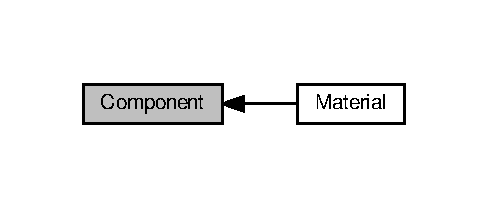
\includegraphics[width=234pt]{group___component}
\end{center}
\end{figure}
\subsection*{Modules}
\begin{DoxyCompactItemize}
\item 
\hyperlink{group___material}{Material}
\end{DoxyCompactItemize}


\subsection{Detailed Description}

\hypertarget{group___material}{}\section{Material}
\label{group___material}\index{Material@{Material}}
Collaboration diagram for Material\+:\nopagebreak
\begin{figure}[H]
\begin{center}
\leavevmode
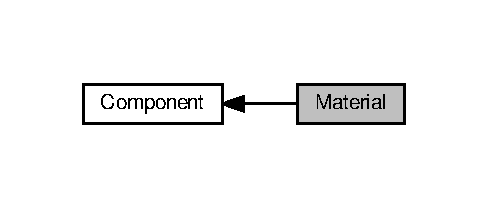
\includegraphics[width=234pt]{group___material}
\end{center}
\end{figure}
\subsection*{Classes}
\begin{DoxyCompactItemize}
\item 
class \hyperlink{class_hlms_terrain}{Hlms\+Terrain}
\item 
struct \hyperlink{struct_terrain_property}{Terrain\+Property}
\end{DoxyCompactItemize}


\subsection{Detailed Description}

\hypertarget{group___core}{}\section{Core}
\label{group___core}\index{Core@{Core}}
Collaboration diagram for Core\+:\nopagebreak
\begin{figure}[H]
\begin{center}
\leavevmode
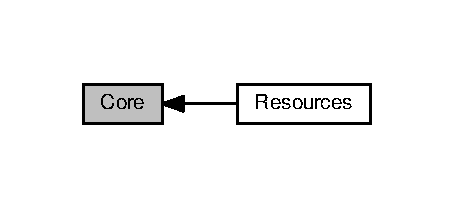
\includegraphics[width=218pt]{group___core}
\end{center}
\end{figure}
\subsection*{Modules}
\begin{DoxyCompactItemize}
\item 
\hyperlink{group___resources}{Resources}
\end{DoxyCompactItemize}


\subsection{Detailed Description}

\hypertarget{group___resources}{}\section{Resources}
\label{group___resources}\index{Resources@{Resources}}
Collaboration diagram for Resources\+:\nopagebreak
\begin{figure}[H]
\begin{center}
\leavevmode
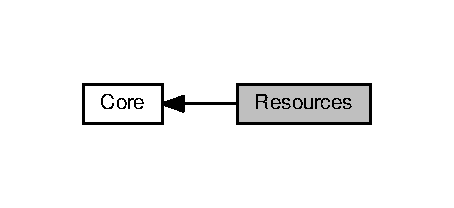
\includegraphics[width=218pt]{group___resources}
\end{center}
\end{figure}
\subsection*{Classes}
\begin{DoxyCompactItemize}
\item 
struct \hyperlink{struct_packed_texture}{Packed\+Texture}
\item 
struct \hyperlink{struct_terrain_baked_texture}{Terrain\+Baked\+Texture}
\item 
class \hyperlink{class_hlms_terrain_datablock}{Hlms\+Terrain\+Datablock}
\end{DoxyCompactItemize}
\subsection*{Typedefs}
\begin{DoxyCompactItemize}
\item 
\mbox{\Hypertarget{group___resources_ga3acc3af61a63f13c587deeb475f10b2e}\label{group___resources_ga3acc3af61a63f13c587deeb475f10b2e}} 
typedef Ogre\+::\+Fast\+Array$<$ \hyperlink{struct_terrain_baked_texture}{Terrain\+Baked\+Texture} $>$ {\bfseries Terrain\+Baked\+Texture\+Array}
\end{DoxyCompactItemize}


\subsection{Detailed Description}

\chapter{Class Documentation}
\hypertarget{class_common_1_1_base_system}{}\section{Common\+:\+:Base\+System Class Reference}
\label{class_common_1_1_base_system}\index{Common\+::\+Base\+System@{Common\+::\+Base\+System}}


Simple System implementing basic functions.  




{\ttfamily \#include $<$Base\+System.\+h$>$}



Inheritance diagram for Common\+:\+:Base\+System\+:\nopagebreak
\begin{figure}[H]
\begin{center}
\leavevmode
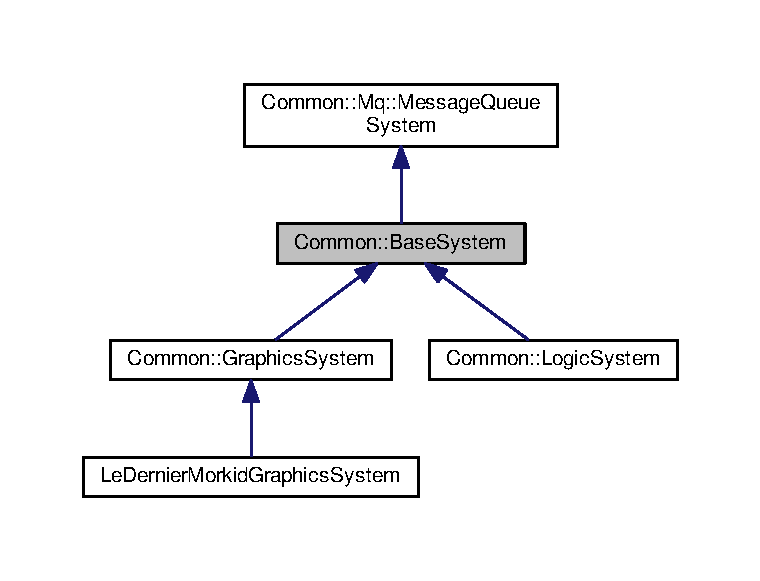
\includegraphics[width=350pt]{class_common_1_1_base_system__inherit__graph}
\end{center}
\end{figure}


Collaboration diagram for Common\+:\+:Base\+System\+:\nopagebreak
\begin{figure}[H]
\begin{center}
\leavevmode
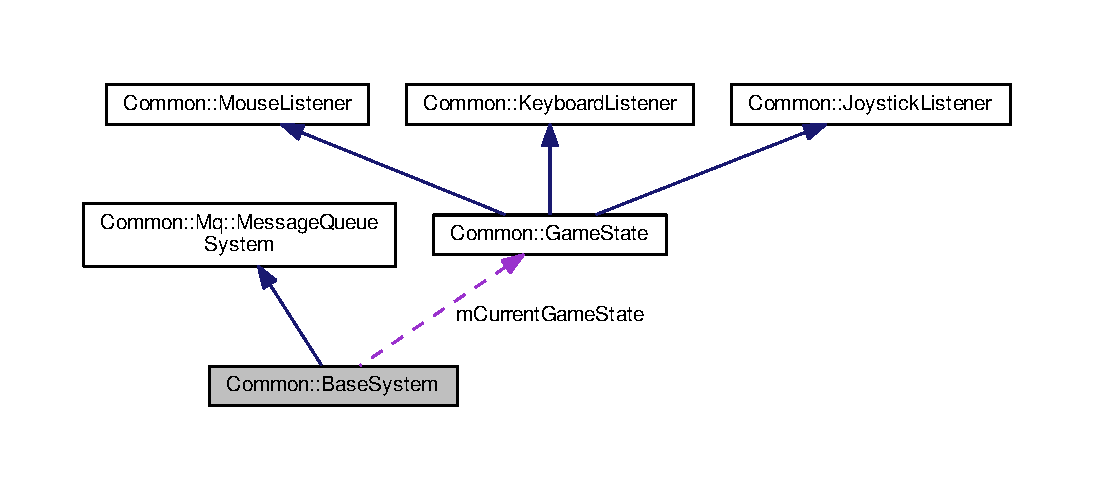
\includegraphics[width=350pt]{class_common_1_1_base_system__coll__graph}
\end{center}
\end{figure}
\subsection*{Public Member Functions}
\begin{DoxyCompactItemize}
\item 
\hyperlink{class_common_1_1_base_system_a420a9f2bb9ccec58af8de74cfc71a9fd}{Base\+System} (\hyperlink{class_common_1_1_game_state}{Game\+State} $\ast$game\+State)
\item 
\mbox{\Hypertarget{class_common_1_1_base_system_a90dcca3acf8e4a37aa0036125ec6b830}\label{class_common_1_1_base_system_a90dcca3acf8e4a37aa0036125ec6b830}} 
virtual \hyperlink{class_common_1_1_base_system_a90dcca3acf8e4a37aa0036125ec6b830}{$\sim$\+Base\+System} ()
\begin{DoxyCompactList}\small\item\em Simple Destructor. \end{DoxyCompactList}\item 
virtual void \hyperlink{class_common_1_1_base_system_a84f42ac8703c9121f29e341070a26c4f}{initialize} (void)
\item 
virtual void \hyperlink{class_common_1_1_base_system_a081f0d3daaff552efe736e6096d329e9}{deinitialize} (void)
\item 
virtual void \hyperlink{class_common_1_1_base_system_a1f26fc7376152a90de585fd50c396427}{create\+Scene} (void)
\item 
virtual void \hyperlink{class_common_1_1_base_system_a04ce870b4d3429942afb58137fd376ca}{destroy\+Scene} (void)
\item 
\mbox{\Hypertarget{class_common_1_1_base_system_a631f234a7a0e46e9f6476520cd2f9bab}\label{class_common_1_1_base_system_a631f234a7a0e46e9f6476520cd2f9bab}} 
void \hyperlink{class_common_1_1_base_system_a631f234a7a0e46e9f6476520cd2f9bab}{begin\+Frame\+Parallel} (void)
\begin{DoxyCompactList}\small\item\em Method to call at the beginning of the Frame. \end{DoxyCompactList}\item 
void \hyperlink{class_common_1_1_base_system_af71a7156da8b0a4feab83ad72162a0c2}{update} (float time\+Since\+Last)
\item 
\mbox{\Hypertarget{class_common_1_1_base_system_a50d9e0044a1cc4b400b847c923913d81}\label{class_common_1_1_base_system_a50d9e0044a1cc4b400b847c923913d81}} 
void \hyperlink{class_common_1_1_base_system_a50d9e0044a1cc4b400b847c923913d81}{finish\+Frame\+Parallel} (void)
\begin{DoxyCompactList}\small\item\em Method to call at the end of the frame. \end{DoxyCompactList}\item 
\mbox{\Hypertarget{class_common_1_1_base_system_ad8d31cde53383edccb40c3b986252f1c}\label{class_common_1_1_base_system_ad8d31cde53383edccb40c3b986252f1c}} 
void \hyperlink{class_common_1_1_base_system_ad8d31cde53383edccb40c3b986252f1c}{finish\+Frame} (void)
\begin{DoxyCompactList}\small\item\em Method to call at the end of the frame. \end{DoxyCompactList}\item 
void \hyperlink{class_common_1_1_base_system_a6820dfed1ee63f376e5773b361e3d2a8}{process\+Incoming\+Message} (\hyperlink{group___common_gaa8c87d2b450282716c906da283e149e6}{Mq\+::\+Message\+Id} message\+Id, const void $\ast$data)
\end{DoxyCompactItemize}
\subsection*{Protected Attributes}
\begin{DoxyCompactItemize}
\item 
\hyperlink{class_common_1_1_game_state}{Game\+State} $\ast$ \hyperlink{class_common_1_1_base_system_a18e8e37eb4089bbde95459e16291b87a}{m\+Current\+Game\+State}
\begin{DoxyCompactList}\small\item\em Current \hyperlink{class_common_1_1_game_state}{Game\+State} to which is transmitted the events. \end{DoxyCompactList}\end{DoxyCompactItemize}
\subsection*{Additional Inherited Members}


\subsection{Detailed Description}
Simple System implementing basic functions. 

\begin{DoxyRemark}{Remarks}
This class is not useful without inheritance, you should implement it to fit with your expectations 
\end{DoxyRemark}
\begin{DoxySeeAlso}{See also}
\hyperlink{class_common_1_1_graphics_system}{Graphics\+System}, \hyperlink{class_common_1_1_logic_system}{Logic\+System} 
\end{DoxySeeAlso}


Definition at line 19 of file Base\+System.\+h.



\subsection{Constructor \& Destructor Documentation}
\mbox{\Hypertarget{class_common_1_1_base_system_a420a9f2bb9ccec58af8de74cfc71a9fd}\label{class_common_1_1_base_system_a420a9f2bb9ccec58af8de74cfc71a9fd}} 
\index{Common\+::\+Base\+System@{Common\+::\+Base\+System}!Base\+System@{Base\+System}}
\index{Base\+System@{Base\+System}!Common\+::\+Base\+System@{Common\+::\+Base\+System}}
\subsubsection{\texorpdfstring{Base\+System()}{BaseSystem()}}
{\footnotesize\ttfamily Common\+::\+Base\+System\+::\+Base\+System (\begin{DoxyParamCaption}\item[{\hyperlink{class_common_1_1_game_state}{Game\+State} $\ast$}]{game\+State }\end{DoxyParamCaption})}

Constructor of \hyperlink{class_common_1_1_base_system}{Base\+System} 
\begin{DoxyParams}{Parameters}
{\em game\+State} & \hyperlink{class_common_1_1_game_state}{Game\+State} to which transmit the events \\
\hline
\end{DoxyParams}


Definition at line 7 of file Base\+System.\+cpp.



\subsection{Member Function Documentation}
\mbox{\Hypertarget{class_common_1_1_base_system_a1f26fc7376152a90de585fd50c396427}\label{class_common_1_1_base_system_a1f26fc7376152a90de585fd50c396427}} 
\index{Common\+::\+Base\+System@{Common\+::\+Base\+System}!create\+Scene@{create\+Scene}}
\index{create\+Scene@{create\+Scene}!Common\+::\+Base\+System@{Common\+::\+Base\+System}}
\subsubsection{\texorpdfstring{create\+Scene()}{createScene()}}
{\footnotesize\ttfamily void Common\+::\+Base\+System\+::create\+Scene (\begin{DoxyParamCaption}\item[{void}]{ }\end{DoxyParamCaption})\hspace{0.3cm}{\ttfamily [virtual]}}

Create the Scene through \hyperlink{class_common_1_1_game_state_a30b77d03dd849ebb2d6698686e9e7619}{Game\+State\+::create\+Scene} \begin{DoxySeeAlso}{See also}
\hyperlink{class_common_1_1_game_state_a30b77d03dd849ebb2d6698686e9e7619}{Game\+State\+::create\+Scene} 
\end{DoxySeeAlso}


Definition at line 16 of file Base\+System.\+cpp.

\mbox{\Hypertarget{class_common_1_1_base_system_a081f0d3daaff552efe736e6096d329e9}\label{class_common_1_1_base_system_a081f0d3daaff552efe736e6096d329e9}} 
\index{Common\+::\+Base\+System@{Common\+::\+Base\+System}!deinitialize@{deinitialize}}
\index{deinitialize@{deinitialize}!Common\+::\+Base\+System@{Common\+::\+Base\+System}}
\subsubsection{\texorpdfstring{deinitialize()}{deinitialize()}}
{\footnotesize\ttfamily void Common\+::\+Base\+System\+::deinitialize (\begin{DoxyParamCaption}\item[{void}]{ }\end{DoxyParamCaption})\hspace{0.3cm}{\ttfamily [virtual]}}

Deinitialize the System \begin{DoxySeeAlso}{See also}
Game\+State\+::uninitialize 
\end{DoxySeeAlso}


Reimplemented in \hyperlink{class_common_1_1_graphics_system_ade2d4efd6e535d312818a92230eb7dcf}{Common\+::\+Graphics\+System}.



Definition at line 14 of file Base\+System.\+cpp.

\mbox{\Hypertarget{class_common_1_1_base_system_a04ce870b4d3429942afb58137fd376ca}\label{class_common_1_1_base_system_a04ce870b4d3429942afb58137fd376ca}} 
\index{Common\+::\+Base\+System@{Common\+::\+Base\+System}!destroy\+Scene@{destroy\+Scene}}
\index{destroy\+Scene@{destroy\+Scene}!Common\+::\+Base\+System@{Common\+::\+Base\+System}}
\subsubsection{\texorpdfstring{destroy\+Scene()}{destroyScene()}}
{\footnotesize\ttfamily void Common\+::\+Base\+System\+::destroy\+Scene (\begin{DoxyParamCaption}\item[{void}]{ }\end{DoxyParamCaption})\hspace{0.3cm}{\ttfamily [virtual]}}

Destroy the Scene through \hyperlink{class_common_1_1_game_state_a03176055b9cb064b2cea5b64cbf6647a}{Game\+State\+::destroy\+Scene} \begin{DoxySeeAlso}{See also}
\hyperlink{class_common_1_1_game_state_a03176055b9cb064b2cea5b64cbf6647a}{Game\+State\+::destroy\+Scene} 
\end{DoxySeeAlso}


Definition at line 18 of file Base\+System.\+cpp.

\mbox{\Hypertarget{class_common_1_1_base_system_a84f42ac8703c9121f29e341070a26c4f}\label{class_common_1_1_base_system_a84f42ac8703c9121f29e341070a26c4f}} 
\index{Common\+::\+Base\+System@{Common\+::\+Base\+System}!initialize@{initialize}}
\index{initialize@{initialize}!Common\+::\+Base\+System@{Common\+::\+Base\+System}}
\subsubsection{\texorpdfstring{initialize()}{initialize()}}
{\footnotesize\ttfamily void Common\+::\+Base\+System\+::initialize (\begin{DoxyParamCaption}\item[{void}]{ }\end{DoxyParamCaption})\hspace{0.3cm}{\ttfamily [virtual]}}

Initialize the System \begin{DoxySeeAlso}{See also}
\hyperlink{class_common_1_1_game_state_a4e7fa2fbc9080111213ce379eb33d082}{Game\+State\+::initialize} 
\end{DoxySeeAlso}


Reimplemented in \hyperlink{class_common_1_1_logic_system_a6e1389a1e2ed8dd21b46fabdedee5d22}{Common\+::\+Logic\+System}.



Definition at line 12 of file Base\+System.\+cpp.

\mbox{\Hypertarget{class_common_1_1_base_system_a6820dfed1ee63f376e5773b361e3d2a8}\label{class_common_1_1_base_system_a6820dfed1ee63f376e5773b361e3d2a8}} 
\index{Common\+::\+Base\+System@{Common\+::\+Base\+System}!process\+Incoming\+Message@{process\+Incoming\+Message}}
\index{process\+Incoming\+Message@{process\+Incoming\+Message}!Common\+::\+Base\+System@{Common\+::\+Base\+System}}
\subsubsection{\texorpdfstring{process\+Incoming\+Message()}{processIncomingMessage()}}
{\footnotesize\ttfamily void Common\+::\+Base\+System\+::process\+Incoming\+Message (\begin{DoxyParamCaption}\item[{\hyperlink{group___common_gaa8c87d2b450282716c906da283e149e6}{Mq\+::\+Message\+Id}}]{message\+Id,  }\item[{const void $\ast$}]{data }\end{DoxyParamCaption})\hspace{0.3cm}{\ttfamily [virtual]}}

Process received messages 
\begin{DoxyParams}{Parameters}
{\em message\+Id} & The Mq\+::\+Message\+Id of the message, used to know what kind of message it is \\
\hline
{\em data} & The data sent with the message, could be anything. Depending on the message\+Id, a conversion will be needed \\
\hline
\end{DoxyParams}
\begin{DoxySeeAlso}{See also}
\hyperlink{class_common_1_1_mq_1_1_message_queue_system_ad6eb849b72f03e3e4f09c6457c8ecda6}{Common\+::\+Mq\+::\+Message\+Queue\+System\+::process\+Incoming\+Message} 
\end{DoxySeeAlso}


Implements \hyperlink{class_common_1_1_mq_1_1_message_queue_system_ad6eb849b72f03e3e4f09c6457c8ecda6}{Common\+::\+Mq\+::\+Message\+Queue\+System}.



Reimplemented in \hyperlink{class_common_1_1_graphics_system_a8d286a151ed9a65f0eebe1ac119e2d59}{Common\+::\+Graphics\+System}, and \hyperlink{class_common_1_1_logic_system_a4495ecadf034103ad58deab6802543fa}{Common\+::\+Logic\+System}.



Definition at line 32 of file Base\+System.\+cpp.

\mbox{\Hypertarget{class_common_1_1_base_system_af71a7156da8b0a4feab83ad72162a0c2}\label{class_common_1_1_base_system_af71a7156da8b0a4feab83ad72162a0c2}} 
\index{Common\+::\+Base\+System@{Common\+::\+Base\+System}!update@{update}}
\index{update@{update}!Common\+::\+Base\+System@{Common\+::\+Base\+System}}
\subsubsection{\texorpdfstring{update()}{update()}}
{\footnotesize\ttfamily void Common\+::\+Base\+System\+::update (\begin{DoxyParamCaption}\item[{float}]{time\+Since\+Last }\end{DoxyParamCaption})}

Method to update the System. Call it one time per frame 
\begin{DoxyParams}{Parameters}
{\em time\+Since\+Last} & Time since the last frame \\
\hline
\end{DoxyParams}


Definition at line 22 of file Base\+System.\+cpp.



\subsection{Member Data Documentation}
\mbox{\Hypertarget{class_common_1_1_base_system_a18e8e37eb4089bbde95459e16291b87a}\label{class_common_1_1_base_system_a18e8e37eb4089bbde95459e16291b87a}} 
\index{Common\+::\+Base\+System@{Common\+::\+Base\+System}!m\+Current\+Game\+State@{m\+Current\+Game\+State}}
\index{m\+Current\+Game\+State@{m\+Current\+Game\+State}!Common\+::\+Base\+System@{Common\+::\+Base\+System}}
\subsubsection{\texorpdfstring{m\+Current\+Game\+State}{mCurrentGameState}}
{\footnotesize\ttfamily Common\+::\+Base\+System\+::m\+Current\+Game\+State\hspace{0.3cm}{\ttfamily [protected]}}



Current \hyperlink{class_common_1_1_game_state}{Game\+State} to which is transmitted the events. 

\begin{DoxySeeAlso}{See also}
\hyperlink{class_common_1_1_base_system_a420a9f2bb9ccec58af8de74cfc71a9fd}{Base\+System\+::\+Base\+System} 
\end{DoxySeeAlso}


Definition at line 28 of file Base\+System.\+h.



The documentation for this class was generated from the following files\+:\begin{DoxyCompactItemize}
\item 
/home/louis/projects/\+Le\+Dernier\+Morkid/\+Common/include/Base\+System.\+h\item 
/home/louis/projects/\+Le\+Dernier\+Morkid/\+Common/src/Base\+System.\+cpp\end{DoxyCompactItemize}

\hypertarget{class_common_1_1_camera_controller}{}\section{Common\+:\+:Camera\+Controller Class Reference}
\label{class_common_1_1_camera_controller}\index{Common\+::\+Camera\+Controller@{Common\+::\+Camera\+Controller}}


Inheritance diagram for Common\+:\+:Camera\+Controller\+:\nopagebreak
\begin{figure}[H]
\begin{center}
\leavevmode
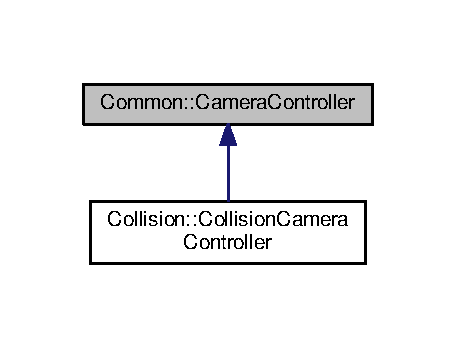
\includegraphics[width=219pt]{class_common_1_1_camera_controller__inherit__graph}
\end{center}
\end{figure}


Collaboration diagram for Common\+:\+:Camera\+Controller\+:\nopagebreak
\begin{figure}[H]
\begin{center}
\leavevmode
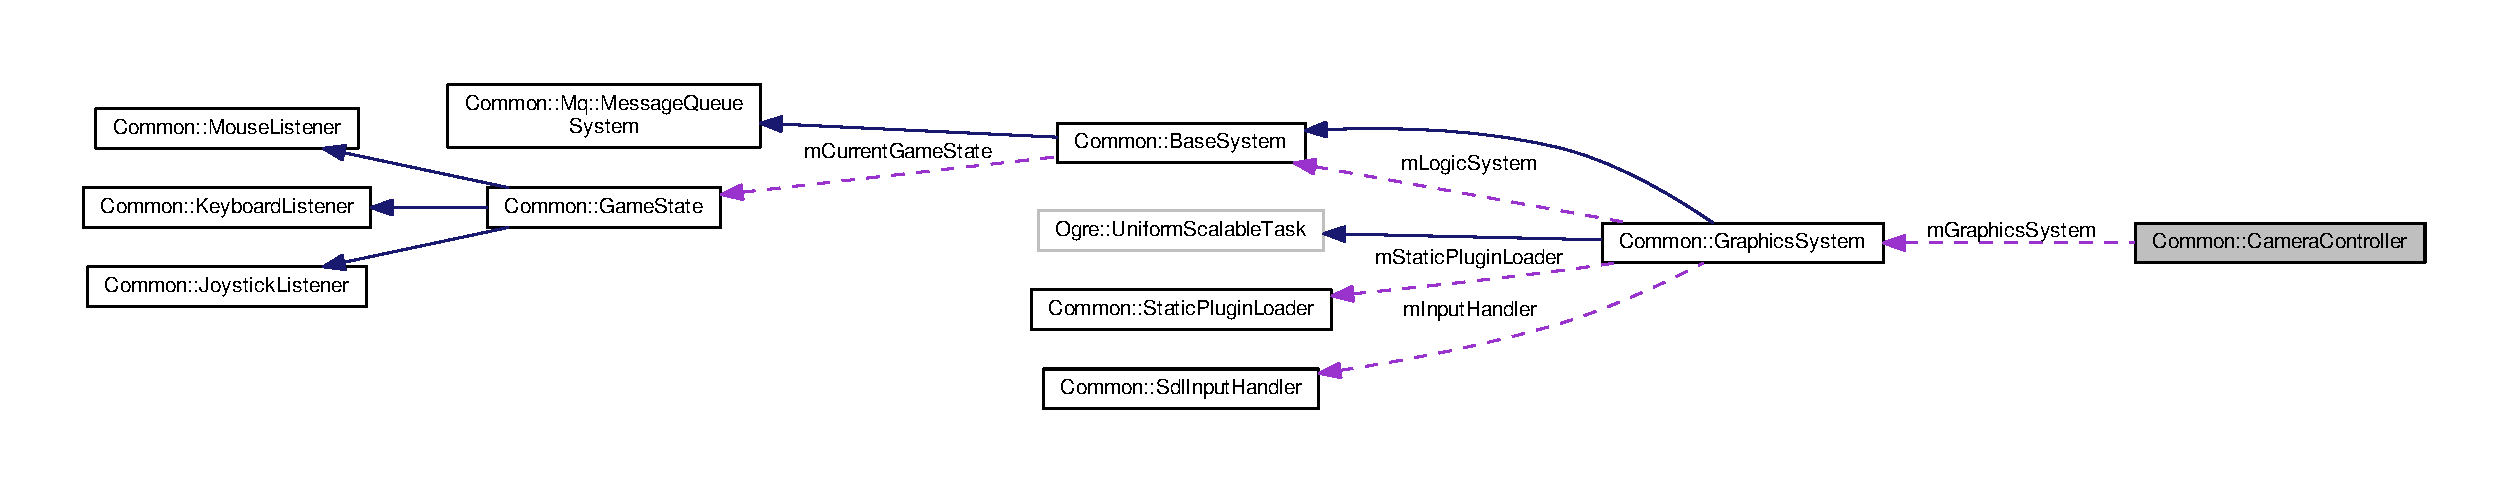
\includegraphics[width=350pt]{class_common_1_1_camera_controller__coll__graph}
\end{center}
\end{figure}
\subsection*{Public Member Functions}
\begin{DoxyCompactItemize}
\item 
\mbox{\Hypertarget{class_common_1_1_camera_controller_a09c9f866ac2161de31ff45694dd711fd}\label{class_common_1_1_camera_controller_a09c9f866ac2161de31ff45694dd711fd}} 
{\bfseries Camera\+Controller} (\hyperlink{class_common_1_1_graphics_system}{Graphics\+System} $\ast$graphics\+System, bool use\+Scene\+Node=false)
\item 
\mbox{\Hypertarget{class_common_1_1_camera_controller_a5d11cbced7f78eec997b96bb489d0806}\label{class_common_1_1_camera_controller_a5d11cbced7f78eec997b96bb489d0806}} 
virtual void {\bfseries update} (float time\+Since\+Last)
\item 
\mbox{\Hypertarget{class_common_1_1_camera_controller_aefb0839a3f45e4390c764762b7a053a1}\label{class_common_1_1_camera_controller_aefb0839a3f45e4390c764762b7a053a1}} 
virtual bool \hyperlink{class_common_1_1_camera_controller_aefb0839a3f45e4390c764762b7a053a1}{key\+Pressed} (const \hyperlink{struct_s_d_l___keyboard_event}{S\+D\+L\+\_\+\+Keyboard\+Event} \&arg)
\begin{DoxyCompactList}\small\item\em Returns true if we\textquotesingle{}ve handled the event. \end{DoxyCompactList}\item 
\mbox{\Hypertarget{class_common_1_1_camera_controller_a2ade17644b5c6a9249b6fcff6c358b2e}\label{class_common_1_1_camera_controller_a2ade17644b5c6a9249b6fcff6c358b2e}} 
virtual bool \hyperlink{class_common_1_1_camera_controller_a2ade17644b5c6a9249b6fcff6c358b2e}{key\+Released} (const \hyperlink{struct_s_d_l___keyboard_event}{S\+D\+L\+\_\+\+Keyboard\+Event} \&arg)
\begin{DoxyCompactList}\small\item\em Returns true if we\textquotesingle{}ve handled the event. \end{DoxyCompactList}\item 
\mbox{\Hypertarget{class_common_1_1_camera_controller_af56a45fb24b5c2e5603210be8377aa8d}\label{class_common_1_1_camera_controller_af56a45fb24b5c2e5603210be8377aa8d}} 
virtual void {\bfseries mouse\+Moved} (const \hyperlink{union_s_d_l___event}{S\+D\+L\+\_\+\+Event} \&arg)
\end{DoxyCompactItemize}
\subsection*{Public Attributes}
\begin{DoxyCompactItemize}
\item 
\mbox{\Hypertarget{class_common_1_1_camera_controller_a89119788b0320e34bd0322006bbd9734}\label{class_common_1_1_camera_controller_a89119788b0320e34bd0322006bbd9734}} 
float {\bfseries m\+Camera\+Base\+Speed}
\item 
\mbox{\Hypertarget{class_common_1_1_camera_controller_a043ce9247c01a9cc852b7e58e0b46e06}\label{class_common_1_1_camera_controller_a043ce9247c01a9cc852b7e58e0b46e06}} 
float {\bfseries m\+Camera\+Speed\+Boost}
\end{DoxyCompactItemize}
\subsection*{Protected Types}
\begin{DoxyCompactItemize}
\item 
\mbox{\Hypertarget{class_common_1_1_camera_controller_af299b39b39b578b2235220e5fa8dfc01}\label{class_common_1_1_camera_controller_af299b39b39b578b2235220e5fa8dfc01}} 
enum {\bfseries Action} \{ \newline
{\bfseries Forward}, 
{\bfseries Backward}, 
{\bfseries Leftward}, 
{\bfseries Rightward}, 
\newline
{\bfseries Up}, 
{\bfseries Down}, 
{\bfseries Run}
 \}
\item 
\mbox{\Hypertarget{class_common_1_1_camera_controller_a75aa76cde460aabcb220ca664f3d40a1}\label{class_common_1_1_camera_controller_a75aa76cde460aabcb220ca664f3d40a1}} 
typedef std\+::pair$<$ S\+D\+L\+\_\+\+Keycode, bool $>$ {\bfseries Key\+State}
\item 
\mbox{\Hypertarget{class_common_1_1_camera_controller_a33ec61812e24b2f120a08127435c52dc}\label{class_common_1_1_camera_controller_a33ec61812e24b2f120a08127435c52dc}} 
typedef std\+::map$<$ Action, Key\+State $>$ {\bfseries Keymap\+State}
\end{DoxyCompactItemize}
\subsection*{Protected Attributes}
\begin{DoxyCompactItemize}
\item 
\mbox{\Hypertarget{class_common_1_1_camera_controller_aa2db4d904aadf4af7f663e6385fa1a7e}\label{class_common_1_1_camera_controller_aa2db4d904aadf4af7f663e6385fa1a7e}} 
bool {\bfseries m\+Use\+Scene\+Node}
\item 
\mbox{\Hypertarget{class_common_1_1_camera_controller_a074c334b4156cf5b7c334e41b7e34619}\label{class_common_1_1_camera_controller_a074c334b4156cf5b7c334e41b7e34619}} 
bool {\bfseries m\+Use\+Collision}
\item 
\mbox{\Hypertarget{class_common_1_1_camera_controller_a3652121296a21279131ce9197ea57995}\label{class_common_1_1_camera_controller_a3652121296a21279131ce9197ea57995}} 
bool {\bfseries m\+Speed\+Modifier}
\item 
\mbox{\Hypertarget{class_common_1_1_camera_controller_a6de401fd5501b9f48aab9efc11e5da68}\label{class_common_1_1_camera_controller_a6de401fd5501b9f48aab9efc11e5da68}} 
Keymap\+State {\bfseries m\+Keymap\+State}
\item 
\mbox{\Hypertarget{class_common_1_1_camera_controller_af0c031abefd0e2caebdc18795d1953df}\label{class_common_1_1_camera_controller_af0c031abefd0e2caebdc18795d1953df}} 
float {\bfseries m\+Camera\+Yaw}
\item 
\mbox{\Hypertarget{class_common_1_1_camera_controller_a53ffb8220c31ac47f8c7c336a4bebe62}\label{class_common_1_1_camera_controller_a53ffb8220c31ac47f8c7c336a4bebe62}} 
float {\bfseries m\+Camera\+Pitch}
\item 
\mbox{\Hypertarget{class_common_1_1_camera_controller_ae2970e63d46f18b24b8a0ae4b6acf247}\label{class_common_1_1_camera_controller_ae2970e63d46f18b24b8a0ae4b6acf247}} 
\hyperlink{class_common_1_1_graphics_system}{Graphics\+System} $\ast$ {\bfseries m\+Graphics\+System}
\end{DoxyCompactItemize}


The documentation for this class was generated from the following files\+:\begin{DoxyCompactItemize}
\item 
/home/louis/projects/\+Le\+Dernier\+Morkid/\+Common/include/Camera\+Controller.\+h\item 
/home/louis/projects/\+Le\+Dernier\+Morkid/\+Common/src/Camera\+Controller.\+cpp\end{DoxyCompactItemize}

\hypertarget{class_collision_1_1_collision_camera_controller}{}\section{Collision\+:\+:Collision\+Camera\+Controller Class Reference}
\label{class_collision_1_1_collision_camera_controller}\index{Collision\+::\+Collision\+Camera\+Controller@{Collision\+::\+Collision\+Camera\+Controller}}


Camera Controller using Collision.  




{\ttfamily \#include $<$Collision\+Camera\+Controller.\+h$>$}



Inheritance diagram for Collision\+:\+:Collision\+Camera\+Controller\+:\nopagebreak
\begin{figure}[H]
\begin{center}
\leavevmode
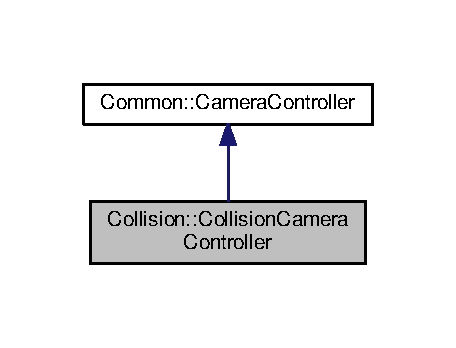
\includegraphics[width=219pt]{class_collision_1_1_collision_camera_controller__inherit__graph}
\end{center}
\end{figure}


Collaboration diagram for Collision\+:\+:Collision\+Camera\+Controller\+:\nopagebreak
\begin{figure}[H]
\begin{center}
\leavevmode
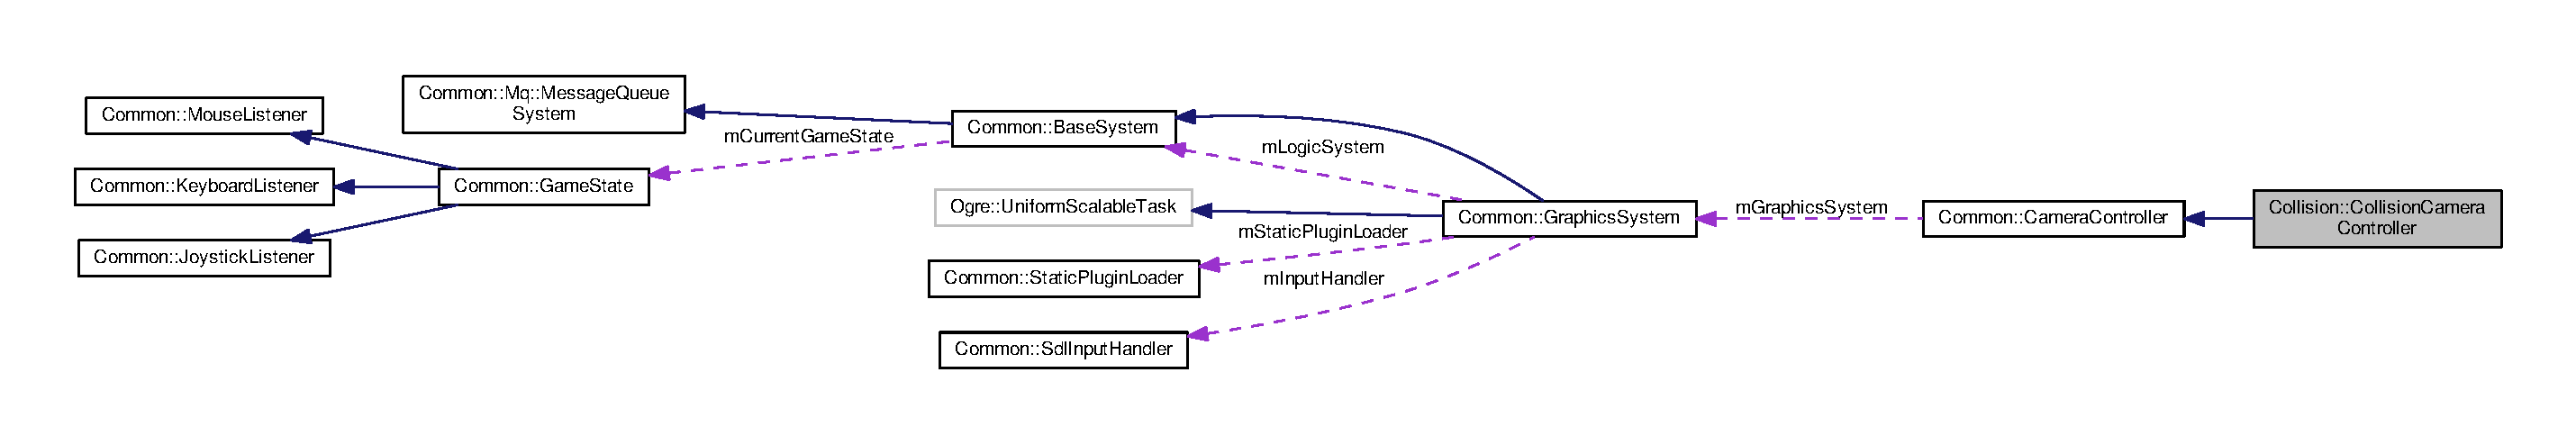
\includegraphics[width=350pt]{class_collision_1_1_collision_camera_controller__coll__graph}
\end{center}
\end{figure}
\subsection*{Public Member Functions}
\begin{DoxyCompactItemize}
\item 
\hyperlink{class_collision_1_1_collision_camera_controller_ac22915566c34afa0c50400e26dcb667b}{Collision\+Camera\+Controller} (\hyperlink{class_common_1_1_graphics_system}{Common\+::\+Graphics\+System} $\ast$graphics\+System, bt\+Dynamics\+World $\ast$world)
\item 
virtual void \hyperlink{class_collision_1_1_collision_camera_controller_ac25037b29b022a2ccf77b16fe0bda670}{update} (float time\+Since\+Last)
\end{DoxyCompactItemize}
\subsection*{Private Attributes}
\begin{DoxyCompactItemize}
\item 
\mbox{\Hypertarget{class_collision_1_1_collision_camera_controller_a63cbe384f546c982ea24bbe8918a07d4}\label{class_collision_1_1_collision_camera_controller_a63cbe384f546c982ea24bbe8918a07d4}} 
bt\+Dynamics\+World $\ast$ \hyperlink{class_collision_1_1_collision_camera_controller_a63cbe384f546c982ea24bbe8918a07d4}{m\+World}
\begin{DoxyCompactList}\small\item\em bt\+Dynamics\+World in which the Camera evolve \end{DoxyCompactList}\item 
\mbox{\Hypertarget{class_collision_1_1_collision_camera_controller_a6f4788c90fef7434302dec9d78e2e87c}\label{class_collision_1_1_collision_camera_controller_a6f4788c90fef7434302dec9d78e2e87c}} 
bt\+Pair\+Caching\+Ghost\+Object $\ast$ \hyperlink{class_collision_1_1_collision_camera_controller_a6f4788c90fef7434302dec9d78e2e87c}{m\+Ghost\+Object}
\begin{DoxyCompactList}\small\item\em Attribute which provide collision to the Camera. \end{DoxyCompactList}\item 
\mbox{\Hypertarget{class_collision_1_1_collision_camera_controller_aeeb0d5cda4e63c73aeda6cf87e5b4b3d}\label{class_collision_1_1_collision_camera_controller_aeeb0d5cda4e63c73aeda6cf87e5b4b3d}} 
bt\+Kinematic\+Character\+Controller $\ast$ \hyperlink{class_collision_1_1_collision_camera_controller_aeeb0d5cda4e63c73aeda6cf87e5b4b3d}{m\+Character}
\begin{DoxyCompactList}\small\item\em Kinematic Object used to control m\+Ghost\+Object. \end{DoxyCompactList}\end{DoxyCompactItemize}
\subsection*{Additional Inherited Members}


\subsection{Detailed Description}
Camera Controller using Collision. 

Camera Controller using bt\+Ghost\+Object and bt\+Kinematic\+Character\+Controller to move the Camera 

Definition at line 15 of file Collision\+Camera\+Controller.\+h.



\subsection{Constructor \& Destructor Documentation}
\mbox{\Hypertarget{class_collision_1_1_collision_camera_controller_ac22915566c34afa0c50400e26dcb667b}\label{class_collision_1_1_collision_camera_controller_ac22915566c34afa0c50400e26dcb667b}} 
\index{Collision\+::\+Collision\+Camera\+Controller@{Collision\+::\+Collision\+Camera\+Controller}!Collision\+Camera\+Controller@{Collision\+Camera\+Controller}}
\index{Collision\+Camera\+Controller@{Collision\+Camera\+Controller}!Collision\+::\+Collision\+Camera\+Controller@{Collision\+::\+Collision\+Camera\+Controller}}
\subsubsection{\texorpdfstring{Collision\+Camera\+Controller()}{CollisionCameraController()}}
{\footnotesize\ttfamily Collision\+::\+Collision\+Camera\+Controller\+::\+Collision\+Camera\+Controller (\begin{DoxyParamCaption}\item[{\hyperlink{class_common_1_1_graphics_system}{Common\+::\+Graphics\+System} $\ast$}]{graphics\+System,  }\item[{bt\+Dynamics\+World $\ast$}]{world }\end{DoxyParamCaption})}

Constructor of \hyperlink{class_collision_1_1_collision_camera_controller}{Collision\+Camera\+Controller} 
\begin{DoxyParams}{Parameters}
{\em graphics\+System} & The \hyperlink{class_common_1_1_graphics_system}{Common\+::\+Graphics\+System} which owned the camera \\
\hline
{\em world} & The World in which the \hyperlink{class_collision_1_1_collision_camera_controller}{Collision\+Camera\+Controller} will evolve \\
\hline
\end{DoxyParams}


Definition at line 13 of file Collision\+Camera\+Controller.\+cpp.



\subsection{Member Function Documentation}
\mbox{\Hypertarget{class_collision_1_1_collision_camera_controller_ac25037b29b022a2ccf77b16fe0bda670}\label{class_collision_1_1_collision_camera_controller_ac25037b29b022a2ccf77b16fe0bda670}} 
\index{Collision\+::\+Collision\+Camera\+Controller@{Collision\+::\+Collision\+Camera\+Controller}!update@{update}}
\index{update@{update}!Collision\+::\+Collision\+Camera\+Controller@{Collision\+::\+Collision\+Camera\+Controller}}
\subsubsection{\texorpdfstring{update()}{update()}}
{\footnotesize\ttfamily void Collision\+::\+Collision\+Camera\+Controller\+::update (\begin{DoxyParamCaption}\item[{float}]{time\+Since\+Last }\end{DoxyParamCaption})\hspace{0.3cm}{\ttfamily [virtual]}}

Method called in order to move and rotate the bt\+Ghost\+Object and synchronize the Ogre\+::\+Camera 
\begin{DoxyParams}{Parameters}
{\em time\+Since\+Last} & The time past since last call \\
\hline
\end{DoxyParams}


Reimplemented from \hyperlink{class_common_1_1_camera_controller_a5d11cbced7f78eec997b96bb489d0806}{Common\+::\+Camera\+Controller}.



Definition at line 30 of file Collision\+Camera\+Controller.\+cpp.



The documentation for this class was generated from the following files\+:\begin{DoxyCompactItemize}
\item 
/home/louis/projects/\+Le\+Dernier\+Morkid/\+Collision/include/Collision\+Camera\+Controller.\+h\item 
/home/louis/projects/\+Le\+Dernier\+Morkid/\+Collision/src/Collision\+Camera\+Controller.\+cpp\end{DoxyCompactItemize}

\hypertarget{struct_common_1_1_collision_object_definition}{}\section{Common\+:\+:Collision\+Object\+Definition Struct Reference}
\label{struct_common_1_1_collision_object_definition}\index{Common\+::\+Collision\+Object\+Definition@{Common\+::\+Collision\+Object\+Definition}}
\subsection*{Public Attributes}
\begin{DoxyCompactItemize}
\item 
\mbox{\Hypertarget{struct_common_1_1_collision_object_definition_a472145ada80dba6a8d1831246b0ed2c3}\label{struct_common_1_1_collision_object_definition_a472145ada80dba6a8d1831246b0ed2c3}} 
unsigned int {\bfseries mass}
\item 
\mbox{\Hypertarget{struct_common_1_1_collision_object_definition_a84df96597dafbddce2bd7f8e0a8770a3}\label{struct_common_1_1_collision_object_definition_a84df96597dafbddce2bd7f8e0a8770a3}} 
unsigned int {\bfseries restitution}
\item 
\mbox{\Hypertarget{struct_common_1_1_collision_object_definition_a8cf81893bc2b5cd90861239c9a758c68}\label{struct_common_1_1_collision_object_definition_a8cf81893bc2b5cd90861239c9a758c68}} 
unsigned int {\bfseries friction}
\item 
\mbox{\Hypertarget{struct_common_1_1_collision_object_definition_a9528a6850d27727bc573460430c63cf2}\label{struct_common_1_1_collision_object_definition_a9528a6850d27727bc573460430c63cf2}} 
Collision\+Object\+Type {\bfseries co\+Type}
\item 
\mbox{\Hypertarget{struct_common_1_1_collision_object_definition_a9ce0f0e3eb7b066ee634bcbec7cce193}\label{struct_common_1_1_collision_object_definition_a9ce0f0e3eb7b066ee634bcbec7cce193}} 
bt\+Collision\+Shape $\ast$ {\bfseries shape}
\end{DoxyCompactItemize}


The documentation for this struct was generated from the following file\+:\begin{DoxyCompactItemize}
\item 
/home/louis/projects/\+Le\+Dernier\+Morkid/\+Common/include/Game\+Entity.\+h\end{DoxyCompactItemize}

\hypertarget{class_collision_terrain}{}\section{Collision\+Terrain Class Reference}
\label{class_collision_terrain}\index{Collision\+Terrain@{Collision\+Terrain}}


Inheritance diagram for Collision\+Terrain\+:\nopagebreak
\begin{figure}[H]
\begin{center}
\leavevmode
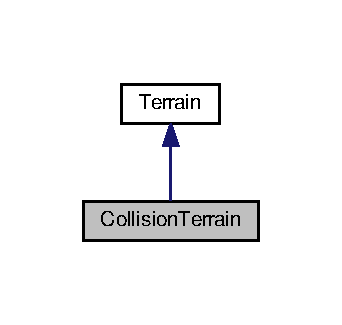
\includegraphics[width=164pt]{class_collision_terrain__inherit__graph}
\end{center}
\end{figure}


Collaboration diagram for Collision\+Terrain\+:\nopagebreak
\begin{figure}[H]
\begin{center}
\leavevmode
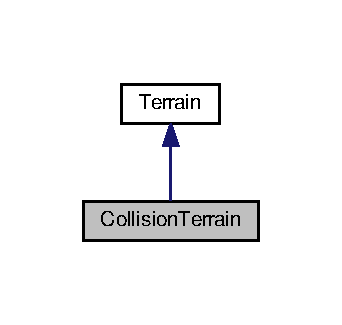
\includegraphics[width=164pt]{class_collision_terrain__coll__graph}
\end{center}
\end{figure}
\subsection*{Public Member Functions}
\begin{DoxyCompactItemize}
\item 
\mbox{\Hypertarget{class_collision_terrain_a078c7bd488c50c875403d6fa6b387ab6}\label{class_collision_terrain_a078c7bd488c50c875403d6fa6b387ab6}} 
{\bfseries Collision\+Terrain} (bt\+Dynamics\+World $\ast$world)
\item 
\mbox{\Hypertarget{class_collision_terrain_a82f5e298e95755e30b873aae483b006d}\label{class_collision_terrain_a82f5e298e95755e30b873aae483b006d}} 
void {\bfseries load} (const Ogre\+::\+String \&tex\+Name, const Ogre\+::\+Vector3 center, const Ogre\+::\+Vector3 \&dimensions)
\end{DoxyCompactItemize}
\subsection*{Protected Member Functions}
\begin{DoxyCompactItemize}
\item 
\mbox{\Hypertarget{class_collision_terrain_a0641937303366dd4576a5ad308513e9b}\label{class_collision_terrain_a0641937303366dd4576a5ad308513e9b}} 
void {\bfseries create\+Shape} ()
\end{DoxyCompactItemize}
\subsection*{Protected Attributes}
\begin{DoxyCompactItemize}
\item 
\mbox{\Hypertarget{class_collision_terrain_a51867cf4e61b0170fdbe81b7b7a84870}\label{class_collision_terrain_a51867cf4e61b0170fdbe81b7b7a84870}} 
bt\+Dynamics\+World $\ast$ {\bfseries m\+World}
\end{DoxyCompactItemize}


\subsection{Detailed Description}


Definition at line 8 of file Collision\+Terrain.\+h.



The documentation for this class was generated from the following files\+:\begin{DoxyCompactItemize}
\item 
/home/louis/projects/\+Le\+Dernier\+Morkid/include/\+Terrain/Collision\+Terrain.\+h\item 
/home/louis/projects/\+Le\+Dernier\+Morkid/src/\+Terrain/Collision\+Terrain.\+cpp\end{DoxyCompactItemize}

\hypertarget{class_collision_1_1_converter}{}\section{Collision\+:\+:Converter Class Reference}
\label{class_collision_1_1_converter}\index{Collision\+::\+Converter@{Collision\+::\+Converter}}


\hyperlink{class_collision_1_1_converter}{Converter} between Bullet to Ogre.  




{\ttfamily \#include $<$Converter.\+h$>$}

\subsection*{Static Public Member Functions}
\begin{DoxyCompactItemize}
\item 
static \hyperlink{struct_common_1_1_game_entity_transform}{Common\+::\+Game\+Entity\+Transform} \hyperlink{class_collision_1_1_converter_a1b08b8571e6e0973029e6eb492cd7888}{to} (const bt\+Transform \&transform, bt\+Vector3 scale=bt\+Vector3(1, 1, 1))
\item 
static bt\+Transform \hyperlink{class_collision_1_1_converter_a532db90a9789b9fdabe21bd5e8f0fcfc}{to} (const \hyperlink{struct_common_1_1_game_entity_transform}{Common\+::\+Game\+Entity\+Transform} \&transform)
\item 
static Ogre\+::\+Quaternion \hyperlink{class_collision_1_1_converter_a303519e4c318cca485ca02399b6a1ed3}{to} (const bt\+Quaternion \&quaternion)
\item 
static bt\+Quaternion \hyperlink{class_collision_1_1_converter_a0ed727c0a2fa4df0409cf0f7e98fe7ce}{to} (const Ogre\+::\+Quaternion \&quaternion)
\item 
static Ogre\+::\+Vector3 \hyperlink{class_collision_1_1_converter_a55c293e2329b62d00c6bd295142b7671}{to} (const bt\+Vector3 \&vector)
\item 
static bt\+Vector3 \hyperlink{class_collision_1_1_converter_a38f61c45f9f05299d3152c729614252c}{to} (const Ogre\+::\+Vector3 \&vector)
\end{DoxyCompactItemize}


\subsection{Detailed Description}
\hyperlink{class_collision_1_1_converter}{Converter} between Bullet to Ogre. 

This class provide functions to convert Ogre Math to Bullet Math (Ogre\+::\+Vector3 -\/$>$ bt\+Vector3 ...) \begin{DoxyRemark}{Remarks}
This class should not be used as an object 
\end{DoxyRemark}


\subsection{Member Function Documentation}
\mbox{\Hypertarget{class_collision_1_1_converter_a1b08b8571e6e0973029e6eb492cd7888}\label{class_collision_1_1_converter_a1b08b8571e6e0973029e6eb492cd7888}} 
\index{Collision\+::\+Converter@{Collision\+::\+Converter}!to@{to}}
\index{to@{to}!Collision\+::\+Converter@{Collision\+::\+Converter}}
\subsubsection{\texorpdfstring{to()}{to()}\hspace{0.1cm}{\footnotesize\ttfamily [1/6]}}
{\footnotesize\ttfamily \hyperlink{struct_common_1_1_game_entity_transform}{Common\+::\+Game\+Entity\+Transform} Collision\+::\+Converter\+::to (\begin{DoxyParamCaption}\item[{const bt\+Transform \&}]{transform,  }\item[{bt\+Vector3}]{scale = {\ttfamily btVector3(1,~1,~1)} }\end{DoxyParamCaption})\hspace{0.3cm}{\ttfamily [static]}}

Convert bt\+Transform to \hyperlink{struct_common_1_1_game_entity_transform}{Common\+::\+Game\+Entity\+Transform} 
\begin{DoxyParams}{Parameters}
{\em transform} & bt\+Transform to convert \\
\hline
{\em scale} & scale to add to transform to create the \hyperlink{struct_common_1_1_game_entity_transform}{Common\+::\+Game\+Entity\+Transform} \\
\hline
\end{DoxyParams}
\begin{DoxyReturn}{Returns}
the \hyperlink{struct_common_1_1_game_entity_transform}{Common\+::\+Game\+Entity\+Transform} created 
\end{DoxyReturn}
\begin{DoxyRemark}{Remarks}
scale is not needed but should not be forgetten, bt\+Transform does not provide scale but \hyperlink{struct_common_1_1_game_entity_transform}{Common\+::\+Game\+Entity\+Transform} does 
\end{DoxyRemark}
\mbox{\Hypertarget{class_collision_1_1_converter_a532db90a9789b9fdabe21bd5e8f0fcfc}\label{class_collision_1_1_converter_a532db90a9789b9fdabe21bd5e8f0fcfc}} 
\index{Collision\+::\+Converter@{Collision\+::\+Converter}!to@{to}}
\index{to@{to}!Collision\+::\+Converter@{Collision\+::\+Converter}}
\subsubsection{\texorpdfstring{to()}{to()}\hspace{0.1cm}{\footnotesize\ttfamily [2/6]}}
{\footnotesize\ttfamily bt\+Transform Collision\+::\+Converter\+::to (\begin{DoxyParamCaption}\item[{const \hyperlink{struct_common_1_1_game_entity_transform}{Common\+::\+Game\+Entity\+Transform} \&}]{transform }\end{DoxyParamCaption})\hspace{0.3cm}{\ttfamily [static]}}

Convert \hyperlink{struct_common_1_1_game_entity_transform}{Common\+::\+Game\+Entity\+Transform} to bt\+Transform 
\begin{DoxyParams}{Parameters}
{\em transform} & \hyperlink{struct_common_1_1_game_entity_transform}{Common\+::\+Game\+Entity\+Transform} to convert \\
\hline
\end{DoxyParams}
\begin{DoxyReturn}{Returns}
the bt\+Transform created 
\end{DoxyReturn}
\begin{DoxyRemark}{Remarks}
As \hyperlink{struct_common_1_1_game_entity_transform}{Common\+::\+Game\+Entity\+Transform} provide a scale attribute but bt\+Transform does not, do not forget to manage this case 
\end{DoxyRemark}
\mbox{\Hypertarget{class_collision_1_1_converter_a303519e4c318cca485ca02399b6a1ed3}\label{class_collision_1_1_converter_a303519e4c318cca485ca02399b6a1ed3}} 
\index{Collision\+::\+Converter@{Collision\+::\+Converter}!to@{to}}
\index{to@{to}!Collision\+::\+Converter@{Collision\+::\+Converter}}
\subsubsection{\texorpdfstring{to()}{to()}\hspace{0.1cm}{\footnotesize\ttfamily [3/6]}}
{\footnotesize\ttfamily Ogre\+::\+Quaternion Collision\+::\+Converter\+::to (\begin{DoxyParamCaption}\item[{const bt\+Quaternion \&}]{quaternion }\end{DoxyParamCaption})\hspace{0.3cm}{\ttfamily [static]}}

Convert bt\+Quaternion to Ogre\+::\+Quaternion 
\begin{DoxyParams}{Parameters}
{\em quaternion} & bt\+Quaternion to convert \\
\hline
\end{DoxyParams}
\begin{DoxyReturn}{Returns}
the Ogre\+::\+Quaternion created 
\end{DoxyReturn}
\mbox{\Hypertarget{class_collision_1_1_converter_a0ed727c0a2fa4df0409cf0f7e98fe7ce}\label{class_collision_1_1_converter_a0ed727c0a2fa4df0409cf0f7e98fe7ce}} 
\index{Collision\+::\+Converter@{Collision\+::\+Converter}!to@{to}}
\index{to@{to}!Collision\+::\+Converter@{Collision\+::\+Converter}}
\subsubsection{\texorpdfstring{to()}{to()}\hspace{0.1cm}{\footnotesize\ttfamily [4/6]}}
{\footnotesize\ttfamily bt\+Quaternion Collision\+::\+Converter\+::to (\begin{DoxyParamCaption}\item[{const Ogre\+::\+Quaternion \&}]{quaternion }\end{DoxyParamCaption})\hspace{0.3cm}{\ttfamily [static]}}

Convert Ogre\+::\+Quaternion to bt\+Quaternion 
\begin{DoxyParams}{Parameters}
{\em quaternion} & Ogre\+::\+Quaternion to convert \\
\hline
\end{DoxyParams}
\begin{DoxyReturn}{Returns}
the bt\+Quaternion created 
\end{DoxyReturn}
\mbox{\Hypertarget{class_collision_1_1_converter_a55c293e2329b62d00c6bd295142b7671}\label{class_collision_1_1_converter_a55c293e2329b62d00c6bd295142b7671}} 
\index{Collision\+::\+Converter@{Collision\+::\+Converter}!to@{to}}
\index{to@{to}!Collision\+::\+Converter@{Collision\+::\+Converter}}
\subsubsection{\texorpdfstring{to()}{to()}\hspace{0.1cm}{\footnotesize\ttfamily [5/6]}}
{\footnotesize\ttfamily Ogre\+::\+Vector3 Collision\+::\+Converter\+::to (\begin{DoxyParamCaption}\item[{const bt\+Vector3 \&}]{vector }\end{DoxyParamCaption})\hspace{0.3cm}{\ttfamily [static]}}

Convert bt\+Vector3 to Ogre\+::\+Vector3 
\begin{DoxyParams}{Parameters}
{\em vector} & bt\+Vector3 to convert \\
\hline
\end{DoxyParams}
\begin{DoxyReturn}{Returns}
the Ogre\+::\+Vector3 created 
\end{DoxyReturn}
\mbox{\Hypertarget{class_collision_1_1_converter_a38f61c45f9f05299d3152c729614252c}\label{class_collision_1_1_converter_a38f61c45f9f05299d3152c729614252c}} 
\index{Collision\+::\+Converter@{Collision\+::\+Converter}!to@{to}}
\index{to@{to}!Collision\+::\+Converter@{Collision\+::\+Converter}}
\subsubsection{\texorpdfstring{to()}{to()}\hspace{0.1cm}{\footnotesize\ttfamily [6/6]}}
{\footnotesize\ttfamily bt\+Vector3 Collision\+::\+Converter\+::to (\begin{DoxyParamCaption}\item[{const Ogre\+::\+Vector3 \&}]{vector }\end{DoxyParamCaption})\hspace{0.3cm}{\ttfamily [static]}}

Convert Ogre\+::\+Quaternion to bt\+Vector3 
\begin{DoxyParams}{Parameters}
{\em vector} & Ogre\+::\+Vector3 to convert \\
\hline
\end{DoxyParams}
\begin{DoxyReturn}{Returns}
the bt\+Vector3 created 
\end{DoxyReturn}


The documentation for this class was generated from the following files\+:\begin{DoxyCompactItemize}
\item 
/home/louis/projects/\+Le\+Dernier\+Morkid/\+Collision/include/Converter.\+h\item 
/home/louis/projects/\+Le\+Dernier\+Morkid/\+Collision/src/Converter.\+cpp\end{DoxyCompactItemize}

\hypertarget{struct_common_1_1_game_entity_manager_1_1_created_game_entity}{}\section{Common\+:\+:Game\+Entity\+Manager\+:\+:Created\+Game\+Entity Struct Reference}
\label{struct_common_1_1_game_entity_manager_1_1_created_game_entity}\index{Common\+::\+Game\+Entity\+Manager\+::\+Created\+Game\+Entity@{Common\+::\+Game\+Entity\+Manager\+::\+Created\+Game\+Entity}}


Struct describing a \hyperlink{struct_common_1_1_game_entity}{Game\+Entity} and its \hyperlink{struct_common_1_1_game_entity_transform}{Game\+Entity\+Transform}.  




{\ttfamily \#include $<$Game\+Entity\+Manager.\+h$>$}



Collaboration diagram for Common\+:\+:Game\+Entity\+Manager\+:\+:Created\+Game\+Entity\+:\nopagebreak
\begin{figure}[H]
\begin{center}
\leavevmode
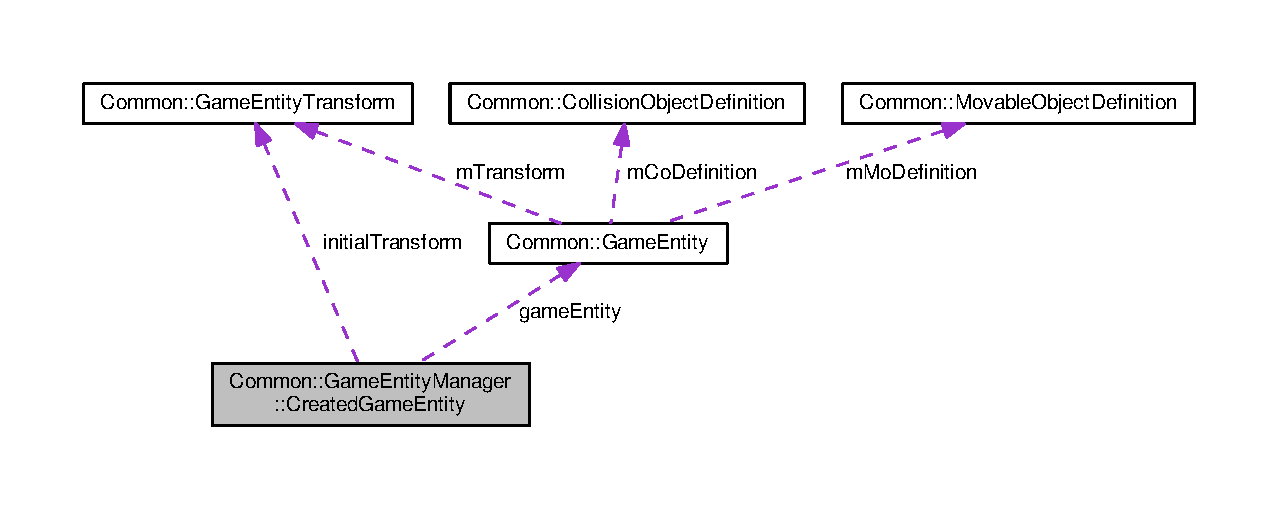
\includegraphics[width=350pt]{struct_common_1_1_game_entity_manager_1_1_created_game_entity__coll__graph}
\end{center}
\end{figure}
\subsection*{Public Attributes}
\begin{DoxyCompactItemize}
\item 
\mbox{\Hypertarget{struct_common_1_1_game_entity_manager_1_1_created_game_entity_aaa44339ada4d32556d43ad60f1620647}\label{struct_common_1_1_game_entity_manager_1_1_created_game_entity_aaa44339ada4d32556d43ad60f1620647}} 
\hyperlink{struct_common_1_1_game_entity}{Game\+Entity} $\ast$ {\bfseries game\+Entity}
\item 
\mbox{\Hypertarget{struct_common_1_1_game_entity_manager_1_1_created_game_entity_a66e0bb365ab3e2396628eb7cc7748eb8}\label{struct_common_1_1_game_entity_manager_1_1_created_game_entity_a66e0bb365ab3e2396628eb7cc7748eb8}} 
\hyperlink{struct_common_1_1_game_entity_transform}{Game\+Entity\+Transform} {\bfseries initial\+Transform}
\end{DoxyCompactItemize}


\subsection{Detailed Description}
Struct describing a \hyperlink{struct_common_1_1_game_entity}{Game\+Entity} and its \hyperlink{struct_common_1_1_game_entity_transform}{Game\+Entity\+Transform}. 

Definition at line 25 of file Game\+Entity\+Manager.\+h.



The documentation for this struct was generated from the following file\+:\begin{DoxyCompactItemize}
\item 
/home/louis/projects/\+Le\+Dernier\+Morkid/\+Common/include/Game\+Entity\+Manager.\+h\end{DoxyCompactItemize}

\hypertarget{struct_common_1_1_game_entity}{}\section{Common\+:\+:Game\+Entity Struct Reference}
\label{struct_common_1_1_game_entity}\index{Common\+::\+Game\+Entity@{Common\+::\+Game\+Entity}}


Struct defining Game Entity.  




{\ttfamily \#include $<$Game\+Entity.\+h$>$}



Collaboration diagram for Common\+:\+:Game\+Entity\+:\nopagebreak
\begin{figure}[H]
\begin{center}
\leavevmode
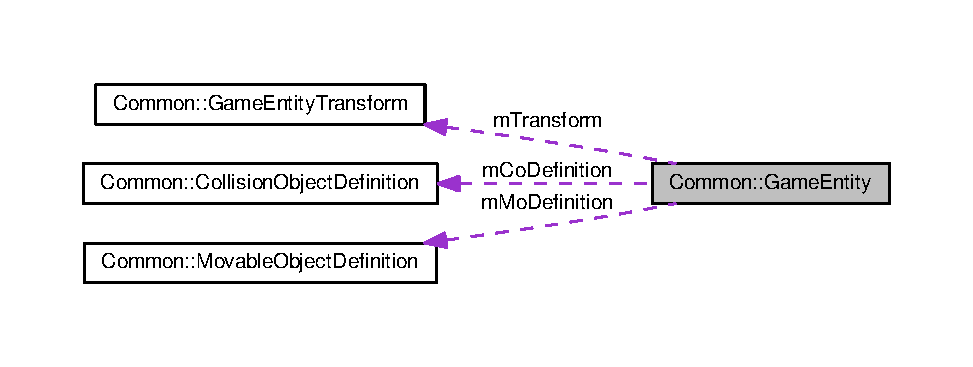
\includegraphics[width=350pt]{struct_common_1_1_game_entity__coll__graph}
\end{center}
\end{figure}
\subsection*{Public Member Functions}
\begin{DoxyCompactItemize}
\item 
\hyperlink{struct_common_1_1_game_entity_a1478181c16b5132fce75352afa88a3a8}{Game\+Entity} (Ogre\+::uint32 id, const \hyperlink{struct_common_1_1_movable_object_definition}{Movable\+Object\+Definition} $\ast$mo\+Definition, const \hyperlink{struct_common_1_1_collision_object_definition}{Collision\+Object\+Definition} $\ast$co\+Definition, Ogre\+::\+Scene\+Memory\+Mgr\+Types type)
\item 
\mbox{\Hypertarget{struct_common_1_1_game_entity_ada4fa423b9c2efaa5ac97f8a081c7d7b}\label{struct_common_1_1_game_entity_ada4fa423b9c2efaa5ac97f8a081c7d7b}} 
Ogre\+::uint32 \hyperlink{struct_common_1_1_game_entity_ada4fa423b9c2efaa5ac97f8a081c7d7b}{get\+Id} (void) const
\begin{DoxyCompactList}\small\item\em Get m\+Id. \end{DoxyCompactList}\item 
bool \hyperlink{struct_common_1_1_game_entity_a9d46d0e1dfa65029ee7acda84b5d648f}{operator$<$} (const \hyperlink{struct_common_1_1_game_entity}{Game\+Entity} $\ast$\+\_\+r) const
\end{DoxyCompactItemize}
\subsection*{Public Attributes}
\begin{DoxyCompactItemize}
\item 
\mbox{\Hypertarget{struct_common_1_1_game_entity_ad6d1c510b4eb3e83e26c2fe78f5ea55c}\label{struct_common_1_1_game_entity_ad6d1c510b4eb3e83e26c2fe78f5ea55c}} 
Ogre\+::\+Scene\+Node $\ast$ \hyperlink{struct_common_1_1_game_entity_ad6d1c510b4eb3e83e26c2fe78f5ea55c}{m\+Scene\+Node}
\begin{DoxyCompactList}\small\item\em Scene\+Node. \end{DoxyCompactList}\item 
\mbox{\Hypertarget{struct_common_1_1_game_entity_aa7394d089e8ddccaeaafd06ced6d2b54}\label{struct_common_1_1_game_entity_aa7394d089e8ddccaeaafd06ced6d2b54}} 
Ogre\+::\+Movable\+Object $\ast$ \hyperlink{struct_common_1_1_game_entity_aa7394d089e8ddccaeaafd06ced6d2b54}{m\+Movable\+Object}
\begin{DoxyCompactList}\small\item\em Movable\+Object. \end{DoxyCompactList}\item 
\mbox{\Hypertarget{struct_common_1_1_game_entity_afa2c88a6b49500a16cba74721a099b84}\label{struct_common_1_1_game_entity_afa2c88a6b49500a16cba74721a099b84}} 
bt\+Collision\+Object $\ast$ \hyperlink{struct_common_1_1_game_entity_afa2c88a6b49500a16cba74721a099b84}{m\+Collision\+Object}
\begin{DoxyCompactList}\small\item\em Collision\+Object. \end{DoxyCompactList}\item 
\mbox{\Hypertarget{struct_common_1_1_game_entity_a36dc8cb7923177eb631dc333e37e22f9}\label{struct_common_1_1_game_entity_a36dc8cb7923177eb631dc333e37e22f9}} 
\hyperlink{struct_common_1_1_game_entity_transform}{Game\+Entity\+Transform} $\ast$ \hyperlink{struct_common_1_1_game_entity_a36dc8cb7923177eb631dc333e37e22f9}{m\+Transform} \mbox{[}N\+U\+M\+\_\+\+G\+A\+M\+E\+\_\+\+E\+N\+T\+I\+T\+Y\+\_\+\+B\+U\+F\+F\+E\+RS\mbox{]}
\begin{DoxyCompactList}\small\item\em Actual transform of the \hyperlink{struct_common_1_1_game_entity}{Game\+Entity}. \end{DoxyCompactList}\item 
\mbox{\Hypertarget{struct_common_1_1_game_entity_a8d91c6cbb06d2c46d2b07b1461b62371}\label{struct_common_1_1_game_entity_a8d91c6cbb06d2c46d2b07b1461b62371}} 
Ogre\+::\+Scene\+Memory\+Mgr\+Types \hyperlink{struct_common_1_1_game_entity_a8d91c6cbb06d2c46d2b07b1461b62371}{m\+Type}
\begin{DoxyCompactList}\small\item\em Type of Scene\+Manager used. \end{DoxyCompactList}\item 
\mbox{\Hypertarget{struct_common_1_1_game_entity_a7e663e00167ef9bf306c474988c949cd}\label{struct_common_1_1_game_entity_a7e663e00167ef9bf306c474988c949cd}} 
\hyperlink{struct_common_1_1_movable_object_definition}{Movable\+Object\+Definition} const  $\ast$ \hyperlink{struct_common_1_1_game_entity_a7e663e00167ef9bf306c474988c949cd}{m\+Mo\+Definition}
\begin{DoxyCompactList}\small\item\em Definition of the Movable\+Object. \end{DoxyCompactList}\item 
\mbox{\Hypertarget{struct_common_1_1_game_entity_a87c7617ad8a3dcdd6dd424cca9fb1079}\label{struct_common_1_1_game_entity_a87c7617ad8a3dcdd6dd424cca9fb1079}} 
\hyperlink{struct_common_1_1_collision_object_definition}{Collision\+Object\+Definition} const  $\ast$ \hyperlink{struct_common_1_1_game_entity_a87c7617ad8a3dcdd6dd424cca9fb1079}{m\+Co\+Definition}
\begin{DoxyCompactList}\small\item\em Definition of the Collision\+Object. \end{DoxyCompactList}\item 
\mbox{\Hypertarget{struct_common_1_1_game_entity_a52127ea487808c64d5e974d2fefcd49b}\label{struct_common_1_1_game_entity_a52127ea487808c64d5e974d2fefcd49b}} 
size\+\_\+t \hyperlink{struct_common_1_1_game_entity_a52127ea487808c64d5e974d2fefcd49b}{m\+Transform\+Buffer\+Idx}
\begin{DoxyCompactList}\small\item\em ID of the transform\textquotesingle{}s buffer. \end{DoxyCompactList}\end{DoxyCompactItemize}
\subsection*{Private Attributes}
\begin{DoxyCompactItemize}
\item 
\mbox{\Hypertarget{struct_common_1_1_game_entity_aade9d274728bf5ed3625fde35d2fd4e7}\label{struct_common_1_1_game_entity_aade9d274728bf5ed3625fde35d2fd4e7}} 
Ogre\+::uint32 \hyperlink{struct_common_1_1_game_entity_aade9d274728bf5ed3625fde35d2fd4e7}{m\+Id}
\begin{DoxyCompactList}\small\item\em Unique ID. \end{DoxyCompactList}\end{DoxyCompactItemize}


\subsection{Detailed Description}
Struct defining Game Entity. 

Definition at line 81 of file Game\+Entity.\+h.



\subsection{Constructor \& Destructor Documentation}
\mbox{\Hypertarget{struct_common_1_1_game_entity_a1478181c16b5132fce75352afa88a3a8}\label{struct_common_1_1_game_entity_a1478181c16b5132fce75352afa88a3a8}} 
\index{Common\+::\+Game\+Entity@{Common\+::\+Game\+Entity}!Game\+Entity@{Game\+Entity}}
\index{Game\+Entity@{Game\+Entity}!Common\+::\+Game\+Entity@{Common\+::\+Game\+Entity}}
\subsubsection{\texorpdfstring{Game\+Entity()}{GameEntity()}}
{\footnotesize\ttfamily Common\+::\+Game\+Entity\+::\+Game\+Entity (\begin{DoxyParamCaption}\item[{Ogre\+::uint32}]{id,  }\item[{const \hyperlink{struct_common_1_1_movable_object_definition}{Movable\+Object\+Definition} $\ast$}]{mo\+Definition,  }\item[{const \hyperlink{struct_common_1_1_collision_object_definition}{Collision\+Object\+Definition} $\ast$}]{co\+Definition,  }\item[{Ogre\+::\+Scene\+Memory\+Mgr\+Types}]{type }\end{DoxyParamCaption})\hspace{0.3cm}{\ttfamily [inline]}}

Constructor 
\begin{DoxyParams}{Parameters}
{\em id} & Unique ID to provide \\
\hline
{\em mo\+Definition} & \hyperlink{struct_common_1_1_movable_object_definition}{Movable\+Object\+Definition} describing Graphics items \\
\hline
{\em co\+Definition} & \hyperlink{struct_common_1_1_collision_object_definition}{Collision\+Object\+Definition} describing Collision item \\
\hline
{\em type} & Type of Scene\+Manager\textquotesingle{}s Memory used (as Ogre\+::\+S\+C\+E\+N\+E\+\_\+\+D\+Y\+N\+A\+M\+IC) \\
\hline
\end{DoxyParams}


Definition at line 130 of file Game\+Entity.\+h.



\subsection{Member Function Documentation}
\mbox{\Hypertarget{struct_common_1_1_game_entity_a9d46d0e1dfa65029ee7acda84b5d648f}\label{struct_common_1_1_game_entity_a9d46d0e1dfa65029ee7acda84b5d648f}} 
\index{Common\+::\+Game\+Entity@{Common\+::\+Game\+Entity}!operator$<$@{operator$<$}}
\index{operator$<$@{operator$<$}!Common\+::\+Game\+Entity@{Common\+::\+Game\+Entity}}
\subsubsection{\texorpdfstring{operator$<$()}{operator<()}}
{\footnotesize\ttfamily bool Common\+::\+Game\+Entity\+::operator$<$ (\begin{DoxyParamCaption}\item[{const \hyperlink{struct_common_1_1_game_entity}{Game\+Entity} $\ast$}]{\+\_\+r }\end{DoxyParamCaption}) const\hspace{0.3cm}{\ttfamily [inline]}}

Compare two \hyperlink{struct_common_1_1_game_entity}{Game\+Entity} 
\begin{DoxyParams}{Parameters}
{\em \+\_\+r} & Second \hyperlink{struct_common_1_1_game_entity}{Game\+Entity} to compare \\
\hline
\end{DoxyParams}
\begin{DoxyReturn}{Returns}
Returns whether \+\_\+r-\/$>$m\+Id is lower than this-\/$>$m\+Id 
\end{DoxyReturn}


Definition at line 154 of file Game\+Entity.\+h.



The documentation for this struct was generated from the following file\+:\begin{DoxyCompactItemize}
\item 
/home/louis/projects/\+Le\+Dernier\+Morkid/\+Common/include/Game\+Entity.\+h\end{DoxyCompactItemize}

\hypertarget{struct_common_1_1_game_entity_cmp}{}\section{Common\+:\+:Game\+Entity\+Cmp Struct Reference}
\label{struct_common_1_1_game_entity_cmp}\index{Common\+::\+Game\+Entity\+Cmp@{Common\+::\+Game\+Entity\+Cmp}}
\subsection*{Public Member Functions}
\begin{DoxyCompactItemize}
\item 
\mbox{\Hypertarget{struct_common_1_1_game_entity_cmp_ab4e0547cba2304e3eefe3e6568df678d}\label{struct_common_1_1_game_entity_cmp_ab4e0547cba2304e3eefe3e6568df678d}} 
bool {\bfseries operator()} (const \hyperlink{struct_common_1_1_game_entity}{Game\+Entity} $\ast$\+\_\+l, const Ogre\+::\+Matrix4 $\ast$R\+E\+S\+T\+R\+I\+C\+T\+\_\+\+A\+L\+I\+AS \+\_\+r) const
\item 
\mbox{\Hypertarget{struct_common_1_1_game_entity_cmp_acc6e1674ddc34ae8992b38c9a2b04e31}\label{struct_common_1_1_game_entity_cmp_acc6e1674ddc34ae8992b38c9a2b04e31}} 
bool {\bfseries operator()} (const Ogre\+::\+Matrix4 $\ast$R\+E\+S\+T\+R\+I\+C\+T\+\_\+\+A\+L\+I\+AS \+\_\+r, const \hyperlink{struct_common_1_1_game_entity}{Game\+Entity} $\ast$\+\_\+l) const
\item 
\mbox{\Hypertarget{struct_common_1_1_game_entity_cmp_adb326666aef6ac6279d3d11eb679ceee}\label{struct_common_1_1_game_entity_cmp_adb326666aef6ac6279d3d11eb679ceee}} 
bool {\bfseries operator()} (const \hyperlink{struct_common_1_1_game_entity}{Game\+Entity} $\ast$\+\_\+l, const \hyperlink{struct_common_1_1_game_entity}{Game\+Entity} $\ast$\+\_\+r) const
\end{DoxyCompactItemize}


\subsection{Detailed Description}


Definition at line 411 of file Graphics\+System.\+cpp.



The documentation for this struct was generated from the following file\+:\begin{DoxyCompactItemize}
\item 
/home/louis/projects/\+Le\+Dernier\+Morkid/\+Common/src/Graphics\+System.\+cpp\end{DoxyCompactItemize}

\hypertarget{class_common_1_1_game_entity_manager}{}\section{Common\+:\+:Game\+Entity\+Manager Class Reference}
\label{class_common_1_1_game_entity_manager}\index{Common\+::\+Game\+Entity\+Manager@{Common\+::\+Game\+Entity\+Manager}}


Class managing \hyperlink{struct_common_1_1_game_entity}{Game\+Entity}.  




{\ttfamily \#include $<$Game\+Entity\+Manager.\+h$>$}



Collaboration diagram for Common\+:\+:Game\+Entity\+Manager\+:\nopagebreak
\begin{figure}[H]
\begin{center}
\leavevmode
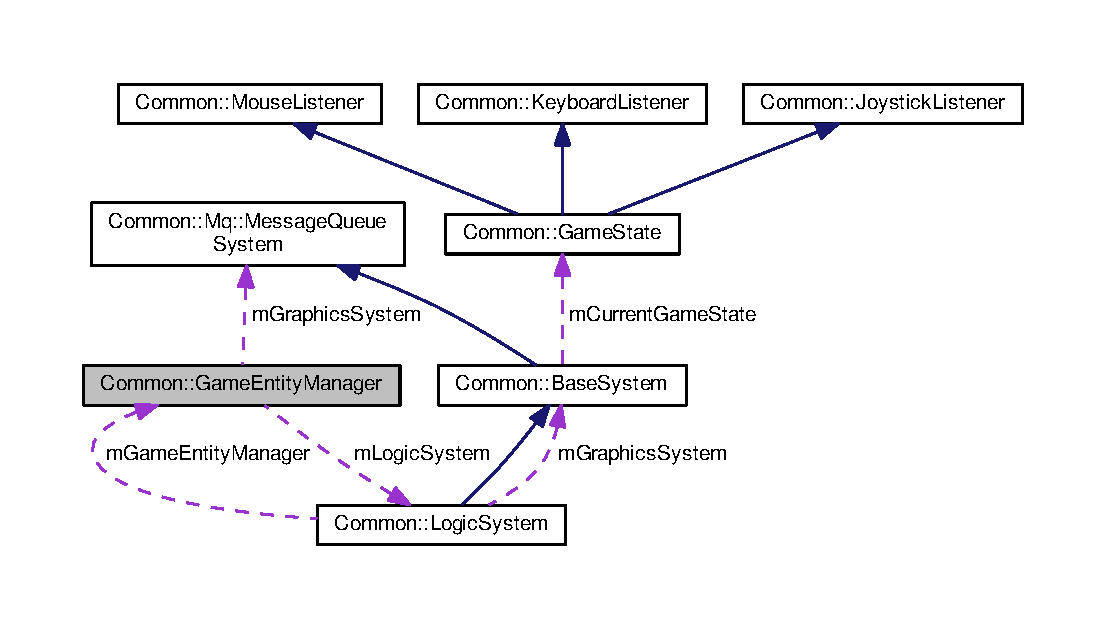
\includegraphics[width=350pt]{class_common_1_1_game_entity_manager__coll__graph}
\end{center}
\end{figure}
\subsection*{Classes}
\begin{DoxyCompactItemize}
\item 
struct \hyperlink{struct_common_1_1_game_entity_manager_1_1_created_game_entity}{Created\+Game\+Entity}
\begin{DoxyCompactList}\small\item\em Struct describing a \hyperlink{struct_common_1_1_game_entity}{Game\+Entity} and its \hyperlink{struct_common_1_1_game_entity_transform}{Game\+Entity\+Transform}. \end{DoxyCompactList}\item 
struct \hyperlink{struct_common_1_1_game_entity_manager_1_1_region}{Region}
\end{DoxyCompactItemize}
\subsection*{Public Types}
\begin{DoxyCompactItemize}
\item 
\mbox{\Hypertarget{class_common_1_1_game_entity_manager_a661304519d61a1bccf8fd1889cb56964}\label{class_common_1_1_game_entity_manager_a661304519d61a1bccf8fd1889cb56964}} 
typedef std\+::vector$<$ Game\+Entity\+Vec $>$ {\bfseries Game\+Entity\+Vec\+Vec}
\end{DoxyCompactItemize}
\subsection*{Public Member Functions}
\begin{DoxyCompactItemize}
\item 
\hyperlink{class_common_1_1_game_entity_manager_abd796010d78cf6d9b6b6f8f7eddbba89}{Game\+Entity\+Manager} (\hyperlink{class_common_1_1_mq_1_1_message_queue_system}{Mq\+::\+Message\+Queue\+System} $\ast$graphics\+System, \hyperlink{class_common_1_1_logic_system}{Logic\+System} $\ast$logic\+System)
\item 
\hyperlink{class_common_1_1_game_entity_manager_aed2c3af1b541c879abf7d78f43085e79}{$\sim$\+Game\+Entity\+Manager} ()
\item 
\hyperlink{struct_common_1_1_game_entity}{Game\+Entity} $\ast$ \hyperlink{class_common_1_1_game_entity_manager_a982abe1d421f8a59fb1ca21ebca97b5f}{add\+Game\+Entity} (Ogre\+::\+Scene\+Memory\+Mgr\+Types type, const \hyperlink{struct_common_1_1_movable_object_definition}{Movable\+Object\+Definition} $\ast$mo\+Definition, const \hyperlink{struct_common_1_1_collision_object_definition}{Collision\+Object\+Definition} $\ast$co\+Definition, const Ogre\+::\+Vector3 \&initial\+Pos, const Ogre\+::\+Quaternion \&initial\+Rot, const Ogre\+::\+Vector3 \&initial\+Scale)
\item 
void \hyperlink{class_common_1_1_game_entity_manager_ab08fbd68fbafbf170abe71f7815b7a13}{remove\+Game\+Entity} (\hyperlink{struct_common_1_1_game_entity}{Game\+Entity} $\ast$to\+Remove)
\item 
void \hyperlink{class_common_1_1_game_entity_manager_ac1cb3aaa00139aaaca96a96e391fa2dc}{\+\_\+notify\+Game\+Entities\+Removed} (size\+\_\+t slot)
\item 
\mbox{\Hypertarget{class_common_1_1_game_entity_manager_a3f8cae1b23e5f53152c1af65b250dcdd}\label{class_common_1_1_game_entity_manager_a3f8cae1b23e5f53152c1af65b250dcdd}} 
void \hyperlink{class_common_1_1_game_entity_manager_a3f8cae1b23e5f53152c1af65b250dcdd}{finish\+Frame\+Parallel} (void)
\begin{DoxyCompactList}\small\item\em Must be called every frame from the L\+O\+G\+IC T\+H\+R\+E\+AD. \end{DoxyCompactList}\end{DoxyCompactItemize}
\subsection*{Private Member Functions}
\begin{DoxyCompactItemize}
\item 
\mbox{\Hypertarget{class_common_1_1_game_entity_manager_a1f5d1d6fa7658fb1b09d38933c3d04d1}\label{class_common_1_1_game_entity_manager_a1f5d1d6fa7658fb1b09d38933c3d04d1}} 
Ogre\+::uint32 {\bfseries get\+Scheduled\+For\+Removal\+Available\+Slot} (void)
\item 
\mbox{\Hypertarget{class_common_1_1_game_entity_manager_a337fbb5e1e9cdd57694c9f87f792ae24}\label{class_common_1_1_game_entity_manager_a337fbb5e1e9cdd57694c9f87f792ae24}} 
void {\bfseries destroy\+All\+Game\+Entities\+In} (Game\+Entity\+Vec \&container)
\item 
\mbox{\Hypertarget{class_common_1_1_game_entity_manager_a6c10977c6e16842aab2e5e230f5039df}\label{class_common_1_1_game_entity_manager_a6c10977c6e16842aab2e5e230f5039df}} 
void {\bfseries aquire\+Transform\+Slot} (size\+\_\+t \&out\+Slot, size\+\_\+t \&out\+Buffer\+Idx)
\item 
\mbox{\Hypertarget{class_common_1_1_game_entity_manager_a409b2f64087e2e8443d6dbe9cd61c928}\label{class_common_1_1_game_entity_manager_a409b2f64087e2e8443d6dbe9cd61c928}} 
void {\bfseries release\+Transform\+Slot} (size\+\_\+t buffer\+Idx, \hyperlink{struct_common_1_1_game_entity_transform}{Game\+Entity\+Transform} $\ast$transform)
\end{DoxyCompactItemize}
\subsection*{Private Attributes}
\begin{DoxyCompactItemize}
\item 
\mbox{\Hypertarget{class_common_1_1_game_entity_manager_a45f10e0964dc22d3db811ff28dc6da55}\label{class_common_1_1_game_entity_manager_a45f10e0964dc22d3db811ff28dc6da55}} 
Ogre\+::uint32 \hyperlink{class_common_1_1_game_entity_manager_a45f10e0964dc22d3db811ff28dc6da55}{m\+Current\+Id}
\begin{DoxyCompactList}\small\item\em Current Id for \hyperlink{struct_common_1_1_game_entity}{Game\+Entity} creating. \end{DoxyCompactList}\item 
\mbox{\Hypertarget{class_common_1_1_game_entity_manager_a7332d715d5c9518860fba2fb0aefc3c9}\label{class_common_1_1_game_entity_manager_a7332d715d5c9518860fba2fb0aefc3c9}} 
Game\+Entity\+Vec \hyperlink{class_common_1_1_game_entity_manager_a7332d715d5c9518860fba2fb0aefc3c9}{m\+Game\+Entities} \mbox{[}Ogre\+::\+N\+U\+M\+\_\+\+S\+C\+E\+N\+E\+\_\+\+M\+E\+M\+O\+R\+Y\+\_\+\+M\+A\+N\+A\+G\+E\+R\+\_\+\+T\+Y\+P\+ES\mbox{]}
\begin{DoxyCompactList}\small\item\em Created \hyperlink{struct_common_1_1_game_entity}{Game\+Entity}. \end{DoxyCompactList}\item 
\mbox{\Hypertarget{class_common_1_1_game_entity_manager_a991cd183485129e72a3144982ea788cf}\label{class_common_1_1_game_entity_manager_a991cd183485129e72a3144982ea788cf}} 
std\+::vector$<$ \hyperlink{struct_common_1_1_game_entity_transform}{Game\+Entity\+Transform} $\ast$ $>$ {\bfseries m\+Transform\+Buffers}
\item 
\mbox{\Hypertarget{class_common_1_1_game_entity_manager_aa068de11d71bc5192d1b92d7d59fbb63}\label{class_common_1_1_game_entity_manager_aa068de11d71bc5192d1b92d7d59fbb63}} 
std\+::vector$<$ \hyperlink{struct_common_1_1_game_entity_manager_1_1_region}{Region} $>$ {\bfseries m\+Available\+Transforms}
\item 
\mbox{\Hypertarget{class_common_1_1_game_entity_manager_a608f0beb843d870520094ba4b46af394}\label{class_common_1_1_game_entity_manager_a608f0beb843d870520094ba4b46af394}} 
Game\+Entity\+Vec\+Vec \hyperlink{class_common_1_1_game_entity_manager_a608f0beb843d870520094ba4b46af394}{m\+Scheduled\+For\+Removal}
\begin{DoxyCompactList}\small\item\em Game\+Entities waiting for removal. \end{DoxyCompactList}\item 
\mbox{\Hypertarget{class_common_1_1_game_entity_manager_a13e1ddfcd9e269ab11836e5f0333dcbb}\label{class_common_1_1_game_entity_manager_a13e1ddfcd9e269ab11836e5f0333dcbb}} 
size\+\_\+t {\bfseries m\+Scheduled\+For\+Removal\+Current\+Slot}
\item 
\mbox{\Hypertarget{class_common_1_1_game_entity_manager_a8e28087a746ac5b44b7c7200226c85f7}\label{class_common_1_1_game_entity_manager_a8e28087a746ac5b44b7c7200226c85f7}} 
std\+::vector$<$ size\+\_\+t $>$ {\bfseries m\+Scheduled\+For\+Removal\+Available\+Slots}
\item 
\mbox{\Hypertarget{class_common_1_1_game_entity_manager_aacead10c62bd45635679ca8161201794}\label{class_common_1_1_game_entity_manager_aacead10c62bd45635679ca8161201794}} 
\hyperlink{class_common_1_1_mq_1_1_message_queue_system}{Mq\+::\+Message\+Queue\+System} $\ast$ \hyperlink{class_common_1_1_game_entity_manager_aacead10c62bd45635679ca8161201794}{m\+Graphics\+System}
\begin{DoxyCompactList}\small\item\em \hyperlink{class_common_1_1_graphics_system}{Graphics\+System} managing Graphics. \end{DoxyCompactList}\item 
\mbox{\Hypertarget{class_common_1_1_game_entity_manager_a9ea718e158804544184545fe7ae5dc6b}\label{class_common_1_1_game_entity_manager_a9ea718e158804544184545fe7ae5dc6b}} 
\hyperlink{class_common_1_1_logic_system}{Logic\+System} $\ast$ \hyperlink{class_common_1_1_game_entity_manager_a9ea718e158804544184545fe7ae5dc6b}{m\+Logic\+System}
\begin{DoxyCompactList}\small\item\em \hyperlink{class_common_1_1_logic_system}{Logic\+System} creating \hyperlink{struct_common_1_1_game_entity}{Game\+Entity}. \end{DoxyCompactList}\end{DoxyCompactItemize}


\subsection{Detailed Description}
Class managing \hyperlink{struct_common_1_1_game_entity}{Game\+Entity}. 

Definition at line 17 of file Game\+Entity\+Manager.\+h.



\subsection{Constructor \& Destructor Documentation}
\mbox{\Hypertarget{class_common_1_1_game_entity_manager_abd796010d78cf6d9b6b6f8f7eddbba89}\label{class_common_1_1_game_entity_manager_abd796010d78cf6d9b6b6f8f7eddbba89}} 
\index{Common\+::\+Game\+Entity\+Manager@{Common\+::\+Game\+Entity\+Manager}!Game\+Entity\+Manager@{Game\+Entity\+Manager}}
\index{Game\+Entity\+Manager@{Game\+Entity\+Manager}!Common\+::\+Game\+Entity\+Manager@{Common\+::\+Game\+Entity\+Manager}}
\subsubsection{\texorpdfstring{Game\+Entity\+Manager()}{GameEntityManager()}}
{\footnotesize\ttfamily Common\+::\+Game\+Entity\+Manager\+::\+Game\+Entity\+Manager (\begin{DoxyParamCaption}\item[{\hyperlink{class_common_1_1_mq_1_1_message_queue_system}{Mq\+::\+Message\+Queue\+System} $\ast$}]{graphics\+System,  }\item[{\hyperlink{class_common_1_1_logic_system}{Logic\+System} $\ast$}]{logic\+System }\end{DoxyParamCaption})}

Constructor 
\begin{DoxyParams}{Parameters}
{\em graphics\+System} & \hyperlink{class_common_1_1_graphics_system}{Graphics\+System} managing Graphics \\
\hline
{\em logic\+System} & \hyperlink{class_common_1_1_logic_system}{Logic\+System} which create the \hyperlink{struct_common_1_1_game_entity}{Game\+Entity} \\
\hline
\end{DoxyParams}


Definition at line 9 of file Game\+Entity\+Manager.\+cpp.

\mbox{\Hypertarget{class_common_1_1_game_entity_manager_aed2c3af1b541c879abf7d78f43085e79}\label{class_common_1_1_game_entity_manager_aed2c3af1b541c879abf7d78f43085e79}} 
\index{Common\+::\+Game\+Entity\+Manager@{Common\+::\+Game\+Entity\+Manager}!````~Game\+Entity\+Manager@{$\sim$\+Game\+Entity\+Manager}}
\index{````~Game\+Entity\+Manager@{$\sim$\+Game\+Entity\+Manager}!Common\+::\+Game\+Entity\+Manager@{Common\+::\+Game\+Entity\+Manager}}
\subsubsection{\texorpdfstring{$\sim$\+Game\+Entity\+Manager()}{~GameEntityManager()}}
{\footnotesize\ttfamily Common\+::\+Game\+Entity\+Manager\+::$\sim$\+Game\+Entity\+Manager (\begin{DoxyParamCaption}{ }\end{DoxyParamCaption})}

Destructor 

Definition at line 18 of file Game\+Entity\+Manager.\+cpp.



\subsection{Member Function Documentation}
\mbox{\Hypertarget{class_common_1_1_game_entity_manager_ac1cb3aaa00139aaaca96a96e391fa2dc}\label{class_common_1_1_game_entity_manager_ac1cb3aaa00139aaaca96a96e391fa2dc}} 
\index{Common\+::\+Game\+Entity\+Manager@{Common\+::\+Game\+Entity\+Manager}!\+\_\+notify\+Game\+Entities\+Removed@{\+\_\+notify\+Game\+Entities\+Removed}}
\index{\+\_\+notify\+Game\+Entities\+Removed@{\+\_\+notify\+Game\+Entities\+Removed}!Common\+::\+Game\+Entity\+Manager@{Common\+::\+Game\+Entity\+Manager}}
\subsubsection{\texorpdfstring{\+\_\+notify\+Game\+Entities\+Removed()}{\_notifyGameEntitiesRemoved()}}
{\footnotesize\ttfamily void Common\+::\+Game\+Entity\+Manager\+::\+\_\+notify\+Game\+Entities\+Removed (\begin{DoxyParamCaption}\item[{size\+\_\+t}]{slot }\end{DoxyParamCaption})}

Notify the Game\+System that a \hyperlink{struct_common_1_1_game_entity}{Game\+Entity} has been removed \begin{DoxyRemark}{Remarks}
Must be called by \hyperlink{class_common_1_1_logic_system}{Logic\+System} when Mq\+::\+G\+A\+M\+E\+\_\+\+E\+N\+T\+I\+T\+Y\+\_\+\+S\+C\+H\+E\+D\+U\+L\+E\+D\+\_\+\+F\+O\+R\+\_\+\+R\+E\+M\+O\+V\+A\+L\+\_\+\+S\+L\+OT message arrives 
\end{DoxyRemark}

\begin{DoxyParams}{Parameters}
{\em Slot} & of the \hyperlink{struct_common_1_1_game_entity}{Game\+Entity} to remove \\
\hline
\end{DoxyParams}


Definition at line 88 of file Game\+Entity\+Manager.\+cpp.

\mbox{\Hypertarget{class_common_1_1_game_entity_manager_a982abe1d421f8a59fb1ca21ebca97b5f}\label{class_common_1_1_game_entity_manager_a982abe1d421f8a59fb1ca21ebca97b5f}} 
\index{Common\+::\+Game\+Entity\+Manager@{Common\+::\+Game\+Entity\+Manager}!add\+Game\+Entity@{add\+Game\+Entity}}
\index{add\+Game\+Entity@{add\+Game\+Entity}!Common\+::\+Game\+Entity\+Manager@{Common\+::\+Game\+Entity\+Manager}}
\subsubsection{\texorpdfstring{add\+Game\+Entity()}{addGameEntity()}}
{\footnotesize\ttfamily \hyperlink{struct_common_1_1_game_entity}{Game\+Entity} $\ast$ Common\+::\+Game\+Entity\+Manager\+::add\+Game\+Entity (\begin{DoxyParamCaption}\item[{Ogre\+::\+Scene\+Memory\+Mgr\+Types}]{type,  }\item[{const \hyperlink{struct_common_1_1_movable_object_definition}{Movable\+Object\+Definition} $\ast$}]{mo\+Definition,  }\item[{const \hyperlink{struct_common_1_1_collision_object_definition}{Collision\+Object\+Definition} $\ast$}]{co\+Definition,  }\item[{const Ogre\+::\+Vector3 \&}]{initial\+Pos,  }\item[{const Ogre\+::\+Quaternion \&}]{initial\+Rot,  }\item[{const Ogre\+::\+Vector3 \&}]{initial\+Scale }\end{DoxyParamCaption})}

Creates a \hyperlink{struct_common_1_1_game_entity}{Game\+Entity}, adding it to the world, and scheduling for the Graphics thread to create the appropiate Scene\+Node and Item pointers. M\+U\+ST BE C\+A\+L\+L\+ED F\+R\+OM L\+O\+G\+IC T\+H\+R\+E\+AD. 
\begin{DoxyParams}{Parameters}
{\em type} & Whether this \hyperlink{struct_common_1_1_game_entity}{Game\+Entity} is dynamic (going to change transform frequently), or static (will move/rotate/scale very, very infrequently) \\
\hline
{\em mo\+Definition} & Definition of the Movable\+Object (Graphics) \\
\hline
{\em co\+Definition} & Definition of the Collision\+Object (Collisions) \\
\hline
{\em initial\+Pos} & Starting position of the \hyperlink{struct_common_1_1_game_entity}{Game\+Entity} \\
\hline
{\em initial\+Rot} & Starting orientation of the \hyperlink{struct_common_1_1_game_entity}{Game\+Entity} \\
\hline
{\em initial\+Scale} & Starting scale of the \hyperlink{struct_common_1_1_game_entity}{Game\+Entity} \\
\hline
\end{DoxyParams}
\begin{DoxyReturn}{Returns}
Pointer of \hyperlink{struct_common_1_1_game_entity}{Game\+Entity} ready to be used by the Logic thread. Take in mind not all of its pointers may filled yet (the ones that are not meant to be used by the logic thread) 
\end{DoxyReturn}


Definition at line 44 of file Game\+Entity\+Manager.\+cpp.

\mbox{\Hypertarget{class_common_1_1_game_entity_manager_ab08fbd68fbafbf170abe71f7815b7a13}\label{class_common_1_1_game_entity_manager_ab08fbd68fbafbf170abe71f7815b7a13}} 
\index{Common\+::\+Game\+Entity\+Manager@{Common\+::\+Game\+Entity\+Manager}!remove\+Game\+Entity@{remove\+Game\+Entity}}
\index{remove\+Game\+Entity@{remove\+Game\+Entity}!Common\+::\+Game\+Entity\+Manager@{Common\+::\+Game\+Entity\+Manager}}
\subsubsection{\texorpdfstring{remove\+Game\+Entity()}{removeGameEntity()}}
{\footnotesize\ttfamily void Common\+::\+Game\+Entity\+Manager\+::remove\+Game\+Entity (\begin{DoxyParamCaption}\item[{\hyperlink{struct_common_1_1_game_entity}{Game\+Entity} $\ast$}]{to\+Remove }\end{DoxyParamCaption})}

Removes the \hyperlink{struct_common_1_1_game_entity}{Game\+Entity} from the world. The pointer is not immediately destroyed, we first need to release data in other threads (i.\+e. Graphics). It will be destroyed after the Render thread confirms it is done with it (via a Mq\+::\+G\+A\+M\+E\+\_\+\+E\+N\+T\+I\+T\+Y\+\_\+\+S\+C\+H\+E\+D\+U\+L\+E\+D\+\_\+\+F\+O\+R\+\_\+\+R\+E\+M\+O\+V\+A\+L\+\_\+\+S\+L\+OT message) 
\begin{DoxyParams}{Parameters}
{\em to\+Remove} & \hyperlink{struct_common_1_1_game_entity}{Game\+Entity} to remove \\
\hline
\end{DoxyParams}


Definition at line 77 of file Game\+Entity\+Manager.\+cpp.



The documentation for this class was generated from the following files\+:\begin{DoxyCompactItemize}
\item 
/home/louis/projects/\+Le\+Dernier\+Morkid/\+Common/include/Game\+Entity\+Manager.\+h\item 
/home/louis/projects/\+Le\+Dernier\+Morkid/\+Common/src/Game\+Entity\+Manager.\+cpp\end{DoxyCompactItemize}

\hypertarget{struct_common_1_1_game_entity_transform}{}\section{Common\+:\+:Game\+Entity\+Transform Struct Reference}
\label{struct_common_1_1_game_entity_transform}\index{Common\+::\+Game\+Entity\+Transform@{Common\+::\+Game\+Entity\+Transform}}
\subsection*{Public Attributes}
\begin{DoxyCompactItemize}
\item 
\mbox{\Hypertarget{struct_common_1_1_game_entity_transform_adb2f2de17915c25bb9d4c67d44fe0fd1}\label{struct_common_1_1_game_entity_transform_adb2f2de17915c25bb9d4c67d44fe0fd1}} 
Ogre\+::\+Vector3 {\bfseries v\+Pos}
\item 
\mbox{\Hypertarget{struct_common_1_1_game_entity_transform_acd1fccda4d680b79073f5a6d7bb198d4}\label{struct_common_1_1_game_entity_transform_acd1fccda4d680b79073f5a6d7bb198d4}} 
Ogre\+::\+Quaternion {\bfseries q\+Rot}
\item 
\mbox{\Hypertarget{struct_common_1_1_game_entity_transform_a47cc10b536e85e01efe0cd86185c4c0d}\label{struct_common_1_1_game_entity_transform_a47cc10b536e85e01efe0cd86185c4c0d}} 
Ogre\+::\+Vector3 {\bfseries v\+Scale}
\end{DoxyCompactItemize}


The documentation for this struct was generated from the following file\+:\begin{DoxyCompactItemize}
\item 
/home/louis/projects/\+Le\+Dernier\+Morkid/\+Common/include/Game\+Entity.\+h\end{DoxyCompactItemize}

\hypertarget{class_common_1_1_game_state}{}\section{Common\+:\+:Game\+State Class Reference}
\label{class_common_1_1_game_state}\index{Common\+::\+Game\+State@{Common\+::\+Game\+State}}


Inheritance diagram for Common\+:\+:Game\+State\+:\nopagebreak
\begin{figure}[H]
\begin{center}
\leavevmode
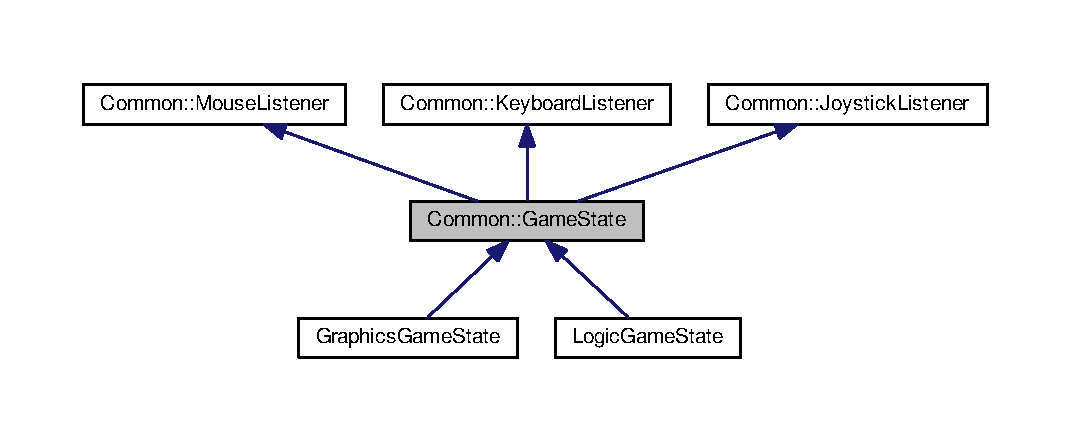
\includegraphics[width=350pt]{class_common_1_1_game_state__inherit__graph}
\end{center}
\end{figure}


Collaboration diagram for Common\+:\+:Game\+State\+:\nopagebreak
\begin{figure}[H]
\begin{center}
\leavevmode
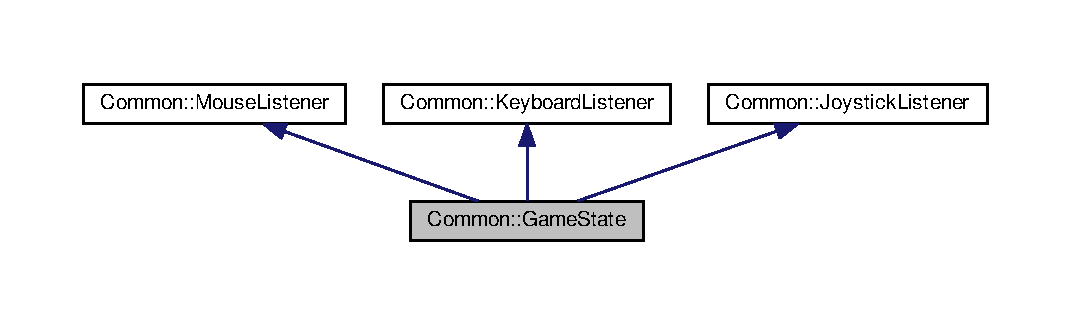
\includegraphics[width=350pt]{class_common_1_1_game_state__coll__graph}
\end{center}
\end{figure}
\subsection*{Public Member Functions}
\begin{DoxyCompactItemize}
\item 
\mbox{\Hypertarget{class_common_1_1_game_state_a4e7fa2fbc9080111213ce379eb33d082}\label{class_common_1_1_game_state_a4e7fa2fbc9080111213ce379eb33d082}} 
virtual void {\bfseries initialize} (void)
\item 
\mbox{\Hypertarget{class_common_1_1_game_state_a7cda78fa6c4a405ead90c6e0bc895c85}\label{class_common_1_1_game_state_a7cda78fa6c4a405ead90c6e0bc895c85}} 
virtual void {\bfseries deinitialize} (void)
\item 
\mbox{\Hypertarget{class_common_1_1_game_state_a30b77d03dd849ebb2d6698686e9e7619}\label{class_common_1_1_game_state_a30b77d03dd849ebb2d6698686e9e7619}} 
virtual void {\bfseries create\+Scene} (void)
\item 
\mbox{\Hypertarget{class_common_1_1_game_state_a03176055b9cb064b2cea5b64cbf6647a}\label{class_common_1_1_game_state_a03176055b9cb064b2cea5b64cbf6647a}} 
virtual void {\bfseries destroy\+Scene} (void)
\item 
\mbox{\Hypertarget{class_common_1_1_game_state_a38271924996d8c1bbdcbfee6ffe63f95}\label{class_common_1_1_game_state_a38271924996d8c1bbdcbfee6ffe63f95}} 
virtual void {\bfseries update} (float time\+Since\+Last)
\item 
\mbox{\Hypertarget{class_common_1_1_game_state_af9d8b5d245f12f68432653a50de46ca4}\label{class_common_1_1_game_state_af9d8b5d245f12f68432653a50de46ca4}} 
virtual void {\bfseries finish\+Frame\+Parallel} (void)
\item 
\mbox{\Hypertarget{class_common_1_1_game_state_ade96417c05bf3ad03e5bea4ee8578d89}\label{class_common_1_1_game_state_ade96417c05bf3ad03e5bea4ee8578d89}} 
virtual void {\bfseries finish\+Frame} (void)
\end{DoxyCompactItemize}


The documentation for this class was generated from the following file\+:\begin{DoxyCompactItemize}
\item 
/home/louis/projects/\+Le\+Dernier\+Morkid/\+Common/include/Game\+State.\+h\end{DoxyCompactItemize}

\hypertarget{class_graphics_game_state}{}\section{Graphics\+Game\+State Class Reference}
\label{class_graphics_game_state}\index{Graphics\+Game\+State@{Graphics\+Game\+State}}


Inheritance diagram for Graphics\+Game\+State\+:\nopagebreak
\begin{figure}[H]
\begin{center}
\leavevmode
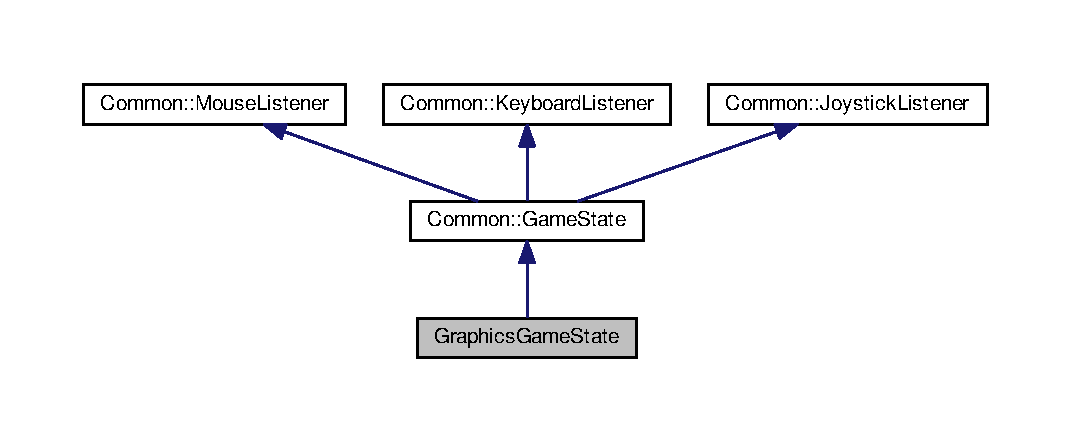
\includegraphics[width=350pt]{class_graphics_game_state__inherit__graph}
\end{center}
\end{figure}


Collaboration diagram for Graphics\+Game\+State\+:\nopagebreak
\begin{figure}[H]
\begin{center}
\leavevmode
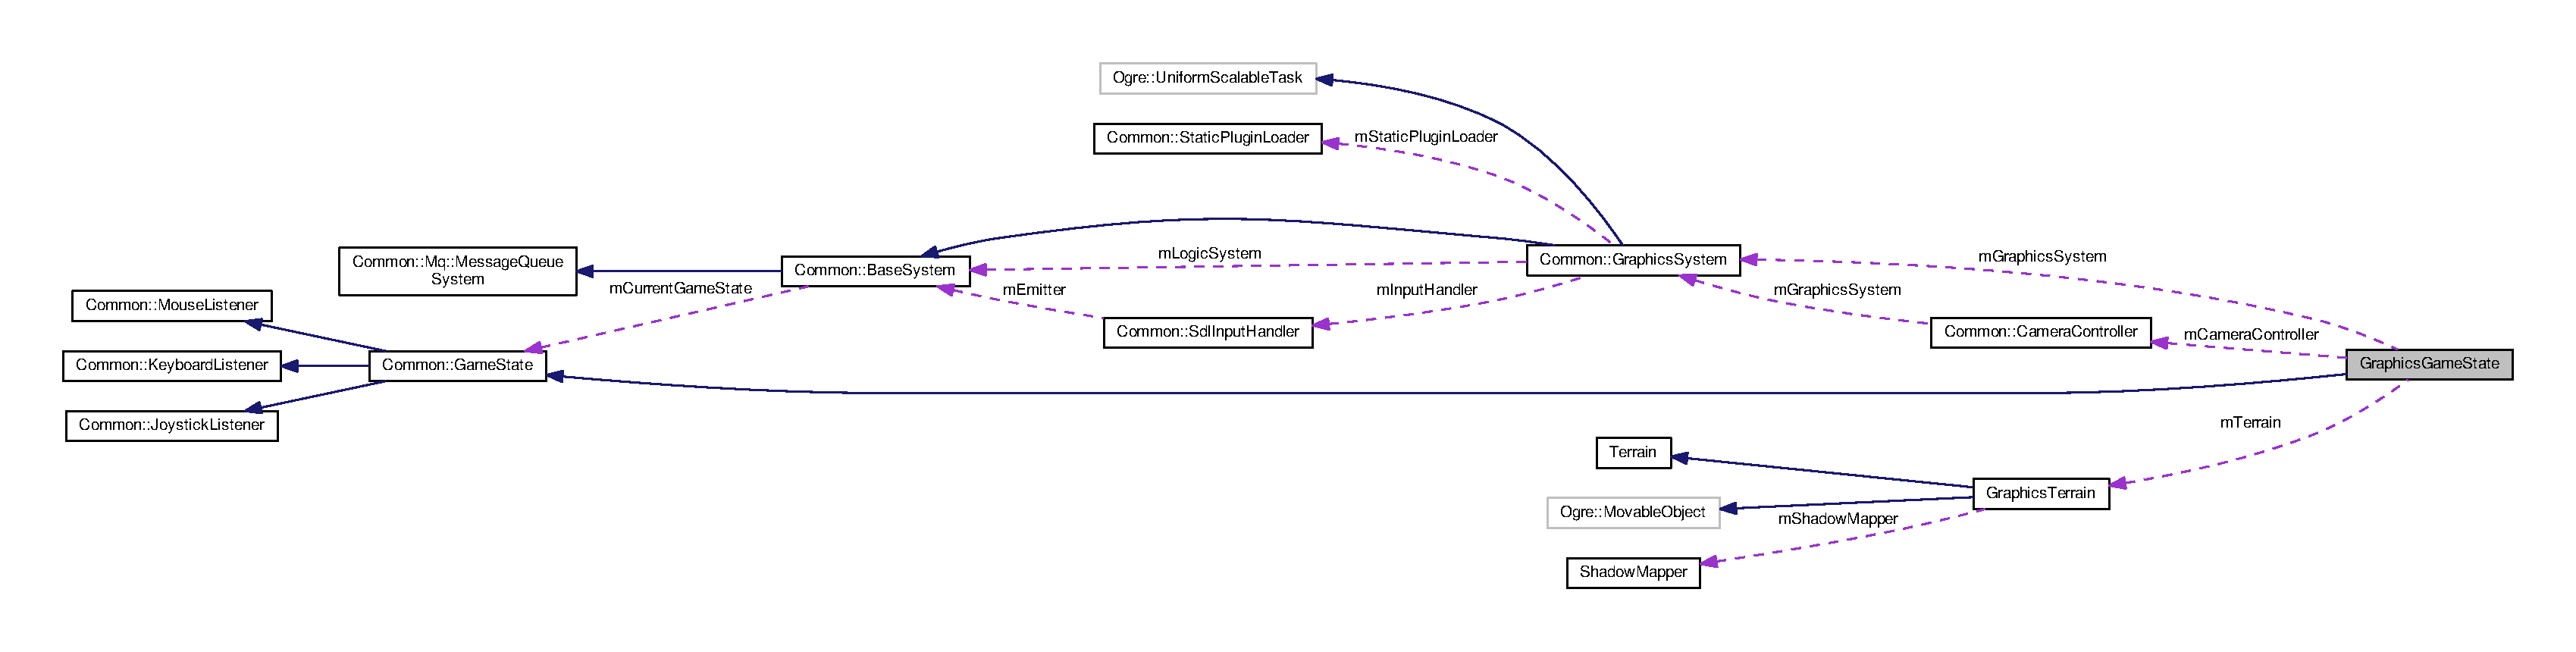
\includegraphics[width=350pt]{class_graphics_game_state__coll__graph}
\end{center}
\end{figure}
\subsection*{Public Member Functions}
\begin{DoxyCompactItemize}
\item 
\mbox{\Hypertarget{class_graphics_game_state_a0e81886306b906569add56b43e8da91d}\label{class_graphics_game_state_a0e81886306b906569add56b43e8da91d}} 
void {\bfseries \+\_\+notify\+Graphics\+System} (\hyperlink{class_common_1_1_graphics_system}{Common\+::\+Graphics\+System} $\ast$graphics\+System)
\item 
\mbox{\Hypertarget{class_graphics_game_state_af8e2cd857387dd301edc894bfb8a7ac5}\label{class_graphics_game_state_af8e2cd857387dd301edc894bfb8a7ac5}} 
virtual void \hyperlink{class_graphics_game_state_af8e2cd857387dd301edc894bfb8a7ac5}{create\+Scene} (void)
\begin{DoxyCompactList}\small\item\em Create the scene. \end{DoxyCompactList}\item 
virtual void \hyperlink{class_graphics_game_state_a5a2543a4cdd551c98f4540707bc7213e}{update} (float time\+Since\+Last)
\item 
\mbox{\Hypertarget{class_graphics_game_state_ae7a7e707169e5c0cdbe2f54c8b1be2f6}\label{class_graphics_game_state_ae7a7e707169e5c0cdbe2f54c8b1be2f6}} 
virtual void \hyperlink{class_graphics_game_state_ae7a7e707169e5c0cdbe2f54c8b1be2f6}{key\+Pressed} (const \hyperlink{struct_s_d_l___keyboard_event}{S\+D\+L\+\_\+\+Keyboard\+Event} \&arg)
\begin{DoxyCompactList}\small\item\em Function called when a key is pressed. \end{DoxyCompactList}\item 
\mbox{\Hypertarget{class_graphics_game_state_a9a63e8acad9cb3d9e3c389f88e303665}\label{class_graphics_game_state_a9a63e8acad9cb3d9e3c389f88e303665}} 
virtual void \hyperlink{class_graphics_game_state_a9a63e8acad9cb3d9e3c389f88e303665}{key\+Released} (const \hyperlink{struct_s_d_l___keyboard_event}{S\+D\+L\+\_\+\+Keyboard\+Event} \&arg)
\begin{DoxyCompactList}\small\item\em Function called when a key is released. \end{DoxyCompactList}\item 
\mbox{\Hypertarget{class_graphics_game_state_acdf08d6cfd2610be0186047adbda912e}\label{class_graphics_game_state_acdf08d6cfd2610be0186047adbda912e}} 
virtual void \hyperlink{class_graphics_game_state_acdf08d6cfd2610be0186047adbda912e}{mouse\+Moved} (const \hyperlink{union_s_d_l___event}{S\+D\+L\+\_\+\+Event} \&arg)
\begin{DoxyCompactList}\small\item\em Function called when mouse is moved. \end{DoxyCompactList}\end{DoxyCompactItemize}
\subsection*{Protected Member Functions}
\begin{DoxyCompactItemize}
\item 
\mbox{\Hypertarget{class_graphics_game_state_a5cb40a6795b789595dbdec2c28f420b8}\label{class_graphics_game_state_a5cb40a6795b789595dbdec2c28f420b8}} 
Ogre\+::\+Compositor\+Workspace $\ast$ {\bfseries setup\+Compositor} ()
\end{DoxyCompactItemize}
\subsection*{Protected Attributes}
\begin{DoxyCompactItemize}
\item 
\mbox{\Hypertarget{class_graphics_game_state_ad6d8656a6af5861d756f8e677a06567d}\label{class_graphics_game_state_ad6d8656a6af5861d756f8e677a06567d}} 
bool {\bfseries m\+Enable\+Interpolation}
\item 
\mbox{\Hypertarget{class_graphics_game_state_a6931ab79c90541e4e3cc93cd79a733f6}\label{class_graphics_game_state_a6931ab79c90541e4e3cc93cd79a733f6}} 
\hyperlink{class_common_1_1_graphics_system}{Common\+::\+Graphics\+System} $\ast$ {\bfseries m\+Graphics\+System}
\item 
\mbox{\Hypertarget{class_graphics_game_state_a2debaa701782161be4b2376872a9194c}\label{class_graphics_game_state_a2debaa701782161be4b2376872a9194c}} 
\hyperlink{class_common_1_1_camera_controller}{Common\+::\+Camera\+Controller} $\ast$ {\bfseries m\+Camera\+Controller}
\item 
\mbox{\Hypertarget{class_graphics_game_state_a9f260815846c0fc225ff59a2dda90b27}\label{class_graphics_game_state_a9f260815846c0fc225ff59a2dda90b27}} 
\hyperlink{class_graphics_terrain}{Graphics\+Terrain} $\ast$ {\bfseries m\+Terrain}
\item 
\mbox{\Hypertarget{class_graphics_game_state_a59e90f7396f9ae5db563c3be4ac89139}\label{class_graphics_game_state_a59e90f7396f9ae5db563c3be4ac89139}} 
Ogre\+::\+Light $\ast$ {\bfseries m\+Sun\+Light}
\end{DoxyCompactItemize}


\subsection{Detailed Description}


Definition at line 14 of file Graphics\+Game\+State.\+h.



\subsection{Member Function Documentation}
\mbox{\Hypertarget{class_graphics_game_state_a5a2543a4cdd551c98f4540707bc7213e}\label{class_graphics_game_state_a5a2543a4cdd551c98f4540707bc7213e}} 
\index{Graphics\+Game\+State@{Graphics\+Game\+State}!update@{update}}
\index{update@{update}!Graphics\+Game\+State@{Graphics\+Game\+State}}
\subsubsection{\texorpdfstring{update()}{update()}}
{\footnotesize\ttfamily void Graphics\+Game\+State\+::update (\begin{DoxyParamCaption}\item[{float}]{time\+Since\+Last }\end{DoxyParamCaption})\hspace{0.3cm}{\ttfamily [virtual]}}

Update the Game\+State param time\+Since\+Last Time past since last frame 

Reimplemented from \hyperlink{class_common_1_1_game_state_a38271924996d8c1bbdcbfee6ffe63f95}{Common\+::\+Game\+State}.



Definition at line 135 of file Graphics\+Game\+State.\+cpp.



The documentation for this class was generated from the following files\+:\begin{DoxyCompactItemize}
\item 
/home/louis/projects/\+Le\+Dernier\+Morkid/include/\+Graphics/Graphics\+Game\+State.\+h\item 
/home/louis/projects/\+Le\+Dernier\+Morkid/src/\+Graphics/Graphics\+Game\+State.\+cpp\end{DoxyCompactItemize}

\hypertarget{class_common_1_1_graphics_system}{}\section{Common\+:\+:Graphics\+System Class Reference}
\label{class_common_1_1_graphics_system}\index{Common\+::\+Graphics\+System@{Common\+::\+Graphics\+System}}


Inheritance diagram for Common\+:\+:Graphics\+System\+:\nopagebreak
\begin{figure}[H]
\begin{center}
\leavevmode
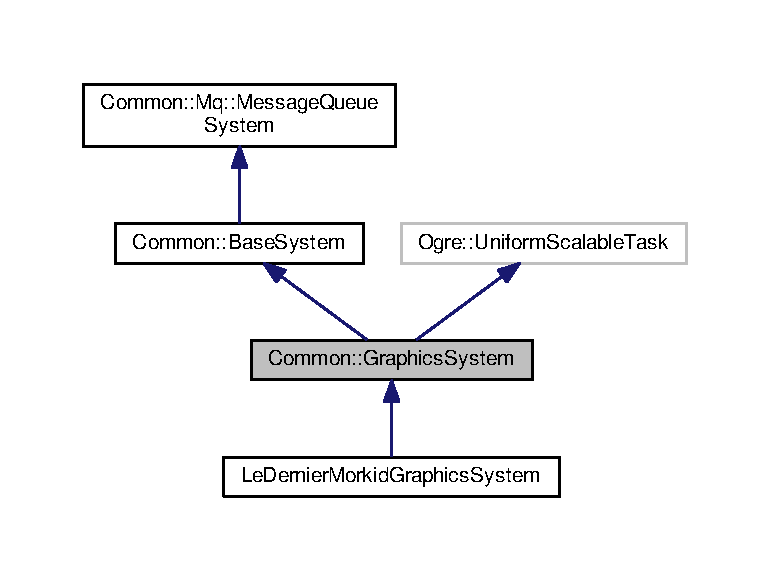
\includegraphics[width=350pt]{class_common_1_1_graphics_system__inherit__graph}
\end{center}
\end{figure}


Collaboration diagram for Common\+:\+:Graphics\+System\+:\nopagebreak
\begin{figure}[H]
\begin{center}
\leavevmode
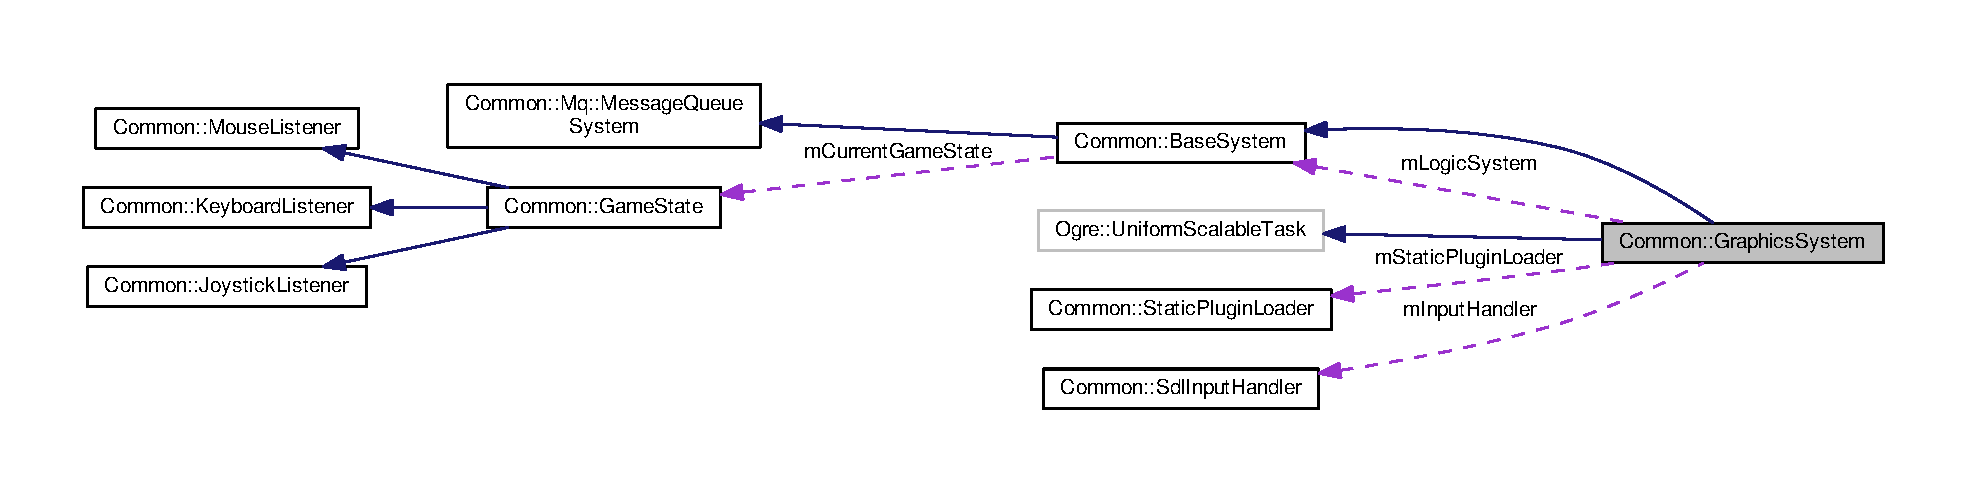
\includegraphics[width=350pt]{class_common_1_1_graphics_system__coll__graph}
\end{center}
\end{figure}
\subsection*{Public Member Functions}
\begin{DoxyCompactItemize}
\item 
\mbox{\Hypertarget{class_common_1_1_graphics_system_a640e8520e276805c15f12d340a7b6090}\label{class_common_1_1_graphics_system_a640e8520e276805c15f12d340a7b6090}} 
{\bfseries Graphics\+System} (\hyperlink{class_common_1_1_game_state}{Game\+State} $\ast$game\+State, Ogre\+::\+Colour\+Value background\+Colour=Ogre\+::\+Colour\+Value(0.f, 0.f, 0.f))
\item 
\mbox{\Hypertarget{class_common_1_1_graphics_system_a1bbb04c3ab640d4753f852d17a419df0}\label{class_common_1_1_graphics_system_a1bbb04c3ab640d4753f852d17a419df0}} 
void {\bfseries \+\_\+notify\+Logic\+System} (\hyperlink{class_common_1_1_base_system}{Base\+System} $\ast$logic\+System)
\item 
\mbox{\Hypertarget{class_common_1_1_graphics_system_ad6aec10b001fbfc10cd86cd009615745}\label{class_common_1_1_graphics_system_ad6aec10b001fbfc10cd86cd009615745}} 
void {\bfseries initialize} (const Ogre\+::\+String \&window\+Title)
\item 
\mbox{\Hypertarget{class_common_1_1_graphics_system_ade2d4efd6e535d312818a92230eb7dcf}\label{class_common_1_1_graphics_system_ade2d4efd6e535d312818a92230eb7dcf}} 
void {\bfseries deinitialize} (void)
\item 
\mbox{\Hypertarget{class_common_1_1_graphics_system_ab2c01af1a20132c37964f34f7dfb645c}\label{class_common_1_1_graphics_system_ab2c01af1a20132c37964f34f7dfb645c}} 
void {\bfseries update} (float time\+Since\+Last)
\item 
\mbox{\Hypertarget{class_common_1_1_graphics_system_a9cabbf2ae25610cfa006d45a95f77d6a}\label{class_common_1_1_graphics_system_a9cabbf2ae25610cfa006d45a95f77d6a}} 
void {\bfseries update\+Game\+Entities} (const Game\+Entity\+Vec \&game\+Entities, float weight)
\item 
\mbox{\Hypertarget{class_common_1_1_graphics_system_af262817d8290de7fe06e88e424bd5588}\label{class_common_1_1_graphics_system_af262817d8290de7fe06e88e424bd5588}} 
virtual void {\bfseries execute} (size\+\_\+t thread\+Id, size\+\_\+t num\+Threads)
\item 
\mbox{\Hypertarget{class_common_1_1_graphics_system_af658d1a3d1037affc4bce8a63ea33514}\label{class_common_1_1_graphics_system_af658d1a3d1037affc4bce8a63ea33514}} 
const Game\+Entity\+Vec \& {\bfseries get\+Game\+Entities} (Ogre\+::\+Scene\+Memory\+Mgr\+Types type) const
\item 
\mbox{\Hypertarget{class_common_1_1_graphics_system_a3996ebbb7e250c04cbf107efafd34984}\label{class_common_1_1_graphics_system_a3996ebbb7e250c04cbf107efafd34984}} 
\hyperlink{class_common_1_1_sdl_input_handler}{Sdl\+Input\+Handler} $\ast$ {\bfseries get\+Input\+Handler} (void)
\item 
\mbox{\Hypertarget{class_common_1_1_graphics_system_acdbed0670eef23789a3c68e00d88ac4c}\label{class_common_1_1_graphics_system_acdbed0670eef23789a3c68e00d88ac4c}} 
void {\bfseries set\+Quit} (void)
\item 
\mbox{\Hypertarget{class_common_1_1_graphics_system_a216f755133f87e2074a36a556d303e41}\label{class_common_1_1_graphics_system_a216f755133f87e2074a36a556d303e41}} 
bool {\bfseries get\+Quit} (void) const
\item 
\mbox{\Hypertarget{class_common_1_1_graphics_system_a4a9abd5c431c9e61b48d4d167f775935}\label{class_common_1_1_graphics_system_a4a9abd5c431c9e61b48d4d167f775935}} 
float {\bfseries get\+Accum\+Time\+Since\+Last\+Logic\+Frame} (void) const
\item 
\mbox{\Hypertarget{class_common_1_1_graphics_system_a0890b804419adb1857d359810dec34ff}\label{class_common_1_1_graphics_system_a0890b804419adb1857d359810dec34ff}} 
Ogre\+::\+Root $\ast$ {\bfseries get\+Root} (void) const
\item 
\mbox{\Hypertarget{class_common_1_1_graphics_system_a7b330688e6c66c74e23ec57eab54f341}\label{class_common_1_1_graphics_system_a7b330688e6c66c74e23ec57eab54f341}} 
Ogre\+::\+Render\+Window $\ast$ {\bfseries get\+Render\+Window} (void) const
\item 
\mbox{\Hypertarget{class_common_1_1_graphics_system_aef392cd73eb9571778a0910e9b991cac}\label{class_common_1_1_graphics_system_aef392cd73eb9571778a0910e9b991cac}} 
Ogre\+::\+Scene\+Manager $\ast$ {\bfseries get\+Scene\+Manager} (void) const
\item 
\mbox{\Hypertarget{class_common_1_1_graphics_system_a7497c78b142d7dd1461418a75804bc58}\label{class_common_1_1_graphics_system_a7497c78b142d7dd1461418a75804bc58}} 
Ogre\+::\+Camera $\ast$ {\bfseries get\+Camera} (void) const
\item 
\mbox{\Hypertarget{class_common_1_1_graphics_system_a24280225a9fd08efd4ac9100c7de07c0}\label{class_common_1_1_graphics_system_a24280225a9fd08efd4ac9100c7de07c0}} 
Ogre\+::\+Compositor\+Workspace $\ast$ {\bfseries get\+Compositor\+Workspace} (void) const
\item 
\mbox{\Hypertarget{class_common_1_1_graphics_system_aab69bdc895c97c506caab1fa828b575a}\label{class_common_1_1_graphics_system_aab69bdc895c97c506caab1fa828b575a}} 
virtual void {\bfseries stop\+Compositor} (void)
\item 
\mbox{\Hypertarget{class_common_1_1_graphics_system_aa7a5a6ce9e1da97940f5af5785bb4a8a}\label{class_common_1_1_graphics_system_aa7a5a6ce9e1da97940f5af5785bb4a8a}} 
virtual void {\bfseries restart\+Compositor} (void)
\end{DoxyCompactItemize}
\subsection*{Public Attributes}
\begin{DoxyCompactItemize}
\item 
\mbox{\Hypertarget{class_common_1_1_graphics_system_a0fd3f9ba43027f8dcebeda885302e564}\label{class_common_1_1_graphics_system_a0fd3f9ba43027f8dcebeda885302e564}} 
\hyperlink{class_common_1_1_base_system}{Base\+System} $\ast$ {\bfseries m\+Logic\+System}
\end{DoxyCompactItemize}
\subsection*{Protected Member Functions}
\begin{DoxyCompactItemize}
\item 
\mbox{\Hypertarget{class_common_1_1_graphics_system_a16f86321da0331beaa393b9e1bbd48bd}\label{class_common_1_1_graphics_system_a16f86321da0331beaa393b9e1bbd48bd}} 
void {\bfseries handle\+Window\+Event} (const \hyperlink{union_s_d_l___event}{S\+D\+L\+\_\+\+Event} \&evt)
\item 
\mbox{\Hypertarget{class_common_1_1_graphics_system_a8d286a151ed9a65f0eebe1ac119e2d59}\label{class_common_1_1_graphics_system_a8d286a151ed9a65f0eebe1ac119e2d59}} 
virtual void {\bfseries process\+Incoming\+Message} (Mq\+::\+Message\+Id message\+Id, const void $\ast$data)
\item 
\mbox{\Hypertarget{class_common_1_1_graphics_system_a6ca699c2cd358f6101d7c00f605a515a}\label{class_common_1_1_graphics_system_a6ca699c2cd358f6101d7c00f605a515a}} 
virtual void {\bfseries setup\+Resources} (void)
\item 
\mbox{\Hypertarget{class_common_1_1_graphics_system_a17ad5ae3ca1efd63f7436d977e7f2657}\label{class_common_1_1_graphics_system_a17ad5ae3ca1efd63f7436d977e7f2657}} 
virtual void {\bfseries register\+Hlms} (void)
\item 
\mbox{\Hypertarget{class_common_1_1_graphics_system_ab91bf390248b3098db3b739e066092b1}\label{class_common_1_1_graphics_system_ab91bf390248b3098db3b739e066092b1}} 
virtual void {\bfseries load\+Resources} (void)
\item 
\mbox{\Hypertarget{class_common_1_1_graphics_system_a6fc846f42d2011cfdeb465aa9ef44b20}\label{class_common_1_1_graphics_system_a6fc846f42d2011cfdeb465aa9ef44b20}} 
virtual void {\bfseries choose\+Scene\+Manager} (void)
\item 
\mbox{\Hypertarget{class_common_1_1_graphics_system_a84373ea7cef6f794831d98ef60227abb}\label{class_common_1_1_graphics_system_a84373ea7cef6f794831d98ef60227abb}} 
virtual void {\bfseries create\+Camera} (void)
\item 
\mbox{\Hypertarget{class_common_1_1_graphics_system_a36c3548e669676eb5ad328d947454e81}\label{class_common_1_1_graphics_system_a36c3548e669676eb5ad328d947454e81}} 
virtual Ogre\+::\+Compositor\+Workspace $\ast$ {\bfseries setup\+Compositor} (void)
\item 
\mbox{\Hypertarget{class_common_1_1_graphics_system_a0c9ba8a9470920fe8dd3d19ad85698e0}\label{class_common_1_1_graphics_system_a0c9ba8a9470920fe8dd3d19ad85698e0}} 
virtual void {\bfseries create\+Resource\+Listener} (void)
\item 
\mbox{\Hypertarget{class_common_1_1_graphics_system_aaaac50f8c51dad1746ef48aaf87cad8d}\label{class_common_1_1_graphics_system_aaaac50f8c51dad1746ef48aaf87cad8d}} 
void {\bfseries game\+Entity\+Added} (const \hyperlink{struct_common_1_1_game_entity_manager_1_1_created_game_entity}{Game\+Entity\+Manager\+::\+Created\+Game\+Entity} $\ast$created\+Game\+Entity)
\item 
\mbox{\Hypertarget{class_common_1_1_graphics_system_ad10ea4363b7d49f6a43bee937b031559}\label{class_common_1_1_graphics_system_ad10ea4363b7d49f6a43bee937b031559}} 
void {\bfseries game\+Entity\+Removed} (\hyperlink{struct_common_1_1_game_entity}{Game\+Entity} $\ast$to\+Remove)
\end{DoxyCompactItemize}
\subsection*{Static Protected Member Functions}
\begin{DoxyCompactItemize}
\item 
\mbox{\Hypertarget{class_common_1_1_graphics_system_a25c1257066ca90c4c6d9cf0dc1fa2bfb}\label{class_common_1_1_graphics_system_a25c1257066ca90c4c6d9cf0dc1fa2bfb}} 
static void {\bfseries add\+Resource\+Location} (const Ogre\+::\+String \&arch\+Name, const Ogre\+::\+String \&type\+Name, const Ogre\+::\+String \&sec\+Name)
\end{DoxyCompactItemize}
\subsection*{Protected Attributes}
\begin{DoxyCompactItemize}
\item 
\mbox{\Hypertarget{class_common_1_1_graphics_system_a92bb62174a5eb357a6765c31891649b5}\label{class_common_1_1_graphics_system_a92bb62174a5eb357a6765c31891649b5}} 
S\+D\+L\+\_\+\+Window $\ast$ {\bfseries m\+Sdl\+Window}
\item 
\mbox{\Hypertarget{class_common_1_1_graphics_system_a9ddbb67b87143d1c124e55a96d875150}\label{class_common_1_1_graphics_system_a9ddbb67b87143d1c124e55a96d875150}} 
\hyperlink{class_common_1_1_sdl_input_handler}{Sdl\+Input\+Handler} $\ast$ {\bfseries m\+Input\+Handler}
\item 
\mbox{\Hypertarget{class_common_1_1_graphics_system_adf9abc6e0d78256c7b8d2b16c01a6b98}\label{class_common_1_1_graphics_system_adf9abc6e0d78256c7b8d2b16c01a6b98}} 
Ogre\+::\+Root $\ast$ {\bfseries m\+Root}
\item 
\mbox{\Hypertarget{class_common_1_1_graphics_system_a14a142b2ccd792b6b50b9240b8b03bcd}\label{class_common_1_1_graphics_system_a14a142b2ccd792b6b50b9240b8b03bcd}} 
Ogre\+::\+Render\+Window $\ast$ {\bfseries m\+Render\+Window}
\item 
\mbox{\Hypertarget{class_common_1_1_graphics_system_a6510b0288e263ca79514eccbc80e52d2}\label{class_common_1_1_graphics_system_a6510b0288e263ca79514eccbc80e52d2}} 
Ogre\+::\+Scene\+Manager $\ast$ {\bfseries m\+Scene\+Manager}
\item 
\mbox{\Hypertarget{class_common_1_1_graphics_system_ac8f3870f3218f13e7883262d9db2ba0d}\label{class_common_1_1_graphics_system_ac8f3870f3218f13e7883262d9db2ba0d}} 
Ogre\+::\+Camera $\ast$ {\bfseries m\+Camera}
\item 
\mbox{\Hypertarget{class_common_1_1_graphics_system_a5a80c19583bedfc79a0366d0d94be657}\label{class_common_1_1_graphics_system_a5a80c19583bedfc79a0366d0d94be657}} 
Ogre\+::\+Compositor\+Workspace $\ast$ {\bfseries m\+Workspace}
\item 
\mbox{\Hypertarget{class_common_1_1_graphics_system_ad9d14ea53f9f8ddfd3025c58665c469c}\label{class_common_1_1_graphics_system_ad9d14ea53f9f8ddfd3025c58665c469c}} 
Ogre\+::\+String {\bfseries m\+Plugins\+Path}
\item 
\mbox{\Hypertarget{class_common_1_1_graphics_system_acf0f1cb58173eca575b63dbea1010415}\label{class_common_1_1_graphics_system_acf0f1cb58173eca575b63dbea1010415}} 
Ogre\+::\+String {\bfseries m\+Write\+Access\+Folder}
\item 
\mbox{\Hypertarget{class_common_1_1_graphics_system_ad6c40d2244340da36c0a7853dc891196}\label{class_common_1_1_graphics_system_ad6c40d2244340da36c0a7853dc891196}} 
Ogre\+::\+String {\bfseries m\+Resource\+Path}
\item 
\mbox{\Hypertarget{class_common_1_1_graphics_system_a94edce8cb6c70b67a66ea65a4c989fce}\label{class_common_1_1_graphics_system_a94edce8cb6c70b67a66ea65a4c989fce}} 
\hyperlink{class_common_1_1_static_plugin_loader}{Static\+Plugin\+Loader} {\bfseries m\+Static\+Plugin\+Loader}
\item 
\mbox{\Hypertarget{class_common_1_1_graphics_system_ad8f0298ee17a2331e0e6406e16e6cd23}\label{class_common_1_1_graphics_system_ad8f0298ee17a2331e0e6406e16e6cd23}} 
float {\bfseries m\+Accum\+Time\+Since\+Last\+Logic\+Frame}
\item 
\mbox{\Hypertarget{class_common_1_1_graphics_system_a2a3acd30c5c38530b9b07f0b3a2dbce5}\label{class_common_1_1_graphics_system_a2a3acd30c5c38530b9b07f0b3a2dbce5}} 
Ogre\+::uint32 {\bfseries m\+Current\+Transform\+Idx}
\item 
\mbox{\Hypertarget{class_common_1_1_graphics_system_a39c347647fabbfb8d86a8e7fc55825bd}\label{class_common_1_1_graphics_system_a39c347647fabbfb8d86a8e7fc55825bd}} 
Game\+Entity\+Vec {\bfseries m\+Game\+Entities} \mbox{[}Ogre\+::\+N\+U\+M\+\_\+\+S\+C\+E\+N\+E\+\_\+\+M\+E\+M\+O\+R\+Y\+\_\+\+M\+A\+N\+A\+G\+E\+R\+\_\+\+T\+Y\+P\+ES\mbox{]}
\item 
\mbox{\Hypertarget{class_common_1_1_graphics_system_adaf0d898cd16130084bdf36220f6111b}\label{class_common_1_1_graphics_system_adaf0d898cd16130084bdf36220f6111b}} 
Game\+Entity\+Vec const  $\ast$ {\bfseries m\+Thread\+Game\+Entity\+To\+Update}
\item 
\mbox{\Hypertarget{class_common_1_1_graphics_system_a41e916be28a4d889337a4c8c0868b3ed}\label{class_common_1_1_graphics_system_a41e916be28a4d889337a4c8c0868b3ed}} 
float {\bfseries m\+Thread\+Weight}
\item 
\mbox{\Hypertarget{class_common_1_1_graphics_system_a141239a20891b1a980e319a89420f2b0}\label{class_common_1_1_graphics_system_a141239a20891b1a980e319a89420f2b0}} 
bool {\bfseries m\+Quit}
\item 
\mbox{\Hypertarget{class_common_1_1_graphics_system_a64e431c0b8b4a8913e488a845afdc48d}\label{class_common_1_1_graphics_system_a64e431c0b8b4a8913e488a845afdc48d}} 
Ogre\+::\+Colour\+Value {\bfseries m\+Background\+Colour}
\end{DoxyCompactItemize}


The documentation for this class was generated from the following files\+:\begin{DoxyCompactItemize}
\item 
/home/louis/projects/\+Le\+Dernier\+Morkid/\+Common/include/Graphics\+System.\+h\item 
/home/louis/projects/\+Le\+Dernier\+Morkid/\+Common/src/Graphics\+System.\+cpp\end{DoxyCompactItemize}

\hypertarget{class_graphics_terrain}{}\section{Graphics\+Terrain Class Reference}
\label{class_graphics_terrain}\index{Graphics\+Terrain@{Graphics\+Terrain}}


Inheritance diagram for Graphics\+Terrain\+:\nopagebreak
\begin{figure}[H]
\begin{center}
\leavevmode
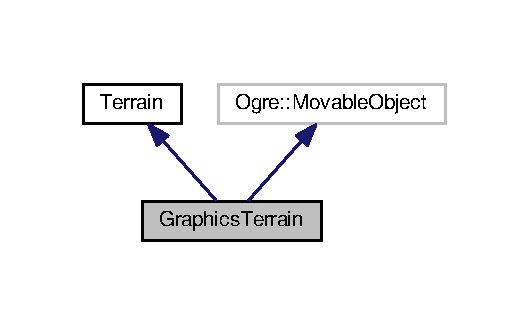
\includegraphics[width=254pt]{class_graphics_terrain__inherit__graph}
\end{center}
\end{figure}


Collaboration diagram for Graphics\+Terrain\+:\nopagebreak
\begin{figure}[H]
\begin{center}
\leavevmode
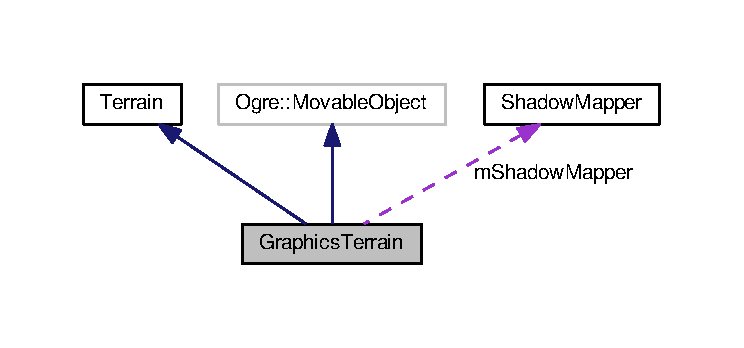
\includegraphics[width=350pt]{class_graphics_terrain__coll__graph}
\end{center}
\end{figure}
\subsection*{Public Member Functions}
\begin{DoxyCompactItemize}
\item 
\mbox{\Hypertarget{class_graphics_terrain_ad09f3393bcb3dc279e0f682ec836532c}\label{class_graphics_terrain_ad09f3393bcb3dc279e0f682ec836532c}} 
{\bfseries Graphics\+Terrain} (Ogre\+::\+Id\+Type id, Ogre\+::\+Object\+Memory\+Manager $\ast$object\+Memory\+Manager, Ogre\+::\+Scene\+Manager $\ast$scene\+Manager, Ogre\+::uint8 render\+Queue\+Id, Ogre\+::\+Compositor\+Manager2 $\ast$compositor\+Manager, Ogre\+::\+Camera $\ast$camera)
\item 
\mbox{\Hypertarget{class_graphics_terrain_ab8dbd55a773ceb3940ac85e0d79eaced}\label{class_graphics_terrain_ab8dbd55a773ceb3940ac85e0d79eaced}} 
void {\bfseries load} (const Ogre\+::\+String \&tex\+Name, const Ogre\+::\+Vector3 center, const Ogre\+::\+Vector3 \&dimensions)
\item 
\mbox{\Hypertarget{class_graphics_terrain_ad97766d268fc7fd379bf40f4194739d4}\label{class_graphics_terrain_ad97766d268fc7fd379bf40f4194739d4}} 
void {\bfseries update} (const Ogre\+::\+Vector3 \&light\+Dir, float light\+Epsilon=1e-\/6f)
\item 
\mbox{\Hypertarget{class_graphics_terrain_a437b37d2a5cc809b26d73e10856e73e9}\label{class_graphics_terrain_a437b37d2a5cc809b26d73e10856e73e9}} 
const \hyperlink{class_shadow_mapper}{Shadow\+Mapper} $\ast$ {\bfseries get\+Shadow\+Mapper} (void) const
\item 
\mbox{\Hypertarget{class_graphics_terrain_aed6da11b79b85601fe23059fb4eaeb56}\label{class_graphics_terrain_aed6da11b79b85601fe23059fb4eaeb56}} 
const Ogre\+::\+String \& {\bfseries get\+Movable\+Type} (void) const
\item 
\mbox{\Hypertarget{class_graphics_terrain_a30e288df42390fb9df74d3bf8ed5575f}\label{class_graphics_terrain_a30e288df42390fb9df74d3bf8ed5575f}} 
Ogre\+::\+Texture\+Ptr {\bfseries get\+Height\+Map\+Tex} (void) const
\item 
\mbox{\Hypertarget{class_graphics_terrain_a8cfec476235c065efb3d7d29168a8495}\label{class_graphics_terrain_a8cfec476235c065efb3d7d29168a8495}} 
Ogre\+::\+Texture\+Ptr {\bfseries get\+Normal\+Map\+Tex} (void) const
\item 
\mbox{\Hypertarget{class_graphics_terrain_ad52653eed5c22be28e7a185f0eed87b7}\label{class_graphics_terrain_ad52653eed5c22be28e7a185f0eed87b7}} 
Ogre\+::\+Texture\+Ptr {\bfseries \+\_\+get\+Shadow\+Map\+Tex} (void) const
\item 
\mbox{\Hypertarget{class_graphics_terrain_af5b0244ad8598ede54145e5398726e26}\label{class_graphics_terrain_af5b0244ad8598ede54145e5398726e26}} 
void {\bfseries set\+Datablock} (Ogre\+::\+Hlms\+Datablock $\ast$datablock)
\end{DoxyCompactItemize}
\subsection*{Protected Member Functions}
\begin{DoxyCompactItemize}
\item 
\mbox{\Hypertarget{class_graphics_terrain_a18e6c99d2b81a64230a0d8aab48ed6f4}\label{class_graphics_terrain_a18e6c99d2b81a64230a0d8aab48ed6f4}} 
void {\bfseries create\+Normal\+Texture} (void)
\item 
\mbox{\Hypertarget{class_graphics_terrain_a93d81648750634ca5e420f671f0277d3}\label{class_graphics_terrain_a93d81648750634ca5e420f671f0277d3}} 
void {\bfseries destroy\+Normal\+Texture} (void)
\item 
\mbox{\Hypertarget{class_graphics_terrain_a492e06b03ef8462322469d961e192b46}\label{class_graphics_terrain_a492e06b03ef8462322469d961e192b46}} 
void {\bfseries add\+Renderable} (const \hyperlink{struct_grid_point}{Grid\+Point} \&grid\+Pos, const \hyperlink{struct_grid_point}{Grid\+Point} \&cell\+Size, Ogre\+::uint32 lod\+Level)
\item 
\mbox{\Hypertarget{class_graphics_terrain_a35615fa429a0eeda2b5ea8fe908bbc5a}\label{class_graphics_terrain_a35615fa429a0eeda2b5ea8fe908bbc5a}} 
void {\bfseries optimize\+Cells\+And\+Add} (void)
\item 
\mbox{\Hypertarget{class_graphics_terrain_a4633b2fde146e8acde31db85fba26832}\label{class_graphics_terrain_a4633b2fde146e8acde31db85fba26832}} 
bool {\bfseries is\+Visible} (const \hyperlink{struct_grid_point}{Grid\+Point} \&g\+Pos, const \hyperlink{struct_grid_point}{Grid\+Point} \&g\+Size) const
\end{DoxyCompactItemize}
\subsection*{Protected Attributes}
\begin{DoxyCompactItemize}
\item 
\mbox{\Hypertarget{class_graphics_terrain_a7c44ecd3372c8fc18414b45e48cd08b4}\label{class_graphics_terrain_a7c44ecd3372c8fc18414b45e48cd08b4}} 
std\+::vector$<$ \hyperlink{class_terrain_cell}{Terrain\+Cell} $>$ {\bfseries m\+Terrain\+Cells}
\item 
\mbox{\Hypertarget{class_graphics_terrain_a99431a62bb984a130be408d8e198f74e}\label{class_graphics_terrain_a99431a62bb984a130be408d8e198f74e}} 
std\+::vector$<$ \hyperlink{class_terrain_cell}{Terrain\+Cell} $\ast$ $>$ {\bfseries m\+Collected\+Cells} \mbox{[}2\mbox{]}
\item 
\mbox{\Hypertarget{class_graphics_terrain_a88383b43425ca55d6fbb5ef1e20302a3}\label{class_graphics_terrain_a88383b43425ca55d6fbb5ef1e20302a3}} 
size\+\_\+t {\bfseries m\+Current\+Cell}
\item 
\mbox{\Hypertarget{class_graphics_terrain_a7f43e03a4fe4c0811648b299397dc4da}\label{class_graphics_terrain_a7f43e03a4fe4c0811648b299397dc4da}} 
Ogre\+::\+Texture\+Ptr {\bfseries m\+Normal\+Map\+Tex}
\item 
\mbox{\Hypertarget{class_graphics_terrain_aea152cbc9b9a33faed38e5fad97aa793}\label{class_graphics_terrain_aea152cbc9b9a33faed38e5fad97aa793}} 
Ogre\+::\+Vector3 {\bfseries m\+Prev\+Light\+Dir}
\item 
\mbox{\Hypertarget{class_graphics_terrain_aeb60344dfe412f9241348c96fa29f9ec}\label{class_graphics_terrain_aeb60344dfe412f9241348c96fa29f9ec}} 
\hyperlink{class_shadow_mapper}{Shadow\+Mapper} $\ast$ {\bfseries m\+Shadow\+Mapper}
\item 
\mbox{\Hypertarget{class_graphics_terrain_a80d73f6cdce5b43211188f6bda9fc633}\label{class_graphics_terrain_a80d73f6cdce5b43211188f6bda9fc633}} 
Ogre\+::\+Compositor\+Manager2 $\ast$ {\bfseries m\+Compositor\+Manager}
\item 
\mbox{\Hypertarget{class_graphics_terrain_afd48f23d6b969ccef286bb1aec437340}\label{class_graphics_terrain_afd48f23d6b969ccef286bb1aec437340}} 
Ogre\+::\+Camera $\ast$ {\bfseries m\+Camera}
\end{DoxyCompactItemize}


The documentation for this class was generated from the following files\+:\begin{DoxyCompactItemize}
\item 
/home/louis/projects/\+Le\+Dernier\+Morkid/include/\+Terrain/Graphics\+Terrain.\+h\item 
/home/louis/projects/\+Le\+Dernier\+Morkid/src/\+Terrain/Graphics\+Terrain.\+cpp\end{DoxyCompactItemize}

\hypertarget{struct_grid_direction}{}\section{Grid\+Direction Struct Reference}
\label{struct_grid_direction}\index{Grid\+Direction@{Grid\+Direction}}
\subsection*{Public Attributes}
\begin{DoxyCompactItemize}
\item 
\mbox{\Hypertarget{struct_grid_direction_a290ac1961ef3d29c634d482c235f86de}\label{struct_grid_direction_a290ac1961ef3d29c634d482c235f86de}} 
int {\bfseries x}
\item 
\mbox{\Hypertarget{struct_grid_direction_afb0df84ade3f8e9b6b0adec5b7294c32}\label{struct_grid_direction_afb0df84ade3f8e9b6b0adec5b7294c32}} 
int {\bfseries z}
\end{DoxyCompactItemize}


The documentation for this struct was generated from the following file\+:\begin{DoxyCompactItemize}
\item 
/home/louis/projects/\+Le\+Dernier\+Morkid/include/\+Terrain/Terrain.\+h\end{DoxyCompactItemize}

\hypertarget{struct_grid_point}{}\section{Grid\+Point Struct Reference}
\label{struct_grid_point}\index{Grid\+Point@{Grid\+Point}}
\subsection*{Public Attributes}
\begin{DoxyCompactItemize}
\item 
\mbox{\Hypertarget{struct_grid_point_a6a2d6291fb359df17bdcce483c8283ee}\label{struct_grid_point_a6a2d6291fb359df17bdcce483c8283ee}} 
Ogre\+::int32 {\bfseries x}
\item 
\mbox{\Hypertarget{struct_grid_point_a99f578ff1addf4e0ecd9c425f271a915}\label{struct_grid_point_a99f578ff1addf4e0ecd9c425f271a915}} 
Ogre\+::int32 {\bfseries z}
\end{DoxyCompactItemize}


\subsection{Detailed Description}


Definition at line 10 of file Terrain.\+h.



The documentation for this struct was generated from the following file\+:\begin{DoxyCompactItemize}
\item 
/home/louis/projects/\+Le\+Dernier\+Morkid/include/\+Terrain/Terrain.\+h\end{DoxyCompactItemize}

\hypertarget{class_hlms_pbs_terrain_shadows}{}\section{Hlms\+Pbs\+Terrain\+Shadows Class Reference}
\label{class_hlms_pbs_terrain_shadows}\index{Hlms\+Pbs\+Terrain\+Shadows@{Hlms\+Pbs\+Terrain\+Shadows}}


Inheritance diagram for Hlms\+Pbs\+Terrain\+Shadows\+:\nopagebreak
\begin{figure}[H]
\begin{center}
\leavevmode
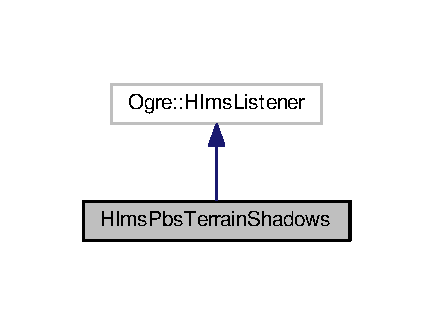
\includegraphics[width=208pt]{class_hlms_pbs_terrain_shadows__inherit__graph}
\end{center}
\end{figure}


Collaboration diagram for Hlms\+Pbs\+Terrain\+Shadows\+:\nopagebreak
\begin{figure}[H]
\begin{center}
\leavevmode
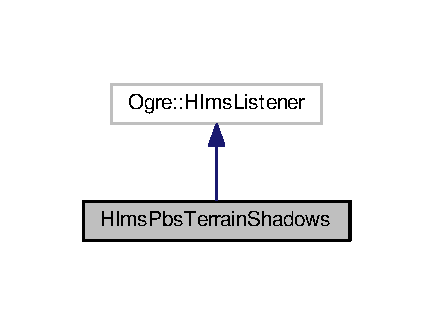
\includegraphics[width=208pt]{class_hlms_pbs_terrain_shadows__coll__graph}
\end{center}
\end{figure}
\subsection*{Public Member Functions}
\begin{DoxyCompactItemize}
\item 
\mbox{\Hypertarget{class_hlms_pbs_terrain_shadows_abc0156c34287dc229fc6bcd5dd926042}\label{class_hlms_pbs_terrain_shadows_abc0156c34287dc229fc6bcd5dd926042}} 
void {\bfseries set\+Terrain} (\hyperlink{class_graphics_terrain}{Graphics\+Terrain} $\ast$terra)
\item 
\mbox{\Hypertarget{class_hlms_pbs_terrain_shadows_a5d6c59561dd58544669c41271f96673b}\label{class_hlms_pbs_terrain_shadows_a5d6c59561dd58544669c41271f96673b}} 
virtual void {\bfseries shader\+Cache\+Entry\+Created} (const Ogre\+::\+String \&shader\+Profile, const Ogre\+::\+Hlms\+Cache $\ast$hlms\+Cache\+Entry, const Ogre\+::\+Hlms\+Cache \&pass\+Cache, const Ogre\+::\+Hlms\+Property\+Vec \&properties, const Ogre\+::\+Queued\+Renderable \&queued\+Renderable)
\item 
\mbox{\Hypertarget{class_hlms_pbs_terrain_shadows_ad8aab96d71ac61b3774d6b454455cf5c}\label{class_hlms_pbs_terrain_shadows_ad8aab96d71ac61b3774d6b454455cf5c}} 
virtual void {\bfseries prepare\+Pass\+Hash} (const Ogre\+::\+Compositor\+Shadow\+Node $\ast$shadow\+Node, bool caster\+Pass, bool dual\+Paraboloid, Ogre\+::\+Scene\+Manager $\ast$scene\+Manager, Ogre\+::\+Hlms $\ast$hlms)
\item 
\mbox{\Hypertarget{class_hlms_pbs_terrain_shadows_a71a669419504ad94fd31213ae547224f}\label{class_hlms_pbs_terrain_shadows_a71a669419504ad94fd31213ae547224f}} 
virtual Ogre\+::uint32 {\bfseries get\+Pass\+Buffer\+Size} (const Ogre\+::\+Compositor\+Shadow\+Node $\ast$shadow\+Node, bool caster\+Pass, bool dual\+Paraboloid, Ogre\+::\+Scene\+Manager $\ast$scene\+Manager) const
\item 
\mbox{\Hypertarget{class_hlms_pbs_terrain_shadows_ad963e7633a906fd8b8ad4963a08f4770}\label{class_hlms_pbs_terrain_shadows_ad963e7633a906fd8b8ad4963a08f4770}} 
virtual float $\ast$ {\bfseries prepare\+Pass\+Buffer} (const Ogre\+::\+Compositor\+Shadow\+Node $\ast$shadow\+Node, bool caster\+Pass, bool dual\+Paraboloid, Ogre\+::\+Scene\+Manager $\ast$scene\+Manager, float $\ast$pass\+Buffer\+Ptr)
\item 
\mbox{\Hypertarget{class_hlms_pbs_terrain_shadows_aac00263a92c1b2ba60e10b87896f99cd}\label{class_hlms_pbs_terrain_shadows_aac00263a92c1b2ba60e10b87896f99cd}} 
virtual void {\bfseries hlms\+Type\+Changed} (bool caster\+Pass, Ogre\+::\+Command\+Buffer $\ast$command\+Buffer, const Ogre\+::\+Hlms\+Datablock $\ast$datablock)
\end{DoxyCompactItemize}


The documentation for this class was generated from the following files\+:\begin{DoxyCompactItemize}
\item 
/home/louis/projects/\+Le\+Dernier\+Morkid/include/\+Terrain/\+Hlms/\+Pbs\+Listener/Hlms\+Pbs\+Terrain\+Shadows.\+h\item 
/home/louis/projects/\+Le\+Dernier\+Morkid/src/\+Terrain/\+Hlms/\+Pbs\+Listener/Hlms\+Pbs\+Terrain\+Shadows.\+cpp\end{DoxyCompactItemize}

\hypertarget{class_hlms_terrain}{}\section{Hlms\+Terrain Class Reference}
\label{class_hlms_terrain}\index{Hlms\+Terrain@{Hlms\+Terrain}}


{\ttfamily \#include $<$Hlms\+Terrain.\+h$>$}



Inheritance diagram for Hlms\+Terrain\+:\nopagebreak
\begin{figure}[H]
\begin{center}
\leavevmode
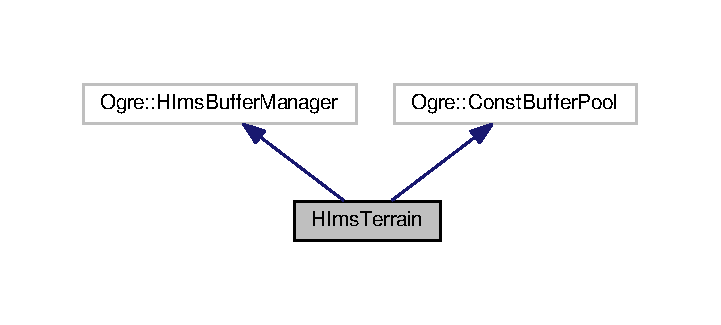
\includegraphics[width=346pt]{class_hlms_terrain__inherit__graph}
\end{center}
\end{figure}


Collaboration diagram for Hlms\+Terrain\+:\nopagebreak
\begin{figure}[H]
\begin{center}
\leavevmode
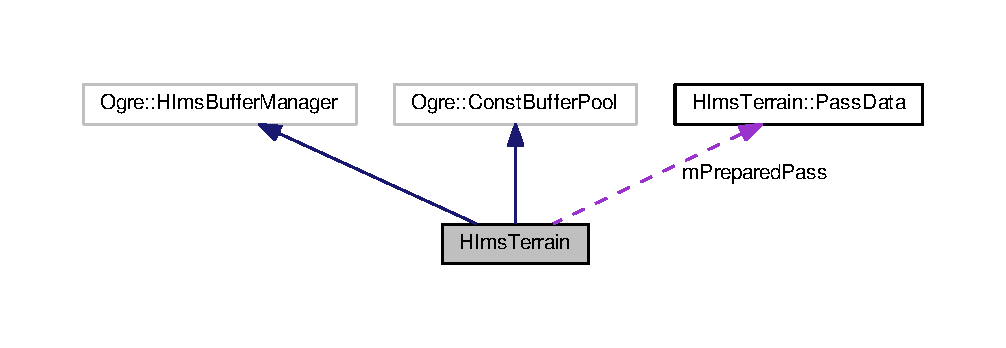
\includegraphics[width=350pt]{class_hlms_terrain__coll__graph}
\end{center}
\end{figure}
\subsection*{Classes}
\begin{DoxyCompactItemize}
\item 
struct \hyperlink{struct_hlms_terrain_1_1_pass_data}{Pass\+Data}
\end{DoxyCompactItemize}
\subsection*{Public Types}
\begin{DoxyCompactItemize}
\item 
enum \hyperlink{class_hlms_terrain_a241597775a6a483a2ba6cd02721d3715}{Shadow\+Filter} \{ \hyperlink{class_hlms_terrain_a241597775a6a483a2ba6cd02721d3715a53da265e876792e21375c4329c2c9278}{P\+C\+F\+\_\+2x2}, 
\hyperlink{class_hlms_terrain_a241597775a6a483a2ba6cd02721d3715a310366fdb0c573ae8e6e7f4692262d8f}{P\+C\+F\+\_\+3x3}, 
\hyperlink{class_hlms_terrain_a241597775a6a483a2ba6cd02721d3715a6806779daa76d206a6804c29261226a6}{P\+C\+F\+\_\+4x4}, 
{\bfseries Num\+Shadow\+Filter}
 \}
\item 
enum \hyperlink{class_hlms_terrain_a49e72052d5ccdc3b34459069c4496a49}{Ambient\+Light\+Mode} \{ \hyperlink{class_hlms_terrain_a49e72052d5ccdc3b34459069c4496a49ad9a05ccea7d12c88743f2f8ab51ef8f8}{Ambient\+Auto}, 
\hyperlink{class_hlms_terrain_a49e72052d5ccdc3b34459069c4496a49aaec6899680132f036c6488f85ee24c3f}{Ambient\+Fixed}, 
\hyperlink{class_hlms_terrain_a49e72052d5ccdc3b34459069c4496a49ac01b26f1199927c3e8cf94529d5ff132}{Ambient\+Hemisphere}, 
\hyperlink{class_hlms_terrain_a49e72052d5ccdc3b34459069c4496a49a38a630a926e8bae2fd0f278f02433d10}{Ambient\+None}
 \}
\end{DoxyCompactItemize}
\subsection*{Public Member Functions}
\begin{DoxyCompactItemize}
\item 
\mbox{\Hypertarget{class_hlms_terrain_ab39e90b1829b06e962e852991554768f}\label{class_hlms_terrain_ab39e90b1829b06e962e852991554768f}} 
{\bfseries Hlms\+Terrain} (Ogre\+::\+Archive $\ast$data\+Folder, Ogre\+::\+Archive\+Vec $\ast$library\+Folders)
\item 
\mbox{\Hypertarget{class_hlms_terrain_a5ee80708dd984edecb9dcefa8d64ce7f}\label{class_hlms_terrain_a5ee80708dd984edecb9dcefa8d64ce7f}} 
virtual void {\bfseries \+\_\+change\+Render\+System} (Ogre\+::\+Render\+System $\ast$new\+Rs)
\item 
\mbox{\Hypertarget{class_hlms_terrain_ac533a5af538cbb484ece7942634a2e1d}\label{class_hlms_terrain_ac533a5af538cbb484ece7942634a2e1d}} 
virtual void \hyperlink{class_hlms_terrain_ac533a5af538cbb484ece7942634a2e1d}{set\+Optimization\+Strategy} (Ogre\+::\+Const\+Buffer\+Pool\+::\+Optimization\+Strategy optimization\+Strategy)
\begin{DoxyCompactList}\small\item\em Not supported. \end{DoxyCompactList}\item 
\mbox{\Hypertarget{class_hlms_terrain_a028d73bf95de789a269643c7dbb131d6}\label{class_hlms_terrain_a028d73bf95de789a269643c7dbb131d6}} 
virtual Ogre\+::\+Hlms\+Cache {\bfseries prepare\+Pass\+Hash} (const Ogre\+::\+Compositor\+Shadow\+Node $\ast$shadow\+Node, bool caster\+Pass, bool dual\+Paraboloid, Ogre\+::\+Scene\+Manager $\ast$scene\+Manager)
\item 
\mbox{\Hypertarget{class_hlms_terrain_aee7595282d4810e43f1fba0b588107f7}\label{class_hlms_terrain_aee7595282d4810e43f1fba0b588107f7}} 
virtual Ogre\+::uint32 {\bfseries fill\+Buffers\+For} (const Ogre\+::\+Hlms\+Cache $\ast$cache, const Ogre\+::\+Queued\+Renderable \&queued\+Renderable, bool caster\+Pass, Ogre\+::uint32 last\+Cache\+Hash, Ogre\+::uint32 last\+Texture\+Hash)
\item 
\mbox{\Hypertarget{class_hlms_terrain_aed0aae1ffae857ec9a0bc126c707c635}\label{class_hlms_terrain_aed0aae1ffae857ec9a0bc126c707c635}} 
virtual Ogre\+::uint32 {\bfseries fill\+Buffers\+For\+V1} (const Ogre\+::\+Hlms\+Cache $\ast$cache, const Ogre\+::\+Queued\+Renderable \&queued\+Renderable, bool caster\+Pass, Ogre\+::uint32 last\+Cache\+Hash, Ogre\+::\+Command\+Buffer $\ast$command\+Buffer)
\item 
\mbox{\Hypertarget{class_hlms_terrain_a7d27ef9505eff026ef868e6891ca7b8f}\label{class_hlms_terrain_a7d27ef9505eff026ef868e6891ca7b8f}} 
virtual Ogre\+::uint32 {\bfseries fill\+Buffers\+For\+V2} (const Ogre\+::\+Hlms\+Cache $\ast$cache, const Ogre\+::\+Queued\+Renderable \&queued\+Renderable, bool caster\+Pass, Ogre\+::uint32 last\+Cache\+Hash, Ogre\+::\+Command\+Buffer $\ast$command\+Buffer)
\item 
\mbox{\Hypertarget{class_hlms_terrain_a7881dc3fd7d2834d6d16dbc8c308977a}\label{class_hlms_terrain_a7881dc3fd7d2834d6d16dbc8c308977a}} 
virtual void {\bfseries frame\+Ended} (void)
\item 
\mbox{\Hypertarget{class_hlms_terrain_aaff666af525179d6f5a801ce8954f943}\label{class_hlms_terrain_aaff666af525179d6f5a801ce8954f943}} 
void {\bfseries set\+Debug\+Pssm\+Splits} (bool b\+Debug)
\item 
\mbox{\Hypertarget{class_hlms_terrain_a75deb2f268e6dd0fd44e1341d5e5cf2b}\label{class_hlms_terrain_a75deb2f268e6dd0fd44e1341d5e5cf2b}} 
bool {\bfseries get\+Debug\+Pssm\+Splits} (void) const
\item 
\mbox{\Hypertarget{class_hlms_terrain_a5875cf6ae08dd761a9d905d19c08673a}\label{class_hlms_terrain_a5875cf6ae08dd761a9d905d19c08673a}} 
void {\bfseries set\+Shadow\+Settings} (\hyperlink{class_hlms_terrain_a241597775a6a483a2ba6cd02721d3715}{Shadow\+Filter} filter)
\item 
\mbox{\Hypertarget{class_hlms_terrain_aae33eff84badc7f7d6e0c4f532aa227d}\label{class_hlms_terrain_aae33eff84badc7f7d6e0c4f532aa227d}} 
\hyperlink{class_hlms_terrain_a241597775a6a483a2ba6cd02721d3715}{Shadow\+Filter} {\bfseries get\+Shadow\+Filter} (void) const
\item 
\mbox{\Hypertarget{class_hlms_terrain_a0370831def02917269cc815bcfc974c6}\label{class_hlms_terrain_a0370831def02917269cc815bcfc974c6}} 
void {\bfseries set\+Ambient\+Light\+Mode} (\hyperlink{class_hlms_terrain_a49e72052d5ccdc3b34459069c4496a49}{Ambient\+Light\+Mode} mode)
\item 
\mbox{\Hypertarget{class_hlms_terrain_a8d7e6ab8279b7eae6d7d44179ba8bbab}\label{class_hlms_terrain_a8d7e6ab8279b7eae6d7d44179ba8bbab}} 
\hyperlink{class_hlms_terrain_a49e72052d5ccdc3b34459069c4496a49}{Ambient\+Light\+Mode} {\bfseries get\+Ambient\+Light\+Mode} (void) const
\end{DoxyCompactItemize}
\subsection*{Protected Member Functions}
\begin{DoxyCompactItemize}
\item 
\mbox{\Hypertarget{class_hlms_terrain_af453118217d4139de33cabdee9fca719}\label{class_hlms_terrain_af453118217d4139de33cabdee9fca719}} 
virtual const Ogre\+::\+Hlms\+Cache $\ast$ {\bfseries create\+Shader\+Cache\+Entry} (Ogre\+::uint32 renderable\+Hash, const Ogre\+::\+Hlms\+Cache \&pass\+Cache, Ogre\+::uint32 final\+Hash, const Ogre\+::\+Queued\+Renderable \&queued\+Renderable)
\item 
\mbox{\Hypertarget{class_hlms_terrain_ab42a5fdf5b3705b4b2f81da90ff1d8d5}\label{class_hlms_terrain_ab42a5fdf5b3705b4b2f81da90ff1d8d5}} 
virtual Ogre\+::\+Hlms\+Datablock $\ast$ {\bfseries create\+Datablock\+Impl} (Ogre\+::\+Id\+String datablock\+Name, const Ogre\+::\+Hlms\+Macroblock $\ast$macroblock, const Ogre\+::\+Hlms\+Blendblock $\ast$blendblock, const Ogre\+::\+Hlms\+Param\+Vec \&param\+Vec)
\item 
\mbox{\Hypertarget{class_hlms_terrain_aca2bde1f888fc0e2f383714c015cf677}\label{class_hlms_terrain_aca2bde1f888fc0e2f383714c015cf677}} 
void {\bfseries set\+Detail\+Map\+Properties} (\hyperlink{class_hlms_terrain_datablock}{Hlms\+Terrain\+Datablock} $\ast$datablock, Ogre\+::\+Pieces\+Map $\ast$in\+Out\+Pieces)
\item 
\mbox{\Hypertarget{class_hlms_terrain_a2f485c0bf2015e6c5773e0bb57b7c809}\label{class_hlms_terrain_a2f485c0bf2015e6c5773e0bb57b7c809}} 
void {\bfseries set\+Texture\+Property} (const char $\ast$property\+Name, \hyperlink{class_hlms_terrain_datablock}{Hlms\+Terrain\+Datablock} $\ast$datablock, Terrain\+Texture\+Types tex\+Type)
\item 
\mbox{\Hypertarget{class_hlms_terrain_ae148c9e6e4eede07e460560153058e26}\label{class_hlms_terrain_ae148c9e6e4eede07e460560153058e26}} 
void {\bfseries set\+Detail\+Texture\+Property} (const char $\ast$property\+Name, \hyperlink{class_hlms_terrain_datablock}{Hlms\+Terrain\+Datablock} $\ast$datablock, Terrain\+Texture\+Types base\+Tex\+Type, Ogre\+::uint8 detail\+Idx)
\item 
\mbox{\Hypertarget{class_hlms_terrain_ad5b8458a8de30b6910612e746825234e}\label{class_hlms_terrain_ad5b8458a8de30b6910612e746825234e}} 
virtual void {\bfseries calculate\+Hash\+For\+Pre\+Create} (Ogre\+::\+Renderable $\ast$renderable, Ogre\+::\+Pieces\+Map $\ast$in\+Out\+Pieces)
\item 
\mbox{\Hypertarget{class_hlms_terrain_adedc4dbb3be85f823b0dbab3ae5fcf72}\label{class_hlms_terrain_adedc4dbb3be85f823b0dbab3ae5fcf72}} 
virtual void {\bfseries destroy\+All\+Buffers} (void)
\item 
\mbox{\Hypertarget{class_hlms_terrain_a7657417eacda62e4d6462243aca0364a}\label{class_hlms_terrain_a7657417eacda62e4d6462243aca0364a}} 
F\+O\+R\+C\+E\+I\+N\+L\+I\+NE Ogre\+::uint32 {\bfseries fill\+Buffers\+For} (const Ogre\+::\+Hlms\+Cache $\ast$cache, const Ogre\+::\+Queued\+Renderable \&queued\+Renderable, bool caster\+Pass, Ogre\+::uint32 last\+Cache\+Hash, Ogre\+::\+Command\+Buffer $\ast$command\+Buffer, bool is\+V1)
\end{DoxyCompactItemize}
\subsection*{Protected Attributes}
\begin{DoxyCompactItemize}
\item 
\mbox{\Hypertarget{class_hlms_terrain_a6cb8159a37119644ab8b11e0325a70a3}\label{class_hlms_terrain_a6cb8159a37119644ab8b11e0325a70a3}} 
\hyperlink{struct_hlms_terrain_1_1_pass_data}{Pass\+Data} {\bfseries m\+Prepared\+Pass}
\item 
\mbox{\Hypertarget{class_hlms_terrain_a86d07dba3252314bf9447522b64ee864}\label{class_hlms_terrain_a86d07dba3252314bf9447522b64ee864}} 
Ogre\+::\+Const\+Buffer\+Packed\+Vec {\bfseries m\+Pass\+Buffers}
\item 
\mbox{\Hypertarget{class_hlms_terrain_a9d3ea0ee48cfa834a62afc10a0921f8a}\label{class_hlms_terrain_a9d3ea0ee48cfa834a62afc10a0921f8a}} 
Ogre\+::\+Hlms\+Samplerblock const  $\ast$ {\bfseries m\+Shadowmap\+Samplerblock}
\item 
\mbox{\Hypertarget{class_hlms_terrain_aade513593295248c1255de720a4d3fb4}\label{class_hlms_terrain_aade513593295248c1255de720a4d3fb4}} 
Ogre\+::\+Hlms\+Samplerblock const  $\ast$ \hyperlink{class_hlms_terrain_aade513593295248c1255de720a4d3fb4}{m\+Shadowmap\+Cmp\+Samplerblock}
\begin{DoxyCompactList}\small\item\em G\+L3+ only when not using depth textures. \end{DoxyCompactList}\item 
\mbox{\Hypertarget{class_hlms_terrain_ab779c42bd6b216935b9f85a522f88bd5}\label{class_hlms_terrain_ab779c42bd6b216935b9f85a522f88bd5}} 
Ogre\+::\+Hlms\+Samplerblock const  $\ast$ \hyperlink{class_hlms_terrain_ab779c42bd6b216935b9f85a522f88bd5}{m\+Current\+Shadowmap\+Samplerblock}
\begin{DoxyCompactList}\small\item\em For depth textures \& D3\+D11. \end{DoxyCompactList}\item 
\mbox{\Hypertarget{class_hlms_terrain_a598b57fadeacacbe48c4e13d1afa6c54}\label{class_hlms_terrain_a598b57fadeacacbe48c4e13d1afa6c54}} 
Ogre\+::\+Hlms\+Samplerblock const  $\ast$ {\bfseries m\+Terrain\+Samplerblock}
\item 
\mbox{\Hypertarget{class_hlms_terrain_a7eb38166903355fc79351b1be8145e49}\label{class_hlms_terrain_a7eb38166903355fc79351b1be8145e49}} 
Ogre\+::uint32 {\bfseries m\+Current\+Pass\+Buffer}
\item 
\mbox{\Hypertarget{class_hlms_terrain_a99e9414fb8809dc568a90eacd1262332}\label{class_hlms_terrain_a99e9414fb8809dc568a90eacd1262332}} 
Ogre\+::\+Tex\+Buffer\+Packed $\ast$ \hyperlink{class_hlms_terrain_a99e9414fb8809dc568a90eacd1262332}{m\+Grid\+Buffer}
\begin{DoxyCompactList}\small\item\em Resets every to zero every new frame. \end{DoxyCompactList}\item 
\mbox{\Hypertarget{class_hlms_terrain_a454c753af398352343f63fbc9c8d0edb}\label{class_hlms_terrain_a454c753af398352343f63fbc9c8d0edb}} 
Ogre\+::\+Tex\+Buffer\+Packed $\ast$ {\bfseries m\+Global\+Light\+List\+Buffer}
\item 
\mbox{\Hypertarget{class_hlms_terrain_a55e9e2a3ce773b5f0a3e1b13855ab23a}\label{class_hlms_terrain_a55e9e2a3ce773b5f0a3e1b13855ab23a}} 
Ogre\+::\+Const\+Buffer\+Pool\+::\+Buffer\+Pool const  $\ast$ {\bfseries m\+Last\+Bound\+Pool}
\item 
\mbox{\Hypertarget{class_hlms_terrain_ac48005c0566ad16977dee2ef9195aae1}\label{class_hlms_terrain_ac48005c0566ad16977dee2ef9195aae1}} 
Ogre\+::uint32 {\bfseries m\+Last\+Texture\+Hash}
\item 
\mbox{\Hypertarget{class_hlms_terrain_adcae094fdd108f51f740ac91b374dd73}\label{class_hlms_terrain_adcae094fdd108f51f740ac91b374dd73}} 
Ogre\+::\+Movable\+Object const  $\ast$ {\bfseries m\+Last\+Movable\+Object}
\item 
\mbox{\Hypertarget{class_hlms_terrain_ab7f5c27dc4285848129c777c2a496962}\label{class_hlms_terrain_ab7f5c27dc4285848129c777c2a496962}} 
bool {\bfseries m\+Debug\+Pssm\+Splits}
\item 
\mbox{\Hypertarget{class_hlms_terrain_a5bc1f985080e7da2e202239955783a46}\label{class_hlms_terrain_a5bc1f985080e7da2e202239955783a46}} 
\hyperlink{class_hlms_terrain_a241597775a6a483a2ba6cd02721d3715}{Shadow\+Filter} {\bfseries m\+Shadow\+Filter}
\item 
\mbox{\Hypertarget{class_hlms_terrain_af5d508a0171c743fb005db1b76b565ec}\label{class_hlms_terrain_af5d508a0171c743fb005db1b76b565ec}} 
\hyperlink{class_hlms_terrain_a49e72052d5ccdc3b34459069c4496a49}{Ambient\+Light\+Mode} {\bfseries m\+Ambient\+Light\+Mode}
\end{DoxyCompactItemize}


\subsection{Detailed Description}
Physically based shading implementation specfically designed for Open\+GL 3+, D3\+D11 and other Render\+Systems which support uniform buffers. 

\subsection{Member Enumeration Documentation}
\mbox{\Hypertarget{class_hlms_terrain_a49e72052d5ccdc3b34459069c4496a49}\label{class_hlms_terrain_a49e72052d5ccdc3b34459069c4496a49}} 
\index{Hlms\+Terrain@{Hlms\+Terrain}!Ambient\+Light\+Mode@{Ambient\+Light\+Mode}}
\index{Ambient\+Light\+Mode@{Ambient\+Light\+Mode}!Hlms\+Terrain@{Hlms\+Terrain}}
\subsubsection{\texorpdfstring{Ambient\+Light\+Mode}{AmbientLightMode}}
{\footnotesize\ttfamily enum \hyperlink{class_hlms_terrain_a49e72052d5ccdc3b34459069c4496a49}{Hlms\+Terrain\+::\+Ambient\+Light\+Mode}}

\begin{DoxyEnumFields}{Enumerator}
\raisebox{\heightof{T}}[0pt][0pt]{\index{Ambient\+Auto@{Ambient\+Auto}!Hlms\+Terrain@{Hlms\+Terrain}}\index{Hlms\+Terrain@{Hlms\+Terrain}!Ambient\+Auto@{Ambient\+Auto}}}\mbox{\Hypertarget{class_hlms_terrain_a49e72052d5ccdc3b34459069c4496a49ad9a05ccea7d12c88743f2f8ab51ef8f8}\label{class_hlms_terrain_a49e72052d5ccdc3b34459069c4496a49ad9a05ccea7d12c88743f2f8ab51ef8f8}} 
Ambient\+Auto&Use fixed-\/colour ambient lighting when upper hemisphere = lower hemisphere, use hemisphere lighting when they don\textquotesingle{}t match. Disables ambient lighting if the colours are black. \\
\hline

\raisebox{\heightof{T}}[0pt][0pt]{\index{Ambient\+Fixed@{Ambient\+Fixed}!Hlms\+Terrain@{Hlms\+Terrain}}\index{Hlms\+Terrain@{Hlms\+Terrain}!Ambient\+Fixed@{Ambient\+Fixed}}}\mbox{\Hypertarget{class_hlms_terrain_a49e72052d5ccdc3b34459069c4496a49aaec6899680132f036c6488f85ee24c3f}\label{class_hlms_terrain_a49e72052d5ccdc3b34459069c4496a49aaec6899680132f036c6488f85ee24c3f}} 
Ambient\+Fixed&Force fixed-\/colour ambient light. Only uses the upper hemisphere paramter. \\
\hline

\raisebox{\heightof{T}}[0pt][0pt]{\index{Ambient\+Hemisphere@{Ambient\+Hemisphere}!Hlms\+Terrain@{Hlms\+Terrain}}\index{Hlms\+Terrain@{Hlms\+Terrain}!Ambient\+Hemisphere@{Ambient\+Hemisphere}}}\mbox{\Hypertarget{class_hlms_terrain_a49e72052d5ccdc3b34459069c4496a49ac01b26f1199927c3e8cf94529d5ff132}\label{class_hlms_terrain_a49e72052d5ccdc3b34459069c4496a49ac01b26f1199927c3e8cf94529d5ff132}} 
Ambient\+Hemisphere&Force hemisphere ambient light. Useful if you plan on adjusting the colours dynamically very often and this might cause swapping shaders. \\
\hline

\raisebox{\heightof{T}}[0pt][0pt]{\index{Ambient\+None@{Ambient\+None}!Hlms\+Terrain@{Hlms\+Terrain}}\index{Hlms\+Terrain@{Hlms\+Terrain}!Ambient\+None@{Ambient\+None}}}\mbox{\Hypertarget{class_hlms_terrain_a49e72052d5ccdc3b34459069c4496a49a38a630a926e8bae2fd0f278f02433d10}\label{class_hlms_terrain_a49e72052d5ccdc3b34459069c4496a49a38a630a926e8bae2fd0f278f02433d10}} 
Ambient\+None&Disable ambient lighting. \\
\hline

\end{DoxyEnumFields}
\mbox{\Hypertarget{class_hlms_terrain_a241597775a6a483a2ba6cd02721d3715}\label{class_hlms_terrain_a241597775a6a483a2ba6cd02721d3715}} 
\index{Hlms\+Terrain@{Hlms\+Terrain}!Shadow\+Filter@{Shadow\+Filter}}
\index{Shadow\+Filter@{Shadow\+Filter}!Hlms\+Terrain@{Hlms\+Terrain}}
\subsubsection{\texorpdfstring{Shadow\+Filter}{ShadowFilter}}
{\footnotesize\ttfamily enum \hyperlink{class_hlms_terrain_a241597775a6a483a2ba6cd02721d3715}{Hlms\+Terrain\+::\+Shadow\+Filter}}

\begin{DoxyEnumFields}{Enumerator}
\raisebox{\heightof{T}}[0pt][0pt]{\index{P\+C\+F\+\_\+2x2@{P\+C\+F\+\_\+2x2}!Hlms\+Terrain@{Hlms\+Terrain}}\index{Hlms\+Terrain@{Hlms\+Terrain}!P\+C\+F\+\_\+2x2@{P\+C\+F\+\_\+2x2}}}\mbox{\Hypertarget{class_hlms_terrain_a241597775a6a483a2ba6cd02721d3715a53da265e876792e21375c4329c2c9278}\label{class_hlms_terrain_a241597775a6a483a2ba6cd02721d3715a53da265e876792e21375c4329c2c9278}} 
P\+C\+F\+\_\+2x2&Standard quality. Very fast. \\
\hline

\raisebox{\heightof{T}}[0pt][0pt]{\index{P\+C\+F\+\_\+3x3@{P\+C\+F\+\_\+3x3}!Hlms\+Terrain@{Hlms\+Terrain}}\index{Hlms\+Terrain@{Hlms\+Terrain}!P\+C\+F\+\_\+3x3@{P\+C\+F\+\_\+3x3}}}\mbox{\Hypertarget{class_hlms_terrain_a241597775a6a483a2ba6cd02721d3715a310366fdb0c573ae8e6e7f4692262d8f}\label{class_hlms_terrain_a241597775a6a483a2ba6cd02721d3715a310366fdb0c573ae8e6e7f4692262d8f}} 
P\+C\+F\+\_\+3x3&Good quality. Still quite fast on most modern hardware. \\
\hline

\raisebox{\heightof{T}}[0pt][0pt]{\index{P\+C\+F\+\_\+4x4@{P\+C\+F\+\_\+4x4}!Hlms\+Terrain@{Hlms\+Terrain}}\index{Hlms\+Terrain@{Hlms\+Terrain}!P\+C\+F\+\_\+4x4@{P\+C\+F\+\_\+4x4}}}\mbox{\Hypertarget{class_hlms_terrain_a241597775a6a483a2ba6cd02721d3715a6806779daa76d206a6804c29261226a6}\label{class_hlms_terrain_a241597775a6a483a2ba6cd02721d3715a6806779daa76d206a6804c29261226a6}} 
P\+C\+F\+\_\+4x4&High quality. Very slow in old hardware (i.\+e. D\+X10 level hw and below) Use R\+S\+C\+\_\+\+T\+E\+X\+T\+U\+R\+E\+\_\+\+G\+A\+T\+H\+ER to check whether it will be slow or not. \\
\hline

\end{DoxyEnumFields}


The documentation for this class was generated from the following files\+:\begin{DoxyCompactItemize}
\item 
/home/louis/projects/\+Le\+Dernier\+Morkid/include/\+Terrain/\+Hlms/Hlms\+Terrain.\+h\item 
/home/louis/projects/\+Le\+Dernier\+Morkid/src/\+Terrain/\+Hlms/Hlms\+Terrain.\+cpp\end{DoxyCompactItemize}

\hypertarget{class_hlms_terrain_datablock}{}\section{Hlms\+Terrain\+Datablock Class Reference}
\label{class_hlms_terrain_datablock}\index{Hlms\+Terrain\+Datablock@{Hlms\+Terrain\+Datablock}}


{\ttfamily \#include $<$Hlms\+Terrain\+Datablock.\+h$>$}



Inheritance diagram for Hlms\+Terrain\+Datablock\+:\nopagebreak
\begin{figure}[H]
\begin{center}
\leavevmode
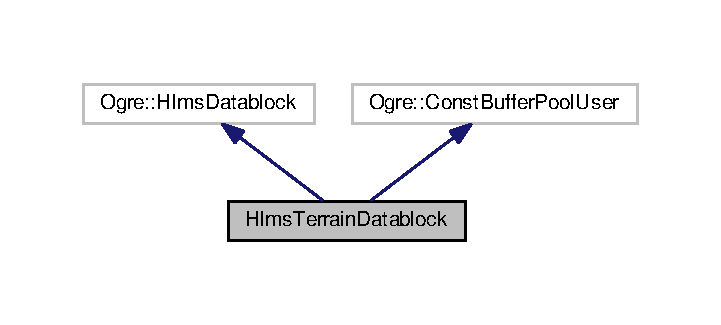
\includegraphics[width=346pt]{class_hlms_terrain_datablock__inherit__graph}
\end{center}
\end{figure}


Collaboration diagram for Hlms\+Terrain\+Datablock\+:\nopagebreak
\begin{figure}[H]
\begin{center}
\leavevmode
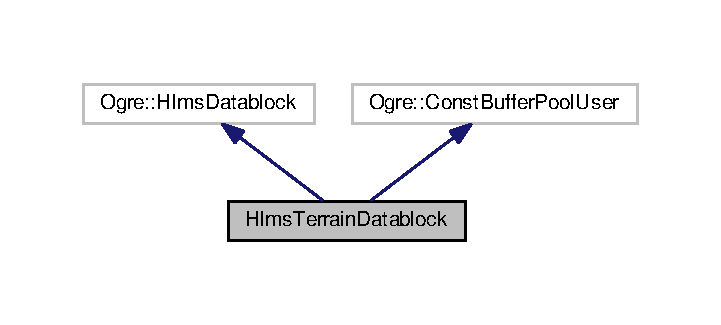
\includegraphics[width=346pt]{class_hlms_terrain_datablock__coll__graph}
\end{center}
\end{figure}
\subsection*{Public Member Functions}
\begin{DoxyCompactItemize}
\item 
\mbox{\Hypertarget{class_hlms_terrain_datablock_af887d30cb63012d835e4a5846067a702}\label{class_hlms_terrain_datablock_af887d30cb63012d835e4a5846067a702}} 
{\bfseries Hlms\+Terrain\+Datablock} (Ogre\+::\+Id\+String name, \hyperlink{class_hlms_terrain}{Hlms\+Terrain} $\ast$creator, const Ogre\+::\+Hlms\+Macroblock $\ast$macroblock, const Ogre\+::\+Hlms\+Blendblock $\ast$blendblock, const Ogre\+::\+Hlms\+Param\+Vec \&params)
\item 
\mbox{\Hypertarget{class_hlms_terrain_datablock_a14ffcf7316b6287560c161cee9d2fb4b}\label{class_hlms_terrain_datablock_a14ffcf7316b6287560c161cee9d2fb4b}} 
void \hyperlink{class_hlms_terrain_datablock_a14ffcf7316b6287560c161cee9d2fb4b}{set\+Diffuse} (const Ogre\+::\+Vector3 \&diffuse\+Colour)
\begin{DoxyCompactList}\small\item\em Sets overall diffuse colour. The colour will be divided by PI for energy conservation. \end{DoxyCompactList}\item 
\mbox{\Hypertarget{class_hlms_terrain_datablock_a97d41acdfe752e5e1fc00f55b78297b3}\label{class_hlms_terrain_datablock_a97d41acdfe752e5e1fc00f55b78297b3}} 
Ogre\+::\+Vector3 {\bfseries get\+Diffuse} (void) const
\item 
\mbox{\Hypertarget{class_hlms_terrain_datablock_a58f763da3ef7027911a76cee7e395095}\label{class_hlms_terrain_datablock_a58f763da3ef7027911a76cee7e395095}} 
void \hyperlink{class_hlms_terrain_datablock_a58f763da3ef7027911a76cee7e395095}{set\+Roughness} (Ogre\+::uint8 detail\+Map\+Idx, float roughness)
\begin{DoxyCompactList}\small\item\em Sets the roughness. \end{DoxyCompactList}\item 
\mbox{\Hypertarget{class_hlms_terrain_datablock_a8db6d139f4f20d16a99d6cff8d5091d8}\label{class_hlms_terrain_datablock_a8db6d139f4f20d16a99d6cff8d5091d8}} 
float {\bfseries get\+Roughness} (Ogre\+::uint8 detail\+Map\+Idx) const
\item 
void \hyperlink{class_hlms_terrain_datablock_acd5e39eb1968ddda8f05d5537fe3f945}{set\+Metalness} (Ogre\+::uint8 detail\+Map\+Idx, float metalness)
\item 
\mbox{\Hypertarget{class_hlms_terrain_datablock_a480b9b9deea9bc4571c80a63e3b0d93a}\label{class_hlms_terrain_datablock_a480b9b9deea9bc4571c80a63e3b0d93a}} 
float {\bfseries get\+Metalness} (Ogre\+::uint8 detail\+Map\+Idx) const
\item 
void \hyperlink{class_hlms_terrain_datablock_a9491ff27ef7052bcce3edb825acc61fe}{\+\_\+set\+Textures} (const \hyperlink{struct_packed_texture}{Packed\+Texture} packed\+Textures\mbox{[}$\,$\mbox{]})
\item 
void \hyperlink{class_hlms_terrain_datablock_a1b27f8fe762d440e239b082b063dccc3}{set\+Texture} (Terrain\+Texture\+Types tex\+Type, Ogre\+::uint16 array\+Index, const Ogre\+::\+Texture\+Ptr \&new\+Texture, const Ogre\+::\+Hlms\+Samplerblock $\ast$ref\+Params=0)
\item 
\mbox{\Hypertarget{class_hlms_terrain_datablock_a47f8cb14b8db112c3a0e0c312d6c9ea4}\label{class_hlms_terrain_datablock_a47f8cb14b8db112c3a0e0c312d6c9ea4}} 
Ogre\+::\+Texture\+Ptr {\bfseries get\+Texture} (Terrain\+Texture\+Types tex\+Type) const
\item 
\mbox{\Hypertarget{class_hlms_terrain_datablock_ac03d887ccfb90caa3926b724c6b40d03}\label{class_hlms_terrain_datablock_ac03d887ccfb90caa3926b724c6b40d03}} 
Ogre\+::\+Texture\+Ptr {\bfseries get\+Texture} (size\+\_\+t tex\+Type) const
\item 
Ogre\+::uint16 \hyperlink{class_hlms_terrain_datablock_af9f5260f2d4238492c9ef2d78e1bc0cb}{\+\_\+get\+Texture\+Idx} (Terrain\+Texture\+Types tex\+Type) const
\item 
void \hyperlink{class_hlms_terrain_datablock_a4e7f40cdd79957bdbfbfd77ecd511c9a}{set\+Samplerblock} (Terrain\+Texture\+Types tex\+Type, const Ogre\+::\+Hlms\+Samplerblock \&params)
\item 
\mbox{\Hypertarget{class_hlms_terrain_datablock_a2744e6ade914ee6235ac06e6aac8d390}\label{class_hlms_terrain_datablock_a2744e6ade914ee6235ac06e6aac8d390}} 
const Ogre\+::\+Hlms\+Samplerblock $\ast$ {\bfseries get\+Samplerblock} (Terrain\+Texture\+Types tex\+Type) const
\item 
void \hyperlink{class_hlms_terrain_datablock_af4b0ac3a3030192a4bb2200567dcc1fd}{set\+Detail\+Map\+Offset\+Scale} (Ogre\+::uint8 detail\+Map, const Ogre\+::\+Vector4 \&offset\+Scale)
\item 
\mbox{\Hypertarget{class_hlms_terrain_datablock_a23befce55b5f98b30a49881ba9fd3262}\label{class_hlms_terrain_datablock_a23befce55b5f98b30a49881ba9fd3262}} 
const Ogre\+::\+Vector4 \& {\bfseries get\+Detail\+Map\+Offset\+Scale} (Ogre\+::uint8 detail\+Map) const
\item 
Ogre\+::uint8 \hyperlink{class_hlms_terrain_datablock_a08b7b8e53cd57ca6729929602d24411a}{get\+Baked\+Texture\+Idx} (Terrain\+Texture\+Types tex\+Type) const
\item 
Ogre\+::uint16 \hyperlink{class_hlms_terrain_datablock_a19f88d8e892a4fbad4f535dcb41387d5}{\+\_\+get\+Texture\+Slice\+Array\+Index} (Terrain\+Texture\+Types tex\+Type) const
\item 
\mbox{\Hypertarget{class_hlms_terrain_datablock_ab8bfdd8fe1881b494d324ed0d1fa07ce}\label{class_hlms_terrain_datablock_ab8bfdd8fe1881b494d324ed0d1fa07ce}} 
virtual void \hyperlink{class_hlms_terrain_datablock_ab8bfdd8fe1881b494d324ed0d1fa07ce}{set\+Alpha\+Test\+Threshold} (float threshold)
\begin{DoxyCompactList}\small\item\em Overloaded to tell it\textquotesingle{}s unsupported. \end{DoxyCompactList}\item 
void \hyperlink{class_hlms_terrain_datablock_ab4d3d4b79e5fa6340579ad40f8be945f}{set\+Brdf} (Terrain\+Brdf\+::\+Terrain\+Brdf brdf)
\item 
\mbox{\Hypertarget{class_hlms_terrain_datablock_a8dbd965218521df0b850e6374ef7867b}\label{class_hlms_terrain_datablock_a8dbd965218521df0b850e6374ef7867b}} 
Ogre\+::uint32 {\bfseries get\+Brdf} (void) const
\item 
\mbox{\Hypertarget{class_hlms_terrain_datablock_acf1639e0c56006527ba33fe0e1809cc6}\label{class_hlms_terrain_datablock_acf1639e0c56006527ba33fe0e1809cc6}} 
virtual void {\bfseries calculate\+Hash} ()
\end{DoxyCompactItemize}
\subsection*{Static Public Member Functions}
\begin{DoxyCompactItemize}
\item 
static Ogre\+::\+Hlms\+Texture\+Manager\+::\+Texture\+Map\+Type \hyperlink{class_hlms_terrain_datablock_a255f81387aab3171b922b9a55fea2647}{suggest\+Map\+Type\+Based\+On\+Texture\+Type} (Terrain\+Texture\+Types type)
\end{DoxyCompactItemize}
\subsection*{Static Public Attributes}
\begin{DoxyCompactItemize}
\item 
\mbox{\Hypertarget{class_hlms_terrain_datablock_ab0dc7e40cc748869c93f9d965dbee085}\label{class_hlms_terrain_datablock_ab0dc7e40cc748869c93f9d965dbee085}} 
static const size\+\_\+t {\bfseries Material\+Size\+In\+Gpu} = 4 $\ast$ 7 $\ast$ 4
\item 
static const size\+\_\+t {\bfseries Material\+Size\+In\+Gpu\+Aligned}
\end{DoxyCompactItemize}
\subsection*{Protected Member Functions}
\begin{DoxyCompactItemize}
\item 
\mbox{\Hypertarget{class_hlms_terrain_datablock_af7a1285a154f1cd2a99fd597644c001e}\label{class_hlms_terrain_datablock_af7a1285a154f1cd2a99fd597644c001e}} 
void {\bfseries schedule\+Const\+Buffer\+Update} (void)
\item 
\mbox{\Hypertarget{class_hlms_terrain_datablock_a45da4dc882095f2090d946c57d609940}\label{class_hlms_terrain_datablock_a45da4dc882095f2090d946c57d609940}} 
virtual void {\bfseries upload\+To\+Const\+Buffer} (char $\ast$dst\+Ptr)
\item 
\mbox{\Hypertarget{class_hlms_terrain_datablock_aa579f6e6f919d9eeb4227751fb908257}\label{class_hlms_terrain_datablock_aa579f6e6f919d9eeb4227751fb908257}} 
Ogre\+::\+Texture\+Ptr \hyperlink{class_hlms_terrain_datablock_aa579f6e6f919d9eeb4227751fb908257}{set\+Texture} (const Ogre\+::\+String \&name, Terrain\+Texture\+Types texture\+Type)
\begin{DoxyCompactList}\small\item\em Sets the appropiate m\+Tex\+Indices\mbox{[}texture\+Type\mbox{]}, and returns the texture pointer. \end{DoxyCompactList}\item 
\mbox{\Hypertarget{class_hlms_terrain_datablock_a4959f9cd0ca5e098017d633f8fafd3f6}\label{class_hlms_terrain_datablock_a4959f9cd0ca5e098017d633f8fafd3f6}} 
void {\bfseries decompile\+Baked\+Textures} (\hyperlink{struct_terrain_baked_texture}{Terrain\+Baked\+Texture} out\+Textures\mbox{[}N\+U\+M\+\_\+\+T\+E\+R\+R\+A\+I\+N\+\_\+\+T\+E\+X\+T\+U\+R\+E\+\_\+\+T\+Y\+P\+ES\mbox{]})
\item 
\mbox{\Hypertarget{class_hlms_terrain_datablock_a5ff1fc63d5778757e66985b5c4379fb2}\label{class_hlms_terrain_datablock_a5ff1fc63d5778757e66985b5c4379fb2}} 
void {\bfseries bake\+Textures} (const \hyperlink{struct_terrain_baked_texture}{Terrain\+Baked\+Texture} textures\mbox{[}N\+U\+M\+\_\+\+T\+E\+R\+R\+A\+I\+N\+\_\+\+T\+E\+X\+T\+U\+R\+E\+\_\+\+T\+Y\+P\+ES\mbox{]})
\end{DoxyCompactItemize}
\subsection*{Protected Attributes}
\begin{DoxyCompactItemize}
\item 
\mbox{\Hypertarget{class_hlms_terrain_datablock_a9899754d640e38f1d0a169ee785ecf13}\label{class_hlms_terrain_datablock_a9899754d640e38f1d0a169ee785ecf13}} 
float {\bfseries mk\+Dr}
\item 
\mbox{\Hypertarget{class_hlms_terrain_datablock_a6ed4b5464a8f78020816c11d666e82ed}\label{class_hlms_terrain_datablock_a6ed4b5464a8f78020816c11d666e82ed}} 
float {\bfseries mk\+Dg}
\item 
\mbox{\Hypertarget{class_hlms_terrain_datablock_ab5865a79503da4fc88243294fd1c6efd}\label{class_hlms_terrain_datablock_ab5865a79503da4fc88243294fd1c6efd}} 
float {\bfseries mk\+Db}
\item 
\mbox{\Hypertarget{class_hlms_terrain_datablock_a09784dfaf2db83084497135642f2712a}\label{class_hlms_terrain_datablock_a09784dfaf2db83084497135642f2712a}} 
float {\bfseries \+\_\+padding0}
\item 
\mbox{\Hypertarget{class_hlms_terrain_datablock_a71460eab8386a86ddf309bcf0d2d63a4}\label{class_hlms_terrain_datablock_a71460eab8386a86ddf309bcf0d2d63a4}} 
float {\bfseries m\+Roughness} \mbox{[}4\mbox{]}
\item 
\mbox{\Hypertarget{class_hlms_terrain_datablock_adbdc33d9934bef8d0c98979521e37227}\label{class_hlms_terrain_datablock_adbdc33d9934bef8d0c98979521e37227}} 
float {\bfseries m\+Metalness} \mbox{[}4\mbox{]}
\item 
\mbox{\Hypertarget{class_hlms_terrain_datablock_a6b678509251519e2d56c6634b14db9c4}\label{class_hlms_terrain_datablock_a6b678509251519e2d56c6634b14db9c4}} 
Ogre\+::\+Vector4 {\bfseries m\+Details\+Offset\+Scale} \mbox{[}4\mbox{]}
\item 
\mbox{\Hypertarget{class_hlms_terrain_datablock_a6d3d2fda15c11659fb396490e05d3b4a}\label{class_hlms_terrain_datablock_a6d3d2fda15c11659fb396490e05d3b4a}} 
Ogre\+::uint16 {\bfseries m\+Tex\+Indices} \mbox{[}N\+U\+M\+\_\+\+T\+E\+R\+R\+A\+I\+N\+\_\+\+T\+E\+X\+T\+U\+R\+E\+\_\+\+T\+Y\+P\+ES\mbox{]}
\item 
\mbox{\Hypertarget{class_hlms_terrain_datablock_a2b7248de99eb1d55a2889a286bb1a6c1}\label{class_hlms_terrain_datablock_a2b7248de99eb1d55a2889a286bb1a6c1}} 
Terrain\+Baked\+Texture\+Array {\bfseries m\+Baked\+Textures}
\item 
Ogre\+::uint8 \hyperlink{class_hlms_terrain_datablock_acb2652e4731f6cf65b232393531b1d11}{m\+Tex\+To\+Baked\+Texture\+Idx} \mbox{[}N\+U\+M\+\_\+\+T\+E\+R\+R\+A\+I\+N\+\_\+\+T\+E\+X\+T\+U\+R\+E\+\_\+\+T\+Y\+P\+ES\mbox{]}
\item 
\mbox{\Hypertarget{class_hlms_terrain_datablock_a7ea68e0c344afb54fa5963f9227a768f}\label{class_hlms_terrain_datablock_a7ea68e0c344afb54fa5963f9227a768f}} 
Ogre\+::\+Hlms\+Samplerblock const  $\ast$ {\bfseries m\+Samplerblocks} \mbox{[}N\+U\+M\+\_\+\+T\+E\+R\+R\+A\+I\+N\+\_\+\+T\+E\+X\+T\+U\+R\+E\+\_\+\+T\+Y\+P\+ES\mbox{]}
\item 
Ogre\+::uint32 \hyperlink{class_hlms_terrain_datablock_aec0c1743fab32d302e794a1149139443}{m\+Brdf}
\end{DoxyCompactItemize}
\subsection*{Friends}
\begin{DoxyCompactItemize}
\item 
\mbox{\Hypertarget{class_hlms_terrain_datablock_aa6bf7069e8c5d0a65a557474ec8dff5d}\label{class_hlms_terrain_datablock_aa6bf7069e8c5d0a65a557474ec8dff5d}} 
class {\bfseries Hlms\+Terrain}
\end{DoxyCompactItemize}


\subsection{Detailed Description}
Contains information needed by T\+E\+R\+RA (Physically Based Shading) for Open\+GL 3+ \& D3\+D11+ 

Definition at line 133 of file Hlms\+Terrain\+Datablock.\+h.



\subsection{Member Function Documentation}
\mbox{\Hypertarget{class_hlms_terrain_datablock_af9f5260f2d4238492c9ef2d78e1bc0cb}\label{class_hlms_terrain_datablock_af9f5260f2d4238492c9ef2d78e1bc0cb}} 
\index{Hlms\+Terrain\+Datablock@{Hlms\+Terrain\+Datablock}!\+\_\+get\+Texture\+Idx@{\+\_\+get\+Texture\+Idx}}
\index{\+\_\+get\+Texture\+Idx@{\+\_\+get\+Texture\+Idx}!Hlms\+Terrain\+Datablock@{Hlms\+Terrain\+Datablock}}
\subsubsection{\texorpdfstring{\+\_\+get\+Texture\+Idx()}{\_getTextureIdx()}}
{\footnotesize\ttfamily Ogre\+::uint16 Hlms\+Terrain\+Datablock\+::\+\_\+get\+Texture\+Idx (\begin{DoxyParamCaption}\item[{Terrain\+Texture\+Types}]{tex\+Type }\end{DoxyParamCaption}) const\hspace{0.3cm}{\ttfamily [inline]}}

Returns the internal index to the array in a texture array. Note\+: If there is no texture assigned to the given tex\+Type, returned value is undefined 

Definition at line 217 of file Hlms\+Terrain\+Datablock.\+h.

\mbox{\Hypertarget{class_hlms_terrain_datablock_a19f88d8e892a4fbad4f535dcb41387d5}\label{class_hlms_terrain_datablock_a19f88d8e892a4fbad4f535dcb41387d5}} 
\index{Hlms\+Terrain\+Datablock@{Hlms\+Terrain\+Datablock}!\+\_\+get\+Texture\+Slice\+Array\+Index@{\+\_\+get\+Texture\+Slice\+Array\+Index}}
\index{\+\_\+get\+Texture\+Slice\+Array\+Index@{\+\_\+get\+Texture\+Slice\+Array\+Index}!Hlms\+Terrain\+Datablock@{Hlms\+Terrain\+Datablock}}
\subsubsection{\texorpdfstring{\+\_\+get\+Texture\+Slice\+Array\+Index()}{\_getTextureSliceArrayIndex()}}
{\footnotesize\ttfamily Ogre\+::uint16 Hlms\+Terrain\+Datablock\+::\+\_\+get\+Texture\+Slice\+Array\+Index (\begin{DoxyParamCaption}\item[{Terrain\+Texture\+Types}]{tex\+Type }\end{DoxyParamCaption}) const}

Returns the index to the slice in the texture array. i.\+e. the shader will perform texture( texture\+Array, vec3( uv.\+xy, get\+Texture\+Slice\+Array\+Index() ) ); If there is no texture, return value is undefined. 

Definition at line 368 of file Hlms\+Terrain\+Datablock.\+cpp.

\mbox{\Hypertarget{class_hlms_terrain_datablock_a9491ff27ef7052bcce3edb825acc61fe}\label{class_hlms_terrain_datablock_a9491ff27ef7052bcce3edb825acc61fe}} 
\index{Hlms\+Terrain\+Datablock@{Hlms\+Terrain\+Datablock}!\+\_\+set\+Textures@{\+\_\+set\+Textures}}
\index{\+\_\+set\+Textures@{\+\_\+set\+Textures}!Hlms\+Terrain\+Datablock@{Hlms\+Terrain\+Datablock}}
\subsubsection{\texorpdfstring{\+\_\+set\+Textures()}{\_setTextures()}}
{\footnotesize\ttfamily void Hlms\+Terrain\+Datablock\+::\+\_\+set\+Textures (\begin{DoxyParamCaption}\item[{const \hyperlink{struct_packed_texture}{Packed\+Texture}}]{packed\+Textures\mbox{[}$\,$\mbox{]} }\end{DoxyParamCaption})}

Advanced function for setting all textures at once, instead of one by one, for performance reasons. 
\begin{DoxyParams}{Parameters}
{\em packed\+Textures} & The reference count in packed\+Textures\mbox{[}i\mbox{]}.samplerblock is assumed to have already been increased prior to calling this function. We will not increase. If null, a default samplerblock will be assigned \\
\hline
\end{DoxyParams}


Definition at line 239 of file Hlms\+Terrain\+Datablock.\+cpp.

\mbox{\Hypertarget{class_hlms_terrain_datablock_a08b7b8e53cd57ca6729929602d24411a}\label{class_hlms_terrain_datablock_a08b7b8e53cd57ca6729929602d24411a}} 
\index{Hlms\+Terrain\+Datablock@{Hlms\+Terrain\+Datablock}!get\+Baked\+Texture\+Idx@{get\+Baked\+Texture\+Idx}}
\index{get\+Baked\+Texture\+Idx@{get\+Baked\+Texture\+Idx}!Hlms\+Terrain\+Datablock@{Hlms\+Terrain\+Datablock}}
\subsubsection{\texorpdfstring{get\+Baked\+Texture\+Idx()}{getBakedTextureIdx()}}
{\footnotesize\ttfamily Ogre\+::uint8 Hlms\+Terrain\+Datablock\+::get\+Baked\+Texture\+Idx (\begin{DoxyParamCaption}\item[{Terrain\+Texture\+Types}]{tex\+Type }\end{DoxyParamCaption}) const}

Returns the index to m\+Baked\+Textures. Returns N\+U\+M\+\_\+\+T\+E\+R\+R\+A\+I\+N\+\_\+\+T\+E\+X\+T\+U\+R\+E\+\_\+\+T\+Y\+P\+ES if there is no texture assigned to tex\+Type 

Definition at line 364 of file Hlms\+Terrain\+Datablock.\+cpp.

\mbox{\Hypertarget{class_hlms_terrain_datablock_ab4d3d4b79e5fa6340579ad40f8be945f}\label{class_hlms_terrain_datablock_ab4d3d4b79e5fa6340579ad40f8be945f}} 
\index{Hlms\+Terrain\+Datablock@{Hlms\+Terrain\+Datablock}!set\+Brdf@{set\+Brdf}}
\index{set\+Brdf@{set\+Brdf}!Hlms\+Terrain\+Datablock@{Hlms\+Terrain\+Datablock}}
\subsubsection{\texorpdfstring{set\+Brdf()}{setBrdf()}}
{\footnotesize\ttfamily void Hlms\+Terrain\+Datablock\+::set\+Brdf (\begin{DoxyParamCaption}\item[{Terrain\+Brdf\+::\+Terrain\+Brdf}]{brdf }\end{DoxyParamCaption})}

Changes the B\+R\+DF in use. Calling this function may trigger an Ogre\+::\+Hlms\+Datablock\+::flush\+Renderables 

Definition at line 381 of file Hlms\+Terrain\+Datablock.\+cpp.

\mbox{\Hypertarget{class_hlms_terrain_datablock_af4b0ac3a3030192a4bb2200567dcc1fd}\label{class_hlms_terrain_datablock_af4b0ac3a3030192a4bb2200567dcc1fd}} 
\index{Hlms\+Terrain\+Datablock@{Hlms\+Terrain\+Datablock}!set\+Detail\+Map\+Offset\+Scale@{set\+Detail\+Map\+Offset\+Scale}}
\index{set\+Detail\+Map\+Offset\+Scale@{set\+Detail\+Map\+Offset\+Scale}!Hlms\+Terrain\+Datablock@{Hlms\+Terrain\+Datablock}}
\subsubsection{\texorpdfstring{set\+Detail\+Map\+Offset\+Scale()}{setDetailMapOffsetScale()}}
{\footnotesize\ttfamily void Hlms\+Terrain\+Datablock\+::set\+Detail\+Map\+Offset\+Scale (\begin{DoxyParamCaption}\item[{Ogre\+::uint8}]{detail\+Map,  }\item[{const Ogre\+::\+Vector4 \&}]{offset\+Scale }\end{DoxyParamCaption})}

Sets the scale and offset of the detail map. \begin{DoxyRemark}{Remarks}
A value of Ogre\+::\+Vector4( 0, 0, 1, 1 ) will cause a flush\+Renderables as we remove the code from the shader. 
\end{DoxyRemark}

\begin{DoxyParams}{Parameters}
{\em detail\+Map} & Value in the range \mbox{[}0; 8) Range \mbox{[}0; 4) affects diffuse maps. Range \mbox{[}4; 8) affects normal maps. \\
\hline
{\em offset\+Scale} & XY = Contains the UV offset. ZW = Constains the UV scale. Default value is Ogre\+::\+Vector4( 0, 0, 1, 1 ) \\
\hline
\end{DoxyParams}


Definition at line 346 of file Hlms\+Terrain\+Datablock.\+cpp.

\mbox{\Hypertarget{class_hlms_terrain_datablock_acd5e39eb1968ddda8f05d5537fe3f945}\label{class_hlms_terrain_datablock_acd5e39eb1968ddda8f05d5537fe3f945}} 
\index{Hlms\+Terrain\+Datablock@{Hlms\+Terrain\+Datablock}!set\+Metalness@{set\+Metalness}}
\index{set\+Metalness@{set\+Metalness}!Hlms\+Terrain\+Datablock@{Hlms\+Terrain\+Datablock}}
\subsubsection{\texorpdfstring{set\+Metalness()}{setMetalness()}}
{\footnotesize\ttfamily void Hlms\+Terrain\+Datablock\+::set\+Metalness (\begin{DoxyParamCaption}\item[{Ogre\+::uint8}]{detail\+Map\+Idx,  }\item[{float}]{metalness }\end{DoxyParamCaption})}

Sets the metalness in a metallic workflow. \begin{DoxyRemark}{Remarks}
Overrides any fresnel value. Should be in Metallic mode. 
\end{DoxyRemark}
\begin{DoxySeeAlso}{See also}
set\+Workflow; 
\end{DoxySeeAlso}

\begin{DoxyParams}{Parameters}
{\em metalness} & Value in range \mbox{[}0; 1\mbox{]} \\
\hline
\end{DoxyParams}


Definition at line 230 of file Hlms\+Terrain\+Datablock.\+cpp.

\mbox{\Hypertarget{class_hlms_terrain_datablock_a4e7f40cdd79957bdbfbfd77ecd511c9a}\label{class_hlms_terrain_datablock_a4e7f40cdd79957bdbfbfd77ecd511c9a}} 
\index{Hlms\+Terrain\+Datablock@{Hlms\+Terrain\+Datablock}!set\+Samplerblock@{set\+Samplerblock}}
\index{set\+Samplerblock@{set\+Samplerblock}!Hlms\+Terrain\+Datablock@{Hlms\+Terrain\+Datablock}}
\subsubsection{\texorpdfstring{set\+Samplerblock()}{setSamplerblock()}}
{\footnotesize\ttfamily void Hlms\+Terrain\+Datablock\+::set\+Samplerblock (\begin{DoxyParamCaption}\item[{Terrain\+Texture\+Types}]{tex\+Type,  }\item[{const Ogre\+::\+Hlms\+Samplerblock \&}]{params }\end{DoxyParamCaption})}

Sets a new sampler block to be associated with the texture (i.\+e. filtering mode, addressing modes, etc). If the samplerblock changes, this function will always trigger a Ogre\+::\+Hlms\+Datablock\+::flush\+Renderables 
\begin{DoxyParams}{Parameters}
{\em tex\+Type} & Type of texture. \\
\hline
{\em params} & The sampler block to use as reference. \\
\hline
\end{DoxyParams}


Definition at line 327 of file Hlms\+Terrain\+Datablock.\+cpp.

\mbox{\Hypertarget{class_hlms_terrain_datablock_a1b27f8fe762d440e239b082b063dccc3}\label{class_hlms_terrain_datablock_a1b27f8fe762d440e239b082b063dccc3}} 
\index{Hlms\+Terrain\+Datablock@{Hlms\+Terrain\+Datablock}!set\+Texture@{set\+Texture}}
\index{set\+Texture@{set\+Texture}!Hlms\+Terrain\+Datablock@{Hlms\+Terrain\+Datablock}}
\subsubsection{\texorpdfstring{set\+Texture()}{setTexture()}}
{\footnotesize\ttfamily void Hlms\+Terrain\+Datablock\+::set\+Texture (\begin{DoxyParamCaption}\item[{Terrain\+Texture\+Types}]{tex\+Type,  }\item[{Ogre\+::uint16}]{array\+Index,  }\item[{const Ogre\+::\+Texture\+Ptr \&}]{new\+Texture,  }\item[{const Ogre\+::\+Hlms\+Samplerblock $\ast$}]{ref\+Params = {\ttfamily 0} }\end{DoxyParamCaption})}

Sets a new texture for rendering. Calling this function may trigger an Ogre\+::\+Hlms\+Datablock\+::flush\+Renderables if the texture or the samplerblock changes. Won\textquotesingle{}t be called if only the array\+Index changes 
\begin{DoxyParams}{Parameters}
{\em tex\+Type} & Type of the texture. \\
\hline
{\em array\+Index} & The index in the array texture. \\
\hline
{\em new\+Texture} & Texture to change to. If it is null and previously wasn\textquotesingle{}t (or viceversa), will trigger Ogre\+::\+Hlms\+Datablock\+::flush\+Renderables. \\
\hline
{\em params} & Optional. We\textquotesingle{}ll create (or retrieve an existing) samplerblock based on the input parameters. When null, we leave the previously set samplerblock (if a texture is being set, and if no samplerblock was set, we\textquotesingle{}ll create a default one) \\
\hline
\end{DoxyParams}


Definition at line 269 of file Hlms\+Terrain\+Datablock.\+cpp.

\mbox{\Hypertarget{class_hlms_terrain_datablock_a255f81387aab3171b922b9a55fea2647}\label{class_hlms_terrain_datablock_a255f81387aab3171b922b9a55fea2647}} 
\index{Hlms\+Terrain\+Datablock@{Hlms\+Terrain\+Datablock}!suggest\+Map\+Type\+Based\+On\+Texture\+Type@{suggest\+Map\+Type\+Based\+On\+Texture\+Type}}
\index{suggest\+Map\+Type\+Based\+On\+Texture\+Type@{suggest\+Map\+Type\+Based\+On\+Texture\+Type}!Hlms\+Terrain\+Datablock@{Hlms\+Terrain\+Datablock}}
\subsubsection{\texorpdfstring{suggest\+Map\+Type\+Based\+On\+Texture\+Type()}{suggestMapTypeBasedOnTextureType()}}
{\footnotesize\ttfamily static Ogre\+::\+Hlms\+Texture\+Manager\+::\+Texture\+Map\+Type Hlms\+Terrain\+Datablock\+::suggest\+Map\+Type\+Based\+On\+Texture\+Type (\begin{DoxyParamCaption}\item[{Terrain\+Texture\+Types}]{type }\end{DoxyParamCaption})\hspace{0.3cm}{\ttfamily [static]}}

Suggests the Texture\+Map\+Type (aka texture category) for each type of texture (i.\+e. normals should load from T\+E\+X\+T\+U\+R\+E\+\_\+\+T\+Y\+P\+E\+\_\+\+N\+O\+R\+M\+A\+LS). \begin{DoxyRemark}{Remarks}
Remember that if \char`\"{}my\+Texture\char`\"{} was loaded as T\+E\+X\+T\+U\+R\+E\+\_\+\+T\+Y\+P\+E\+\_\+\+D\+I\+F\+F\+U\+SE and then you try to load it as T\+E\+X\+T\+U\+R\+E\+\_\+\+T\+Y\+P\+E\+\_\+\+N\+O\+R\+M\+A\+LS, the first one will prevail until it\textquotesingle{}s removed. You could create an alias however, and thus have two copies of the same texture with different loading parameters. 
\end{DoxyRemark}


\subsection{Member Data Documentation}
\mbox{\Hypertarget{class_hlms_terrain_datablock_aec560f7f77c262c7e9aec67ed39f64f4}\label{class_hlms_terrain_datablock_aec560f7f77c262c7e9aec67ed39f64f4}} 
\index{Hlms\+Terrain\+Datablock@{Hlms\+Terrain\+Datablock}!Material\+Size\+In\+Gpu\+Aligned@{Material\+Size\+In\+Gpu\+Aligned}}
\index{Material\+Size\+In\+Gpu\+Aligned@{Material\+Size\+In\+Gpu\+Aligned}!Hlms\+Terrain\+Datablock@{Hlms\+Terrain\+Datablock}}
\subsubsection{\texorpdfstring{Material\+Size\+In\+Gpu\+Aligned}{MaterialSizeInGpuAligned}}
{\footnotesize\ttfamily const size\+\_\+t Hlms\+Terrain\+Datablock\+::\+Material\+Size\+In\+Gpu\+Aligned\hspace{0.3cm}{\ttfamily [static]}}

{\bfseries Initial value\+:}
\begin{DoxyCode}
= Ogre::alignToNextMultiple(
        HlmsTerrainDatablock::MaterialSizeInGpu,
        4 * 4)
\end{DoxyCode}


Definition at line 278 of file Hlms\+Terrain\+Datablock.\+h.

\mbox{\Hypertarget{class_hlms_terrain_datablock_aec0c1743fab32d302e794a1149139443}\label{class_hlms_terrain_datablock_aec0c1743fab32d302e794a1149139443}} 
\index{Hlms\+Terrain\+Datablock@{Hlms\+Terrain\+Datablock}!m\+Brdf@{m\+Brdf}}
\index{m\+Brdf@{m\+Brdf}!Hlms\+Terrain\+Datablock@{Hlms\+Terrain\+Datablock}}
\subsubsection{\texorpdfstring{m\+Brdf}{mBrdf}}
{\footnotesize\ttfamily Ogre\+::uint32 Hlms\+Terrain\+Datablock\+::m\+Brdf\hspace{0.3cm}{\ttfamily [protected]}}

\begin{DoxySeeAlso}{See also}
Terrain\+Brdf\+::\+Terrain\+Brdf 
\end{DoxySeeAlso}


Definition at line 153 of file Hlms\+Terrain\+Datablock.\+h.

\mbox{\Hypertarget{class_hlms_terrain_datablock_acb2652e4731f6cf65b232393531b1d11}\label{class_hlms_terrain_datablock_acb2652e4731f6cf65b232393531b1d11}} 
\index{Hlms\+Terrain\+Datablock@{Hlms\+Terrain\+Datablock}!m\+Tex\+To\+Baked\+Texture\+Idx@{m\+Tex\+To\+Baked\+Texture\+Idx}}
\index{m\+Tex\+To\+Baked\+Texture\+Idx@{m\+Tex\+To\+Baked\+Texture\+Idx}!Hlms\+Terrain\+Datablock@{Hlms\+Terrain\+Datablock}}
\subsubsection{\texorpdfstring{m\+Tex\+To\+Baked\+Texture\+Idx}{mTexToBakedTextureIdx}}
{\footnotesize\ttfamily Ogre\+::uint8 Hlms\+Terrain\+Datablock\+::m\+Tex\+To\+Baked\+Texture\+Idx\mbox{[}N\+U\+M\+\_\+\+T\+E\+R\+R\+A\+I\+N\+\_\+\+T\+E\+X\+T\+U\+R\+E\+\_\+\+T\+Y\+P\+ES\mbox{]}\hspace{0.3cm}{\ttfamily [protected]}}

The way to read this variable is i.\+e. get diffuse texture, m\+Baked\+Textures\mbox{[}m\+Tex\+To\+Baked\+Texture\+Idx\mbox{[}T\+E\+R\+R\+A\+I\+N\+\_\+\+D\+I\+F\+F\+U\+SE\mbox{]}\mbox{]} Then read m\+Tex\+Indices\mbox{[}T\+E\+R\+R\+A\+I\+N\+\_\+\+D\+I\+F\+F\+U\+SE\mbox{]} to know which slice of the texture array. 

Definition at line 148 of file Hlms\+Terrain\+Datablock.\+h.



The documentation for this class was generated from the following files\+:\begin{DoxyCompactItemize}
\item 
/home/louis/projects/\+Le\+Dernier\+Morkid/include/\+Terrain/\+Hlms/Hlms\+Terrain\+Datablock.\+h\item 
/home/louis/projects/\+Le\+Dernier\+Morkid/src/\+Terrain/\+Hlms/Hlms\+Terrain\+Datablock.\+cpp\end{DoxyCompactItemize}

\hypertarget{class_common_1_1_joystick_listener}{}\section{Common\+:\+:Joystick\+Listener Class Reference}
\label{class_common_1_1_joystick_listener}\index{Common\+::\+Joystick\+Listener@{Common\+::\+Joystick\+Listener}}


Inheritance diagram for Common\+:\+:Joystick\+Listener\+:\nopagebreak
\begin{figure}[H]
\begin{center}
\leavevmode
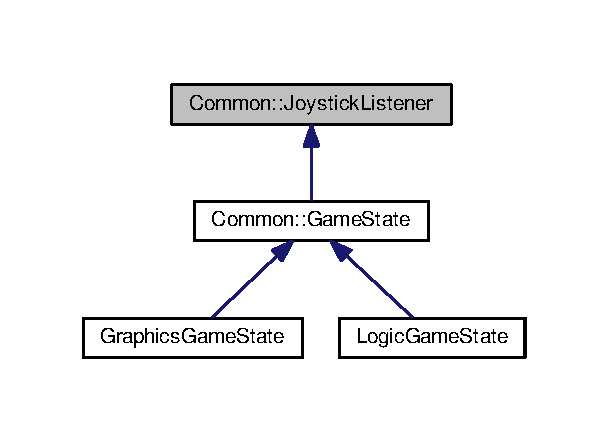
\includegraphics[width=292pt]{class_common_1_1_joystick_listener__inherit__graph}
\end{center}
\end{figure}
\subsection*{Public Member Functions}
\begin{DoxyCompactItemize}
\item 
\mbox{\Hypertarget{class_common_1_1_joystick_listener_a0b1d0c64903a2ac2e5c5f7f8bfb7ce81}\label{class_common_1_1_joystick_listener_a0b1d0c64903a2ac2e5c5f7f8bfb7ce81}} 
virtual void {\bfseries joy\+Button\+Pressed} (const S\+D\+L\+\_\+\+Joy\+Button\+Event \&evt, int button)
\item 
\mbox{\Hypertarget{class_common_1_1_joystick_listener_a9ed8cc90e3644cdbd00355acba3cb1e5}\label{class_common_1_1_joystick_listener_a9ed8cc90e3644cdbd00355acba3cb1e5}} 
virtual void {\bfseries joy\+Button\+Released} (const S\+D\+L\+\_\+\+Joy\+Button\+Event \&evt, int button)
\item 
\mbox{\Hypertarget{class_common_1_1_joystick_listener_ad8cc8de4cab46d53f99c496247ec381e}\label{class_common_1_1_joystick_listener_ad8cc8de4cab46d53f99c496247ec381e}} 
virtual void {\bfseries joy\+Axis\+Moved} (const S\+D\+L\+\_\+\+Joy\+Axis\+Event \&arg, int axis)
\item 
\mbox{\Hypertarget{class_common_1_1_joystick_listener_ac18be87a19beedcd9b93b38849575062}\label{class_common_1_1_joystick_listener_ac18be87a19beedcd9b93b38849575062}} 
virtual void {\bfseries joy\+Pov\+Moved} (const S\+D\+L\+\_\+\+Joy\+Hat\+Event \&arg, int index)
\end{DoxyCompactItemize}


The documentation for this class was generated from the following file\+:\begin{DoxyCompactItemize}
\item 
/home/louis/projects/\+Le\+Dernier\+Morkid/\+Common/include/Input\+Listeners.\+h\end{DoxyCompactItemize}

\hypertarget{class_common_1_1_keyboard_listener}{}\section{Common\+:\+:Keyboard\+Listener Class Reference}
\label{class_common_1_1_keyboard_listener}\index{Common\+::\+Keyboard\+Listener@{Common\+::\+Keyboard\+Listener}}


Simple Listener implementing keyboard functions.  




{\ttfamily \#include $<$Input\+Listeners.\+h$>$}



Inheritance diagram for Common\+:\+:Keyboard\+Listener\+:\nopagebreak
\begin{figure}[H]
\begin{center}
\leavevmode
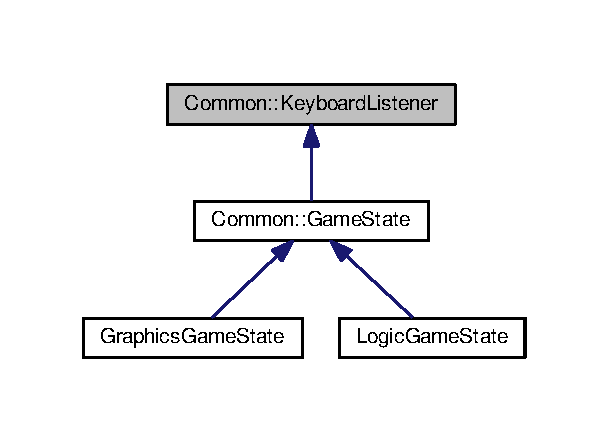
\includegraphics[width=292pt]{class_common_1_1_keyboard_listener__inherit__graph}
\end{center}
\end{figure}
\subsection*{Public Member Functions}
\begin{DoxyCompactItemize}
\item 
\mbox{\Hypertarget{class_common_1_1_keyboard_listener_ac59d0721df35da0d3346b102845a92b2}\label{class_common_1_1_keyboard_listener_ac59d0721df35da0d3346b102845a92b2}} 
virtual void \hyperlink{class_common_1_1_keyboard_listener_ac59d0721df35da0d3346b102845a92b2}{text\+Input} (const S\+D\+L\+\_\+\+Text\+Input\+Event \&arg)
\begin{DoxyCompactList}\small\item\em Function called when text is entered. \end{DoxyCompactList}\item 
\mbox{\Hypertarget{class_common_1_1_keyboard_listener_a1c6fd0d269a2590fcc7c2fa5aca78f5d}\label{class_common_1_1_keyboard_listener_a1c6fd0d269a2590fcc7c2fa5aca78f5d}} 
virtual void \hyperlink{class_common_1_1_keyboard_listener_a1c6fd0d269a2590fcc7c2fa5aca78f5d}{key\+Pressed} (const \hyperlink{struct_s_d_l___keyboard_event}{S\+D\+L\+\_\+\+Keyboard\+Event} \&arg)
\begin{DoxyCompactList}\small\item\em Function called when a key is pressed. \end{DoxyCompactList}\item 
\mbox{\Hypertarget{class_common_1_1_keyboard_listener_a99446142b6d4d6bb230b503afc021e12}\label{class_common_1_1_keyboard_listener_a99446142b6d4d6bb230b503afc021e12}} 
virtual void \hyperlink{class_common_1_1_keyboard_listener_a99446142b6d4d6bb230b503afc021e12}{key\+Released} (const \hyperlink{struct_s_d_l___keyboard_event}{S\+D\+L\+\_\+\+Keyboard\+Event} \&arg)
\begin{DoxyCompactList}\small\item\em Function called when a key is released. \end{DoxyCompactList}\end{DoxyCompactItemize}


\subsection{Detailed Description}
Simple Listener implementing keyboard functions. 

\begin{DoxyRemark}{Remarks}
Does nothing and needs an inheritance 
\end{DoxyRemark}


Definition at line 41 of file Input\+Listeners.\+h.



The documentation for this class was generated from the following file\+:\begin{DoxyCompactItemize}
\item 
/home/louis/projects/\+Le\+Dernier\+Morkid/\+Common/include/Input\+Listeners.\+h\end{DoxyCompactItemize}

\hypertarget{class_le_dernier_morkid}{}\section{Le\+Dernier\+Morkid Class Reference}
\label{class_le_dernier_morkid}\index{Le\+Dernier\+Morkid@{Le\+Dernier\+Morkid}}


Inheritance diagram for Le\+Dernier\+Morkid\+:\nopagebreak
\begin{figure}[H]
\begin{center}
\leavevmode
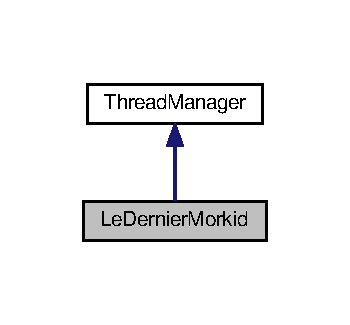
\includegraphics[width=168pt]{class_le_dernier_morkid__inherit__graph}
\end{center}
\end{figure}


Collaboration diagram for Le\+Dernier\+Morkid\+:\nopagebreak
\begin{figure}[H]
\begin{center}
\leavevmode
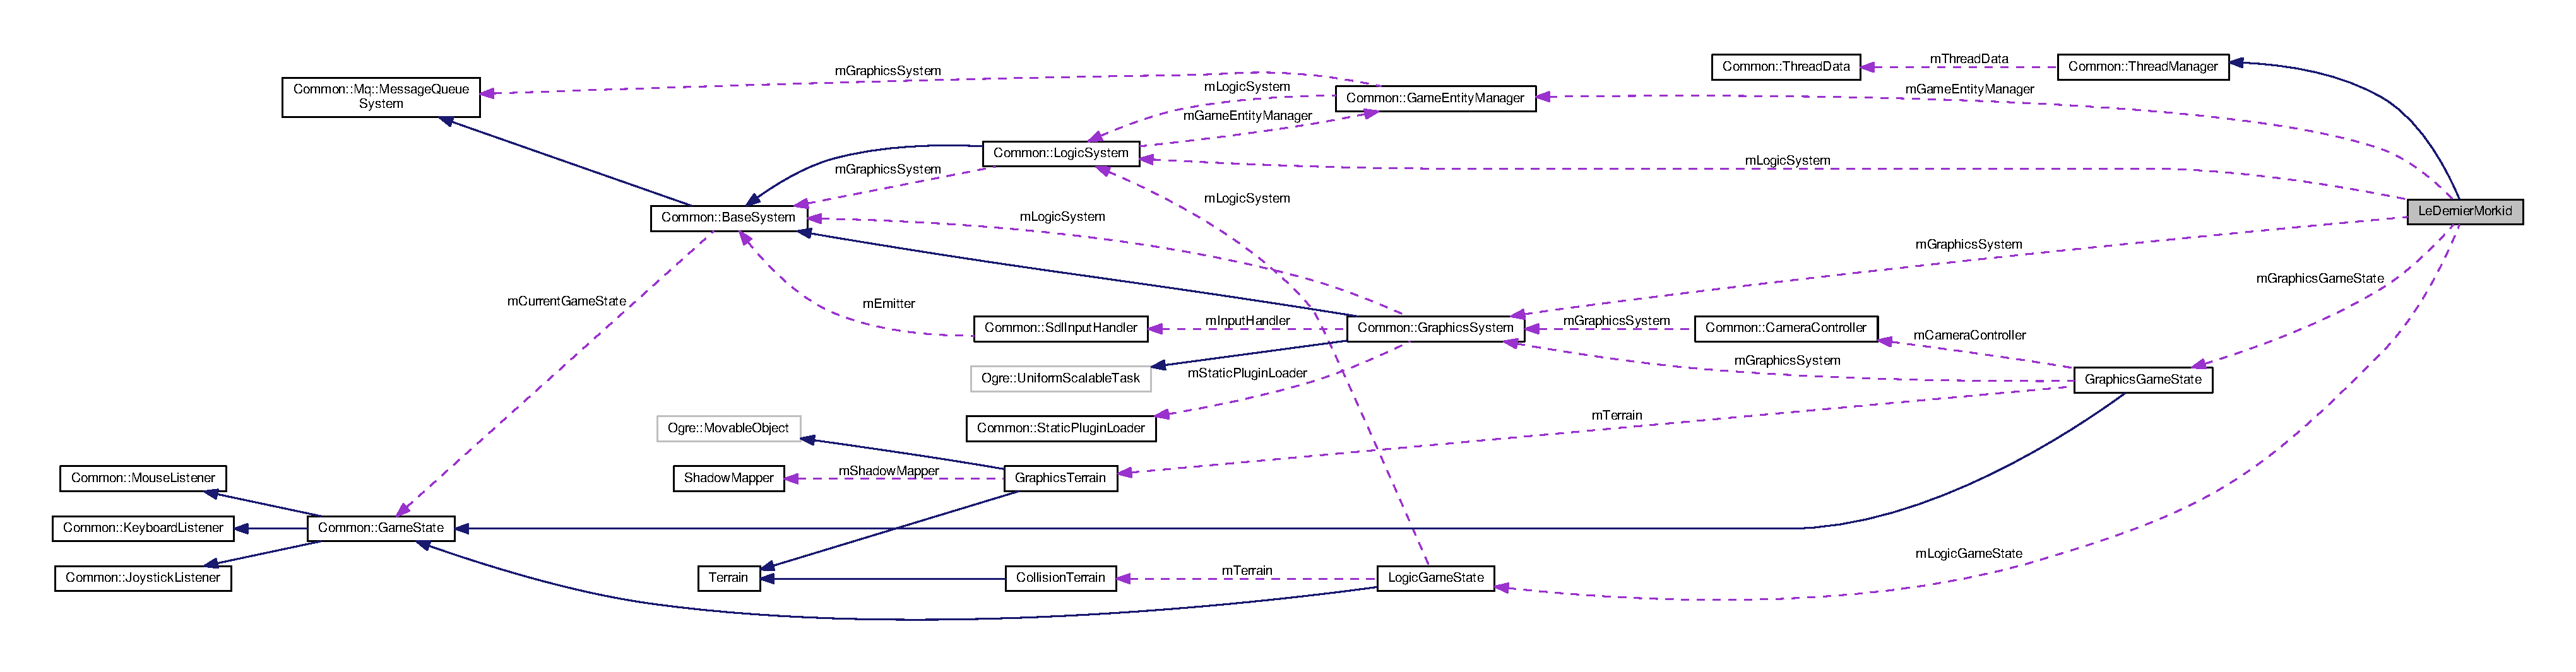
\includegraphics[width=350pt]{class_le_dernier_morkid__coll__graph}
\end{center}
\end{figure}
\subsection*{Classes}
\begin{DoxyCompactItemize}
\item 
struct \hyperlink{struct_le_dernier_morkid_1_1_le_dernier_morkid_thread_data}{Le\+Dernier\+Morkid\+Thread\+Data}
\end{DoxyCompactItemize}
\subsection*{Protected Attributes}
\begin{DoxyCompactItemize}
\item 
\mbox{\Hypertarget{class_le_dernier_morkid_a23be96bb6393f265e43dfb8f264437ae}\label{class_le_dernier_morkid_a23be96bb6393f265e43dfb8f264437ae}} 
\hyperlink{class_graphics_game_state}{Graphics\+Game\+State} $\ast$ {\bfseries m\+Graphics\+Game\+State}
\item 
\mbox{\Hypertarget{class_le_dernier_morkid_af8d20b6c7fab7adcc3d2abadc26fe37d}\label{class_le_dernier_morkid_af8d20b6c7fab7adcc3d2abadc26fe37d}} 
\hyperlink{class_logic_game_state}{Logic\+Game\+State} $\ast$ {\bfseries m\+Logic\+Game\+State}
\item 
\mbox{\Hypertarget{class_le_dernier_morkid_a45fcb3ad212fe7736cb5760e2c33c6e6}\label{class_le_dernier_morkid_a45fcb3ad212fe7736cb5760e2c33c6e6}} 
\hyperlink{class_common_1_1_graphics_system}{Graphics\+System} $\ast$ {\bfseries m\+Graphics\+System}
\item 
\mbox{\Hypertarget{class_le_dernier_morkid_abdf1e8dbee68f3d5aa98f059e0315465}\label{class_le_dernier_morkid_abdf1e8dbee68f3d5aa98f059e0315465}} 
\hyperlink{class_common_1_1_logic_system}{Logic\+System} $\ast$ {\bfseries m\+Logic\+System}
\item 
\mbox{\Hypertarget{class_le_dernier_morkid_a361bc714a10d219778d4f52d1f8cdb63}\label{class_le_dernier_morkid_a361bc714a10d219778d4f52d1f8cdb63}} 
\hyperlink{class_common_1_1_game_entity_manager}{Game\+Entity\+Manager} $\ast$ {\bfseries m\+Game\+Entity\+Manager}
\end{DoxyCompactItemize}
\subsection*{Additional Inherited Members}


The documentation for this class was generated from the following files\+:\begin{DoxyCompactItemize}
\item 
/home/louis/projects/\+Le\+Dernier\+Morkid/include/Le\+Dernier\+Morkid.\+h\item 
/home/louis/projects/\+Le\+Dernier\+Morkid/src/Le\+Dernier\+Morkid.\+cpp\end{DoxyCompactItemize}

\hypertarget{class_le_dernier_morkid_graphics_system}{}\section{Le\+Dernier\+Morkid\+Graphics\+System Class Reference}
\label{class_le_dernier_morkid_graphics_system}\index{Le\+Dernier\+Morkid\+Graphics\+System@{Le\+Dernier\+Morkid\+Graphics\+System}}


Inheritance diagram for Le\+Dernier\+Morkid\+Graphics\+System\+:\nopagebreak
\begin{figure}[H]
\begin{center}
\leavevmode
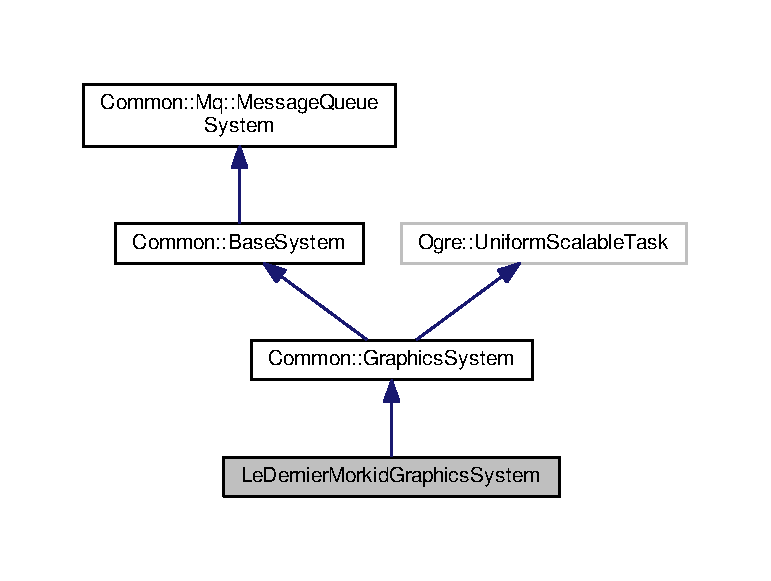
\includegraphics[width=350pt]{class_le_dernier_morkid_graphics_system__inherit__graph}
\end{center}
\end{figure}


Collaboration diagram for Le\+Dernier\+Morkid\+Graphics\+System\+:\nopagebreak
\begin{figure}[H]
\begin{center}
\leavevmode
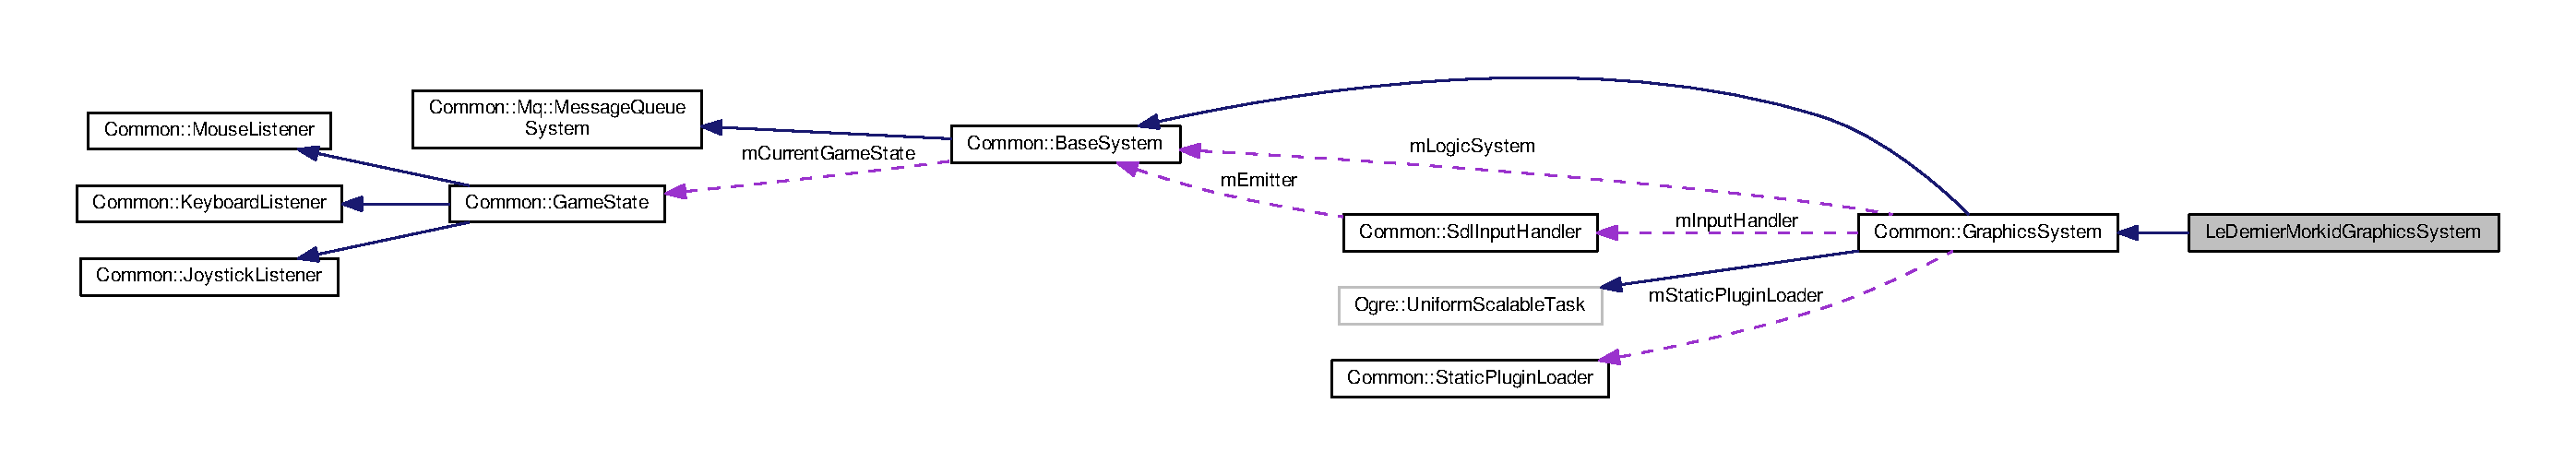
\includegraphics[width=350pt]{class_le_dernier_morkid_graphics_system__coll__graph}
\end{center}
\end{figure}
\subsection*{Public Member Functions}
\begin{DoxyCompactItemize}
\item 
\mbox{\Hypertarget{class_le_dernier_morkid_graphics_system_a99bf6e88562a001af561567044cd4fd3}\label{class_le_dernier_morkid_graphics_system_a99bf6e88562a001af561567044cd4fd3}} 
{\bfseries Le\+Dernier\+Morkid\+Graphics\+System} (\hyperlink{class_graphics_game_state}{Graphics\+Game\+State} $\ast$game\+State, Ogre\+::\+Colour\+Value colour\+Value)
\end{DoxyCompactItemize}
\subsection*{Protected Member Functions}
\begin{DoxyCompactItemize}
\item 
\mbox{\Hypertarget{class_le_dernier_morkid_graphics_system_a3956ef81965b84ec80e1069050cf9c44}\label{class_le_dernier_morkid_graphics_system_a3956ef81965b84ec80e1069050cf9c44}} 
virtual void \hyperlink{class_le_dernier_morkid_graphics_system_a3956ef81965b84ec80e1069050cf9c44}{register\+Hlms} (void)
\begin{DoxyCompactList}\small\item\em Method to register hlms resources. \end{DoxyCompactList}\end{DoxyCompactItemize}
\subsection*{Additional Inherited Members}


\subsection{Detailed Description}


Definition at line 26 of file Le\+Dernier\+Morkid.\+h.



The documentation for this class was generated from the following files\+:\begin{DoxyCompactItemize}
\item 
/home/louis/projects/\+Le\+Dernier\+Morkid/include/Le\+Dernier\+Morkid.\+h\item 
/home/louis/projects/\+Le\+Dernier\+Morkid/src/Le\+Dernier\+Morkid.\+cpp\end{DoxyCompactItemize}

\hypertarget{struct_le_dernier_morkid_1_1_le_dernier_morkid_thread_data}{}\section{Le\+Dernier\+Morkid\+:\+:Le\+Dernier\+Morkid\+Thread\+Data Struct Reference}
\label{struct_le_dernier_morkid_1_1_le_dernier_morkid_thread_data}\index{Le\+Dernier\+Morkid\+::\+Le\+Dernier\+Morkid\+Thread\+Data@{Le\+Dernier\+Morkid\+::\+Le\+Dernier\+Morkid\+Thread\+Data}}


Inheritance diagram for Le\+Dernier\+Morkid\+:\+:Le\+Dernier\+Morkid\+Thread\+Data\+:\nopagebreak
\begin{figure}[H]
\begin{center}
\leavevmode
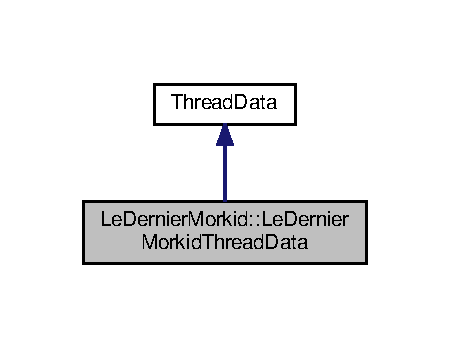
\includegraphics[width=216pt]{struct_le_dernier_morkid_1_1_le_dernier_morkid_thread_data__inherit__graph}
\end{center}
\end{figure}


Collaboration diagram for Le\+Dernier\+Morkid\+:\+:Le\+Dernier\+Morkid\+Thread\+Data\+:\nopagebreak
\begin{figure}[H]
\begin{center}
\leavevmode
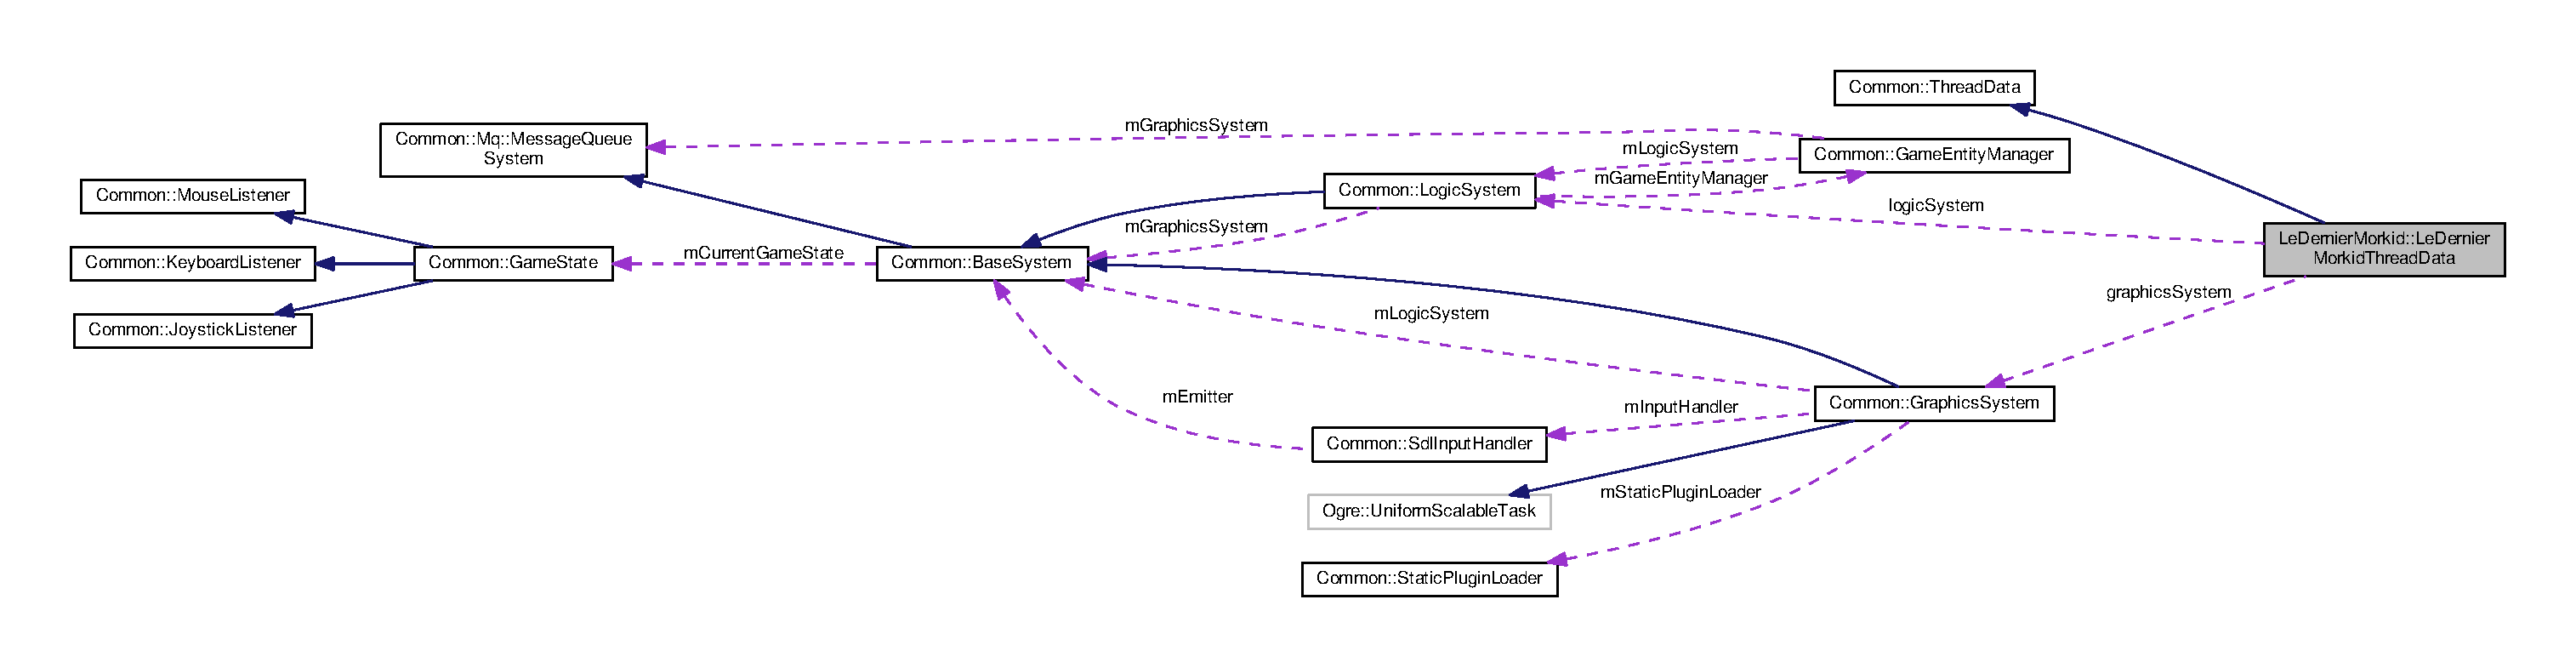
\includegraphics[width=350pt]{struct_le_dernier_morkid_1_1_le_dernier_morkid_thread_data__coll__graph}
\end{center}
\end{figure}
\subsection*{Public Attributes}
\begin{DoxyCompactItemize}
\item 
\mbox{\Hypertarget{struct_le_dernier_morkid_1_1_le_dernier_morkid_thread_data_a14ad8e710579039f8041e3951b33a14d}\label{struct_le_dernier_morkid_1_1_le_dernier_morkid_thread_data_a14ad8e710579039f8041e3951b33a14d}} 
\hyperlink{class_common_1_1_graphics_system}{Graphics\+System} $\ast$ {\bfseries graphics\+System}
\item 
\mbox{\Hypertarget{struct_le_dernier_morkid_1_1_le_dernier_morkid_thread_data_a6e300a8af696aaed836729396ed5f219}\label{struct_le_dernier_morkid_1_1_le_dernier_morkid_thread_data_a6e300a8af696aaed836729396ed5f219}} 
\hyperlink{class_common_1_1_logic_system}{Logic\+System} $\ast$ {\bfseries logic\+System}
\end{DoxyCompactItemize}


The documentation for this struct was generated from the following file\+:\begin{DoxyCompactItemize}
\item 
/home/louis/projects/\+Le\+Dernier\+Morkid/include/Le\+Dernier\+Morkid.\+h\end{DoxyCompactItemize}

\hypertarget{class_logic_game_state}{}\section{Logic\+Game\+State Class Reference}
\label{class_logic_game_state}\index{Logic\+Game\+State@{Logic\+Game\+State}}


Inheritance diagram for Logic\+Game\+State\+:\nopagebreak
\begin{figure}[H]
\begin{center}
\leavevmode
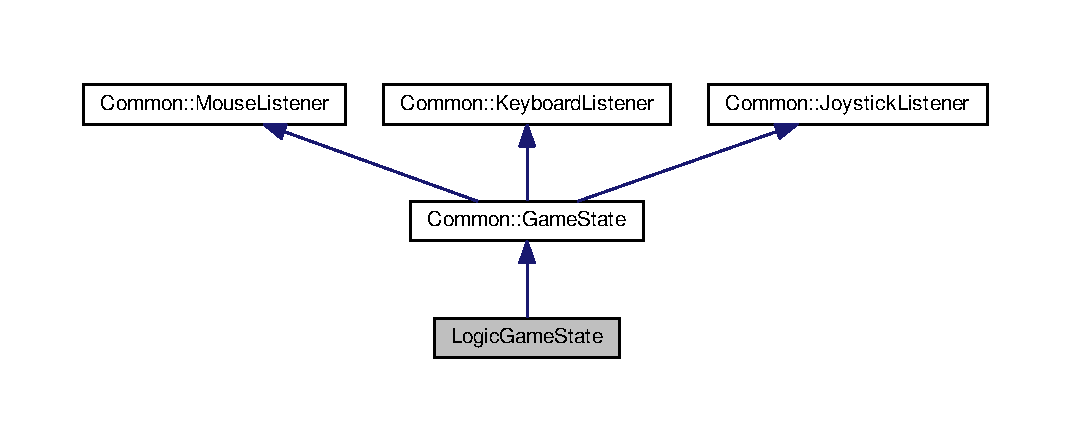
\includegraphics[width=350pt]{class_logic_game_state__inherit__graph}
\end{center}
\end{figure}


Collaboration diagram for Logic\+Game\+State\+:\nopagebreak
\begin{figure}[H]
\begin{center}
\leavevmode
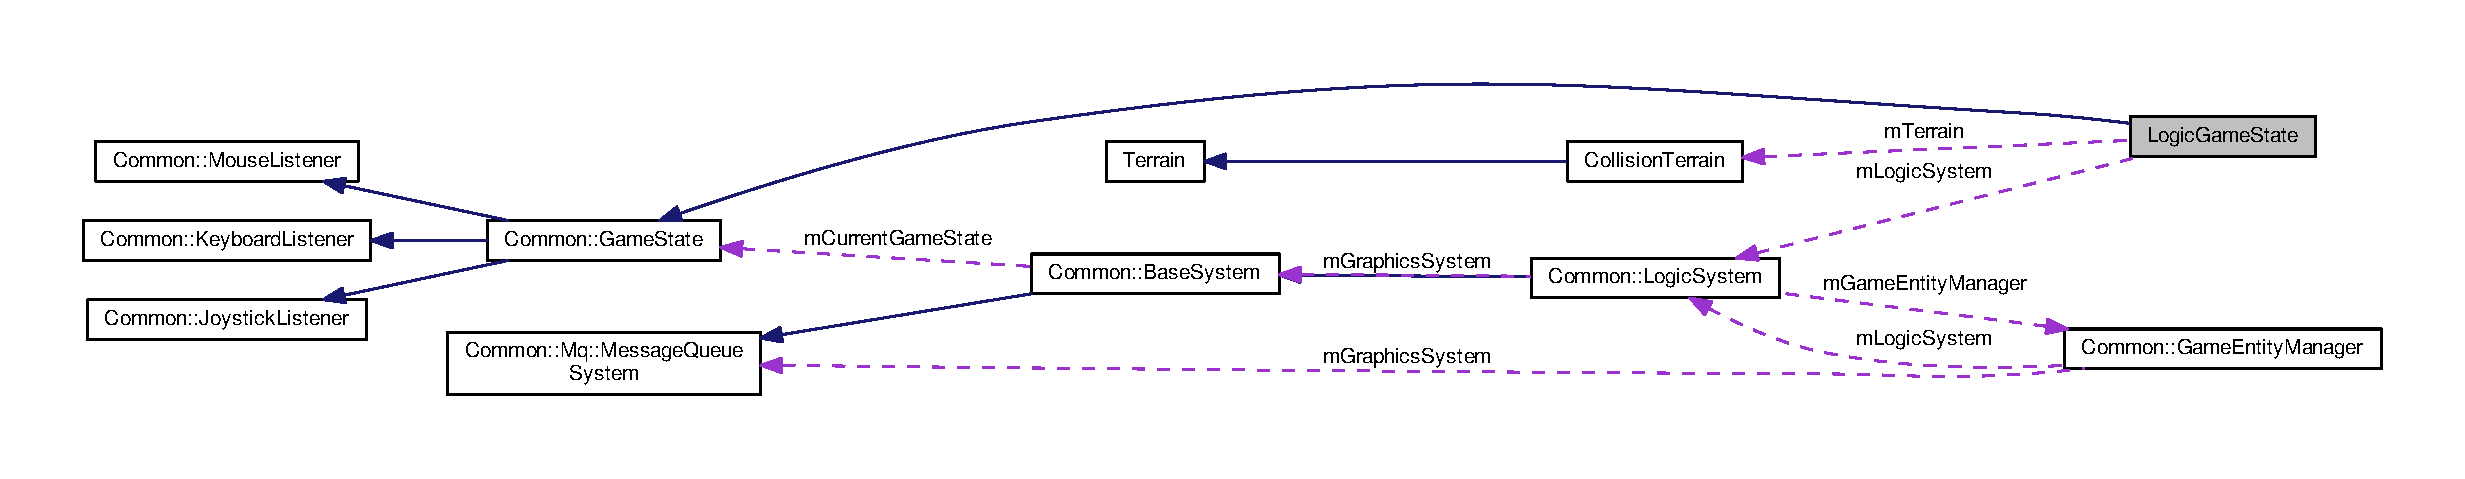
\includegraphics[width=350pt]{class_logic_game_state__coll__graph}
\end{center}
\end{figure}
\subsection*{Public Member Functions}
\begin{DoxyCompactItemize}
\item 
\mbox{\Hypertarget{class_logic_game_state_a769594b36e5668497b9ef0b37dcb4b9b}\label{class_logic_game_state_a769594b36e5668497b9ef0b37dcb4b9b}} 
void {\bfseries \+\_\+notify\+Logic\+System} (\hyperlink{class_common_1_1_logic_system}{Common\+::\+Logic\+System} $\ast$logic\+System)
\item 
\mbox{\Hypertarget{class_logic_game_state_a8ac73ebad7575ebdb5e36fdd59799332}\label{class_logic_game_state_a8ac73ebad7575ebdb5e36fdd59799332}} 
virtual void {\bfseries create\+Scene} (void)
\item 
\mbox{\Hypertarget{class_logic_game_state_a144a2deb659d903956bd955d86c4d6b7}\label{class_logic_game_state_a144a2deb659d903956bd955d86c4d6b7}} 
virtual void {\bfseries update} (float time\+Since\+Last)
\end{DoxyCompactItemize}


The documentation for this class was generated from the following files\+:\begin{DoxyCompactItemize}
\item 
/home/louis/projects/\+Le\+Dernier\+Morkid/include/\+Logic/Logic\+Game\+State.\+h\item 
/home/louis/projects/\+Le\+Dernier\+Morkid/src/\+Logic/Logic\+Game\+State.\+cpp\end{DoxyCompactItemize}

\hypertarget{class_common_1_1_logic_system}{}\section{Common\+:\+:Logic\+System Class Reference}
\label{class_common_1_1_logic_system}\index{Common\+::\+Logic\+System@{Common\+::\+Logic\+System}}


Inheritance diagram for Common\+:\+:Logic\+System\+:\nopagebreak
\begin{figure}[H]
\begin{center}
\leavevmode
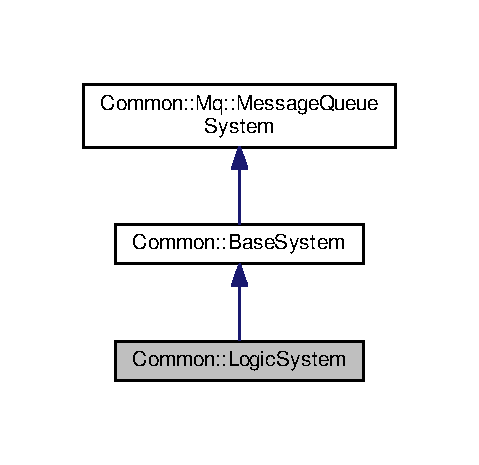
\includegraphics[width=230pt]{class_common_1_1_logic_system__inherit__graph}
\end{center}
\end{figure}


Collaboration diagram for Common\+:\+:Logic\+System\+:\nopagebreak
\begin{figure}[H]
\begin{center}
\leavevmode
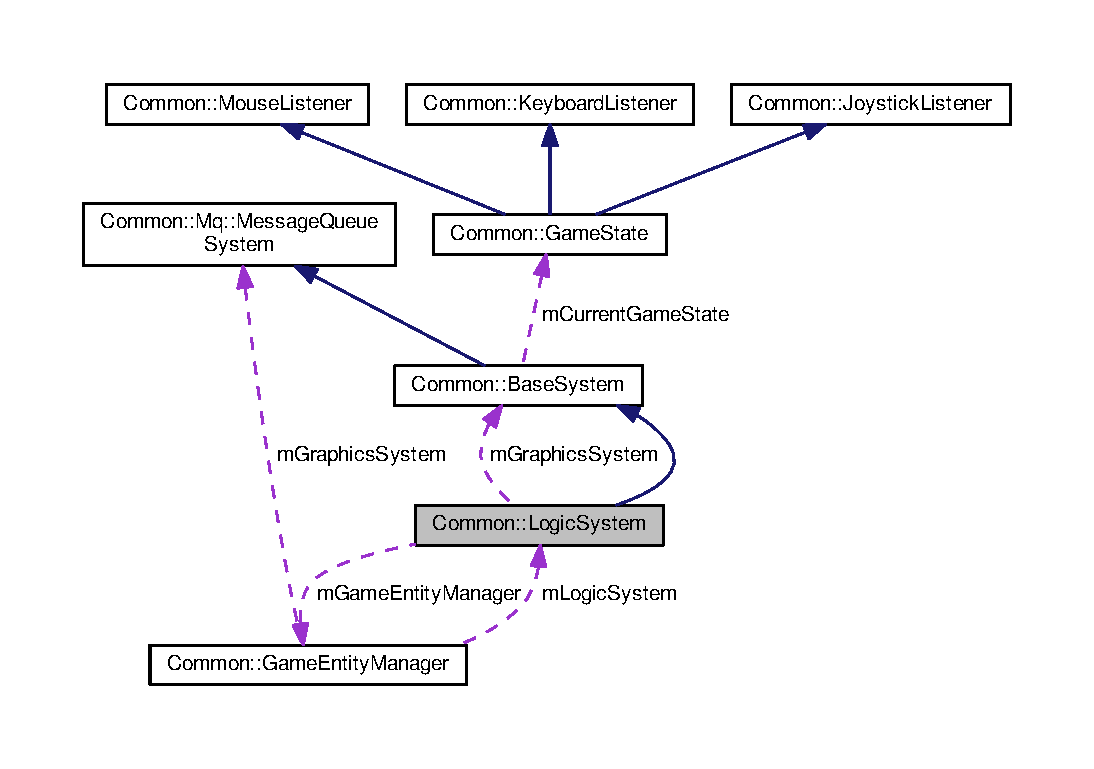
\includegraphics[width=350pt]{class_common_1_1_logic_system__coll__graph}
\end{center}
\end{figure}
\subsection*{Public Member Functions}
\begin{DoxyCompactItemize}
\item 
\mbox{\Hypertarget{class_common_1_1_logic_system_a414d0489e458dea69dd8386fd556acc2}\label{class_common_1_1_logic_system_a414d0489e458dea69dd8386fd556acc2}} 
{\bfseries Logic\+System} (\hyperlink{class_common_1_1_game_state}{Game\+State} $\ast$game\+State)
\item 
\mbox{\Hypertarget{class_common_1_1_logic_system_a6e1389a1e2ed8dd21b46fabdedee5d22}\label{class_common_1_1_logic_system_a6e1389a1e2ed8dd21b46fabdedee5d22}} 
void {\bfseries initialize} ()
\item 
\mbox{\Hypertarget{class_common_1_1_logic_system_a0897460fb4f985b0bd85c2d130b9d585}\label{class_common_1_1_logic_system_a0897460fb4f985b0bd85c2d130b9d585}} 
void {\bfseries \+\_\+notify\+Graphics\+System} (\hyperlink{class_common_1_1_base_system}{Base\+System} $\ast$graphics\+System)
\item 
\mbox{\Hypertarget{class_common_1_1_logic_system_a5eb233fa1e610dbf2b52a76d06ce9782}\label{class_common_1_1_logic_system_a5eb233fa1e610dbf2b52a76d06ce9782}} 
void {\bfseries \+\_\+notify\+Game\+Entity\+Manager} (\hyperlink{class_common_1_1_game_entity_manager}{Game\+Entity\+Manager} $\ast$mgr)
\item 
\mbox{\Hypertarget{class_common_1_1_logic_system_a8f11d71f1f95adbb95dcb6c4281d699a}\label{class_common_1_1_logic_system_a8f11d71f1f95adbb95dcb6c4281d699a}} 
void {\bfseries update} (float time\+Since\+Last)
\item 
\mbox{\Hypertarget{class_common_1_1_logic_system_a4aeed6252b67c4213bd2ba0ca2a6e39c}\label{class_common_1_1_logic_system_a4aeed6252b67c4213bd2ba0ca2a6e39c}} 
void {\bfseries finish\+Frame\+Parallel} (void)
\item 
\mbox{\Hypertarget{class_common_1_1_logic_system_a957d149fb5f02d2d00ec4a4a1827fc2e}\label{class_common_1_1_logic_system_a957d149fb5f02d2d00ec4a4a1827fc2e}} 
\hyperlink{class_common_1_1_game_entity_manager}{Game\+Entity\+Manager} $\ast$ {\bfseries get\+Game\+Entity\+Manager} (void)
\item 
\mbox{\Hypertarget{class_common_1_1_logic_system_a175efaf2f8faf4949e9141cb90a477ce}\label{class_common_1_1_logic_system_a175efaf2f8faf4949e9141cb90a477ce}} 
Ogre\+::uint32 {\bfseries get\+Current\+Transform\+Idx} (void) const
\item 
\mbox{\Hypertarget{class_common_1_1_logic_system_a1172de6e34685a951f956235ca10ca52}\label{class_common_1_1_logic_system_a1172de6e34685a951f956235ca10ca52}} 
bt\+Dynamics\+World $\ast$ {\bfseries get\+World} (void) const
\item 
\mbox{\Hypertarget{class_common_1_1_logic_system_a8ff1976c824aab7d67481390b5e81a4d}\label{class_common_1_1_logic_system_a8ff1976c824aab7d67481390b5e81a4d}} 
void {\bfseries add\+Game\+Entity} (const \hyperlink{struct_common_1_1_game_entity_manager_1_1_created_game_entity}{Game\+Entity\+Manager\+::\+Created\+Game\+Entity} $\ast$cge)
\end{DoxyCompactItemize}
\subsection*{Public Attributes}
\begin{DoxyCompactItemize}
\item 
\mbox{\Hypertarget{class_common_1_1_logic_system_a0b7ac4ad3cc62da7681f649ad6e9823d}\label{class_common_1_1_logic_system_a0b7ac4ad3cc62da7681f649ad6e9823d}} 
\hyperlink{class_common_1_1_base_system}{Base\+System} $\ast$ {\bfseries m\+Graphics\+System}
\end{DoxyCompactItemize}
\subsection*{Protected Member Functions}
\begin{DoxyCompactItemize}
\item 
\mbox{\Hypertarget{class_common_1_1_logic_system_a4495ecadf034103ad58deab6802543fa}\label{class_common_1_1_logic_system_a4495ecadf034103ad58deab6802543fa}} 
virtual void {\bfseries process\+Incoming\+Message} (Mq\+::\+Message\+Id message\+Id, const void $\ast$data)
\end{DoxyCompactItemize}
\subsection*{Protected Attributes}
\begin{DoxyCompactItemize}
\item 
\mbox{\Hypertarget{class_common_1_1_logic_system_a2bd41b9185b04aa8d0cc243dacf07a30}\label{class_common_1_1_logic_system_a2bd41b9185b04aa8d0cc243dacf07a30}} 
\hyperlink{class_common_1_1_game_entity_manager}{Game\+Entity\+Manager} $\ast$ {\bfseries m\+Game\+Entity\+Manager}
\item 
\mbox{\Hypertarget{class_common_1_1_logic_system_a8ff50f813ec112a68298ccf2a44a5a8b}\label{class_common_1_1_logic_system_a8ff50f813ec112a68298ccf2a44a5a8b}} 
bt\+Dynamics\+World $\ast$ {\bfseries m\+World}
\item 
\mbox{\Hypertarget{class_common_1_1_logic_system_af317bbd8f5bda6b3516ced4e575da248}\label{class_common_1_1_logic_system_af317bbd8f5bda6b3516ced4e575da248}} 
bt\+Default\+Collision\+Configuration $\ast$ {\bfseries m\+Collision\+Configuration}
\item 
\mbox{\Hypertarget{class_common_1_1_logic_system_afab3b81f6dd1a32d91a4b2fbe5153fd9}\label{class_common_1_1_logic_system_afab3b81f6dd1a32d91a4b2fbe5153fd9}} 
bt\+Collision\+Dispatcher $\ast$ {\bfseries m\+Dispatcher}
\item 
\mbox{\Hypertarget{class_common_1_1_logic_system_adf97b2bb9e373e9b81e8b52936c5e8d8}\label{class_common_1_1_logic_system_adf97b2bb9e373e9b81e8b52936c5e8d8}} 
bt\+Dbvt\+Broadphase $\ast$ {\bfseries m\+Broadphase}
\item 
\mbox{\Hypertarget{class_common_1_1_logic_system_ab9394f7c8ca427c4121e0445f8ae151d}\label{class_common_1_1_logic_system_ab9394f7c8ca427c4121e0445f8ae151d}} 
bt\+Sequential\+Impulse\+Constraint\+Solver $\ast$ {\bfseries m\+Solver}
\item 
\mbox{\Hypertarget{class_common_1_1_logic_system_a86139251209b2eba41382475544fc41b}\label{class_common_1_1_logic_system_a86139251209b2eba41382475544fc41b}} 
Ogre\+::uint32 {\bfseries m\+Current\+Transform\+Idx}
\item 
\mbox{\Hypertarget{class_common_1_1_logic_system_ae196e1204c52d372075ffa8d15a7548a}\label{class_common_1_1_logic_system_ae196e1204c52d372075ffa8d15a7548a}} 
std\+::deque$<$ Ogre\+::uint32 $>$ {\bfseries m\+Available\+Transform\+Idx}
\end{DoxyCompactItemize}


The documentation for this class was generated from the following files\+:\begin{DoxyCompactItemize}
\item 
/home/louis/projects/\+Le\+Dernier\+Morkid/\+Common/include/Logic\+System.\+h\item 
/home/louis/projects/\+Le\+Dernier\+Morkid/\+Common/src/Logic\+System.\+cpp\end{DoxyCompactItemize}

\hypertarget{class_common_1_1_mq_1_1_message_queue_system}{}\section{Common\+:\+:Mq\+:\+:Message\+Queue\+System Class Reference}
\label{class_common_1_1_mq_1_1_message_queue_system}\index{Common\+::\+Mq\+::\+Message\+Queue\+System@{Common\+::\+Mq\+::\+Message\+Queue\+System}}


Class providing system for threads to communicate.  




{\ttfamily \#include $<$Message\+Queue\+System.\+h$>$}



Inheritance diagram for Common\+:\+:Mq\+:\+:Message\+Queue\+System\+:\nopagebreak
\begin{figure}[H]
\begin{center}
\leavevmode
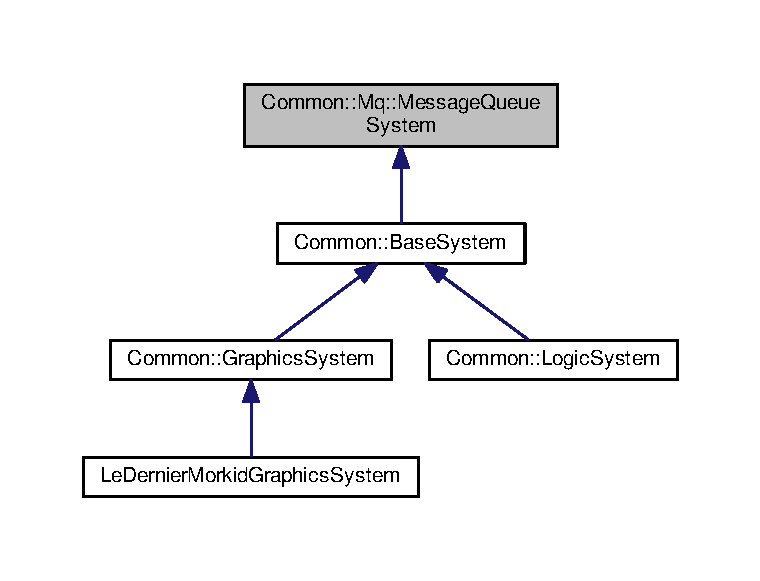
\includegraphics[width=350pt]{class_common_1_1_mq_1_1_message_queue_system__inherit__graph}
\end{center}
\end{figure}
\subsection*{Public Member Functions}
\begin{DoxyCompactItemize}
\item 
\mbox{\Hypertarget{class_common_1_1_mq_1_1_message_queue_system_a0b823b0430b6d72c503ee6dcd72f93d7}\label{class_common_1_1_mq_1_1_message_queue_system_a0b823b0430b6d72c503ee6dcd72f93d7}} 
virtual \hyperlink{class_common_1_1_mq_1_1_message_queue_system_a0b823b0430b6d72c503ee6dcd72f93d7}{$\sim$\+Message\+Queue\+System} ()
\begin{DoxyCompactList}\small\item\em Simple void destructor. \end{DoxyCompactList}\item 
{\footnotesize template$<$typename T $>$ }\\void \hyperlink{class_common_1_1_mq_1_1_message_queue_system_ab9a6196ad22221175ec636ea2b08ec5d}{queue\+Send\+Message} (\hyperlink{class_common_1_1_mq_1_1_message_queue_system}{Message\+Queue\+System} $\ast$dst\+System, \hyperlink{group___common_gaa8c87d2b450282716c906da283e149e6}{Mq\+::\+Message\+Id} message\+Id, const T \&msg)
\item 
void \hyperlink{class_common_1_1_mq_1_1_message_queue_system_a6294a354a094e6ae8fc53e6b936d1963}{flush\+Queued\+Messages} (void)
\item 
{\footnotesize template$<$typename T $>$ }\\void \hyperlink{class_common_1_1_mq_1_1_message_queue_system_a82f4a342971fc840169465d29b78b02f}{receive\+Message\+Immediately} (\hyperlink{group___common_gaa8c87d2b450282716c906da283e149e6}{Mq\+::\+Message\+Id} message\+Id, const T \&msg)
\end{DoxyCompactItemize}
\subsection*{Protected Member Functions}
\begin{DoxyCompactItemize}
\item 
void \hyperlink{class_common_1_1_mq_1_1_message_queue_system_abc956172e5948e71547202f429e5e505}{process\+Incoming\+Messages} (void)
\item 
virtual void \hyperlink{class_common_1_1_mq_1_1_message_queue_system_ad6eb849b72f03e3e4f09c6457c8ecda6}{process\+Incoming\+Message} (\hyperlink{group___common_gaa8c87d2b450282716c906da283e149e6}{Mq\+::\+Message\+Id} message\+Id, const void $\ast$data)=0
\end{DoxyCompactItemize}
\subsection*{Private Types}
\begin{DoxyCompactItemize}
\item 
\mbox{\Hypertarget{class_common_1_1_mq_1_1_message_queue_system_a36ef39384450cb9f027aa9b09ae06034}\label{class_common_1_1_mq_1_1_message_queue_system_a36ef39384450cb9f027aa9b09ae06034}} 
typedef Ogre\+::\+Fast\+Array$<$ unsigned char $>$ {\bfseries Message\+Array}
\item 
\mbox{\Hypertarget{class_common_1_1_mq_1_1_message_queue_system_a0de51c98004bd121fcae2ace2fdb28d7}\label{class_common_1_1_mq_1_1_message_queue_system_a0de51c98004bd121fcae2ace2fdb28d7}} 
typedef std\+::map$<$ \hyperlink{class_common_1_1_mq_1_1_message_queue_system}{Message\+Queue\+System} $\ast$, Message\+Array $>$ {\bfseries Pending\+Message\+Map}
\end{DoxyCompactItemize}
\subsection*{Static Private Member Functions}
\begin{DoxyCompactItemize}
\item 
\mbox{\Hypertarget{class_common_1_1_mq_1_1_message_queue_system_ad92c12ef9927d9534d3575929aef5ec0}\label{class_common_1_1_mq_1_1_message_queue_system_ad92c12ef9927d9534d3575929aef5ec0}} 
{\footnotesize template$<$typename T $>$ }\\static void {\bfseries store\+Message\+To\+Queue} (Message\+Array \&queue, \hyperlink{group___common_gaa8c87d2b450282716c906da283e149e6}{Mq\+::\+Message\+Id} message\+Id, const T \&msg)
\end{DoxyCompactItemize}
\subsection*{Private Attributes}
\begin{DoxyCompactItemize}
\item 
\mbox{\Hypertarget{class_common_1_1_mq_1_1_message_queue_system_aa5491126000d094951d933a780d8c92d}\label{class_common_1_1_mq_1_1_message_queue_system_aa5491126000d094951d933a780d8c92d}} 
Ogre\+::\+Lightweight\+Mutex {\bfseries m\+Message\+Queue\+Mutex}
\item 
\mbox{\Hypertarget{class_common_1_1_mq_1_1_message_queue_system_a987ec96d98e48eb3b8176da9c5c56788}\label{class_common_1_1_mq_1_1_message_queue_system_a987ec96d98e48eb3b8176da9c5c56788}} 
Pending\+Message\+Map {\bfseries m\+Pending\+Outgoing\+Messages}
\item 
\mbox{\Hypertarget{class_common_1_1_mq_1_1_message_queue_system_a98b14d23055f603fbdad7563ce506334}\label{class_common_1_1_mq_1_1_message_queue_system_a98b14d23055f603fbdad7563ce506334}} 
Message\+Array {\bfseries m\+Incoming\+Messages} \mbox{[}2\mbox{]}
\end{DoxyCompactItemize}
\subsection*{Static Private Attributes}
\begin{DoxyCompactItemize}
\item 
\mbox{\Hypertarget{class_common_1_1_mq_1_1_message_queue_system_af72809ed23d11daf72afd93fd34f394e}\label{class_common_1_1_mq_1_1_message_queue_system_af72809ed23d11daf72afd93fd34f394e}} 
static const size\+\_\+t {\bfseries c\+Size\+Of\+Header} = Ogre\+::align\+To\+Next\+Multiple(sizeof(Ogre\+::uint32) $\ast$ 2, sizeof(size\+\_\+t))
\end{DoxyCompactItemize}


\subsection{Detailed Description}
Class providing system for threads to communicate. 

Definition at line 20 of file Message\+Queue\+System.\+h.



\subsection{Member Function Documentation}
\mbox{\Hypertarget{class_common_1_1_mq_1_1_message_queue_system_a6294a354a094e6ae8fc53e6b936d1963}\label{class_common_1_1_mq_1_1_message_queue_system_a6294a354a094e6ae8fc53e6b936d1963}} 
\index{Common\+::\+Mq\+::\+Message\+Queue\+System@{Common\+::\+Mq\+::\+Message\+Queue\+System}!flush\+Queued\+Messages@{flush\+Queued\+Messages}}
\index{flush\+Queued\+Messages@{flush\+Queued\+Messages}!Common\+::\+Mq\+::\+Message\+Queue\+System@{Common\+::\+Mq\+::\+Message\+Queue\+System}}
\subsubsection{\texorpdfstring{flush\+Queued\+Messages()}{flushQueuedMessages()}}
{\footnotesize\ttfamily void Common\+::\+Mq\+::\+Message\+Queue\+System\+::flush\+Queued\+Messages (\begin{DoxyParamCaption}\item[{void}]{ }\end{DoxyParamCaption})\hspace{0.3cm}{\ttfamily [inline]}}

Sends all the messages queued via \hyperlink{class_common_1_1_mq_1_1_message_queue_system_ab9a6196ad22221175ec636ea2b08ec5d}{queue\+Send\+Message()} \begin{DoxyRemark}{Remarks}
Must be called from the thread that owns \textquotesingle{}this\textquotesingle{} 
\end{DoxyRemark}


Definition at line 81 of file Message\+Queue\+System.\+h.

\mbox{\Hypertarget{class_common_1_1_mq_1_1_message_queue_system_ad6eb849b72f03e3e4f09c6457c8ecda6}\label{class_common_1_1_mq_1_1_message_queue_system_ad6eb849b72f03e3e4f09c6457c8ecda6}} 
\index{Common\+::\+Mq\+::\+Message\+Queue\+System@{Common\+::\+Mq\+::\+Message\+Queue\+System}!process\+Incoming\+Message@{process\+Incoming\+Message}}
\index{process\+Incoming\+Message@{process\+Incoming\+Message}!Common\+::\+Mq\+::\+Message\+Queue\+System@{Common\+::\+Mq\+::\+Message\+Queue\+System}}
\subsubsection{\texorpdfstring{process\+Incoming\+Message()}{processIncomingMessage()}}
{\footnotesize\ttfamily virtual void Common\+::\+Mq\+::\+Message\+Queue\+System\+::process\+Incoming\+Message (\begin{DoxyParamCaption}\item[{\hyperlink{group___common_gaa8c87d2b450282716c906da283e149e6}{Mq\+::\+Message\+Id}}]{message\+Id,  }\item[{const void $\ast$}]{data }\end{DoxyParamCaption})\hspace{0.3cm}{\ttfamily [protected]}, {\ttfamily [pure virtual]}}

Method describing the way classes manage the message 
\begin{DoxyParams}{Parameters}
{\em message\+Id} & The Mq\+::\+Message\+Id of the message, used to know what kind of message it is \\
\hline
{\em data} & The data sent with the message, could be anything. Depending on the message\+Id, a conversion will be needed \\
\hline
\end{DoxyParams}
\begin{DoxyRemark}{Remarks}
Derived classes must implement this function to process the incoming message 
\end{DoxyRemark}


Implemented in \hyperlink{class_common_1_1_graphics_system_a8d286a151ed9a65f0eebe1ac119e2d59}{Common\+::\+Graphics\+System}, \hyperlink{class_common_1_1_base_system_a6820dfed1ee63f376e5773b361e3d2a8}{Common\+::\+Base\+System}, and \hyperlink{class_common_1_1_logic_system_a4495ecadf034103ad58deab6802543fa}{Common\+::\+Logic\+System}.

\mbox{\Hypertarget{class_common_1_1_mq_1_1_message_queue_system_abc956172e5948e71547202f429e5e505}\label{class_common_1_1_mq_1_1_message_queue_system_abc956172e5948e71547202f429e5e505}} 
\index{Common\+::\+Mq\+::\+Message\+Queue\+System@{Common\+::\+Mq\+::\+Message\+Queue\+System}!process\+Incoming\+Messages@{process\+Incoming\+Messages}}
\index{process\+Incoming\+Messages@{process\+Incoming\+Messages}!Common\+::\+Mq\+::\+Message\+Queue\+System@{Common\+::\+Mq\+::\+Message\+Queue\+System}}
\subsubsection{\texorpdfstring{process\+Incoming\+Messages()}{processIncomingMessages()}}
{\footnotesize\ttfamily void Common\+::\+Mq\+::\+Message\+Queue\+System\+::process\+Incoming\+Messages (\begin{DoxyParamCaption}\item[{void}]{ }\end{DoxyParamCaption})\hspace{0.3cm}{\ttfamily [inline]}, {\ttfamily [protected]}}

Processes all incoming messages received from other threads. \begin{DoxyRemark}{Remarks}
Should be called from the thread that owns \textquotesingle{}this\textquotesingle{} 
\end{DoxyRemark}


Definition at line 123 of file Message\+Queue\+System.\+h.

\mbox{\Hypertarget{class_common_1_1_mq_1_1_message_queue_system_ab9a6196ad22221175ec636ea2b08ec5d}\label{class_common_1_1_mq_1_1_message_queue_system_ab9a6196ad22221175ec636ea2b08ec5d}} 
\index{Common\+::\+Mq\+::\+Message\+Queue\+System@{Common\+::\+Mq\+::\+Message\+Queue\+System}!queue\+Send\+Message@{queue\+Send\+Message}}
\index{queue\+Send\+Message@{queue\+Send\+Message}!Common\+::\+Mq\+::\+Message\+Queue\+System@{Common\+::\+Mq\+::\+Message\+Queue\+System}}
\subsubsection{\texorpdfstring{queue\+Send\+Message()}{queueSendMessage()}}
{\footnotesize\ttfamily template$<$typename T $>$ \\
void Common\+::\+Mq\+::\+Message\+Queue\+System\+::queue\+Send\+Message (\begin{DoxyParamCaption}\item[{\hyperlink{class_common_1_1_mq_1_1_message_queue_system}{Message\+Queue\+System} $\ast$}]{dst\+System,  }\item[{\hyperlink{group___common_gaa8c87d2b450282716c906da283e149e6}{Mq\+::\+Message\+Id}}]{message\+Id,  }\item[{const T \&}]{msg }\end{DoxyParamCaption})\hspace{0.3cm}{\ttfamily [inline]}}

Queues message \textquotesingle{}msg\textquotesingle{} to be sent to a destination \hyperlink{class_common_1_1_mq_1_1_message_queue_system}{Message\+Queue\+System}. This function {\itshape must} be called from the thread that owns \textquotesingle{}this\textquotesingle{} The \textquotesingle{}dst\+System\textquotesingle{} may live in any other thread. 
\begin{DoxyParams}{Parameters}
{\em dst\+System} & The \hyperlink{class_common_1_1_mq_1_1_message_queue_system}{Message\+Queue\+System} we want to send a message to. \\
\hline
{\em message\+Id} & The type of message sended \\
\hline
{\em msg} & The message itself. Structure must be P\+OD. \\
\hline
\end{DoxyParams}
\begin{DoxyRemark}{Remarks}
The message is not instantely delivered. It will be sent when flush\+Queued\+Messages gets called. 
\end{DoxyRemark}


Definition at line 69 of file Message\+Queue\+System.\+h.

\mbox{\Hypertarget{class_common_1_1_mq_1_1_message_queue_system_a82f4a342971fc840169465d29b78b02f}\label{class_common_1_1_mq_1_1_message_queue_system_a82f4a342971fc840169465d29b78b02f}} 
\index{Common\+::\+Mq\+::\+Message\+Queue\+System@{Common\+::\+Mq\+::\+Message\+Queue\+System}!receive\+Message\+Immediately@{receive\+Message\+Immediately}}
\index{receive\+Message\+Immediately@{receive\+Message\+Immediately}!Common\+::\+Mq\+::\+Message\+Queue\+System@{Common\+::\+Mq\+::\+Message\+Queue\+System}}
\subsubsection{\texorpdfstring{receive\+Message\+Immediately()}{receiveMessageImmediately()}}
{\footnotesize\ttfamily template$<$typename T $>$ \\
void Common\+::\+Mq\+::\+Message\+Queue\+System\+::receive\+Message\+Immediately (\begin{DoxyParamCaption}\item[{\hyperlink{group___common_gaa8c87d2b450282716c906da283e149e6}{Mq\+::\+Message\+Id}}]{message\+Id,  }\item[{const T \&}]{msg }\end{DoxyParamCaption})\hspace{0.3cm}{\ttfamily [inline]}}

Sends a message to \textquotesingle{}this\textquotesingle{} base system immediately. Use it only for time critical messages or if the sender thread doesn\textquotesingle{}t own its own \hyperlink{class_common_1_1_mq_1_1_message_queue_system}{Message\+Queue\+System} class. 
\begin{DoxyParams}{Parameters}
{\em message\+Id} & The type of message sended \\
\hline
{\em msg} & The message itself. Structure must be P\+OD. \\
\hline
\end{DoxyParams}
\begin{DoxyRemark}{Remarks}
Abusing this function can degrade performance as it would perform frequent locking. See queue\+Send\+Message 
\end{DoxyRemark}


Definition at line 111 of file Message\+Queue\+System.\+h.



The documentation for this class was generated from the following files\+:\begin{DoxyCompactItemize}
\item 
/home/louis/projects/\+Le\+Dernier\+Morkid/\+Common/include/\+Threading/Message\+Queue\+System.\+h\item 
/home/louis/projects/\+Le\+Dernier\+Morkid/\+Common/src/\+Threading/Messages\+Queue\+System.\+cpp\end{DoxyCompactItemize}

\hypertarget{class_common_1_1_mouse_listener}{}\section{Common\+:\+:Mouse\+Listener Class Reference}
\label{class_common_1_1_mouse_listener}\index{Common\+::\+Mouse\+Listener@{Common\+::\+Mouse\+Listener}}


Inheritance diagram for Common\+:\+:Mouse\+Listener\+:\nopagebreak
\begin{figure}[H]
\begin{center}
\leavevmode
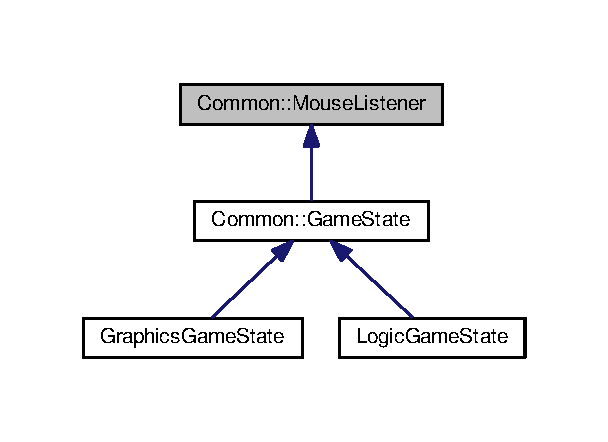
\includegraphics[width=292pt]{class_common_1_1_mouse_listener__inherit__graph}
\end{center}
\end{figure}
\subsection*{Public Member Functions}
\begin{DoxyCompactItemize}
\item 
\mbox{\Hypertarget{class_common_1_1_mouse_listener_a5c61cd1a790d55852a647235371fa5ee}\label{class_common_1_1_mouse_listener_a5c61cd1a790d55852a647235371fa5ee}} 
virtual void {\bfseries mouse\+Moved} (const \hyperlink{union_s_d_l___event}{S\+D\+L\+\_\+\+Event} \&arg)
\item 
\mbox{\Hypertarget{class_common_1_1_mouse_listener_a5b62c0b51cdb3a99ea099c72fb2fa767}\label{class_common_1_1_mouse_listener_a5b62c0b51cdb3a99ea099c72fb2fa767}} 
virtual void {\bfseries mouse\+Pressed} (const \hyperlink{struct_s_d_l___mouse_button_event}{S\+D\+L\+\_\+\+Mouse\+Button\+Event} \&arg, Ogre\+::uint8 id)
\item 
\mbox{\Hypertarget{class_common_1_1_mouse_listener_a820334fbe8a5094938512ebe13965fdc}\label{class_common_1_1_mouse_listener_a820334fbe8a5094938512ebe13965fdc}} 
virtual void {\bfseries mouse\+Released} (const \hyperlink{struct_s_d_l___mouse_button_event}{S\+D\+L\+\_\+\+Mouse\+Button\+Event} \&arg, Ogre\+::uint8 id)
\end{DoxyCompactItemize}


The documentation for this class was generated from the following file\+:\begin{DoxyCompactItemize}
\item 
/home/louis/projects/\+Le\+Dernier\+Morkid/\+Common/include/Input\+Listeners.\+h\end{DoxyCompactItemize}

\hypertarget{struct_common_1_1_movable_object_definition}{}\section{Common\+:\+:Movable\+Object\+Definition Struct Reference}
\label{struct_common_1_1_movable_object_definition}\index{Common\+::\+Movable\+Object\+Definition@{Common\+::\+Movable\+Object\+Definition}}
\subsection*{Public Attributes}
\begin{DoxyCompactItemize}
\item 
\mbox{\Hypertarget{struct_common_1_1_movable_object_definition_a2421cd0320f356ac07de4b53360547a6}\label{struct_common_1_1_movable_object_definition_a2421cd0320f356ac07de4b53360547a6}} 
Ogre\+::\+String {\bfseries mesh\+Name}
\item 
\mbox{\Hypertarget{struct_common_1_1_movable_object_definition_ac43b5c32c8357b59a94201216cd02085}\label{struct_common_1_1_movable_object_definition_ac43b5c32c8357b59a94201216cd02085}} 
Ogre\+::\+String {\bfseries resource\+Group}
\item 
\mbox{\Hypertarget{struct_common_1_1_movable_object_definition_ae7c8198fd708a0f8abe946f42461a691}\label{struct_common_1_1_movable_object_definition_ae7c8198fd708a0f8abe946f42461a691}} 
Ogre\+::\+String\+Vector {\bfseries submesh\+Materials}
\item 
\mbox{\Hypertarget{struct_common_1_1_movable_object_definition_aeb4c2de96c472af36d917cc68fc9e220}\label{struct_common_1_1_movable_object_definition_aeb4c2de96c472af36d917cc68fc9e220}} 
Movable\+Object\+Type {\bfseries mo\+Type}
\end{DoxyCompactItemize}


The documentation for this struct was generated from the following file\+:\begin{DoxyCompactItemize}
\item 
/home/louis/projects/\+Le\+Dernier\+Morkid/\+Common/include/Game\+Entity.\+h\end{DoxyCompactItemize}

\hypertarget{class_collision_1_1_object_state}{}\section{Collision\+:\+:Object\+State Class Reference}
\label{class_collision_1_1_object_state}\index{Collision\+::\+Object\+State@{Collision\+::\+Object\+State}}


Class defines the way Collision and Graphics are synchronized.  




{\ttfamily \#include $<$Object\+State.\+h$>$}



Inheritance diagram for Collision\+:\+:Object\+State\+:\nopagebreak
\begin{figure}[H]
\begin{center}
\leavevmode
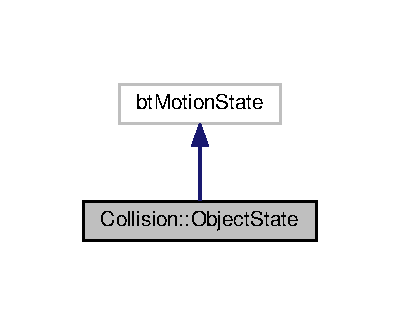
\includegraphics[width=192pt]{class_collision_1_1_object_state__inherit__graph}
\end{center}
\end{figure}


Collaboration diagram for Collision\+:\+:Object\+State\+:\nopagebreak
\begin{figure}[H]
\begin{center}
\leavevmode
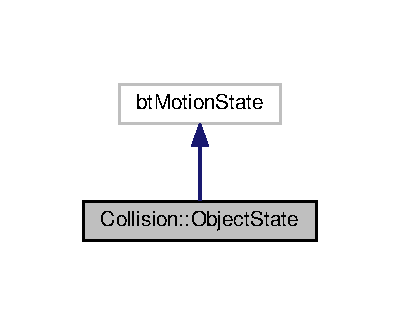
\includegraphics[width=192pt]{class_collision_1_1_object_state__coll__graph}
\end{center}
\end{figure}
\subsection*{Public Member Functions}
\begin{DoxyCompactItemize}
\item 
\hyperlink{class_collision_1_1_object_state_acd780ba908aac6389fc4b22a9257658a}{Object\+State} (bt\+Transform \&initial, \hyperlink{struct_common_1_1_game_entity}{Common\+::\+Game\+Entity} $\ast$game\+Entity, const \hyperlink{class_common_1_1_logic_system}{Common\+::\+Logic\+System} $\ast$logic\+System)
\item 
virtual \hyperlink{class_collision_1_1_object_state_a22a49e4cf7522a2b47fb128af6f65dc6}{$\sim$\+Object\+State} ()
\item 
virtual void \hyperlink{class_collision_1_1_object_state_a2bfa06b1f231cad379fbbd6a86cb9ac9}{get\+World\+Transform} (bt\+Transform \&world\+Trans) const
\item 
virtual void \hyperlink{class_collision_1_1_object_state_a7aeced5d3e1ae27eb7a31f2604ab227c}{set\+World\+Transform} (const bt\+Transform \&world\+Trans)
\end{DoxyCompactItemize}


\subsection{Detailed Description}
Class defines the way Collision and Graphics are synchronized. 

\hyperlink{class_collision_1_1_object_state}{Object\+State} derives from bt\+Motion\+State and overloads the functions to synchronize Ogre\+::\+Scene\+Node and bt\+Rigid\+Body from a \hyperlink{struct_common_1_1_game_entity}{Common\+::\+Game\+Entity}. To use it, do as follow 
\begin{DoxyCode}
rigidBody->setMotionState(\textcolor{keyword}{new} \hyperlink{class_collision_1_1_object_state}{Collision::ObjectState}(transform, gameEntity, 
      logicSystem));
\end{DoxyCode}
 

\subsection{Constructor \& Destructor Documentation}
\mbox{\Hypertarget{class_collision_1_1_object_state_acd780ba908aac6389fc4b22a9257658a}\label{class_collision_1_1_object_state_acd780ba908aac6389fc4b22a9257658a}} 
\index{Collision\+::\+Object\+State@{Collision\+::\+Object\+State}!Object\+State@{Object\+State}}
\index{Object\+State@{Object\+State}!Collision\+::\+Object\+State@{Collision\+::\+Object\+State}}
\subsubsection{\texorpdfstring{Object\+State()}{ObjectState()}}
{\footnotesize\ttfamily Collision\+::\+Object\+State\+::\+Object\+State (\begin{DoxyParamCaption}\item[{bt\+Transform \&}]{initial,  }\item[{\hyperlink{struct_common_1_1_game_entity}{Common\+::\+Game\+Entity} $\ast$}]{game\+Entity,  }\item[{const \hyperlink{class_common_1_1_logic_system}{Common\+::\+Logic\+System} $\ast$}]{logic\+System }\end{DoxyParamCaption})}

Constructor of \hyperlink{class_collision_1_1_collision_camera_controller}{Collision\+Camera\+Controller} 
\begin{DoxyParams}{Parameters}
{\em initial} & the initial transform of the Object \\
\hline
{\em game\+Entity} & the \hyperlink{struct_common_1_1_game_entity}{Common\+::\+Game\+Entity} to synchronize \\
\hline
{\em logic\+System} & the Logic\+System to which belongs the game\+Entity, used to get the transform of the \hyperlink{struct_common_1_1_game_entity}{Common\+::\+Game\+Entity} \\
\hline
\end{DoxyParams}
\mbox{\Hypertarget{class_collision_1_1_object_state_a22a49e4cf7522a2b47fb128af6f65dc6}\label{class_collision_1_1_object_state_a22a49e4cf7522a2b47fb128af6f65dc6}} 
\index{Collision\+::\+Object\+State@{Collision\+::\+Object\+State}!````~Object\+State@{$\sim$\+Object\+State}}
\index{````~Object\+State@{$\sim$\+Object\+State}!Collision\+::\+Object\+State@{Collision\+::\+Object\+State}}
\subsubsection{\texorpdfstring{$\sim$\+Object\+State()}{~ObjectState()}}
{\footnotesize\ttfamily Collision\+::\+Object\+State\+::$\sim$\+Object\+State (\begin{DoxyParamCaption}{ }\end{DoxyParamCaption})\hspace{0.3cm}{\ttfamily [virtual]}}

Simple destructor 

\subsection{Member Function Documentation}
\mbox{\Hypertarget{class_collision_1_1_object_state_a2bfa06b1f231cad379fbbd6a86cb9ac9}\label{class_collision_1_1_object_state_a2bfa06b1f231cad379fbbd6a86cb9ac9}} 
\index{Collision\+::\+Object\+State@{Collision\+::\+Object\+State}!get\+World\+Transform@{get\+World\+Transform}}
\index{get\+World\+Transform@{get\+World\+Transform}!Collision\+::\+Object\+State@{Collision\+::\+Object\+State}}
\subsubsection{\texorpdfstring{get\+World\+Transform()}{getWorldTransform()}}
{\footnotesize\ttfamily void Collision\+::\+Object\+State\+::get\+World\+Transform (\begin{DoxyParamCaption}\item[{bt\+Transform \&}]{world\+Trans }\end{DoxyParamCaption}) const\hspace{0.3cm}{\ttfamily [virtual]}}

Method to get the bt\+Transform of the Object 
\begin{DoxyParams}{Parameters}
{\em world\+Trans} & the bt\+Transform to define with the internal bt\+Transform \\
\hline
\end{DoxyParams}
\begin{DoxyRemark}{Remarks}
This method is used internaly by Bullet. Do not use it 
\end{DoxyRemark}
\mbox{\Hypertarget{class_collision_1_1_object_state_a7aeced5d3e1ae27eb7a31f2604ab227c}\label{class_collision_1_1_object_state_a7aeced5d3e1ae27eb7a31f2604ab227c}} 
\index{Collision\+::\+Object\+State@{Collision\+::\+Object\+State}!set\+World\+Transform@{set\+World\+Transform}}
\index{set\+World\+Transform@{set\+World\+Transform}!Collision\+::\+Object\+State@{Collision\+::\+Object\+State}}
\subsubsection{\texorpdfstring{set\+World\+Transform()}{setWorldTransform()}}
{\footnotesize\ttfamily void Collision\+::\+Object\+State\+::set\+World\+Transform (\begin{DoxyParamCaption}\item[{const bt\+Transform \&}]{world\+Trans }\end{DoxyParamCaption})\hspace{0.3cm}{\ttfamily [virtual]}}

Method to get the bt\+Transform of the Object 
\begin{DoxyParams}{Parameters}
{\em world\+Trans} & the bt\+Transform used to set the internal bt\+Transform \\
\hline
\end{DoxyParams}
\begin{DoxyRemark}{Remarks}
This method is used internaly by Bullet. Do not use it 
\end{DoxyRemark}


The documentation for this class was generated from the following files\+:\begin{DoxyCompactItemize}
\item 
/home/louis/projects/\+Le\+Dernier\+Morkid/\+Collision/include/Object\+State.\+h\item 
/home/louis/projects/\+Le\+Dernier\+Morkid/\+Collision/src/Object\+State.\+cpp\end{DoxyCompactItemize}

\hypertarget{struct_packed_texture}{}\section{Packed\+Texture Struct Reference}
\label{struct_packed_texture}\index{Packed\+Texture@{Packed\+Texture}}


{\ttfamily \#include $<$Hlms\+Terrain\+Datablock.\+h$>$}

\subsection*{Public Attributes}
\begin{DoxyCompactItemize}
\item 
\mbox{\Hypertarget{struct_packed_texture_a95a48d6bd56b3fbefb6897a07dfbac13}\label{struct_packed_texture_a95a48d6bd56b3fbefb6897a07dfbac13}} 
Ogre\+::\+Texture\+Ptr {\bfseries texture}
\item 
\mbox{\Hypertarget{struct_packed_texture_ab79a459476c98fe4455bba13a106dcb1}\label{struct_packed_texture_ab79a459476c98fe4455bba13a106dcb1}} 
Ogre\+::uint16 {\bfseries x\+Idx}
\item 
\mbox{\Hypertarget{struct_packed_texture_a3d790f2867b0a8ac166dbba8860c628d}\label{struct_packed_texture_a3d790f2867b0a8ac166dbba8860c628d}} 
Ogre\+::\+Hlms\+Samplerblock const  $\ast$ {\bfseries samplerblock}
\end{DoxyCompactItemize}


\subsection{Detailed Description}
Used by J\+S\+ON serialization, but can also be used outside of it. \begin{DoxySeeAlso}{See also}
\hyperlink{class_hlms_terrain_datablock_a9491ff27ef7052bcce3edb825acc61fe}{Hlms\+Terrain\+Datablock\+::\+\_\+set\+Textures} 
\end{DoxySeeAlso}


The documentation for this struct was generated from the following file\+:\begin{DoxyCompactItemize}
\item 
/home/louis/projects/\+Le\+Dernier\+Morkid/include/\+Terrain/\+Hlms/Hlms\+Terrain\+Datablock.\+h\end{DoxyCompactItemize}

\hypertarget{struct_hlms_terrain_1_1_pass_data}{}\section{Hlms\+Terrain\+:\+:Pass\+Data Struct Reference}
\label{struct_hlms_terrain_1_1_pass_data}\index{Hlms\+Terrain\+::\+Pass\+Data@{Hlms\+Terrain\+::\+Pass\+Data}}
\subsection*{Public Attributes}
\begin{DoxyCompactItemize}
\item 
\mbox{\Hypertarget{struct_hlms_terrain_1_1_pass_data_ac1e7191cdffc43b7a8adf70203a28f19}\label{struct_hlms_terrain_1_1_pass_data_ac1e7191cdffc43b7a8adf70203a28f19}} 
Ogre\+::\+Fast\+Array$<$ Ogre\+::\+Texture $\ast$ $>$ {\bfseries shadow\+Maps}
\item 
\mbox{\Hypertarget{struct_hlms_terrain_1_1_pass_data_a27dbe70984eb2d8085dd247bd04b0b98}\label{struct_hlms_terrain_1_1_pass_data_a27dbe70984eb2d8085dd247bd04b0b98}} 
Ogre\+::\+Fast\+Array$<$ float $>$ {\bfseries vertex\+Shader\+Shared\+Buffer}
\item 
\mbox{\Hypertarget{struct_hlms_terrain_1_1_pass_data_adfd3b35c0c10cbfe52dca4fb6a216515}\label{struct_hlms_terrain_1_1_pass_data_adfd3b35c0c10cbfe52dca4fb6a216515}} 
Ogre\+::\+Fast\+Array$<$ float $>$ {\bfseries pixel\+Shader\+Shared\+Buffer}
\item 
\mbox{\Hypertarget{struct_hlms_terrain_1_1_pass_data_a698f2e686954dbc8a427cbde28a0d7f1}\label{struct_hlms_terrain_1_1_pass_data_a698f2e686954dbc8a427cbde28a0d7f1}} 
Ogre\+::\+Matrix4 {\bfseries view\+Matrix}
\end{DoxyCompactItemize}


The documentation for this struct was generated from the following file\+:\begin{DoxyCompactItemize}
\item 
/home/louis/projects/\+Le\+Dernier\+Morkid/include/\+Terrain/\+Hlms/Hlms\+Terrain.\+h\end{DoxyCompactItemize}

\hypertarget{struct_pbs_terrain_property}{}\section{Pbs\+Terrain\+Property Struct Reference}
\label{struct_pbs_terrain_property}\index{Pbs\+Terrain\+Property@{Pbs\+Terrain\+Property}}
\subsection*{Static Public Attributes}
\begin{DoxyCompactItemize}
\item 
\mbox{\Hypertarget{struct_pbs_terrain_property_a8fecc53ec81dc75f241a916242417d12}\label{struct_pbs_terrain_property_a8fecc53ec81dc75f241a916242417d12}} 
static const Ogre\+::\+Id\+String {\bfseries Terrain\+Enabled} = Ogre\+::\+Id\+String(\char`\"{}T\+E\+R\+R\+A\+I\+N\+\_\+enabled\char`\"{})
\end{DoxyCompactItemize}


The documentation for this struct was generated from the following files\+:\begin{DoxyCompactItemize}
\item 
/home/louis/projects/\+Le\+Dernier\+Morkid/include/\+Terrain/\+Hlms/\+Pbs\+Listener/Hlms\+Pbs\+Terrain\+Shadows.\+h\item 
/home/louis/projects/\+Le\+Dernier\+Morkid/src/\+Terrain/\+Hlms/\+Pbs\+Listener/Hlms\+Pbs\+Terrain\+Shadows.\+cpp\end{DoxyCompactItemize}

\hypertarget{union_s_d_l___event}{}\section{S\+D\+L\+\_\+\+Event Union Reference}
\label{union_s_d_l___event}\index{S\+D\+L\+\_\+\+Event@{S\+D\+L\+\_\+\+Event}}


Collaboration diagram for S\+D\+L\+\_\+\+Event\+:\nopagebreak
\begin{figure}[H]
\begin{center}
\leavevmode
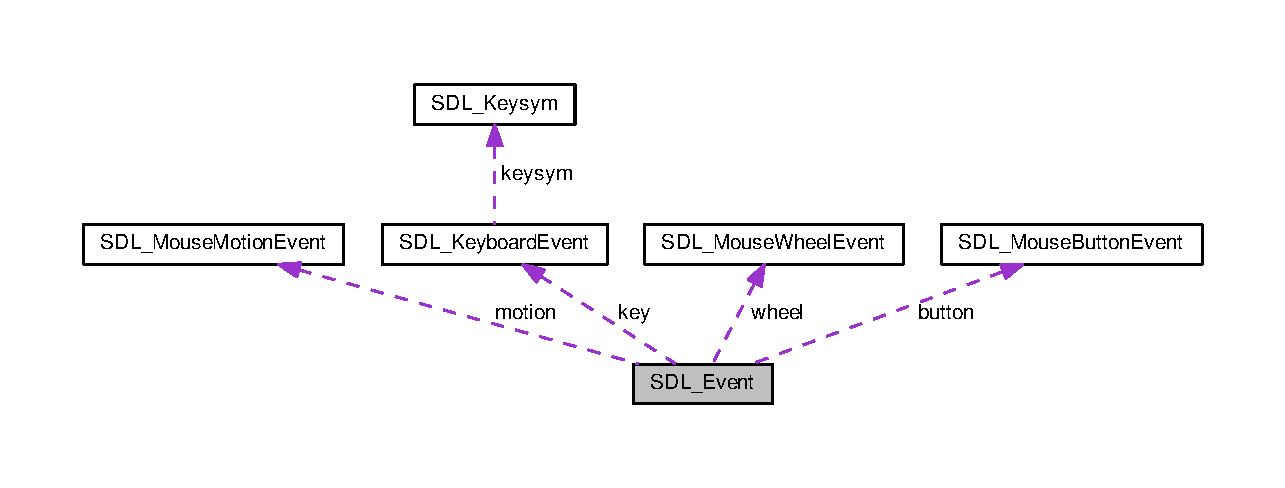
\includegraphics[width=350pt]{union_s_d_l___event__coll__graph}
\end{center}
\end{figure}
\subsection*{Public Attributes}
\begin{DoxyCompactItemize}
\item 
Ogre\+::uint32 \hyperlink{union_s_d_l___event_a8edda577bed999c1c67fec65746637fa}{type}
\item 
\hyperlink{struct_s_d_l___keyboard_event}{S\+D\+L\+\_\+\+Keyboard\+Event} \hyperlink{union_s_d_l___event_ab99927835cc77a9b6bb50b419b4a27df}{key}
\item 
\hyperlink{struct_s_d_l___mouse_motion_event}{S\+D\+L\+\_\+\+Mouse\+Motion\+Event} \hyperlink{union_s_d_l___event_ac3c89e190faacbe84280cd539453bab6}{motion}
\item 
\hyperlink{struct_s_d_l___mouse_button_event}{S\+D\+L\+\_\+\+Mouse\+Button\+Event} \hyperlink{union_s_d_l___event_ab6da2fa2687e5f849f270adecc64785f}{button}
\item 
\hyperlink{struct_s_d_l___mouse_wheel_event}{S\+D\+L\+\_\+\+Mouse\+Wheel\+Event} \hyperlink{union_s_d_l___event_a267d3f550715519ec90a81ccd0e6cbda}{wheel}
\end{DoxyCompactItemize}


\subsection{Member Data Documentation}
\mbox{\Hypertarget{union_s_d_l___event_ab6da2fa2687e5f849f270adecc64785f}\label{union_s_d_l___event_ab6da2fa2687e5f849f270adecc64785f}} 
\index{S\+D\+L\+\_\+\+Event@{S\+D\+L\+\_\+\+Event}!button@{button}}
\index{button@{button}!S\+D\+L\+\_\+\+Event@{S\+D\+L\+\_\+\+Event}}
\subsubsection{\texorpdfstring{button}{button}}
{\footnotesize\ttfamily \hyperlink{struct_s_d_l___mouse_button_event}{S\+D\+L\+\_\+\+Mouse\+Button\+Event} S\+D\+L\+\_\+\+Event\+::button}

Mouse button event data \mbox{\Hypertarget{union_s_d_l___event_ab99927835cc77a9b6bb50b419b4a27df}\label{union_s_d_l___event_ab99927835cc77a9b6bb50b419b4a27df}} 
\index{S\+D\+L\+\_\+\+Event@{S\+D\+L\+\_\+\+Event}!key@{key}}
\index{key@{key}!S\+D\+L\+\_\+\+Event@{S\+D\+L\+\_\+\+Event}}
\subsubsection{\texorpdfstring{key}{key}}
{\footnotesize\ttfamily \hyperlink{struct_s_d_l___keyboard_event}{S\+D\+L\+\_\+\+Keyboard\+Event} S\+D\+L\+\_\+\+Event\+::key}

Keyboard event data \mbox{\Hypertarget{union_s_d_l___event_ac3c89e190faacbe84280cd539453bab6}\label{union_s_d_l___event_ac3c89e190faacbe84280cd539453bab6}} 
\index{S\+D\+L\+\_\+\+Event@{S\+D\+L\+\_\+\+Event}!motion@{motion}}
\index{motion@{motion}!S\+D\+L\+\_\+\+Event@{S\+D\+L\+\_\+\+Event}}
\subsubsection{\texorpdfstring{motion}{motion}}
{\footnotesize\ttfamily \hyperlink{struct_s_d_l___mouse_motion_event}{S\+D\+L\+\_\+\+Mouse\+Motion\+Event} S\+D\+L\+\_\+\+Event\+::motion}

Mouse motion event data \mbox{\Hypertarget{union_s_d_l___event_a8edda577bed999c1c67fec65746637fa}\label{union_s_d_l___event_a8edda577bed999c1c67fec65746637fa}} 
\index{S\+D\+L\+\_\+\+Event@{S\+D\+L\+\_\+\+Event}!type@{type}}
\index{type@{type}!S\+D\+L\+\_\+\+Event@{S\+D\+L\+\_\+\+Event}}
\subsubsection{\texorpdfstring{type}{type}}
{\footnotesize\ttfamily Ogre\+::uint32 S\+D\+L\+\_\+\+Event\+::type}

Event type, shared with all events \mbox{\Hypertarget{union_s_d_l___event_a267d3f550715519ec90a81ccd0e6cbda}\label{union_s_d_l___event_a267d3f550715519ec90a81ccd0e6cbda}} 
\index{S\+D\+L\+\_\+\+Event@{S\+D\+L\+\_\+\+Event}!wheel@{wheel}}
\index{wheel@{wheel}!S\+D\+L\+\_\+\+Event@{S\+D\+L\+\_\+\+Event}}
\subsubsection{\texorpdfstring{wheel}{wheel}}
{\footnotesize\ttfamily \hyperlink{struct_s_d_l___mouse_wheel_event}{S\+D\+L\+\_\+\+Mouse\+Wheel\+Event} S\+D\+L\+\_\+\+Event\+::wheel}

Mouse wheel event data 

The documentation for this union was generated from the following file\+:\begin{DoxyCompactItemize}
\item 
/home/louis/projects/\+Le\+Dernier\+Morkid/\+Common/include/Sdl\+Emulation\+Layer.\+h\end{DoxyCompactItemize}

\hypertarget{struct_s_d_l___keyboard_event}{}\section{S\+D\+L\+\_\+\+Keyboard\+Event Struct Reference}
\label{struct_s_d_l___keyboard_event}\index{S\+D\+L\+\_\+\+Keyboard\+Event@{S\+D\+L\+\_\+\+Keyboard\+Event}}


Collaboration diagram for S\+D\+L\+\_\+\+Keyboard\+Event\+:\nopagebreak
\begin{figure}[H]
\begin{center}
\leavevmode
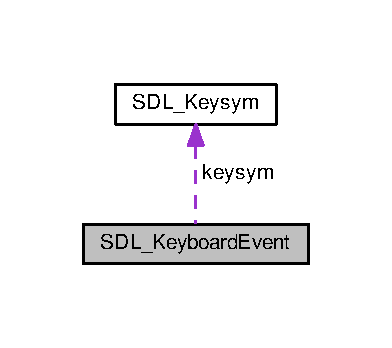
\includegraphics[width=188pt]{struct_s_d_l___keyboard_event__coll__graph}
\end{center}
\end{figure}
\subsection*{Public Attributes}
\begin{DoxyCompactItemize}
\item 
Ogre\+::uint32 \hyperlink{struct_s_d_l___keyboard_event_a1a3eea65c5a9af99bc19f492cbe9ad60}{type}
\item 
\mbox{\Hypertarget{struct_s_d_l___keyboard_event_a40d7efcf7d62dfb549f0b5e81755602c}\label{struct_s_d_l___keyboard_event_a40d7efcf7d62dfb549f0b5e81755602c}} 
Ogre\+::uint32 {\bfseries timestamp}
\item 
Ogre\+::uint32 \hyperlink{struct_s_d_l___keyboard_event_a1f39f22a6dc08d06ddc21ceff061a289}{window\+ID}
\item 
Ogre\+::uint8 \hyperlink{struct_s_d_l___keyboard_event_a54f998fe45b7da252c1aee14e0f80208}{state}
\item 
Ogre\+::uint8 \hyperlink{struct_s_d_l___keyboard_event_a242537ff16ce0a0039d664e4c4d1c40d}{repeat}
\item 
\mbox{\Hypertarget{struct_s_d_l___keyboard_event_ac0940b901240fa603127da42efee8ad9}\label{struct_s_d_l___keyboard_event_ac0940b901240fa603127da42efee8ad9}} 
Ogre\+::uint8 {\bfseries padding2}
\item 
\mbox{\Hypertarget{struct_s_d_l___keyboard_event_a7dc597342fbbc88e20598d6c4e92bc0c}\label{struct_s_d_l___keyboard_event_a7dc597342fbbc88e20598d6c4e92bc0c}} 
Ogre\+::uint8 {\bfseries padding3}
\item 
\hyperlink{struct_s_d_l___keysym}{S\+D\+L\+\_\+\+Keysym} \hyperlink{struct_s_d_l___keyboard_event_a2a57ba820a298f2c02ad5d41fd2b1aa8}{keysym}
\end{DoxyCompactItemize}


\subsection{Member Data Documentation}
\mbox{\Hypertarget{struct_s_d_l___keyboard_event_a2a57ba820a298f2c02ad5d41fd2b1aa8}\label{struct_s_d_l___keyboard_event_a2a57ba820a298f2c02ad5d41fd2b1aa8}} 
\index{S\+D\+L\+\_\+\+Keyboard\+Event@{S\+D\+L\+\_\+\+Keyboard\+Event}!keysym@{keysym}}
\index{keysym@{keysym}!S\+D\+L\+\_\+\+Keyboard\+Event@{S\+D\+L\+\_\+\+Keyboard\+Event}}
\subsubsection{\texorpdfstring{keysym}{keysym}}
{\footnotesize\ttfamily \hyperlink{struct_s_d_l___keysym}{S\+D\+L\+\_\+\+Keysym} S\+D\+L\+\_\+\+Keyboard\+Event\+::keysym}

The key that was pressed or released \mbox{\Hypertarget{struct_s_d_l___keyboard_event_a242537ff16ce0a0039d664e4c4d1c40d}\label{struct_s_d_l___keyboard_event_a242537ff16ce0a0039d664e4c4d1c40d}} 
\index{S\+D\+L\+\_\+\+Keyboard\+Event@{S\+D\+L\+\_\+\+Keyboard\+Event}!repeat@{repeat}}
\index{repeat@{repeat}!S\+D\+L\+\_\+\+Keyboard\+Event@{S\+D\+L\+\_\+\+Keyboard\+Event}}
\subsubsection{\texorpdfstring{repeat}{repeat}}
{\footnotesize\ttfamily Ogre\+::uint8 S\+D\+L\+\_\+\+Keyboard\+Event\+::repeat}

Non-\/zero if this is a key repeat \mbox{\Hypertarget{struct_s_d_l___keyboard_event_a54f998fe45b7da252c1aee14e0f80208}\label{struct_s_d_l___keyboard_event_a54f998fe45b7da252c1aee14e0f80208}} 
\index{S\+D\+L\+\_\+\+Keyboard\+Event@{S\+D\+L\+\_\+\+Keyboard\+Event}!state@{state}}
\index{state@{state}!S\+D\+L\+\_\+\+Keyboard\+Event@{S\+D\+L\+\_\+\+Keyboard\+Event}}
\subsubsection{\texorpdfstring{state}{state}}
{\footnotesize\ttfamily Ogre\+::uint8 S\+D\+L\+\_\+\+Keyboard\+Event\+::state}

\+::\+S\+D\+L\+\_\+\+P\+R\+E\+S\+S\+ED or \+::\+S\+D\+L\+\_\+\+R\+E\+L\+E\+A\+S\+ED \mbox{\Hypertarget{struct_s_d_l___keyboard_event_a1a3eea65c5a9af99bc19f492cbe9ad60}\label{struct_s_d_l___keyboard_event_a1a3eea65c5a9af99bc19f492cbe9ad60}} 
\index{S\+D\+L\+\_\+\+Keyboard\+Event@{S\+D\+L\+\_\+\+Keyboard\+Event}!type@{type}}
\index{type@{type}!S\+D\+L\+\_\+\+Keyboard\+Event@{S\+D\+L\+\_\+\+Keyboard\+Event}}
\subsubsection{\texorpdfstring{type}{type}}
{\footnotesize\ttfamily Ogre\+::uint32 S\+D\+L\+\_\+\+Keyboard\+Event\+::type}

\+::\+S\+D\+L\+\_\+\+K\+E\+Y\+D\+O\+WN or \+::\+S\+D\+L\+\_\+\+K\+E\+Y\+UP \mbox{\Hypertarget{struct_s_d_l___keyboard_event_a1f39f22a6dc08d06ddc21ceff061a289}\label{struct_s_d_l___keyboard_event_a1f39f22a6dc08d06ddc21ceff061a289}} 
\index{S\+D\+L\+\_\+\+Keyboard\+Event@{S\+D\+L\+\_\+\+Keyboard\+Event}!window\+ID@{window\+ID}}
\index{window\+ID@{window\+ID}!S\+D\+L\+\_\+\+Keyboard\+Event@{S\+D\+L\+\_\+\+Keyboard\+Event}}
\subsubsection{\texorpdfstring{window\+ID}{windowID}}
{\footnotesize\ttfamily Ogre\+::uint32 S\+D\+L\+\_\+\+Keyboard\+Event\+::window\+ID}

The window with keyboard focus, if any 

The documentation for this struct was generated from the following file\+:\begin{DoxyCompactItemize}
\item 
/home/louis/projects/\+Le\+Dernier\+Morkid/\+Common/include/Sdl\+Emulation\+Layer.\+h\end{DoxyCompactItemize}

\hypertarget{struct_s_d_l___keysym}{}\section{S\+D\+L\+\_\+\+Keysym Struct Reference}
\label{struct_s_d_l___keysym}\index{S\+D\+L\+\_\+\+Keysym@{S\+D\+L\+\_\+\+Keysym}}
\subsection*{Public Attributes}
\begin{DoxyCompactItemize}
\item 
S\+D\+L\+\_\+\+Scancode \hyperlink{struct_s_d_l___keysym_ad47e9120a511e2efc7ec0c6d8a5ec51e}{scancode}
\item 
S\+D\+L\+\_\+\+Keycode \hyperlink{struct_s_d_l___keysym_a082ff1fd787b79fa6c3a445deb225f08}{sym}
\item 
Ogre\+::uint16 \hyperlink{struct_s_d_l___keysym_a4cbea3e7dd2e50cc57fe05c3af3921fc}{mod}
\item 
\mbox{\Hypertarget{struct_s_d_l___keysym_a423ef40f9956ee0fe3dc9690189461a3}\label{struct_s_d_l___keysym_a423ef40f9956ee0fe3dc9690189461a3}} 
Ogre\+::uint32 {\bfseries unused}
\end{DoxyCompactItemize}


\subsection{Detailed Description}


Definition at line 608 of file Sdl\+Emulation\+Layer.\+h.



\subsection{Member Data Documentation}
\mbox{\Hypertarget{struct_s_d_l___keysym_a4cbea3e7dd2e50cc57fe05c3af3921fc}\label{struct_s_d_l___keysym_a4cbea3e7dd2e50cc57fe05c3af3921fc}} 
\index{S\+D\+L\+\_\+\+Keysym@{S\+D\+L\+\_\+\+Keysym}!mod@{mod}}
\index{mod@{mod}!S\+D\+L\+\_\+\+Keysym@{S\+D\+L\+\_\+\+Keysym}}
\subsubsection{\texorpdfstring{mod}{mod}}
{\footnotesize\ttfamily Ogre\+::uint16 S\+D\+L\+\_\+\+Keysym\+::mod}

current key modifiers 

Definition at line 611 of file Sdl\+Emulation\+Layer.\+h.

\mbox{\Hypertarget{struct_s_d_l___keysym_ad47e9120a511e2efc7ec0c6d8a5ec51e}\label{struct_s_d_l___keysym_ad47e9120a511e2efc7ec0c6d8a5ec51e}} 
\index{S\+D\+L\+\_\+\+Keysym@{S\+D\+L\+\_\+\+Keysym}!scancode@{scancode}}
\index{scancode@{scancode}!S\+D\+L\+\_\+\+Keysym@{S\+D\+L\+\_\+\+Keysym}}
\subsubsection{\texorpdfstring{scancode}{scancode}}
{\footnotesize\ttfamily S\+D\+L\+\_\+\+Scancode S\+D\+L\+\_\+\+Keysym\+::scancode}

S\+DL physical key code -\/ see \+::\+S\+D\+L\+\_\+\+Scancode for details 

Definition at line 609 of file Sdl\+Emulation\+Layer.\+h.

\mbox{\Hypertarget{struct_s_d_l___keysym_a082ff1fd787b79fa6c3a445deb225f08}\label{struct_s_d_l___keysym_a082ff1fd787b79fa6c3a445deb225f08}} 
\index{S\+D\+L\+\_\+\+Keysym@{S\+D\+L\+\_\+\+Keysym}!sym@{sym}}
\index{sym@{sym}!S\+D\+L\+\_\+\+Keysym@{S\+D\+L\+\_\+\+Keysym}}
\subsubsection{\texorpdfstring{sym}{sym}}
{\footnotesize\ttfamily S\+D\+L\+\_\+\+Keycode S\+D\+L\+\_\+\+Keysym\+::sym}

S\+DL virtual key code -\/ see \+::\+S\+D\+L\+\_\+\+Keycode for details 

Definition at line 610 of file Sdl\+Emulation\+Layer.\+h.



The documentation for this struct was generated from the following file\+:\begin{DoxyCompactItemize}
\item 
/home/louis/projects/\+Le\+Dernier\+Morkid/\+Common/include/Sdl\+Emulation\+Layer.\+h\end{DoxyCompactItemize}

\hypertarget{struct_s_d_l___mouse_button_event}{}\section{S\+D\+L\+\_\+\+Mouse\+Button\+Event Struct Reference}
\label{struct_s_d_l___mouse_button_event}\index{S\+D\+L\+\_\+\+Mouse\+Button\+Event@{S\+D\+L\+\_\+\+Mouse\+Button\+Event}}
\subsection*{Public Attributes}
\begin{DoxyCompactItemize}
\item 
Ogre\+::uint32 \hyperlink{struct_s_d_l___mouse_button_event_a07300180f63abeecc56b0358525b096e}{type}
\item 
\mbox{\Hypertarget{struct_s_d_l___mouse_button_event_a8fa7ed510a9dbe6fa8380ee2d3366e08}\label{struct_s_d_l___mouse_button_event_a8fa7ed510a9dbe6fa8380ee2d3366e08}} 
Ogre\+::uint32 {\bfseries timestamp}
\item 
Ogre\+::uint32 \hyperlink{struct_s_d_l___mouse_button_event_a41a4397c3620630c895d6be7a17090bd}{window\+ID}
\item 
Ogre\+::uint32 \hyperlink{struct_s_d_l___mouse_button_event_af4fca7a7a624a906d9afae4316de199d}{which}
\item 
Ogre\+::uint8 \hyperlink{struct_s_d_l___mouse_button_event_ad6da062cd45b2482193e7faac482ca20}{button}
\item 
Ogre\+::uint8 \hyperlink{struct_s_d_l___mouse_button_event_a8d000517d2f23e7577e35bb8c0ef803a}{state}
\item 
Ogre\+::uint8 \hyperlink{struct_s_d_l___mouse_button_event_a35097491b084107fccb5cc014361d3d6}{clicks}
\item 
\mbox{\Hypertarget{struct_s_d_l___mouse_button_event_a2b7ee1562f759ffcc415fb34c03a31a0}\label{struct_s_d_l___mouse_button_event_a2b7ee1562f759ffcc415fb34c03a31a0}} 
Ogre\+::uint8 {\bfseries padding1}
\item 
Ogre\+::int32 \hyperlink{struct_s_d_l___mouse_button_event_aeb46064b59c44d7432356d9323e6c877}{x}
\item 
Ogre\+::int32 \hyperlink{struct_s_d_l___mouse_button_event_a811a7cc2e78a8740efed1bc6bb316819}{y}
\end{DoxyCompactItemize}


\subsection{Detailed Description}


Definition at line 638 of file Sdl\+Emulation\+Layer.\+h.



\subsection{Member Data Documentation}
\mbox{\Hypertarget{struct_s_d_l___mouse_button_event_ad6da062cd45b2482193e7faac482ca20}\label{struct_s_d_l___mouse_button_event_ad6da062cd45b2482193e7faac482ca20}} 
\index{S\+D\+L\+\_\+\+Mouse\+Button\+Event@{S\+D\+L\+\_\+\+Mouse\+Button\+Event}!button@{button}}
\index{button@{button}!S\+D\+L\+\_\+\+Mouse\+Button\+Event@{S\+D\+L\+\_\+\+Mouse\+Button\+Event}}
\subsubsection{\texorpdfstring{button}{button}}
{\footnotesize\ttfamily Ogre\+::uint8 S\+D\+L\+\_\+\+Mouse\+Button\+Event\+::button}

The mouse button index 

Definition at line 643 of file Sdl\+Emulation\+Layer.\+h.

\mbox{\Hypertarget{struct_s_d_l___mouse_button_event_a35097491b084107fccb5cc014361d3d6}\label{struct_s_d_l___mouse_button_event_a35097491b084107fccb5cc014361d3d6}} 
\index{S\+D\+L\+\_\+\+Mouse\+Button\+Event@{S\+D\+L\+\_\+\+Mouse\+Button\+Event}!clicks@{clicks}}
\index{clicks@{clicks}!S\+D\+L\+\_\+\+Mouse\+Button\+Event@{S\+D\+L\+\_\+\+Mouse\+Button\+Event}}
\subsubsection{\texorpdfstring{clicks}{clicks}}
{\footnotesize\ttfamily Ogre\+::uint8 S\+D\+L\+\_\+\+Mouse\+Button\+Event\+::clicks}

1 for single-\/click, 2 for double-\/click, etc. 

Definition at line 645 of file Sdl\+Emulation\+Layer.\+h.

\mbox{\Hypertarget{struct_s_d_l___mouse_button_event_a8d000517d2f23e7577e35bb8c0ef803a}\label{struct_s_d_l___mouse_button_event_a8d000517d2f23e7577e35bb8c0ef803a}} 
\index{S\+D\+L\+\_\+\+Mouse\+Button\+Event@{S\+D\+L\+\_\+\+Mouse\+Button\+Event}!state@{state}}
\index{state@{state}!S\+D\+L\+\_\+\+Mouse\+Button\+Event@{S\+D\+L\+\_\+\+Mouse\+Button\+Event}}
\subsubsection{\texorpdfstring{state}{state}}
{\footnotesize\ttfamily Ogre\+::uint8 S\+D\+L\+\_\+\+Mouse\+Button\+Event\+::state}

\+::\+S\+D\+L\+\_\+\+P\+R\+E\+S\+S\+ED or \+::\+S\+D\+L\+\_\+\+R\+E\+L\+E\+A\+S\+ED 

Definition at line 644 of file Sdl\+Emulation\+Layer.\+h.

\mbox{\Hypertarget{struct_s_d_l___mouse_button_event_a07300180f63abeecc56b0358525b096e}\label{struct_s_d_l___mouse_button_event_a07300180f63abeecc56b0358525b096e}} 
\index{S\+D\+L\+\_\+\+Mouse\+Button\+Event@{S\+D\+L\+\_\+\+Mouse\+Button\+Event}!type@{type}}
\index{type@{type}!S\+D\+L\+\_\+\+Mouse\+Button\+Event@{S\+D\+L\+\_\+\+Mouse\+Button\+Event}}
\subsubsection{\texorpdfstring{type}{type}}
{\footnotesize\ttfamily Ogre\+::uint32 S\+D\+L\+\_\+\+Mouse\+Button\+Event\+::type}

\+::\+S\+D\+L\+\_\+\+M\+O\+U\+S\+E\+B\+U\+T\+T\+O\+N\+D\+O\+WN or \+::\+S\+D\+L\+\_\+\+M\+O\+U\+S\+E\+B\+U\+T\+T\+O\+N\+UP 

Definition at line 639 of file Sdl\+Emulation\+Layer.\+h.

\mbox{\Hypertarget{struct_s_d_l___mouse_button_event_af4fca7a7a624a906d9afae4316de199d}\label{struct_s_d_l___mouse_button_event_af4fca7a7a624a906d9afae4316de199d}} 
\index{S\+D\+L\+\_\+\+Mouse\+Button\+Event@{S\+D\+L\+\_\+\+Mouse\+Button\+Event}!which@{which}}
\index{which@{which}!S\+D\+L\+\_\+\+Mouse\+Button\+Event@{S\+D\+L\+\_\+\+Mouse\+Button\+Event}}
\subsubsection{\texorpdfstring{which}{which}}
{\footnotesize\ttfamily Ogre\+::uint32 S\+D\+L\+\_\+\+Mouse\+Button\+Event\+::which}

The mouse instance id, or S\+D\+L\+\_\+\+T\+O\+U\+C\+H\+\_\+\+M\+O\+U\+S\+E\+ID 

Definition at line 642 of file Sdl\+Emulation\+Layer.\+h.

\mbox{\Hypertarget{struct_s_d_l___mouse_button_event_a41a4397c3620630c895d6be7a17090bd}\label{struct_s_d_l___mouse_button_event_a41a4397c3620630c895d6be7a17090bd}} 
\index{S\+D\+L\+\_\+\+Mouse\+Button\+Event@{S\+D\+L\+\_\+\+Mouse\+Button\+Event}!window\+ID@{window\+ID}}
\index{window\+ID@{window\+ID}!S\+D\+L\+\_\+\+Mouse\+Button\+Event@{S\+D\+L\+\_\+\+Mouse\+Button\+Event}}
\subsubsection{\texorpdfstring{window\+ID}{windowID}}
{\footnotesize\ttfamily Ogre\+::uint32 S\+D\+L\+\_\+\+Mouse\+Button\+Event\+::window\+ID}

The window with mouse focus, if any 

Definition at line 641 of file Sdl\+Emulation\+Layer.\+h.

\mbox{\Hypertarget{struct_s_d_l___mouse_button_event_aeb46064b59c44d7432356d9323e6c877}\label{struct_s_d_l___mouse_button_event_aeb46064b59c44d7432356d9323e6c877}} 
\index{S\+D\+L\+\_\+\+Mouse\+Button\+Event@{S\+D\+L\+\_\+\+Mouse\+Button\+Event}!x@{x}}
\index{x@{x}!S\+D\+L\+\_\+\+Mouse\+Button\+Event@{S\+D\+L\+\_\+\+Mouse\+Button\+Event}}
\subsubsection{\texorpdfstring{x}{x}}
{\footnotesize\ttfamily Ogre\+::int32 S\+D\+L\+\_\+\+Mouse\+Button\+Event\+::x}

X coordinate, relative to window 

Definition at line 647 of file Sdl\+Emulation\+Layer.\+h.

\mbox{\Hypertarget{struct_s_d_l___mouse_button_event_a811a7cc2e78a8740efed1bc6bb316819}\label{struct_s_d_l___mouse_button_event_a811a7cc2e78a8740efed1bc6bb316819}} 
\index{S\+D\+L\+\_\+\+Mouse\+Button\+Event@{S\+D\+L\+\_\+\+Mouse\+Button\+Event}!y@{y}}
\index{y@{y}!S\+D\+L\+\_\+\+Mouse\+Button\+Event@{S\+D\+L\+\_\+\+Mouse\+Button\+Event}}
\subsubsection{\texorpdfstring{y}{y}}
{\footnotesize\ttfamily Ogre\+::int32 S\+D\+L\+\_\+\+Mouse\+Button\+Event\+::y}

Y coordinate, relative to window 

Definition at line 648 of file Sdl\+Emulation\+Layer.\+h.



The documentation for this struct was generated from the following file\+:\begin{DoxyCompactItemize}
\item 
/home/louis/projects/\+Le\+Dernier\+Morkid/\+Common/include/Sdl\+Emulation\+Layer.\+h\end{DoxyCompactItemize}

\hypertarget{struct_s_d_l___mouse_motion_event}{}\section{S\+D\+L\+\_\+\+Mouse\+Motion\+Event Struct Reference}
\label{struct_s_d_l___mouse_motion_event}\index{S\+D\+L\+\_\+\+Mouse\+Motion\+Event@{S\+D\+L\+\_\+\+Mouse\+Motion\+Event}}
\subsection*{Public Attributes}
\begin{DoxyCompactItemize}
\item 
Ogre\+::uint32 \hyperlink{struct_s_d_l___mouse_motion_event_ac30d623604135636e379662a8ea115d7}{type}
\item 
\mbox{\Hypertarget{struct_s_d_l___mouse_motion_event_ade9bf8f0c9e162fc861b042661605783}\label{struct_s_d_l___mouse_motion_event_ade9bf8f0c9e162fc861b042661605783}} 
Ogre\+::uint32 {\bfseries timestamp}
\item 
Ogre\+::uint32 \hyperlink{struct_s_d_l___mouse_motion_event_ab56f333f28371a1a2ffcd160e0c87300}{window\+ID}
\item 
Ogre\+::uint32 \hyperlink{struct_s_d_l___mouse_motion_event_aba74dc264ec2e1617a5e20a5bbd6c097}{which}
\item 
Ogre\+::uint32 \hyperlink{struct_s_d_l___mouse_motion_event_a46f6986f4887a932f6e5fc0318e757df}{state}
\item 
Ogre\+::int32 \hyperlink{struct_s_d_l___mouse_motion_event_afb63357ab79b97c5177f698f98361bd5}{x}
\item 
Ogre\+::int32 \hyperlink{struct_s_d_l___mouse_motion_event_a5ec63d6686b27a2feb8f95073e4a4ad2}{y}
\item 
Ogre\+::int32 \hyperlink{struct_s_d_l___mouse_motion_event_a09f6ff4e8be12239421d5d2d279cb5f1}{xrel}
\item 
Ogre\+::int32 \hyperlink{struct_s_d_l___mouse_motion_event_a3e0fa5c6ad5bf75518caff81f984aed3}{yrel}
\end{DoxyCompactItemize}


\subsection{Detailed Description}


Definition at line 626 of file Sdl\+Emulation\+Layer.\+h.



\subsection{Member Data Documentation}
\mbox{\Hypertarget{struct_s_d_l___mouse_motion_event_a46f6986f4887a932f6e5fc0318e757df}\label{struct_s_d_l___mouse_motion_event_a46f6986f4887a932f6e5fc0318e757df}} 
\index{S\+D\+L\+\_\+\+Mouse\+Motion\+Event@{S\+D\+L\+\_\+\+Mouse\+Motion\+Event}!state@{state}}
\index{state@{state}!S\+D\+L\+\_\+\+Mouse\+Motion\+Event@{S\+D\+L\+\_\+\+Mouse\+Motion\+Event}}
\subsubsection{\texorpdfstring{state}{state}}
{\footnotesize\ttfamily Ogre\+::uint32 S\+D\+L\+\_\+\+Mouse\+Motion\+Event\+::state}

The current button state 

Definition at line 631 of file Sdl\+Emulation\+Layer.\+h.

\mbox{\Hypertarget{struct_s_d_l___mouse_motion_event_ac30d623604135636e379662a8ea115d7}\label{struct_s_d_l___mouse_motion_event_ac30d623604135636e379662a8ea115d7}} 
\index{S\+D\+L\+\_\+\+Mouse\+Motion\+Event@{S\+D\+L\+\_\+\+Mouse\+Motion\+Event}!type@{type}}
\index{type@{type}!S\+D\+L\+\_\+\+Mouse\+Motion\+Event@{S\+D\+L\+\_\+\+Mouse\+Motion\+Event}}
\subsubsection{\texorpdfstring{type}{type}}
{\footnotesize\ttfamily Ogre\+::uint32 S\+D\+L\+\_\+\+Mouse\+Motion\+Event\+::type}

\+::\+S\+D\+L\+\_\+\+M\+O\+U\+S\+E\+M\+O\+T\+I\+ON 

Definition at line 627 of file Sdl\+Emulation\+Layer.\+h.

\mbox{\Hypertarget{struct_s_d_l___mouse_motion_event_aba74dc264ec2e1617a5e20a5bbd6c097}\label{struct_s_d_l___mouse_motion_event_aba74dc264ec2e1617a5e20a5bbd6c097}} 
\index{S\+D\+L\+\_\+\+Mouse\+Motion\+Event@{S\+D\+L\+\_\+\+Mouse\+Motion\+Event}!which@{which}}
\index{which@{which}!S\+D\+L\+\_\+\+Mouse\+Motion\+Event@{S\+D\+L\+\_\+\+Mouse\+Motion\+Event}}
\subsubsection{\texorpdfstring{which}{which}}
{\footnotesize\ttfamily Ogre\+::uint32 S\+D\+L\+\_\+\+Mouse\+Motion\+Event\+::which}

The mouse instance id, or S\+D\+L\+\_\+\+T\+O\+U\+C\+H\+\_\+\+M\+O\+U\+S\+E\+ID 

Definition at line 630 of file Sdl\+Emulation\+Layer.\+h.

\mbox{\Hypertarget{struct_s_d_l___mouse_motion_event_ab56f333f28371a1a2ffcd160e0c87300}\label{struct_s_d_l___mouse_motion_event_ab56f333f28371a1a2ffcd160e0c87300}} 
\index{S\+D\+L\+\_\+\+Mouse\+Motion\+Event@{S\+D\+L\+\_\+\+Mouse\+Motion\+Event}!window\+ID@{window\+ID}}
\index{window\+ID@{window\+ID}!S\+D\+L\+\_\+\+Mouse\+Motion\+Event@{S\+D\+L\+\_\+\+Mouse\+Motion\+Event}}
\subsubsection{\texorpdfstring{window\+ID}{windowID}}
{\footnotesize\ttfamily Ogre\+::uint32 S\+D\+L\+\_\+\+Mouse\+Motion\+Event\+::window\+ID}

The window with mouse focus, if any 

Definition at line 629 of file Sdl\+Emulation\+Layer.\+h.

\mbox{\Hypertarget{struct_s_d_l___mouse_motion_event_afb63357ab79b97c5177f698f98361bd5}\label{struct_s_d_l___mouse_motion_event_afb63357ab79b97c5177f698f98361bd5}} 
\index{S\+D\+L\+\_\+\+Mouse\+Motion\+Event@{S\+D\+L\+\_\+\+Mouse\+Motion\+Event}!x@{x}}
\index{x@{x}!S\+D\+L\+\_\+\+Mouse\+Motion\+Event@{S\+D\+L\+\_\+\+Mouse\+Motion\+Event}}
\subsubsection{\texorpdfstring{x}{x}}
{\footnotesize\ttfamily Ogre\+::int32 S\+D\+L\+\_\+\+Mouse\+Motion\+Event\+::x}

X coordinate, relative to window 

Definition at line 632 of file Sdl\+Emulation\+Layer.\+h.

\mbox{\Hypertarget{struct_s_d_l___mouse_motion_event_a09f6ff4e8be12239421d5d2d279cb5f1}\label{struct_s_d_l___mouse_motion_event_a09f6ff4e8be12239421d5d2d279cb5f1}} 
\index{S\+D\+L\+\_\+\+Mouse\+Motion\+Event@{S\+D\+L\+\_\+\+Mouse\+Motion\+Event}!xrel@{xrel}}
\index{xrel@{xrel}!S\+D\+L\+\_\+\+Mouse\+Motion\+Event@{S\+D\+L\+\_\+\+Mouse\+Motion\+Event}}
\subsubsection{\texorpdfstring{xrel}{xrel}}
{\footnotesize\ttfamily Ogre\+::int32 S\+D\+L\+\_\+\+Mouse\+Motion\+Event\+::xrel}

The relative motion in the X direction 

Definition at line 634 of file Sdl\+Emulation\+Layer.\+h.

\mbox{\Hypertarget{struct_s_d_l___mouse_motion_event_a5ec63d6686b27a2feb8f95073e4a4ad2}\label{struct_s_d_l___mouse_motion_event_a5ec63d6686b27a2feb8f95073e4a4ad2}} 
\index{S\+D\+L\+\_\+\+Mouse\+Motion\+Event@{S\+D\+L\+\_\+\+Mouse\+Motion\+Event}!y@{y}}
\index{y@{y}!S\+D\+L\+\_\+\+Mouse\+Motion\+Event@{S\+D\+L\+\_\+\+Mouse\+Motion\+Event}}
\subsubsection{\texorpdfstring{y}{y}}
{\footnotesize\ttfamily Ogre\+::int32 S\+D\+L\+\_\+\+Mouse\+Motion\+Event\+::y}

Y coordinate, relative to window 

Definition at line 633 of file Sdl\+Emulation\+Layer.\+h.

\mbox{\Hypertarget{struct_s_d_l___mouse_motion_event_a3e0fa5c6ad5bf75518caff81f984aed3}\label{struct_s_d_l___mouse_motion_event_a3e0fa5c6ad5bf75518caff81f984aed3}} 
\index{S\+D\+L\+\_\+\+Mouse\+Motion\+Event@{S\+D\+L\+\_\+\+Mouse\+Motion\+Event}!yrel@{yrel}}
\index{yrel@{yrel}!S\+D\+L\+\_\+\+Mouse\+Motion\+Event@{S\+D\+L\+\_\+\+Mouse\+Motion\+Event}}
\subsubsection{\texorpdfstring{yrel}{yrel}}
{\footnotesize\ttfamily Ogre\+::int32 S\+D\+L\+\_\+\+Mouse\+Motion\+Event\+::yrel}

The relative motion in the Y direction 

Definition at line 635 of file Sdl\+Emulation\+Layer.\+h.



The documentation for this struct was generated from the following file\+:\begin{DoxyCompactItemize}
\item 
/home/louis/projects/\+Le\+Dernier\+Morkid/\+Common/include/Sdl\+Emulation\+Layer.\+h\end{DoxyCompactItemize}

\hypertarget{struct_s_d_l___mouse_wheel_event}{}\section{S\+D\+L\+\_\+\+Mouse\+Wheel\+Event Struct Reference}
\label{struct_s_d_l___mouse_wheel_event}\index{S\+D\+L\+\_\+\+Mouse\+Wheel\+Event@{S\+D\+L\+\_\+\+Mouse\+Wheel\+Event}}
\subsection*{Public Attributes}
\begin{DoxyCompactItemize}
\item 
Ogre\+::uint32 \hyperlink{struct_s_d_l___mouse_wheel_event_af95b38618d3b8f1b22e6e0f600f02a39}{type}
\item 
\mbox{\Hypertarget{struct_s_d_l___mouse_wheel_event_ac31470acee60100e7df5ad4e16134f44}\label{struct_s_d_l___mouse_wheel_event_ac31470acee60100e7df5ad4e16134f44}} 
Ogre\+::uint32 {\bfseries timestamp}
\item 
Ogre\+::uint32 \hyperlink{struct_s_d_l___mouse_wheel_event_a80feacc82c79a2372dd1b6efd6003f65}{window\+ID}
\item 
Ogre\+::uint32 \hyperlink{struct_s_d_l___mouse_wheel_event_a34a577db46da6faff1cb26a1ee4ef5fb}{which}
\item 
Ogre\+::int32 \hyperlink{struct_s_d_l___mouse_wheel_event_aeeed8bd6eaf755b8070af04f6fae690a}{x}
\item 
Ogre\+::int32 \hyperlink{struct_s_d_l___mouse_wheel_event_a7907297ede875bc78f9cf38f51f22b72}{y}
\item 
Ogre\+::uint32 \hyperlink{struct_s_d_l___mouse_wheel_event_a32c2542711cc174c519169cb0557a78a}{direction}
\end{DoxyCompactItemize}


\subsection{Member Data Documentation}
\mbox{\Hypertarget{struct_s_d_l___mouse_wheel_event_a32c2542711cc174c519169cb0557a78a}\label{struct_s_d_l___mouse_wheel_event_a32c2542711cc174c519169cb0557a78a}} 
\index{S\+D\+L\+\_\+\+Mouse\+Wheel\+Event@{S\+D\+L\+\_\+\+Mouse\+Wheel\+Event}!direction@{direction}}
\index{direction@{direction}!S\+D\+L\+\_\+\+Mouse\+Wheel\+Event@{S\+D\+L\+\_\+\+Mouse\+Wheel\+Event}}
\subsubsection{\texorpdfstring{direction}{direction}}
{\footnotesize\ttfamily Ogre\+::uint32 S\+D\+L\+\_\+\+Mouse\+Wheel\+Event\+::direction}

Set to one of the S\+D\+L\+\_\+\+M\+O\+U\+S\+E\+W\+H\+E\+E\+L\+\_\+$\ast$ defines. When F\+L\+I\+P\+P\+ED the values in X and Y will be opposite. Multiply by -\/1 to change them back \mbox{\Hypertarget{struct_s_d_l___mouse_wheel_event_af95b38618d3b8f1b22e6e0f600f02a39}\label{struct_s_d_l___mouse_wheel_event_af95b38618d3b8f1b22e6e0f600f02a39}} 
\index{S\+D\+L\+\_\+\+Mouse\+Wheel\+Event@{S\+D\+L\+\_\+\+Mouse\+Wheel\+Event}!type@{type}}
\index{type@{type}!S\+D\+L\+\_\+\+Mouse\+Wheel\+Event@{S\+D\+L\+\_\+\+Mouse\+Wheel\+Event}}
\subsubsection{\texorpdfstring{type}{type}}
{\footnotesize\ttfamily Ogre\+::uint32 S\+D\+L\+\_\+\+Mouse\+Wheel\+Event\+::type}

\+::\+S\+D\+L\+\_\+\+M\+O\+U\+S\+E\+W\+H\+E\+EL \mbox{\Hypertarget{struct_s_d_l___mouse_wheel_event_a34a577db46da6faff1cb26a1ee4ef5fb}\label{struct_s_d_l___mouse_wheel_event_a34a577db46da6faff1cb26a1ee4ef5fb}} 
\index{S\+D\+L\+\_\+\+Mouse\+Wheel\+Event@{S\+D\+L\+\_\+\+Mouse\+Wheel\+Event}!which@{which}}
\index{which@{which}!S\+D\+L\+\_\+\+Mouse\+Wheel\+Event@{S\+D\+L\+\_\+\+Mouse\+Wheel\+Event}}
\subsubsection{\texorpdfstring{which}{which}}
{\footnotesize\ttfamily Ogre\+::uint32 S\+D\+L\+\_\+\+Mouse\+Wheel\+Event\+::which}

The mouse instance id, or S\+D\+L\+\_\+\+T\+O\+U\+C\+H\+\_\+\+M\+O\+U\+S\+E\+ID \mbox{\Hypertarget{struct_s_d_l___mouse_wheel_event_a80feacc82c79a2372dd1b6efd6003f65}\label{struct_s_d_l___mouse_wheel_event_a80feacc82c79a2372dd1b6efd6003f65}} 
\index{S\+D\+L\+\_\+\+Mouse\+Wheel\+Event@{S\+D\+L\+\_\+\+Mouse\+Wheel\+Event}!window\+ID@{window\+ID}}
\index{window\+ID@{window\+ID}!S\+D\+L\+\_\+\+Mouse\+Wheel\+Event@{S\+D\+L\+\_\+\+Mouse\+Wheel\+Event}}
\subsubsection{\texorpdfstring{window\+ID}{windowID}}
{\footnotesize\ttfamily Ogre\+::uint32 S\+D\+L\+\_\+\+Mouse\+Wheel\+Event\+::window\+ID}

The window with mouse focus, if any \mbox{\Hypertarget{struct_s_d_l___mouse_wheel_event_aeeed8bd6eaf755b8070af04f6fae690a}\label{struct_s_d_l___mouse_wheel_event_aeeed8bd6eaf755b8070af04f6fae690a}} 
\index{S\+D\+L\+\_\+\+Mouse\+Wheel\+Event@{S\+D\+L\+\_\+\+Mouse\+Wheel\+Event}!x@{x}}
\index{x@{x}!S\+D\+L\+\_\+\+Mouse\+Wheel\+Event@{S\+D\+L\+\_\+\+Mouse\+Wheel\+Event}}
\subsubsection{\texorpdfstring{x}{x}}
{\footnotesize\ttfamily Ogre\+::int32 S\+D\+L\+\_\+\+Mouse\+Wheel\+Event\+::x}

The amount scrolled horizontally, positive to the right and negative to the left \mbox{\Hypertarget{struct_s_d_l___mouse_wheel_event_a7907297ede875bc78f9cf38f51f22b72}\label{struct_s_d_l___mouse_wheel_event_a7907297ede875bc78f9cf38f51f22b72}} 
\index{S\+D\+L\+\_\+\+Mouse\+Wheel\+Event@{S\+D\+L\+\_\+\+Mouse\+Wheel\+Event}!y@{y}}
\index{y@{y}!S\+D\+L\+\_\+\+Mouse\+Wheel\+Event@{S\+D\+L\+\_\+\+Mouse\+Wheel\+Event}}
\subsubsection{\texorpdfstring{y}{y}}
{\footnotesize\ttfamily Ogre\+::int32 S\+D\+L\+\_\+\+Mouse\+Wheel\+Event\+::y}

The amount scrolled vertically, positive away from the user and negative toward the user 

The documentation for this struct was generated from the following file\+:\begin{DoxyCompactItemize}
\item 
/home/louis/projects/\+Le\+Dernier\+Morkid/\+Common/include/Sdl\+Emulation\+Layer.\+h\end{DoxyCompactItemize}

\hypertarget{class_common_1_1_sdl_input_handler}{}\section{Common\+:\+:Sdl\+Input\+Handler Class Reference}
\label{class_common_1_1_sdl_input_handler}\index{Common\+::\+Sdl\+Input\+Handler@{Common\+::\+Sdl\+Input\+Handler}}


Collaboration diagram for Common\+:\+:Sdl\+Input\+Handler\+:\nopagebreak
\begin{figure}[H]
\begin{center}
\leavevmode
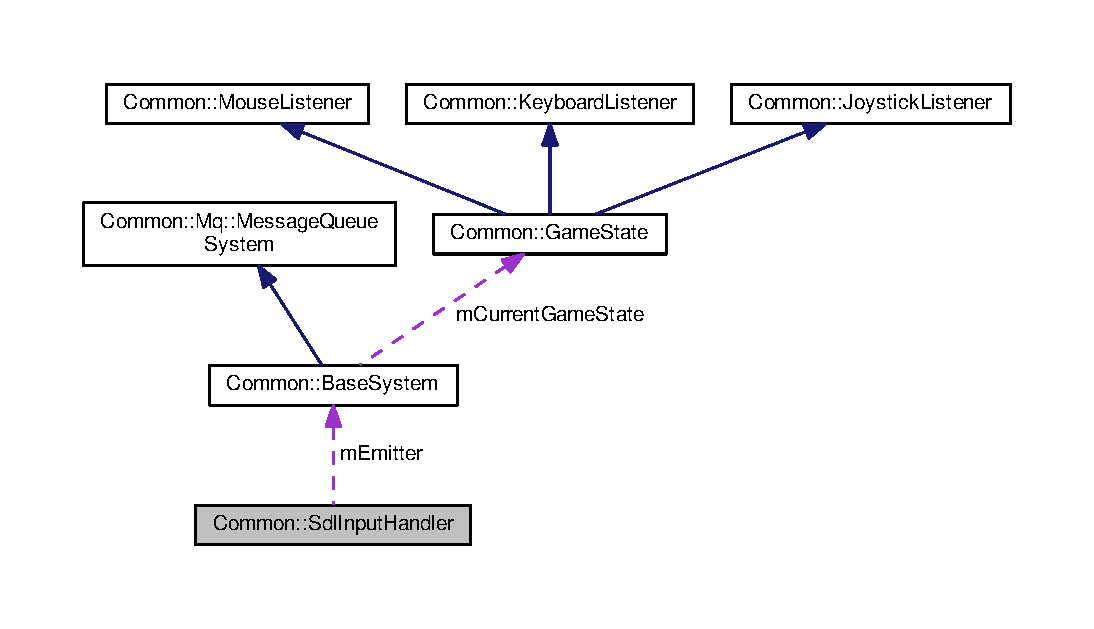
\includegraphics[width=350pt]{class_common_1_1_sdl_input_handler__coll__graph}
\end{center}
\end{figure}
\subsection*{Public Member Functions}
\begin{DoxyCompactItemize}
\item 
\hyperlink{class_common_1_1_sdl_input_handler_ac90801d445e5c31dcd2b965ca3eaef53}{Sdl\+Input\+Handler} (S\+D\+L\+\_\+\+Window $\ast$sdl\+Window, \hyperlink{class_common_1_1_base_system}{Base\+System} $\ast$emitter)
\item 
\mbox{\Hypertarget{class_common_1_1_sdl_input_handler_aee86cff741e688efe72e66e947592fed}\label{class_common_1_1_sdl_input_handler_aee86cff741e688efe72e66e947592fed}} 
virtual \hyperlink{class_common_1_1_sdl_input_handler_aee86cff741e688efe72e66e947592fed}{$\sim$\+Sdl\+Input\+Handler} ()
\begin{DoxyCompactList}\small\item\em Simple destructor. \end{DoxyCompactList}\item 
void \hyperlink{class_common_1_1_sdl_input_handler_a24ecda74ffbdad833809ec916ca5aa36}{\+\_\+handle\+Sdl\+Events} (const \hyperlink{union_s_d_l___event}{S\+D\+L\+\_\+\+Event} \&evt)
\item 
\mbox{\Hypertarget{class_common_1_1_sdl_input_handler_af59f3d8f841492da0d58d70a7194d18a}\label{class_common_1_1_sdl_input_handler_af59f3d8f841492da0d58d70a7194d18a}} 
void \hyperlink{class_common_1_1_sdl_input_handler_af59f3d8f841492da0d58d70a7194d18a}{set\+Grab\+Mouse\+Pointer} (bool grab)
\begin{DoxyCompactList}\small\item\em Locks the pointer to the window. \end{DoxyCompactList}\item 
void \hyperlink{class_common_1_1_sdl_input_handler_a93f3c75fde51291eb985afbc1877dfb7}{set\+Mouse\+Relative} (bool relative)
\item 
\mbox{\Hypertarget{class_common_1_1_sdl_input_handler_ac866cdab398f7fe1c2f77d186bb08d17}\label{class_common_1_1_sdl_input_handler_ac866cdab398f7fe1c2f77d186bb08d17}} 
void \hyperlink{class_common_1_1_sdl_input_handler_ac866cdab398f7fe1c2f77d186bb08d17}{set\+Mouse\+Visible} (bool visible)
\begin{DoxyCompactList}\small\item\em Show the cursor. \end{DoxyCompactList}\item 
void \hyperlink{class_common_1_1_sdl_input_handler_aa1a7c47e721048e1103db4038571f5c3}{add\+Receiver} (\hyperlink{class_common_1_1_base_system}{Base\+System} $\ast$receiver)
\item 
\mbox{\Hypertarget{class_common_1_1_sdl_input_handler_ac906f60b05f1593089322cfdaeab72b3}\label{class_common_1_1_sdl_input_handler_ac906f60b05f1593089322cfdaeab72b3}} 
void {\bfseries emit} (const \hyperlink{union_s_d_l___event}{S\+D\+L\+\_\+\+Event} \&evt)
\end{DoxyCompactItemize}
\subsection*{Private Member Functions}
\begin{DoxyCompactItemize}
\item 
\mbox{\Hypertarget{class_common_1_1_sdl_input_handler_a6fca1b5e89e3d0a250b220044b320d47}\label{class_common_1_1_sdl_input_handler_a6fca1b5e89e3d0a250b220044b320d47}} 
void \hyperlink{class_common_1_1_sdl_input_handler_a6fca1b5e89e3d0a250b220044b320d47}{update\+Mouse\+Settings} (void)
\begin{DoxyCompactList}\small\item\em Update mouse settings. \end{DoxyCompactList}\item 
\mbox{\Hypertarget{class_common_1_1_sdl_input_handler_aa47a9305fe7810fdff8c750123cf8e93}\label{class_common_1_1_sdl_input_handler_aa47a9305fe7810fdff8c750123cf8e93}} 
void \hyperlink{class_common_1_1_sdl_input_handler_aa47a9305fe7810fdff8c750123cf8e93}{handle\+Window\+Event} (const \hyperlink{union_s_d_l___event}{S\+D\+L\+\_\+\+Event} \&evt)
\begin{DoxyCompactList}\small\item\em Manage window event. \end{DoxyCompactList}\item 
void \hyperlink{class_common_1_1_sdl_input_handler_a589923be034191404d6597dfc8cee282}{warp\+Mouse} (int x, int y)
\item 
void \hyperlink{class_common_1_1_sdl_input_handler_aa73cf0ac43983be445f0fcf11e91eeef}{wrap\+Mouse\+Pointer} (const \hyperlink{struct_s_d_l___mouse_motion_event}{S\+D\+L\+\_\+\+Mouse\+Motion\+Event} \&evt)
\item 
bool \hyperlink{class_common_1_1_sdl_input_handler_a6ff9bcb5862bc2c14a13bbd573d6fdf4}{handle\+Warp\+Motion} (const \hyperlink{struct_s_d_l___mouse_motion_event}{S\+D\+L\+\_\+\+Mouse\+Motion\+Event} \&evt)
\end{DoxyCompactItemize}
\subsection*{Private Attributes}
\begin{DoxyCompactItemize}
\item 
\mbox{\Hypertarget{class_common_1_1_sdl_input_handler_a75f371e1643d00fd43a6fb8c6f8bae27}\label{class_common_1_1_sdl_input_handler_a75f371e1643d00fd43a6fb8c6f8bae27}} 
S\+D\+L\+\_\+\+Window $\ast$ \hyperlink{class_common_1_1_sdl_input_handler_a75f371e1643d00fd43a6fb8c6f8bae27}{m\+Sdl\+Window}
\begin{DoxyCompactList}\small\item\em Window of the program. \end{DoxyCompactList}\item 
\mbox{\Hypertarget{class_common_1_1_sdl_input_handler_a1b8a4b9d360bfe89087e00f3b7ae7fff}\label{class_common_1_1_sdl_input_handler_a1b8a4b9d360bfe89087e00f3b7ae7fff}} 
\hyperlink{class_common_1_1_base_system}{Base\+System} $\ast$ \hyperlink{class_common_1_1_sdl_input_handler_a1b8a4b9d360bfe89087e00f3b7ae7fff}{m\+Emitter}
\begin{DoxyCompactList}\small\item\em Emitter of the events. \end{DoxyCompactList}\item 
\mbox{\Hypertarget{class_common_1_1_sdl_input_handler_ad4debf0c68c6187b7fddcec3af1a0913}\label{class_common_1_1_sdl_input_handler_ad4debf0c68c6187b7fddcec3af1a0913}} 
std\+::vector$<$ \hyperlink{class_common_1_1_base_system}{Base\+System} $\ast$ $>$ \hyperlink{class_common_1_1_sdl_input_handler_ad4debf0c68c6187b7fddcec3af1a0913}{m\+Receivers}
\begin{DoxyCompactList}\small\item\em Receivers of the events. \end{DoxyCompactList}\item 
\mbox{\Hypertarget{class_common_1_1_sdl_input_handler_a821df0693764a084ec20b1087b796897}\label{class_common_1_1_sdl_input_handler_a821df0693764a084ec20b1087b796897}} 
bool \hyperlink{class_common_1_1_sdl_input_handler_a821df0693764a084ec20b1087b796897}{m\+Want\+Relative}
\begin{DoxyCompactList}\small\item\em User setting, whether the user wants the mouse to be relative or not. \end{DoxyCompactList}\item 
\mbox{\Hypertarget{class_common_1_1_sdl_input_handler_a97824bb249c9debfd331171ad3d27c01}\label{class_common_1_1_sdl_input_handler_a97824bb249c9debfd331171ad3d27c01}} 
bool \hyperlink{class_common_1_1_sdl_input_handler_a97824bb249c9debfd331171ad3d27c01}{m\+Want\+Mouse\+Grab}
\begin{DoxyCompactList}\small\item\em User setting, whether the user wants the mouse to be locked or not. \end{DoxyCompactList}\item 
\mbox{\Hypertarget{class_common_1_1_sdl_input_handler_a81ef820ecd55818d7ae9ff59edd1a5c1}\label{class_common_1_1_sdl_input_handler_a81ef820ecd55818d7ae9ff59edd1a5c1}} 
bool \hyperlink{class_common_1_1_sdl_input_handler_a81ef820ecd55818d7ae9ff59edd1a5c1}{m\+Want\+Mouse\+Visible}
\begin{DoxyCompactList}\small\item\em User setting, whether the user wants the mouse to be visible or not. \end{DoxyCompactList}\item 
\mbox{\Hypertarget{class_common_1_1_sdl_input_handler_ab94a01e84010e763d1bb1cabf999faad}\label{class_common_1_1_sdl_input_handler_ab94a01e84010e763d1bb1cabf999faad}} 
bool \hyperlink{class_common_1_1_sdl_input_handler_ab94a01e84010e763d1bb1cabf999faad}{m\+Is\+Mouse\+Relative}
\begin{DoxyCompactList}\small\item\em Whether the mouse is relative. \end{DoxyCompactList}\item 
\mbox{\Hypertarget{class_common_1_1_sdl_input_handler_a11822c2b4a5d7b2b09124b7b86baed4f}\label{class_common_1_1_sdl_input_handler_a11822c2b4a5d7b2b09124b7b86baed4f}} 
bool \hyperlink{class_common_1_1_sdl_input_handler_a11822c2b4a5d7b2b09124b7b86baed4f}{m\+Wrap\+Pointer\+Manually}
\begin{DoxyCompactList}\small\item\em Used when driver doesn\textquotesingle{}t support relative mode. \end{DoxyCompactList}\item 
\mbox{\Hypertarget{class_common_1_1_sdl_input_handler_a44b7f460f026184e21a0889a7724bd82}\label{class_common_1_1_sdl_input_handler_a44b7f460f026184e21a0889a7724bd82}} 
bool \hyperlink{class_common_1_1_sdl_input_handler_a44b7f460f026184e21a0889a7724bd82}{m\+Grab\+Pointer}
\begin{DoxyCompactList}\small\item\em Whether the pointer is lock. \end{DoxyCompactList}\item 
\mbox{\Hypertarget{class_common_1_1_sdl_input_handler_a45e3ba8c78c4f6a34c2012cdced052dc}\label{class_common_1_1_sdl_input_handler_a45e3ba8c78c4f6a34c2012cdced052dc}} 
bool \hyperlink{class_common_1_1_sdl_input_handler_a45e3ba8c78c4f6a34c2012cdced052dc}{m\+Mouse\+In\+Window}
\begin{DoxyCompactList}\small\item\em Whether the mouse is in the window. \end{DoxyCompactList}\item 
\mbox{\Hypertarget{class_common_1_1_sdl_input_handler_a30484ff0a8d8814168310570d7016504}\label{class_common_1_1_sdl_input_handler_a30484ff0a8d8814168310570d7016504}} 
bool \hyperlink{class_common_1_1_sdl_input_handler_a30484ff0a8d8814168310570d7016504}{m\+Window\+Has\+Focus}
\begin{DoxyCompactList}\small\item\em Whether the window has the focus. \end{DoxyCompactList}\item 
\mbox{\Hypertarget{class_common_1_1_sdl_input_handler_ac6b3b63d6b15aa1222e8e3ecf61e28ce}\label{class_common_1_1_sdl_input_handler_ac6b3b63d6b15aa1222e8e3ecf61e28ce}} 
Uint16 \hyperlink{class_common_1_1_sdl_input_handler_ac6b3b63d6b15aa1222e8e3ecf61e28ce}{m\+WarpX}
\begin{DoxyCompactList}\small\item\em X coordinate of the mouse. \end{DoxyCompactList}\item 
\mbox{\Hypertarget{class_common_1_1_sdl_input_handler_a2c2465331cf8e7a4b513859d8c6e756e}\label{class_common_1_1_sdl_input_handler_a2c2465331cf8e7a4b513859d8c6e756e}} 
Uint16 \hyperlink{class_common_1_1_sdl_input_handler_a2c2465331cf8e7a4b513859d8c6e756e}{m\+WarpY}
\begin{DoxyCompactList}\small\item\em Y coordinate of the mouse. \end{DoxyCompactList}\item 
\mbox{\Hypertarget{class_common_1_1_sdl_input_handler_a01bc2f782750bb5109a66d7f248f7c5c}\label{class_common_1_1_sdl_input_handler_a01bc2f782750bb5109a66d7f248f7c5c}} 
bool \hyperlink{class_common_1_1_sdl_input_handler_a01bc2f782750bb5109a66d7f248f7c5c}{m\+Warp\+Compensate}
\begin{DoxyCompactList}\small\item\em Whether the mouse has to be wrapped. \end{DoxyCompactList}\end{DoxyCompactItemize}


\subsection{Detailed Description}


Definition at line 18 of file Sdl\+Input\+Handler.\+h.



\subsection{Constructor \& Destructor Documentation}
\mbox{\Hypertarget{class_common_1_1_sdl_input_handler_ac90801d445e5c31dcd2b965ca3eaef53}\label{class_common_1_1_sdl_input_handler_ac90801d445e5c31dcd2b965ca3eaef53}} 
\index{Common\+::\+Sdl\+Input\+Handler@{Common\+::\+Sdl\+Input\+Handler}!Sdl\+Input\+Handler@{Sdl\+Input\+Handler}}
\index{Sdl\+Input\+Handler@{Sdl\+Input\+Handler}!Common\+::\+Sdl\+Input\+Handler@{Common\+::\+Sdl\+Input\+Handler}}
\subsubsection{\texorpdfstring{Sdl\+Input\+Handler()}{SdlInputHandler()}}
{\footnotesize\ttfamily Common\+::\+Sdl\+Input\+Handler\+::\+Sdl\+Input\+Handler (\begin{DoxyParamCaption}\item[{S\+D\+L\+\_\+\+Window $\ast$}]{sdl\+Window,  }\item[{\hyperlink{class_common_1_1_base_system}{Base\+System} $\ast$}]{emitter }\end{DoxyParamCaption})}

Constructor 
\begin{DoxyParams}{Parameters}
{\em sdl\+Window} & S\+D\+L\+\_\+\+Window receiving \hyperlink{union_s_d_l___event}{S\+D\+L\+\_\+\+Event} \\
\hline
{\em emitter} & \hyperlink{class_common_1_1_base_system}{Base\+System} which will send the events \\
\hline
\end{DoxyParams}


Definition at line 14 of file Sdl\+Input\+Handler.\+cpp.



\subsection{Member Function Documentation}
\mbox{\Hypertarget{class_common_1_1_sdl_input_handler_a24ecda74ffbdad833809ec916ca5aa36}\label{class_common_1_1_sdl_input_handler_a24ecda74ffbdad833809ec916ca5aa36}} 
\index{Common\+::\+Sdl\+Input\+Handler@{Common\+::\+Sdl\+Input\+Handler}!\+\_\+handle\+Sdl\+Events@{\+\_\+handle\+Sdl\+Events}}
\index{\+\_\+handle\+Sdl\+Events@{\+\_\+handle\+Sdl\+Events}!Common\+::\+Sdl\+Input\+Handler@{Common\+::\+Sdl\+Input\+Handler}}
\subsubsection{\texorpdfstring{\+\_\+handle\+Sdl\+Events()}{\_handleSdlEvents()}}
{\footnotesize\ttfamily void Common\+::\+Sdl\+Input\+Handler\+::\+\_\+handle\+Sdl\+Events (\begin{DoxyParamCaption}\item[{const \hyperlink{union_s_d_l___event}{S\+D\+L\+\_\+\+Event} \&}]{evt }\end{DoxyParamCaption})}

Decide what to do with events 
\begin{DoxyParams}{Parameters}
{\em evt} & \hyperlink{union_s_d_l___event}{S\+D\+L\+\_\+\+Event} to handle \\
\hline
\end{DoxyParams}


Definition at line 53 of file Sdl\+Input\+Handler.\+cpp.

\mbox{\Hypertarget{class_common_1_1_sdl_input_handler_aa1a7c47e721048e1103db4038571f5c3}\label{class_common_1_1_sdl_input_handler_aa1a7c47e721048e1103db4038571f5c3}} 
\index{Common\+::\+Sdl\+Input\+Handler@{Common\+::\+Sdl\+Input\+Handler}!add\+Receiver@{add\+Receiver}}
\index{add\+Receiver@{add\+Receiver}!Common\+::\+Sdl\+Input\+Handler@{Common\+::\+Sdl\+Input\+Handler}}
\subsubsection{\texorpdfstring{add\+Receiver()}{addReceiver()}}
{\footnotesize\ttfamily void Common\+::\+Sdl\+Input\+Handler\+::add\+Receiver (\begin{DoxyParamCaption}\item[{\hyperlink{class_common_1_1_base_system}{Base\+System} $\ast$}]{receiver }\end{DoxyParamCaption})}

Add a new receiver 
\begin{DoxyParams}{Parameters}
{\em receiver} & The new receiver \\
\hline
\end{DoxyParams}


Definition at line 155 of file Sdl\+Input\+Handler.\+cpp.

\mbox{\Hypertarget{class_common_1_1_sdl_input_handler_a6ff9bcb5862bc2c14a13bbd573d6fdf4}\label{class_common_1_1_sdl_input_handler_a6ff9bcb5862bc2c14a13bbd573d6fdf4}} 
\index{Common\+::\+Sdl\+Input\+Handler@{Common\+::\+Sdl\+Input\+Handler}!handle\+Warp\+Motion@{handle\+Warp\+Motion}}
\index{handle\+Warp\+Motion@{handle\+Warp\+Motion}!Common\+::\+Sdl\+Input\+Handler@{Common\+::\+Sdl\+Input\+Handler}}
\subsubsection{\texorpdfstring{handle\+Warp\+Motion()}{handleWarpMotion()}}
{\footnotesize\ttfamily bool Common\+::\+Sdl\+Input\+Handler\+::handle\+Warp\+Motion (\begin{DoxyParamCaption}\item[{const \hyperlink{struct_s_d_l___mouse_motion_event}{S\+D\+L\+\_\+\+Mouse\+Motion\+Event} \&}]{evt }\end{DoxyParamCaption})\hspace{0.3cm}{\ttfamily [private]}}

Internal method for ignoring relative motions as a side effect of \hyperlink{class_common_1_1_sdl_input_handler_a589923be034191404d6597dfc8cee282}{warp\+Mouse()} 
\begin{DoxyParams}{Parameters}
{\em evt} & Event containing mouse data \\
\hline
\end{DoxyParams}


Definition at line 143 of file Sdl\+Input\+Handler.\+cpp.

\mbox{\Hypertarget{class_common_1_1_sdl_input_handler_a93f3c75fde51291eb985afbc1877dfb7}\label{class_common_1_1_sdl_input_handler_a93f3c75fde51291eb985afbc1877dfb7}} 
\index{Common\+::\+Sdl\+Input\+Handler@{Common\+::\+Sdl\+Input\+Handler}!set\+Mouse\+Relative@{set\+Mouse\+Relative}}
\index{set\+Mouse\+Relative@{set\+Mouse\+Relative}!Common\+::\+Sdl\+Input\+Handler@{Common\+::\+Sdl\+Input\+Handler}}
\subsubsection{\texorpdfstring{set\+Mouse\+Relative()}{setMouseRelative()}}
{\footnotesize\ttfamily void Common\+::\+Sdl\+Input\+Handler\+::set\+Mouse\+Relative (\begin{DoxyParamCaption}\item[{bool}]{relative }\end{DoxyParamCaption})}

Set the mouse to relative positioning mode (when not supported by hardware, we emulate the behavior). From the S\+DL docs\+: While the mouse is in relative mode, the cursor is hidden, and the driver will try to report continuous motion in the current window. Only relative motion events will be delivered, the mouse position will not change 

Definition at line 87 of file Sdl\+Input\+Handler.\+cpp.

\mbox{\Hypertarget{class_common_1_1_sdl_input_handler_a589923be034191404d6597dfc8cee282}\label{class_common_1_1_sdl_input_handler_a589923be034191404d6597dfc8cee282}} 
\index{Common\+::\+Sdl\+Input\+Handler@{Common\+::\+Sdl\+Input\+Handler}!warp\+Mouse@{warp\+Mouse}}
\index{warp\+Mouse@{warp\+Mouse}!Common\+::\+Sdl\+Input\+Handler@{Common\+::\+Sdl\+Input\+Handler}}
\subsubsection{\texorpdfstring{warp\+Mouse()}{warpMouse()}}
{\footnotesize\ttfamily void Common\+::\+Sdl\+Input\+Handler\+::warp\+Mouse (\begin{DoxyParamCaption}\item[{int}]{x,  }\item[{int}]{y }\end{DoxyParamCaption})\hspace{0.3cm}{\ttfamily [private]}}

Moves the mouse to the specified point within the viewport 
\begin{DoxyParams}{Parameters}
{\em x} & X coordinate \\
\hline
{\em y} & Y coordinate \\
\hline
\end{DoxyParams}


Definition at line 119 of file Sdl\+Input\+Handler.\+cpp.

\mbox{\Hypertarget{class_common_1_1_sdl_input_handler_aa73cf0ac43983be445f0fcf11e91eeef}\label{class_common_1_1_sdl_input_handler_aa73cf0ac43983be445f0fcf11e91eeef}} 
\index{Common\+::\+Sdl\+Input\+Handler@{Common\+::\+Sdl\+Input\+Handler}!wrap\+Mouse\+Pointer@{wrap\+Mouse\+Pointer}}
\index{wrap\+Mouse\+Pointer@{wrap\+Mouse\+Pointer}!Common\+::\+Sdl\+Input\+Handler@{Common\+::\+Sdl\+Input\+Handler}}
\subsubsection{\texorpdfstring{wrap\+Mouse\+Pointer()}{wrapMousePointer()}}
{\footnotesize\ttfamily void Common\+::\+Sdl\+Input\+Handler\+::wrap\+Mouse\+Pointer (\begin{DoxyParamCaption}\item[{const \hyperlink{struct_s_d_l___mouse_motion_event}{S\+D\+L\+\_\+\+Mouse\+Motion\+Event} \&}]{evt }\end{DoxyParamCaption})\hspace{0.3cm}{\ttfamily [private]}}

Prevents the mouse cursor from leaving the window 
\begin{DoxyParams}{Parameters}
{\em evt} & Event containing mouse data \\
\hline
\end{DoxyParams}


Definition at line 126 of file Sdl\+Input\+Handler.\+cpp.



The documentation for this class was generated from the following files\+:\begin{DoxyCompactItemize}
\item 
/home/louis/projects/\+Le\+Dernier\+Morkid/\+Common/include/Sdl\+Input\+Handler.\+h\item 
/home/louis/projects/\+Le\+Dernier\+Morkid/\+Common/src/Sdl\+Input\+Handler.\+cpp\end{DoxyCompactItemize}

\hypertarget{class_shadow_mapper}{}\section{Shadow\+Mapper Class Reference}
\label{class_shadow_mapper}\index{Shadow\+Mapper@{Shadow\+Mapper}}
\subsection*{Public Member Functions}
\begin{DoxyCompactItemize}
\item 
\mbox{\Hypertarget{class_shadow_mapper_a83504b2db6dc914c993011d388d3c139}\label{class_shadow_mapper_a83504b2db6dc914c993011d388d3c139}} 
{\bfseries Shadow\+Mapper} (Ogre\+::\+Scene\+Manager $\ast$scene\+Manager, Ogre\+::\+Compositor\+Manager2 $\ast$compositor\+Manager)
\item 
void \hyperlink{class_shadow_mapper_a5438f906adc558347171a1d4fbbe616d}{set\+Gaussian\+Filter\+Params} (Ogre\+::uint8 kernel\+Radius, float gaussian\+Deviation\+Factor=0.\+5f)
\item 
\mbox{\Hypertarget{class_shadow_mapper_a05511961c2261cd32eacf534bf0873a8}\label{class_shadow_mapper_a05511961c2261cd32eacf534bf0873a8}} 
void {\bfseries create\+Shadow\+Map} (Ogre\+::\+Id\+Type id, Ogre\+::\+Texture\+Ptr \&height\+Map\+Tex)
\item 
\mbox{\Hypertarget{class_shadow_mapper_aaa7a869e868690bf241b83d9bcb8626d}\label{class_shadow_mapper_aaa7a869e868690bf241b83d9bcb8626d}} 
void {\bfseries destroy\+Shadow\+Map} (void)
\item 
\mbox{\Hypertarget{class_shadow_mapper_afa29619eed1b51a4088bbfbd64cf1a1a}\label{class_shadow_mapper_afa29619eed1b51a4088bbfbd64cf1a1a}} 
void {\bfseries update\+Shadow\+Map} (const Ogre\+::\+Vector3 \&light\+Dir, const Ogre\+::\+Vector2 \&xz\+Dimensions, float height\+Scale)
\item 
\mbox{\Hypertarget{class_shadow_mapper_a993ea2a8424fc5b966bac231b14c5353}\label{class_shadow_mapper_a993ea2a8424fc5b966bac231b14c5353}} 
void {\bfseries fill\+Uav\+Data\+For\+Compositor\+Channel} (Ogre\+::\+Compositor\+Channel \&out\+Channel, Ogre\+::\+Resource\+Layout\+Map \&out\+Initial\+Layouts, Ogre\+::\+Resource\+Access\+Map \&out\+Initial\+Uav\+Access) const
\item 
\mbox{\Hypertarget{class_shadow_mapper_a624f59c26a8831b0e3bbabb82ef9a822}\label{class_shadow_mapper_a624f59c26a8831b0e3bbabb82ef9a822}} 
Ogre\+::\+Texture\+Ptr {\bfseries get\+Shadow\+Map\+Tex} (void) const
\end{DoxyCompactItemize}
\subsection*{Static Private Member Functions}
\begin{DoxyCompactItemize}
\item 
\mbox{\Hypertarget{class_shadow_mapper_a54d854ea5525ec6cffaf5958d1d4077a}\label{class_shadow_mapper_a54d854ea5525ec6cffaf5958d1d4077a}} 
static size\+\_\+t {\bfseries get\+Starts\+Ptr\+Count} (Ogre\+::int32 $\ast$starts, Ogre\+::int32 $\ast$starts\+Base)
\item 
static Ogre\+::int32 \hyperlink{class_shadow_mapper_a35a0aa58c648464248c2a9060f522921}{get\+X\+Steps\+Needed\+To\+ReachY} (Ogre\+::uint32 y, float f\+Step)
\item 
static float \hyperlink{class_shadow_mapper_ae95d31a0216503b8838738e959e32b1c}{get\+Error\+After\+Xsteps} (Ogre\+::uint32 x\+Iterations\+To\+Skip, float dx, float dy)
\item 
\mbox{\Hypertarget{class_shadow_mapper_a1b07d0963a08cede75e24c8a99c5f52f}\label{class_shadow_mapper_a1b07d0963a08cede75e24c8a99c5f52f}} 
static void {\bfseries set\+Gaussian\+Filter\+Params} (Ogre\+::\+Hlms\+Compute\+Job $\ast$job, Ogre\+::uint8 kernel\+Radius, float gaussian\+Deviation\+Factor=0.\+5f)
\end{DoxyCompactItemize}
\subsection*{Private Attributes}
\begin{DoxyCompactItemize}
\item 
\mbox{\Hypertarget{class_shadow_mapper_ae776a60c15e939d1f410e2c76f11c36b}\label{class_shadow_mapper_ae776a60c15e939d1f410e2c76f11c36b}} 
Ogre\+::\+Texture\+Ptr {\bfseries m\+Height\+Map\+Tex}
\item 
\mbox{\Hypertarget{class_shadow_mapper_a25a59b36221761ff585466bd007b57b6}\label{class_shadow_mapper_a25a59b36221761ff585466bd007b57b6}} 
Ogre\+::\+Const\+Buffer\+Packed $\ast$ {\bfseries m\+Shadow\+Starts}
\item 
\mbox{\Hypertarget{class_shadow_mapper_aadb1c723556b6bd7f820367a61def60d}\label{class_shadow_mapper_aadb1c723556b6bd7f820367a61def60d}} 
Ogre\+::\+Const\+Buffer\+Packed $\ast$ {\bfseries m\+Shadow\+Per\+Group\+Data}
\item 
\mbox{\Hypertarget{class_shadow_mapper_af384525eff0397e825335cac1383035a}\label{class_shadow_mapper_af384525eff0397e825335cac1383035a}} 
Ogre\+::\+Compositor\+Workspace $\ast$ {\bfseries m\+Shadow\+Workspace}
\item 
\mbox{\Hypertarget{class_shadow_mapper_aa4ce21c6dc95445db1260e5c63a9b385}\label{class_shadow_mapper_aa4ce21c6dc95445db1260e5c63a9b385}} 
Ogre\+::\+Texture\+Ptr {\bfseries m\+Shadow\+Map\+Tex}
\item 
\mbox{\Hypertarget{class_shadow_mapper_a5c17b8b5ec20194c4fb4a7ff1de984f5}\label{class_shadow_mapper_a5c17b8b5ec20194c4fb4a7ff1de984f5}} 
Ogre\+::\+Hlms\+Compute\+Job $\ast$ {\bfseries m\+Shadow\+Job}
\item 
\mbox{\Hypertarget{class_shadow_mapper_a05350d603d5cfad35eda8743abc1ecac}\label{class_shadow_mapper_a05350d603d5cfad35eda8743abc1ecac}} 
Ogre\+::\+Shader\+Params\+::\+Param $\ast$ {\bfseries m\+Job\+Param\+Delta}
\item 
\mbox{\Hypertarget{class_shadow_mapper_aadeaa1e03b1336e1a7766cb0bbd6ce6d}\label{class_shadow_mapper_aadeaa1e03b1336e1a7766cb0bbd6ce6d}} 
Ogre\+::\+Shader\+Params\+::\+Param $\ast$ {\bfseries m\+Job\+Param\+X\+Y\+Step}
\item 
\mbox{\Hypertarget{class_shadow_mapper_ae71ddf6f440e83eaefe0c896fc5b2829}\label{class_shadow_mapper_ae71ddf6f440e83eaefe0c896fc5b2829}} 
Ogre\+::\+Shader\+Params\+::\+Param $\ast$ {\bfseries m\+Job\+Param\+Is\+Step}
\item 
\mbox{\Hypertarget{class_shadow_mapper_a51147036e095f3889d5529a61c83157e}\label{class_shadow_mapper_a51147036e095f3889d5529a61c83157e}} 
Ogre\+::\+Shader\+Params\+::\+Param $\ast$ {\bfseries m\+Job\+Param\+Height\+Delta}
\item 
\mbox{\Hypertarget{class_shadow_mapper_aceb39870c1d238da7f6c91001a6fa860}\label{class_shadow_mapper_aceb39870c1d238da7f6c91001a6fa860}} 
Ogre\+::\+Scene\+Manager $\ast$ {\bfseries m\+Scene\+Manager}
\item 
\mbox{\Hypertarget{class_shadow_mapper_afa176dac98a1f33e9b27b6bff4e8e8f0}\label{class_shadow_mapper_afa176dac98a1f33e9b27b6bff4e8e8f0}} 
Ogre\+::\+Compositor\+Manager2 $\ast$ {\bfseries m\+Compositor\+Manager}
\end{DoxyCompactItemize}


\subsection{Detailed Description}


Definition at line 14 of file Terrain\+Shadow\+Mapper.\+h.



\subsection{Member Function Documentation}
\mbox{\Hypertarget{class_shadow_mapper_ae95d31a0216503b8838738e959e32b1c}\label{class_shadow_mapper_ae95d31a0216503b8838738e959e32b1c}} 
\index{Shadow\+Mapper@{Shadow\+Mapper}!get\+Error\+After\+Xsteps@{get\+Error\+After\+Xsteps}}
\index{get\+Error\+After\+Xsteps@{get\+Error\+After\+Xsteps}!Shadow\+Mapper@{Shadow\+Mapper}}
\subsubsection{\texorpdfstring{get\+Error\+After\+Xsteps()}{getErrorAfterXsteps()}}
{\footnotesize\ttfamily float Shadow\+Mapper\+::get\+Error\+After\+Xsteps (\begin{DoxyParamCaption}\item[{Ogre\+::uint32}]{x\+Iterations\+To\+Skip,  }\item[{float}]{dx,  }\item[{float}]{dy }\end{DoxyParamCaption})\hspace{0.3cm}{\ttfamily [inline]}, {\ttfamily [static]}, {\ttfamily [private]}}

Calculates the value of the error at position x = x\+Iterations\+To\+Skip from Bresenham\textquotesingle{}s algorithm. \begin{DoxyRemark}{Remarks}
We use this function so we can start Bresenham from \textquotesingle{}0\textquotesingle{} but resuming as if we wouldn\textquotesingle{}t be starting from 0. 
\end{DoxyRemark}

\begin{DoxyParams}{Parameters}
{\em x\+Iterations\+To\+Skip} & The X position in which we want the error. \\
\hline
{\em dx} & delta.\+x \\
\hline
{\em dy} & delta.\+y \\
\hline
\end{DoxyParams}
\begin{DoxyReturn}{Returns}
The error at position (x\+Iterations\+To\+Skip; y) 
\end{DoxyReturn}


Definition at line 129 of file Terrain\+Shadow\+Mapper.\+cpp.

\mbox{\Hypertarget{class_shadow_mapper_a35a0aa58c648464248c2a9060f522921}\label{class_shadow_mapper_a35a0aa58c648464248c2a9060f522921}} 
\index{Shadow\+Mapper@{Shadow\+Mapper}!get\+X\+Steps\+Needed\+To\+ReachY@{get\+X\+Steps\+Needed\+To\+ReachY}}
\index{get\+X\+Steps\+Needed\+To\+ReachY@{get\+X\+Steps\+Needed\+To\+ReachY}!Shadow\+Mapper@{Shadow\+Mapper}}
\subsubsection{\texorpdfstring{get\+X\+Steps\+Needed\+To\+Reach\+Y()}{getXStepsNeededToReachY()}}
{\footnotesize\ttfamily Ogre\+::int32 Shadow\+Mapper\+::get\+X\+Steps\+Needed\+To\+ReachY (\begin{DoxyParamCaption}\item[{Ogre\+::uint32}]{y,  }\item[{float}]{f\+Step }\end{DoxyParamCaption})\hspace{0.3cm}{\ttfamily [inline]}, {\ttfamily [static]}, {\ttfamily [private]}}

Gets how many steps are needed in Bresenham\textquotesingle{}s algorithm to reach certain height, given its dx / dy ratio where\+: dx = abs( x1 -\/ x0 ); dy = abs( y1 -\/ y0 ); and Bresenham is drawn in ranges \mbox{[}x0; x1) and \mbox{[}y0; y1) 
\begin{DoxyParams}{Parameters}
{\em y} & Height to reach \\
\hline
{\em f\+Step} & (dx $\ast$ 0.\+5f) / dy; \\
\hline
\end{DoxyParams}
\begin{DoxyReturn}{Returns}
Number of X iterations needed to reach the the pixel at height \textquotesingle{}y\textquotesingle{} The returned value is at position (ret\+Val; y) which means (ret\+Val-\/1; y-\/1) is true unless y = 0; 
\end{DoxyReturn}


Definition at line 125 of file Terrain\+Shadow\+Mapper.\+cpp.

\mbox{\Hypertarget{class_shadow_mapper_a5438f906adc558347171a1d4fbbe616d}\label{class_shadow_mapper_a5438f906adc558347171a1d4fbbe616d}} 
\index{Shadow\+Mapper@{Shadow\+Mapper}!set\+Gaussian\+Filter\+Params@{set\+Gaussian\+Filter\+Params}}
\index{set\+Gaussian\+Filter\+Params@{set\+Gaussian\+Filter\+Params}!Shadow\+Mapper@{Shadow\+Mapper}}
\subsubsection{\texorpdfstring{set\+Gaussian\+Filter\+Params()}{setGaussianFilterParams()}}
{\footnotesize\ttfamily void Shadow\+Mapper\+::set\+Gaussian\+Filter\+Params (\begin{DoxyParamCaption}\item[{Ogre\+::uint8}]{kernel\+Radius,  }\item[{float}]{gaussian\+Deviation\+Factor = {\ttfamily 0.5f} }\end{DoxyParamCaption})}

Sets the parameter of the gaussian filter we apply to the shadow map. 
\begin{DoxyParams}{Parameters}
{\em kernel\+Radius} & Kernel radius. Must be an even number. \\
\hline
{\em gaussian\+Deviation\+Factor} & Expressed in terms of gaussian\+Deviation = kernel\+Radius $\ast$ gaussian\+Deviation\+Factor \\
\hline
\end{DoxyParams}


Definition at line 324 of file Terrain\+Shadow\+Mapper.\+cpp.



The documentation for this class was generated from the following files\+:\begin{DoxyCompactItemize}
\item 
/home/louis/projects/\+Le\+Dernier\+Morkid/include/\+Terrain/Terrain\+Shadow\+Mapper.\+h\item 
/home/louis/projects/\+Le\+Dernier\+Morkid/src/\+Terrain/Terrain\+Shadow\+Mapper.\+cpp\end{DoxyCompactItemize}

\hypertarget{class_common_1_1_static_plugin_loader}{}\section{Common\+:\+:Static\+Plugin\+Loader Class Reference}
\label{class_common_1_1_static_plugin_loader}\index{Common\+::\+Static\+Plugin\+Loader@{Common\+::\+Static\+Plugin\+Loader}}


Utility class to load plugins statically.  




{\ttfamily \#include $<$Static\+Plugin\+Loader.\+h$>$}

\subsection*{Public Member Functions}
\begin{DoxyCompactItemize}
\item 
\mbox{\Hypertarget{class_common_1_1_static_plugin_loader_a4d07878bdf153243742618252174fdb1}\label{class_common_1_1_static_plugin_loader_a4d07878bdf153243742618252174fdb1}} 
\hyperlink{class_common_1_1_static_plugin_loader_a4d07878bdf153243742618252174fdb1}{Static\+Plugin\+Loader} ()
\begin{DoxyCompactList}\small\item\em Simple Constructor. \end{DoxyCompactList}\item 
\mbox{\Hypertarget{class_common_1_1_static_plugin_loader_a664472b3a72a71fbe5be7653bcc29b38}\label{class_common_1_1_static_plugin_loader_a664472b3a72a71fbe5be7653bcc29b38}} 
\hyperlink{class_common_1_1_static_plugin_loader_a664472b3a72a71fbe5be7653bcc29b38}{$\sim$\+Static\+Plugin\+Loader} ()
\begin{DoxyCompactList}\small\item\em Simple Destructor. \end{DoxyCompactList}\item 
void \hyperlink{class_common_1_1_static_plugin_loader_ad53a802ca29d709d2e2731be6304d274}{install} (Ogre\+::\+Root $\ast$root)
\end{DoxyCompactItemize}


\subsection{Detailed Description}
Utility class to load plugins statically. 

\begin{DoxyRemark}{Remarks}
This class is only useful if you want to use the Metal Rendersystem 
\end{DoxyRemark}


Definition at line 56 of file Static\+Plugin\+Loader.\+h.



\subsection{Member Function Documentation}
\mbox{\Hypertarget{class_common_1_1_static_plugin_loader_ad53a802ca29d709d2e2731be6304d274}\label{class_common_1_1_static_plugin_loader_ad53a802ca29d709d2e2731be6304d274}} 
\index{Common\+::\+Static\+Plugin\+Loader@{Common\+::\+Static\+Plugin\+Loader}!install@{install}}
\index{install@{install}!Common\+::\+Static\+Plugin\+Loader@{Common\+::\+Static\+Plugin\+Loader}}
\subsubsection{\texorpdfstring{install()}{install()}}
{\footnotesize\ttfamily void Common\+::\+Static\+Plugin\+Loader\+::install (\begin{DoxyParamCaption}\item[{Ogre\+::\+Root $\ast$}]{root }\end{DoxyParamCaption})}

Method which install Metal plugin depending on your Ogre configuration 
\begin{DoxyParams}{Parameters}
{\em root} & The Ogre\+::\+Root who will install the plugin \\
\hline
\end{DoxyParams}


Definition at line 61 of file Static\+Plugin\+Loader.\+cpp.



The documentation for this class was generated from the following files\+:\begin{DoxyCompactItemize}
\item 
/home/louis/projects/\+Le\+Dernier\+Morkid/\+Common/include/\+System/Static\+Plugin\+Loader.\+h\item 
/home/louis/projects/\+Le\+Dernier\+Morkid/\+Common/src/\+System/Static\+Plugin\+Loader.\+cpp\end{DoxyCompactItemize}

\hypertarget{class_terrain}{}\section{Terrain Class Reference}
\label{class_terrain}\index{Terrain@{Terrain}}


Inheritance diagram for Terrain\+:\nopagebreak
\begin{figure}[H]
\begin{center}
\leavevmode
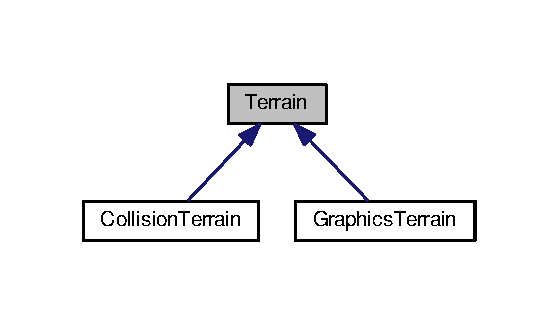
\includegraphics[width=268pt]{class_terrain__inherit__graph}
\end{center}
\end{figure}
\subsection*{Public Member Functions}
\begin{DoxyCompactItemize}
\item 
\mbox{\Hypertarget{class_terrain_a8f77d3aac1e178496309536f980c27fe}\label{class_terrain_a8f77d3aac1e178496309536f980c27fe}} 
virtual void {\bfseries load} (Ogre\+::\+Image \&image, const Ogre\+::\+Vector3 center, const Ogre\+::\+Vector3 \&dimensions)
\item 
\mbox{\Hypertarget{class_terrain_a02b19ca469ed94b895ceadfc526203c3}\label{class_terrain_a02b19ca469ed94b895ceadfc526203c3}} 
virtual bool {\bfseries get\+Height\+At} (Ogre\+::\+Vector3 \&v\+Pos) const
\item 
\mbox{\Hypertarget{class_terrain_a5802486dd915b658773e292f797fd72b}\label{class_terrain_a5802486dd915b658773e292f797fd72b}} 
virtual const Ogre\+::\+Vector2 \& {\bfseries get\+X\+Z\+Dimensions} (void) const
\item 
\mbox{\Hypertarget{class_terrain_a65bec8a0b02007377f8f7432645d9290}\label{class_terrain_a65bec8a0b02007377f8f7432645d9290}} 
virtual const Ogre\+::\+Vector2 \& {\bfseries get\+X\+Z\+Inv\+Dimensions} (void) const
\item 
\mbox{\Hypertarget{class_terrain_a9a99a3fd62c958faea6cc07f0e23e8d9}\label{class_terrain_a9a99a3fd62c958faea6cc07f0e23e8d9}} 
virtual float {\bfseries get\+Height} (void) const
\item 
\mbox{\Hypertarget{class_terrain_a22b6a113ff0f3bd7ff43b9d2fb201a68}\label{class_terrain_a22b6a113ff0f3bd7ff43b9d2fb201a68}} 
virtual const Ogre\+::\+Vector3 \& {\bfseries get\+Terrain\+Origin} (void) const
\end{DoxyCompactItemize}
\subsection*{Protected Member Functions}
\begin{DoxyCompactItemize}
\item 
\mbox{\Hypertarget{class_terrain_a54f91ef044931634522b62bdcb692e3f}\label{class_terrain_a54f91ef044931634522b62bdcb692e3f}} 
virtual Ogre\+::\+Image {\bfseries load\+Image} (const Ogre\+::\+String \&image\+Name)
\item 
\mbox{\Hypertarget{class_terrain_aac07c957e4dda6deaca7c1924f58cb99}\label{class_terrain_aac07c957e4dda6deaca7c1924f58cb99}} 
virtual void {\bfseries create\+Heightmap} (Ogre\+::\+Image \&image)
\item 
\mbox{\Hypertarget{class_terrain_a36055197e9913fba0b3a6ef7ed35a01d}\label{class_terrain_a36055197e9913fba0b3a6ef7ed35a01d}} 
void {\bfseries create\+Heightmap\+Texture} (const Ogre\+::\+String \&image\+Name, const Ogre\+::\+Image \&image)
\item 
\mbox{\Hypertarget{class_terrain_a30772767fde11e818ff80a0d60be2283}\label{class_terrain_a30772767fde11e818ff80a0d60be2283}} 
void {\bfseries destroy\+Heightmap\+Texture} (void)
\item 
\mbox{\Hypertarget{class_terrain_af53bde3d676e2627132f65e70527f900}\label{class_terrain_af53bde3d676e2627132f65e70527f900}} 
virtual \hyperlink{struct_grid_point}{Grid\+Point} {\bfseries world\+To\+Grid} (const Ogre\+::\+Vector3 \&v\+Pos) const
\item 
\mbox{\Hypertarget{class_terrain_a3ded300819839623b59f9d4c8809b8cd}\label{class_terrain_a3ded300819839623b59f9d4c8809b8cd}} 
virtual Ogre\+::\+Vector2 {\bfseries grid\+To\+World} (const \hyperlink{struct_grid_point}{Grid\+Point} \&g\+Pos) const
\item 
\mbox{\Hypertarget{class_terrain_a1446e1ac3b4d31613fdb82b38c6e055f}\label{class_terrain_a1446e1ac3b4d31613fdb82b38c6e055f}} 
virtual void {\bfseries calculate\+Optimum\+Skirt\+Size} (void)
\end{DoxyCompactItemize}
\subsection*{Protected Attributes}
\begin{DoxyCompactItemize}
\item 
\mbox{\Hypertarget{class_terrain_a0e7124f6a957a2adabe4820f9f96609d}\label{class_terrain_a0e7124f6a957a2adabe4820f9f96609d}} 
std\+::vector$<$ float $>$ {\bfseries m\+Height\+Map}
\item 
\mbox{\Hypertarget{class_terrain_a6ea67033a348cbe2c2f1a30130ee9fa2}\label{class_terrain_a6ea67033a348cbe2c2f1a30130ee9fa2}} 
Ogre\+::uint32 {\bfseries m\+Width}
\item 
\mbox{\Hypertarget{class_terrain_a0c09ca663727370da6c32e700260c97d}\label{class_terrain_a0c09ca663727370da6c32e700260c97d}} 
Ogre\+::uint32 {\bfseries m\+Depth}
\item 
\mbox{\Hypertarget{class_terrain_a069c3ccaa388a69a0234cd439613f227}\label{class_terrain_a069c3ccaa388a69a0234cd439613f227}} 
float {\bfseries m\+Depth\+Width\+Ratio}
\item 
\mbox{\Hypertarget{class_terrain_a954d59e15e7015f7d35dfd540eec5614}\label{class_terrain_a954d59e15e7015f7d35dfd540eec5614}} 
float {\bfseries m\+Skirt\+Size}
\item 
\mbox{\Hypertarget{class_terrain_a3c2af35db2a535399da1042dfaa33f7a}\label{class_terrain_a3c2af35db2a535399da1042dfaa33f7a}} 
float {\bfseries m\+Inv\+Width}
\item 
\mbox{\Hypertarget{class_terrain_a7a558b8126aa9cbe1db94d8594c23b10}\label{class_terrain_a7a558b8126aa9cbe1db94d8594c23b10}} 
float {\bfseries m\+Inv\+Depth}
\item 
\mbox{\Hypertarget{class_terrain_a51ed9c18ce43049069d91050725b02f6}\label{class_terrain_a51ed9c18ce43049069d91050725b02f6}} 
Ogre\+::uint32 {\bfseries m\+Base\+Pixel\+Dimension}
\item 
\mbox{\Hypertarget{class_terrain_aa69fad98c484b1693e6799dd43b63740}\label{class_terrain_aa69fad98c484b1693e6799dd43b63740}} 
Ogre\+::\+Vector2 {\bfseries m\+X\+Z\+Dimensions}
\item 
\mbox{\Hypertarget{class_terrain_a259c829335b24569bd1a4b14f8a0112f}\label{class_terrain_a259c829335b24569bd1a4b14f8a0112f}} 
Ogre\+::\+Vector2 {\bfseries m\+X\+Z\+Inv\+Dimensions}
\item 
\mbox{\Hypertarget{class_terrain_a957653a8d23d3655c025765914f54fbf}\label{class_terrain_a957653a8d23d3655c025765914f54fbf}} 
Ogre\+::\+Vector2 {\bfseries m\+X\+Z\+Relative\+Size}
\item 
\mbox{\Hypertarget{class_terrain_afb0c042f174d26d388fa4ccbcf5e7b35}\label{class_terrain_afb0c042f174d26d388fa4ccbcf5e7b35}} 
float {\bfseries m\+Height}
\item 
\mbox{\Hypertarget{class_terrain_a96a43b46173a00ed494f4e33e479692e}\label{class_terrain_a96a43b46173a00ed494f4e33e479692e}} 
Ogre\+::\+Vector3 {\bfseries m\+Terrain\+Origin}
\item 
\mbox{\Hypertarget{class_terrain_a2531cf9b13520ac5a59d03850057ec30}\label{class_terrain_a2531cf9b13520ac5a59d03850057ec30}} 
Ogre\+::\+Texture\+Ptr {\bfseries m\+Height\+Map\+Tex}
\end{DoxyCompactItemize}
\subsection*{Friends}
\begin{DoxyCompactItemize}
\item 
\mbox{\Hypertarget{class_terrain_a403e723a938a88a4e53eb87b478db7c0}\label{class_terrain_a403e723a938a88a4e53eb87b478db7c0}} 
class {\bfseries Terrain\+Cell}
\end{DoxyCompactItemize}


The documentation for this class was generated from the following files\+:\begin{DoxyCompactItemize}
\item 
/home/louis/projects/\+Le\+Dernier\+Morkid/include/\+Terrain/Terrain.\+h\item 
/home/louis/projects/\+Le\+Dernier\+Morkid/src/\+Terrain/Terrain.\+cpp\end{DoxyCompactItemize}

\hypertarget{struct_terrain_baked_texture}{}\section{Terrain\+Baked\+Texture Struct Reference}
\label{struct_terrain_baked_texture}\index{Terrain\+Baked\+Texture@{Terrain\+Baked\+Texture}}
\subsection*{Public Member Functions}
\begin{DoxyCompactItemize}
\item 
\mbox{\Hypertarget{struct_terrain_baked_texture_a662c33c58c79a184be57c48cff7ebdff}\label{struct_terrain_baked_texture_a662c33c58c79a184be57c48cff7ebdff}} 
{\bfseries Terrain\+Baked\+Texture} (const Ogre\+::\+Texture\+Ptr tex, const Ogre\+::\+Hlms\+Samplerblock $\ast$\+\_\+sampler\+Block)
\item 
\mbox{\Hypertarget{struct_terrain_baked_texture_a7654b92aa3209e29c6b04b89d7134945}\label{struct_terrain_baked_texture_a7654b92aa3209e29c6b04b89d7134945}} 
bool {\bfseries operator==} (const \hyperlink{struct_terrain_baked_texture}{Terrain\+Baked\+Texture} \&\+\_\+r) const
\end{DoxyCompactItemize}
\subsection*{Public Attributes}
\begin{DoxyCompactItemize}
\item 
\mbox{\Hypertarget{struct_terrain_baked_texture_aee3e546c44ff51c6954a3433b453747c}\label{struct_terrain_baked_texture_aee3e546c44ff51c6954a3433b453747c}} 
Ogre\+::\+Texture\+Ptr {\bfseries texture}
\item 
\mbox{\Hypertarget{struct_terrain_baked_texture_af238f5927b36e48a6066fe597acf90a8}\label{struct_terrain_baked_texture_af238f5927b36e48a6066fe597acf90a8}} 
Ogre\+::\+Hlms\+Samplerblock const  $\ast$ {\bfseries sampler\+Block}
\end{DoxyCompactItemize}


The documentation for this struct was generated from the following file\+:\begin{DoxyCompactItemize}
\item 
/home/louis/projects/\+Le\+Dernier\+Morkid/include/\+Terrain/\+Hlms/Hlms\+Terrain\+Datablock.\+h\end{DoxyCompactItemize}

\hypertarget{class_terrain_cell}{}\section{Terrain\+Cell Class Reference}
\label{class_terrain_cell}\index{Terrain\+Cell@{Terrain\+Cell}}


Inheritance diagram for Terrain\+Cell\+:\nopagebreak
\begin{figure}[H]
\begin{center}
\leavevmode
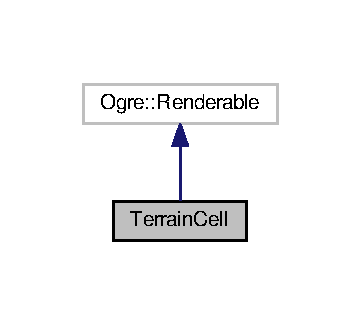
\includegraphics[width=173pt]{class_terrain_cell__inherit__graph}
\end{center}
\end{figure}


Collaboration diagram for Terrain\+Cell\+:\nopagebreak
\begin{figure}[H]
\begin{center}
\leavevmode
\includegraphics[width=173pt]{class_terrain_cell__coll__graph}
\end{center}
\end{figure}
\subsection*{Public Member Functions}
\begin{DoxyCompactItemize}
\item 
\mbox{\Hypertarget{class_terrain_cell_a8e486aba1ecb56796b8398ab712b9ac2}\label{class_terrain_cell_a8e486aba1ecb56796b8398ab712b9ac2}} 
{\bfseries Terrain\+Cell} (\hyperlink{class_graphics_terrain}{Graphics\+Terrain} $\ast$parent\+Terrain)
\item 
\mbox{\Hypertarget{class_terrain_cell_a480311a83246c2048b60a6eba1f3e5c1}\label{class_terrain_cell_a480311a83246c2048b60a6eba1f3e5c1}} 
bool {\bfseries get\+Use\+Skirts} (void) const
\item 
\mbox{\Hypertarget{class_terrain_cell_a4908343e288dd98834c943f73e7dc6ee}\label{class_terrain_cell_a4908343e288dd98834c943f73e7dc6ee}} 
void {\bfseries initialize} (Ogre\+::\+Vao\+Manager $\ast$vao\+Manager, bool use\+Skirts)
\item 
\mbox{\Hypertarget{class_terrain_cell_ab2dd3afcb1879e45b98c54b108cf0204}\label{class_terrain_cell_ab2dd3afcb1879e45b98c54b108cf0204}} 
void {\bfseries set\+Origin} (const \hyperlink{struct_grid_point}{Grid\+Point} \&grid\+Pos, Ogre\+::uint32 horizontal\+Pixel\+Dim, Ogre\+::uint32 vertical\+Pixel\+Dim, Ogre\+::uint32 lod\+Level)
\item 
bool \hyperlink{class_terrain_cell_a18155abf464d4f6d1f3bf59a21eee301}{merge} (\hyperlink{class_terrain_cell}{Terrain\+Cell} $\ast$next)
\item 
\mbox{\Hypertarget{class_terrain_cell_a3d59cf3485f39a7c21411eeaaffcd92a}\label{class_terrain_cell_a3d59cf3485f39a7c21411eeaaffcd92a}} 
void {\bfseries upload\+To\+Gpu} (Ogre\+::uint32 $\ast$R\+E\+S\+T\+R\+I\+C\+T\+\_\+\+A\+L\+I\+AS gpu\+Ptr) const
\item 
\mbox{\Hypertarget{class_terrain_cell_a798bc5d90c5fd2f3a840fb7f6d01d3b4}\label{class_terrain_cell_a798bc5d90c5fd2f3a840fb7f6d01d3b4}} 
virtual const Ogre\+::\+Light\+List \& {\bfseries get\+Lights} (void) const
\item 
\mbox{\Hypertarget{class_terrain_cell_af9cce8bdbcd17ba23a98d49197619f76}\label{class_terrain_cell_af9cce8bdbcd17ba23a98d49197619f76}} 
virtual void {\bfseries get\+Render\+Operation} (Ogre\+::v1\+::\+Render\+Operation \&op, bool caster\+Pass)
\item 
\mbox{\Hypertarget{class_terrain_cell_af87d546b5cdcc1eb14b53f966765b8d4}\label{class_terrain_cell_af87d546b5cdcc1eb14b53f966765b8d4}} 
virtual void {\bfseries get\+World\+Transforms} (Ogre\+::\+Matrix4 $\ast$xform) const
\item 
\mbox{\Hypertarget{class_terrain_cell_ae50fc017b6a731a35c4764df52f46628}\label{class_terrain_cell_ae50fc017b6a731a35c4764df52f46628}} 
virtual bool {\bfseries get\+Casts\+Shadows} (void) const
\end{DoxyCompactItemize}


\subsection{Member Function Documentation}
\mbox{\Hypertarget{class_terrain_cell_a18155abf464d4f6d1f3bf59a21eee301}\label{class_terrain_cell_a18155abf464d4f6d1f3bf59a21eee301}} 
\index{Terrain\+Cell@{Terrain\+Cell}!merge@{merge}}
\index{merge@{merge}!Terrain\+Cell@{Terrain\+Cell}}
\subsubsection{\texorpdfstring{merge()}{merge()}}
{\footnotesize\ttfamily bool Terrain\+Cell\+::merge (\begin{DoxyParamCaption}\item[{\hyperlink{class_terrain_cell}{Terrain\+Cell} $\ast$}]{next }\end{DoxyParamCaption})}

Merges another \hyperlink{class_terrain_cell}{Terrain\+Cell} into \textquotesingle{}this\textquotesingle{} for reducing batch counts. e.\+g. Two 32x32 cells will merge into one 64x32 or 32x64 Two 64x32 cells will merge into one 64x64 A 32x64 cell cannot merge with a 32x32 one. A 64x32 cell cannot merge with a 32x32 one. \begin{DoxyRemark}{Remarks}
Merge will only happen if the cells are of the same L\+OD level and are contiguous. 
\end{DoxyRemark}

\begin{DoxyParams}{Parameters}
{\em next} & The other \hyperlink{class_terrain_cell}{Terrain\+Cell} to merge with. \\
\hline
\end{DoxyParams}
\begin{DoxyReturn}{Returns}
False if couldn\textquotesingle{}t merge, true on success. 
\end{DoxyReturn}


The documentation for this class was generated from the following files\+:\begin{DoxyCompactItemize}
\item 
/home/louis/projects/\+Le\+Dernier\+Morkid/include/\+Terrain/Terrain\+Cell.\+h\item 
/home/louis/projects/\+Le\+Dernier\+Morkid/src/\+Terrain/Terrain\+Cell.\+cpp\end{DoxyCompactItemize}

\hypertarget{struct_terrain_property}{}\section{Terrain\+Property Struct Reference}
\label{struct_terrain_property}\index{Terrain\+Property@{Terrain\+Property}}
\subsection*{Static Public Attributes}
\begin{DoxyCompactItemize}
\item 
\mbox{\Hypertarget{struct_terrain_property_a22095cddb10ad9588af60aac13e91822}\label{struct_terrain_property_a22095cddb10ad9588af60aac13e91822}} 
static const Ogre\+::\+Id\+String {\bfseries Hw\+Gamma\+Read} = Ogre\+::\+Id\+String(\char`\"{}hw\+\_\+gamma\+\_\+read\char`\"{})
\item 
\mbox{\Hypertarget{struct_terrain_property_a522f35e9ece5841d0725970b60d1c109}\label{struct_terrain_property_a522f35e9ece5841d0725970b60d1c109}} 
static const Ogre\+::\+Id\+String {\bfseries Hw\+Gamma\+Write} = Ogre\+::\+Id\+String(\char`\"{}hw\+\_\+gamma\+\_\+write\char`\"{})
\item 
\mbox{\Hypertarget{struct_terrain_property_acf24b762c211bd602ec09a42c99d89c6}\label{struct_terrain_property_acf24b762c211bd602ec09a42c99d89c6}} 
static const Ogre\+::\+Id\+String {\bfseries Signed\+Int\+Tex} = Ogre\+::\+Id\+String(\char`\"{}signed\+\_\+int\+\_\+textures\char`\"{})
\item 
\mbox{\Hypertarget{struct_terrain_property_af3ca6b4b14896385b7f8469d3319b190}\label{struct_terrain_property_af3ca6b4b14896385b7f8469d3319b190}} 
static const Ogre\+::\+Id\+String {\bfseries Materials\+Per\+Buffer} = Ogre\+::\+Id\+String(\char`\"{}materials\+\_\+per\+\_\+buffer\char`\"{})
\item 
\mbox{\Hypertarget{struct_terrain_property_a72ae12a8d7e970352dce12c85ec347e4}\label{struct_terrain_property_a72ae12a8d7e970352dce12c85ec347e4}} 
static const Ogre\+::\+Id\+String {\bfseries Debug\+Pssm\+Splits} = Ogre\+::\+Id\+String(\char`\"{}debug\+\_\+pssm\+\_\+splits\char`\"{})
\item 
\mbox{\Hypertarget{struct_terrain_property_a7e1dd987e92da8748a20dfee723f1323}\label{struct_terrain_property_a7e1dd987e92da8748a20dfee723f1323}} 
static const Ogre\+::\+Id\+String {\bfseries Use\+Skirts} = Ogre\+::\+Id\+String(\char`\"{}use\+\_\+skirts\char`\"{})
\item 
\mbox{\Hypertarget{struct_terrain_property_ade95dfaa0276195af0c8578d32fe674a}\label{struct_terrain_property_ade95dfaa0276195af0c8578d32fe674a}} 
static const Ogre\+::\+Id\+String {\bfseries Num\+Textures} = Ogre\+::\+Id\+String(\char`\"{}num\+\_\+textures\char`\"{})
\item 
\mbox{\Hypertarget{struct_terrain_property_a9b738b34017c423e3f86fb2597c155b4}\label{struct_terrain_property_a9b738b34017c423e3f86fb2597c155b4}} 
static const char $\ast$ {\bfseries Diffuse\+Map} = \char`\"{}diffuse\+\_\+map\char`\"{}
\item 
\mbox{\Hypertarget{struct_terrain_property_aa2b0b5649921f282672b2e5e750ac962}\label{struct_terrain_property_aa2b0b5649921f282672b2e5e750ac962}} 
static const char $\ast$ {\bfseries Env\+Probe\+Map} = \char`\"{}envprobe\+\_\+map\char`\"{}
\item 
\mbox{\Hypertarget{struct_terrain_property_afd2efb252f68c6b60018f39e8c2925f9}\label{struct_terrain_property_afd2efb252f68c6b60018f39e8c2925f9}} 
static const char $\ast$ {\bfseries Detail\+Weight\+Map} = \char`\"{}detail\+\_\+weight\+\_\+map\char`\"{}
\item 
\mbox{\Hypertarget{struct_terrain_property_a4106f05aa014fec64fe6df28ab29437b}\label{struct_terrain_property_a4106f05aa014fec64fe6df28ab29437b}} 
static const char $\ast$ {\bfseries Detail\+MapN} = \char`\"{}detail\+\_\+map\char`\"{}
\item 
\mbox{\Hypertarget{struct_terrain_property_ae519d451e95671036d039c74d04e6be8}\label{struct_terrain_property_ae519d451e95671036d039c74d04e6be8}} 
static const char $\ast$ {\bfseries Detail\+Map\+NmN} = \char`\"{}detail\+\_\+map\+\_\+nm\char`\"{}
\item 
\mbox{\Hypertarget{struct_terrain_property_a3450d96a818009432903ea828a734454}\label{struct_terrain_property_a3450d96a818009432903ea828a734454}} 
static const char $\ast$ {\bfseries Roughness\+Map} = \char`\"{}roughness\+\_\+map\char`\"{}
\item 
\mbox{\Hypertarget{struct_terrain_property_a06fdb464065168c81de14c5a62d9e90d}\label{struct_terrain_property_a06fdb464065168c81de14c5a62d9e90d}} 
static const char $\ast$ {\bfseries Metalness\+Map} = \char`\"{}metalness\+\_\+map\char`\"{}
\item 
\mbox{\Hypertarget{struct_terrain_property_aa4c1809651322a7fbf1c195b1722258e}\label{struct_terrain_property_aa4c1809651322a7fbf1c195b1722258e}} 
static const Ogre\+::\+Id\+String {\bfseries Fresnel\+Scalar} = Ogre\+::\+Id\+String(\char`\"{}fresnel\+\_\+scalar\char`\"{})
\item 
\mbox{\Hypertarget{struct_terrain_property_a99edf6788f3c16492d242822c4af107e}\label{struct_terrain_property_a99edf6788f3c16492d242822c4af107e}} 
static const Ogre\+::\+Id\+String {\bfseries Metallic\+Workflow} = Ogre\+::\+Id\+String(\char`\"{}metallic\+\_\+workflow\char`\"{})
\item 
\mbox{\Hypertarget{struct_terrain_property_a98f5bc977de45a559dbf5d5e3c1e3c38}\label{struct_terrain_property_a98f5bc977de45a559dbf5d5e3c1e3c38}} 
static const Ogre\+::\+Id\+String {\bfseries Receive\+Shadows} = Ogre\+::\+Id\+String(\char`\"{}receive\+\_\+shadows\char`\"{})
\item 
\mbox{\Hypertarget{struct_terrain_property_a15bbb0eaad4efe4b5b339c0b7b7ee2e4}\label{struct_terrain_property_a15bbb0eaad4efe4b5b339c0b7b7ee2e4}} 
static const Ogre\+::\+Id\+String {\bfseries Detail\+Offsets0} = Ogre\+::\+Id\+String(\char`\"{}detail\+\_\+offsets0\char`\"{})
\item 
\mbox{\Hypertarget{struct_terrain_property_a9b3e8a48445dac5ce7cac54905b8a484}\label{struct_terrain_property_a9b3e8a48445dac5ce7cac54905b8a484}} 
static const Ogre\+::\+Id\+String {\bfseries Detail\+Offsets1} = Ogre\+::\+Id\+String(\char`\"{}detail\+\_\+offsets1\char`\"{})
\item 
\mbox{\Hypertarget{struct_terrain_property_a3c5a1b12221828b81aa299fea835fc82}\label{struct_terrain_property_a3c5a1b12221828b81aa299fea835fc82}} 
static const Ogre\+::\+Id\+String {\bfseries Detail\+Offsets2} = Ogre\+::\+Id\+String(\char`\"{}detail\+\_\+offsets2\char`\"{})
\item 
\mbox{\Hypertarget{struct_terrain_property_af1e758c0b5680f59fe17fbc73b116510}\label{struct_terrain_property_af1e758c0b5680f59fe17fbc73b116510}} 
static const Ogre\+::\+Id\+String {\bfseries Detail\+Offsets3} = Ogre\+::\+Id\+String(\char`\"{}detail\+\_\+offsets3\char`\"{})
\item 
\mbox{\Hypertarget{struct_terrain_property_abbf7f88e8da966c767bcf4aea5c61172}\label{struct_terrain_property_abbf7f88e8da966c767bcf4aea5c61172}} 
static const Ogre\+::\+Id\+String {\bfseries Detail\+Maps\+Diffuse} = Ogre\+::\+Id\+String(\char`\"{}detail\+\_\+maps\+\_\+diffuse\char`\"{})
\item 
\mbox{\Hypertarget{struct_terrain_property_ae09627b2abaced813e27ecdf710a0ea0}\label{struct_terrain_property_ae09627b2abaced813e27ecdf710a0ea0}} 
static const Ogre\+::\+Id\+String {\bfseries Detail\+Maps\+Normal} = Ogre\+::\+Id\+String(\char`\"{}detail\+\_\+maps\+\_\+normal\char`\"{})
\item 
\mbox{\Hypertarget{struct_terrain_property_aab108a9b0dbd22b8aa2a93c7d6c45b82}\label{struct_terrain_property_aab108a9b0dbd22b8aa2a93c7d6c45b82}} 
static const Ogre\+::\+Id\+String {\bfseries First\+Valid\+Detail\+Map\+Nm} = Ogre\+::\+Id\+String(\char`\"{}first\+\_\+valid\+\_\+detail\+\_\+map\+\_\+nm\char`\"{})
\item 
\mbox{\Hypertarget{struct_terrain_property_a89f0b09e8c25338b07c18b6cbdde79d3}\label{struct_terrain_property_a89f0b09e8c25338b07c18b6cbdde79d3}} 
static const Ogre\+::\+Id\+String {\bfseries Pcf3x3} = Ogre\+::\+Id\+String(\char`\"{}pcf\+\_\+3x3\char`\"{})
\item 
\mbox{\Hypertarget{struct_terrain_property_a9cb2afcb4970a29cdce9467cf8924079}\label{struct_terrain_property_a9cb2afcb4970a29cdce9467cf8924079}} 
static const Ogre\+::\+Id\+String {\bfseries Pcf4x4} = Ogre\+::\+Id\+String(\char`\"{}pcf\+\_\+4x4\char`\"{})
\item 
\mbox{\Hypertarget{struct_terrain_property_a0b0db17f3711b9133dd51d1d004fc3fa}\label{struct_terrain_property_a0b0db17f3711b9133dd51d1d004fc3fa}} 
static const Ogre\+::\+Id\+String {\bfseries Pcf\+Iterations} = Ogre\+::\+Id\+String(\char`\"{}pcf\+\_\+iterations\char`\"{})
\item 
\mbox{\Hypertarget{struct_terrain_property_ac6065b41bb892cb13bcdc97a7e421856}\label{struct_terrain_property_ac6065b41bb892cb13bcdc97a7e421856}} 
static const Ogre\+::\+Id\+String {\bfseries Env\+Map\+Scale} = Ogre\+::\+Id\+String(\char`\"{}envmap\+\_\+scale\char`\"{})
\item 
\mbox{\Hypertarget{struct_terrain_property_af28e06830806f5eacffd56d180aae06f}\label{struct_terrain_property_af28e06830806f5eacffd56d180aae06f}} 
static const Ogre\+::\+Id\+String {\bfseries Ambient\+Fixed} = Ogre\+::\+Id\+String(\char`\"{}ambient\+\_\+fixed\char`\"{})
\item 
\mbox{\Hypertarget{struct_terrain_property_a4958d05abfac1cb149b7908f203bc807}\label{struct_terrain_property_a4958d05abfac1cb149b7908f203bc807}} 
static const Ogre\+::\+Id\+String {\bfseries Ambient\+Hemisphere} = Ogre\+::\+Id\+String(\char`\"{}ambient\+\_\+hemisphere\char`\"{})
\item 
\mbox{\Hypertarget{struct_terrain_property_a300b3f59540f0f9e19fc5b54b89513dc}\label{struct_terrain_property_a300b3f59540f0f9e19fc5b54b89513dc}} 
static const Ogre\+::\+Id\+String {\bfseries Brdf\+Default} = Ogre\+::\+Id\+String(\char`\"{}B\+R\+D\+F\+\_\+\+Default\char`\"{})
\item 
\mbox{\Hypertarget{struct_terrain_property_aa8fc06beb53007f23df7c61d973fdfc1}\label{struct_terrain_property_aa8fc06beb53007f23df7c61d973fdfc1}} 
static const Ogre\+::\+Id\+String {\bfseries Brdf\+Cook\+Torrance} = Ogre\+::\+Id\+String(\char`\"{}B\+R\+D\+F\+\_\+\+Cook\+Torrance\char`\"{})
\item 
\mbox{\Hypertarget{struct_terrain_property_a47eef3266703c4b57e7a41d5c31af4bb}\label{struct_terrain_property_a47eef3266703c4b57e7a41d5c31af4bb}} 
static const Ogre\+::\+Id\+String {\bfseries Fresnel\+Separate\+Diffuse} = Ogre\+::\+Id\+String(\char`\"{}fresnel\+\_\+separate\+\_\+diffuse\char`\"{})
\item 
\mbox{\Hypertarget{struct_terrain_property_ac5d4c929036f2bdb2959da73f70a2ab6}\label{struct_terrain_property_ac5d4c929036f2bdb2959da73f70a2ab6}} 
static const Ogre\+::\+Id\+String {\bfseries Ggx\+Height\+Correlated} = Ogre\+::\+Id\+String(\char`\"{}G\+G\+X\+\_\+height\+\_\+correlated\char`\"{})
\item 
static const Ogre\+::\+Id\+String $\ast$ {\bfseries Detail\+Offsets\+Ptrs} \mbox{[}4\mbox{]}
\end{DoxyCompactItemize}


\subsection{Detailed Description}


Definition at line 188 of file Hlms\+Terrain.\+h.



\subsection{Member Data Documentation}
\mbox{\Hypertarget{struct_terrain_property_ac7f6e9bf302538090e3c9155799304b8}\label{struct_terrain_property_ac7f6e9bf302538090e3c9155799304b8}} 
\index{Terrain\+Property@{Terrain\+Property}!Detail\+Offsets\+Ptrs@{Detail\+Offsets\+Ptrs}}
\index{Detail\+Offsets\+Ptrs@{Detail\+Offsets\+Ptrs}!Terrain\+Property@{Terrain\+Property}}
\subsubsection{\texorpdfstring{Detail\+Offsets\+Ptrs}{DetailOffsetsPtrs}}
{\footnotesize\ttfamily const Ogre\+::\+Id\+String $\ast$ Terrain\+Property\+::\+Detail\+Offsets\+Ptrs\hspace{0.3cm}{\ttfamily [static]}}

{\bfseries Initial value\+:}
\begin{DoxyCode}
=
        \{
                &TerrainProperty::DetailOffsets0,
                &TerrainProperty::DetailOffsets1,
                &TerrainProperty::DetailOffsets2,
                &TerrainProperty::DetailOffsets3\}
\end{DoxyCode}


Definition at line 232 of file Hlms\+Terrain.\+h.



The documentation for this struct was generated from the following files\+:\begin{DoxyCompactItemize}
\item 
/home/louis/projects/\+Le\+Dernier\+Morkid/include/\+Terrain/\+Hlms/Hlms\+Terrain.\+h\item 
/home/louis/projects/\+Le\+Dernier\+Morkid/src/\+Terrain/\+Hlms/Hlms\+Terrain.\+cpp\end{DoxyCompactItemize}

\hypertarget{struct_thread_data}{}\section{Thread\+Data Struct Reference}
\label{struct_thread_data}\index{Thread\+Data@{Thread\+Data}}


Inheritance diagram for Thread\+Data\+:\nopagebreak
\begin{figure}[H]
\begin{center}
\leavevmode
\includegraphics[width=216pt]{struct_thread_data__inherit__graph}
\end{center}
\end{figure}
\subsection*{Public Attributes}
\begin{DoxyCompactItemize}
\item 
\mbox{\Hypertarget{struct_thread_data_a09870ee767fb0882817702c7fccce29d}\label{struct_thread_data_a09870ee767fb0882817702c7fccce29d}} 
Ogre\+::\+Barrier $\ast$ {\bfseries barrier}
\end{DoxyCompactItemize}


The documentation for this struct was generated from the following file\+:\begin{DoxyCompactItemize}
\item 
/home/louis/projects/\+Le\+Dernier\+Morkid/\+Common/include/\+Threading/Thread\+Manager.\+h\end{DoxyCompactItemize}

\hypertarget{class_thread_manager}{}\section{Thread\+Manager Class Reference}
\label{class_thread_manager}\index{Thread\+Manager@{Thread\+Manager}}


Inheritance diagram for Thread\+Manager\+:\nopagebreak
\begin{figure}[H]
\begin{center}
\leavevmode
\includegraphics[width=168pt]{class_thread_manager__inherit__graph}
\end{center}
\end{figure}


Collaboration diagram for Thread\+Manager\+:\nopagebreak
\begin{figure}[H]
\begin{center}
\leavevmode
\includegraphics[width=185pt]{class_thread_manager__coll__graph}
\end{center}
\end{figure}
\subsection*{Public Member Functions}
\begin{DoxyCompactItemize}
\item 
\mbox{\Hypertarget{class_thread_manager_a7f63f89915ef17f37f741ae29c19682f}\label{class_thread_manager_a7f63f89915ef17f37f741ae29c19682f}} 
virtual void {\bfseries register\+Thread} (Thread\+Func thread, Ogre\+::\+T\+H\+R\+E\+A\+D\+\_\+\+E\+N\+T\+R\+Y\+\_\+\+P\+O\+I\+NT internal\+Thread)
\item 
\mbox{\Hypertarget{class_thread_manager_afec21d2b814f77ef06221f0529e6e8b4}\label{class_thread_manager_afec21d2b814f77ef06221f0529e6e8b4}} 
virtual void {\bfseries run} ()
\item 
\mbox{\Hypertarget{class_thread_manager_a3dbe938c3fa9b2202d84c5b623db74a4}\label{class_thread_manager_a3dbe938c3fa9b2202d84c5b623db74a4}} 
virtual void {\bfseries set\+Thread\+Data} (\hyperlink{struct_thread_data}{Thread\+Data} $\ast$thread\+Data)
\item 
\mbox{\Hypertarget{class_thread_manager_a00c6fbd9feafca3e5408bc7a0fa7d0e5}\label{class_thread_manager_a00c6fbd9feafca3e5408bc7a0fa7d0e5}} 
virtual \hyperlink{struct_thread_data}{Thread\+Data} $\ast$ {\bfseries get\+Thread\+Data} ()
\end{DoxyCompactItemize}
\subsection*{Protected Attributes}
\begin{DoxyCompactItemize}
\item 
\mbox{\Hypertarget{class_thread_manager_a6b3e5e01419d3419ac09cefc6748f9e0}\label{class_thread_manager_a6b3e5e01419d3419ac09cefc6748f9e0}} 
std\+::vector$<$ std\+::pair$<$ Thread\+Func, Ogre\+::\+T\+H\+R\+E\+A\+D\+\_\+\+E\+N\+T\+R\+Y\+\_\+\+P\+O\+I\+NT $>$ $>$ {\bfseries m\+Registered\+Threads}
\item 
\mbox{\Hypertarget{class_thread_manager_a8bce7db0b6a5369556a31d906cb30ff1}\label{class_thread_manager_a8bce7db0b6a5369556a31d906cb30ff1}} 
\hyperlink{struct_thread_data}{Thread\+Data} $\ast$ {\bfseries m\+Thread\+Data}
\end{DoxyCompactItemize}


The documentation for this class was generated from the following files\+:\begin{DoxyCompactItemize}
\item 
/home/louis/projects/\+Le\+Dernier\+Morkid/\+Common/include/\+Threading/Thread\+Manager.\+h\item 
/home/louis/projects/\+Le\+Dernier\+Morkid/\+Common/src/\+Threading/Thread\+Manager.\+cpp\end{DoxyCompactItemize}

\hypertarget{class_common_1_1_yield_timer}{}\section{Common\+:\+:Yield\+Timer Class Reference}
\label{class_common_1_1_yield_timer}\index{Common\+::\+Yield\+Timer@{Common\+::\+Yield\+Timer}}
\subsection*{Public Member Functions}
\begin{DoxyCompactItemize}
\item 
\mbox{\Hypertarget{class_common_1_1_yield_timer_a4d1c12e6e3f5e825d796286f0c1e2345}\label{class_common_1_1_yield_timer_a4d1c12e6e3f5e825d796286f0c1e2345}} 
{\bfseries Yield\+Timer} (Ogre\+::\+Timer $\ast$external\+Timer)
\item 
\mbox{\Hypertarget{class_common_1_1_yield_timer_a55ba2e4b796cc59768c5200cc38d303c}\label{class_common_1_1_yield_timer_a55ba2e4b796cc59768c5200cc38d303c}} 
unsigned long {\bfseries yield} (double frame\+Time, unsigned long start\+Time)
\end{DoxyCompactItemize}


The documentation for this class was generated from the following file\+:\begin{DoxyCompactItemize}
\item 
/home/louis/projects/\+Le\+Dernier\+Morkid/\+Common/include/\+Threading/Yield\+Timer.\+h\end{DoxyCompactItemize}

%--- End generated contents ---

% Index
\backmatter
\newpage
\phantomsection
\clearemptydoublepage
\addcontentsline{toc}{chapter}{Index}
\printindex

\end{document}
